\documentclass{tufte-book}\usepackage[]{graphicx}\usepackage[]{color}
%% maxwidth is the original width if it is less than linewidth
%% otherwise use linewidth (to make sure the graphics do not exceed the margin)
\makeatletter
\def\maxwidth{ %
  \ifdim\Gin@nat@width>\linewidth
    \linewidth
  \else
    \Gin@nat@width
  \fi
}
\makeatother

\usepackage{Sweavel}


\usepackage[flexible]{optional}
\usepackage{tufte-larger}
\usepackage[some]{background}
\usepackage{amssymb,amsmath}
\usepackage{amsmath, amssymb,txfonts,bm}
\usepackage{checkend}
\usepackage{nextpage}
\usepackage{listings}
\usepackage{framed}
\usepackage{float}
\usepackage{colortbl}
\usepackage{cprotect}
\usepackage{enumitem}
\usepackage{makeidx}
\makeindex
\usepackage{index}
\usepackage{multicol}
\newindex{fun}{fdx}{fnd}{Index of R Symbols and Functions}

% \newenvironment{knitrout}{\setlength{\topsep}{0mm}}{}
% \newcommand{\flexicol}{fullflexible}
\newcommand{\flexicol}{fixed}

\lstdefinestyle{Rstyle}{%
  fancyvrb=false,escapechar=`,language=R,%
  basicstyle={\Rcolor\Sweavesize\ttfamily},%         Added \ttfamily
  backgroundcolor=\Rbackground,%
  showstringspaces=false,%
  keywordstyle=\Rcolor,%
  commentstyle={\Rcommentcolor\ttfamily\itshape},%
  %literate=                                         Removed
  alsoother={$},%
  alsoletter={.<-},%
  otherkeywords={!,!=,~,$,*,\&,\%/\%,\%*\%,\%\%,<-,<<-,/},%
  escapeinside={(*}{*)}}%

\makeatletter
\renewenvironment{theindex}{%
  \columnseprule \z@
  \columnsep 35\p@
\begin{multicols}{3}[\chapter*{\indexname}][10\baselineskip]%
  \addcontentsline{toc}{chapter}{\indexname}%
  \setlength\parindent{0pt}\pagestyle{plain}\let\item\@idxitem}
{\end{multicols}}
\makeatother

\hypersetup{colorlinks}% uncomment this line if you prefer colored hyperlinks (e.g., for onscreen viewing)

%%
% Book metadata
\title{Learning and Exploring R}
\author[]{J H Maindonald}
\publisher{}

%%
% If they're installed, use Bergamo and Chantilly from www.fontsite.com.
% They're clones of Bembo and Gill Sans, respectively.
%\IfFileExists{bergamo.sty}{\usepackage[osf]{bergamo}}{}% Bembo
%\IfFileExists{chantill.sty}{\usepackage{chantill}}{}% Gill Sans

%\usepackage{microtype}

%%
% For nicely typeset tabular material
\usepackage{booktabs}

%%
% For graphics / images
\usepackage{graphicx}
\setkeys{Gin}{width=\linewidth,totalheight=\textheight,keepaspectratio}
\graphicspath{{figs/}}

% The fancyvrb package lets us customize the formatting of verbatim
% environments.  We use a slightly smaller font.
\usepackage{relsize,fancyvrb}
\fvset{fontsize=\normalsize}

%%
% Prints argument within hanging parentheses (i.e., parentheses that take
% up no horizontal space).  Useful in tabular environments.
\newcommand{\hangp}[1]{\makebox[0pt][r]{(}#1\makebox[0pt][l]{)}}

%%
% Prints an asterisk that takes up no horizontal space.
% Useful in tabular environments.
\newcommand{\hangstar}{\makebox[0pt][l]{*}}

%%
% Prints a trailing space in a smart way.
\usepackage{xspace}

%%
% Some shortcuts for Tufte's book titles.  The lowercase commands will
% produce the initials of the book title in italics.  The all-caps commands
% will print out the full title of the book in italics.
\newcommand{\vdqi}{\textit{VDQI}\xspace}
\newcommand{\ei}{\textit{EI}\xspace}
\newcommand{\ve}{\textit{VE}\xspace}
\newcommand{\be}{\textit{BE}\xspace}
\newcommand{\VDQI}{\textit{The Visual Display of Quantitative Information}\xspace}
\newcommand{\EI}{\textit{Envisioning Information}\xspace}
\newcommand{\VE}{\textit{Visual Explanations}\xspace}
\newcommand{\BE}{\textit{Beautiful Evidence}\xspace}

\newcommand{\TL}{Tufte-\LaTeX\xspace}

% Prints the month name (e.g., January) and the year (e.g., 2008)
\newcommand{\monthyear}{%
  \ifcase\month\or January\or February\or March\or April\or May\or June\or
  July\or August\or September\or October\or November\or
  December\fi\space\number\year
}

\renewcommand{\maketitlepage}[0]{%
  \cleardoublepage%
  {%
  \sffamily%
  \begin{fullwidth}%
  \fontsize{18}{20}\selectfont\par\noindent\textcolor{darkgray}{{\thanklessauthor}}%
  \vspace{11.5pc}%
%  \fontsize{27}{30}\selectfont\par\noindent\textcolor{darkgray}{{\thanklesstitle}}%
  \fontsize{40}{45}\selectfont\par\noindent\textcolor{darkgray}{{\thanklesstitle}}%
  \vfill%
  \fontsize{14}{16}\selectfont\par\noindent\allcaps{\thanklesspublisher}%
  \end{fullwidth}%
  }
  \thispagestyle{empty}%
  \clearpage%
}


% Prints an epigraph and speaker in sans serif, all-caps type.
\newcommand{\openepigraph}[2]{%
  %\sffamily\fontsize{14}{16}\selectfont
  \begin{fullwidth}
  \sffamily\large
  \begin{doublespace}
  \noindent{#1}\\% epigraph
  \noindent{#2}% author
  \end{doublespace}
  \end{fullwidth}
}

% Inserts a blank page
\newcommand{\blankpage}{\newpage\hbox{}\thispagestyle{empty}\newpage}

\usepackage{units}

% Typesets the font size, leading, and measure in the form of 10/12x26 pc.
\newcommand{\measure}[3]{#1/#2$\times$\unit[#3]{pc}}

% Macros for typesetting the documentation
\newcommand{\hlred}[1]{\textcolor{Maroon}{#1}}% prints in red
\newcommand{\hangleft}[1]{\makebox[0pt][r]{#1}}
\newcommand{\hairsp}{\hspace{1pt}}% hair space
\newcommand{\hquad}{\hskip0.5em\relax}% half quad space
\newcommand{\TODO}{\textcolor{red}{\bf TODO!}\xspace}
\newcommand{\ie}{\textit{i.\hairsp{}e.}\xspace}
\newcommand{\eg}{\textit{e.\hairsp{}g.}\xspace}
\newcommand{\na}{\quad--}% used in tables for N/A cells
\providecommand{\XeLaTeX}{X\lower.5ex\hbox{\kern-0.15em\reflectbox{E}}\kern-0.1em\LaTeX}
\newcommand{\tXeLaTeX}{\XeLaTeX\index{XeLaTeX@\protect\XeLaTeX}}
% \index{\texttt{\textbackslash xyz}@\hangleft{\texttt{\textbackslash}}\texttt{xyz}}
\newcommand{\tuftebs}{\symbol{'134}}% a backslash in tt type in OT1/T1
\newcommand{\doccmdnoindex}[2][]{\texttt{\tuftebs#2}}% command name -- adds backslash automatically (and doesn't add cmd to the index)
\newcommand{\doccmddef}[2][]{%
  \hlred{\texttt{\tuftebs#2}}\label{cmd:#2}%
  \ifthenelse{\isempty{#1}}%
    {% add the command to the index
      \index{#2 command@\protect\hangleft{\texttt{\tuftebs}}\texttt{#2}}% command name
    }%
    {% add the command and package to the index
      \index{#2 command@\protect\hangleft{\texttt{\tuftebs}}\texttt{#2} (\texttt{#1} package)}% command name
      \index{#1 package@\texttt{#1} package}\index{packages!#1@\texttt{#1}}% package name
    }%
}% command name -- adds backslash automatically
\newcommand{\doccmd}[2][]{%
  \texttt{\tuftebs#2}%
  \ifthenelse{\isempty{#1}}%
    {% add the command to the index
      \index{#2 command@\protect\hangleft{\texttt{\tuftebs}}\texttt{#2}}% command name
    }%
    {% add the command and package to the index
      \index{#2 command@\protect\hangleft{\texttt{\tuftebs}}\texttt{#2} (\texttt{#1} package)}% command name
      \index{#1 package@\texttt{#1} package}\index{packages!#1@\texttt{#1}}% package name
    }%
}% command name -- adds backslash automatically
\newcommand{\docopt}[1]{\ensuremath{\langle}\textrm{\textit{#1}}\ensuremath{\rangle}}% optional command argument
\newcommand{\docarg}[1]{\textrm{\textit{#1}}}% (required) command argument
\newenvironment{docspec}{\begin{quotation}\ttfamily\parskip0pt\parindent0pt\ignorespaces}{\end{quotation}}% command specification environment
\newcommand{\docenv}[1]{\texttt{#1}\index{#1 environment@\texttt{#1} environment}\index{environments!#1@\texttt{#1}}}% environment name
\newcommand{\docenvdef}[1]{\hlred{\texttt{#1}}\label{env:#1}\index{#1 environment@\texttt{#1} environment}\index{environments!#1@\texttt{#1}}}% environment name
\newcommand{\docpkg}[1]{\texttt{#1}\index{#1 package@\texttt{#1} package}\index{packages!#1@\texttt{#1}}}% package name
\newcommand{\doccls}[1]{\texttt{#1}}% document class name
\newcommand{\docclsopt}[1]{\texttt{#1}\index{#1 class option@\texttt{#1} class option}\index{class options!#1@\texttt{#1}}}% document class option name
\newcommand{\docclsoptdef}[1]{\hlred{\texttt{#1}}\label{clsopt:#1}\index{#1 class option@\texttt{#1} class option}\index{class options!#1@\texttt{#1}}}% document class option name defined
\newcommand{\docmsg}[2]{\bigskip\begin{fullwidth}\noindent\ttfamily#1\end{fullwidth}\medskip\par\noindent#2}
\newcommand{\docfilehook}[2]{\texttt{#1}\index{file hooks!#2}\index{#1@\texttt{#1}}}
\newcommand{\doccounter}[1]{\texttt{#1}\index{#1 counter@\texttt{#1} counter}}

% Generates the index
% \usepackage{makeidx}

% \definecolor{fgcolor}{rgb}{0.345, 0.345, 0.345}
\definecolor{light}{gray}{.9}
\definecolor{gray40}{gray}{.4}
\definecolor{gray80}{gray}{.8}
\definecolor{gray90}{gray}{.9}

\newcommand{\txtt}[1]{\texttt{#1}}
\newcommand{\margtt}[1]{{\footnotesize \texttt{#1}}}

 \lstnewenvironment{verbcode}
 {\lstset{language=R, xleftmargin=4pt, frame=single, framerule=0pt,
          basicstyle=\small\ttfamily,
         columns=\flexicol,
          showstringspaces=false, backgroundcolor=\color{light}}}
 {}

\newenvironment{itemizz}%
  {\begin{itemize} %
    \setlength{\itemsep}{2pt}%
    \setlength{\parskip}{2pt}} %
  {\end{itemize}}

\begin{document}
% Front matter
\frontmatter




%

\setsidenotefont{\small}
\setcaptionfont{\small}
\setmarginnotefont{\small}
% \setcitationfont

\SetBgContents{
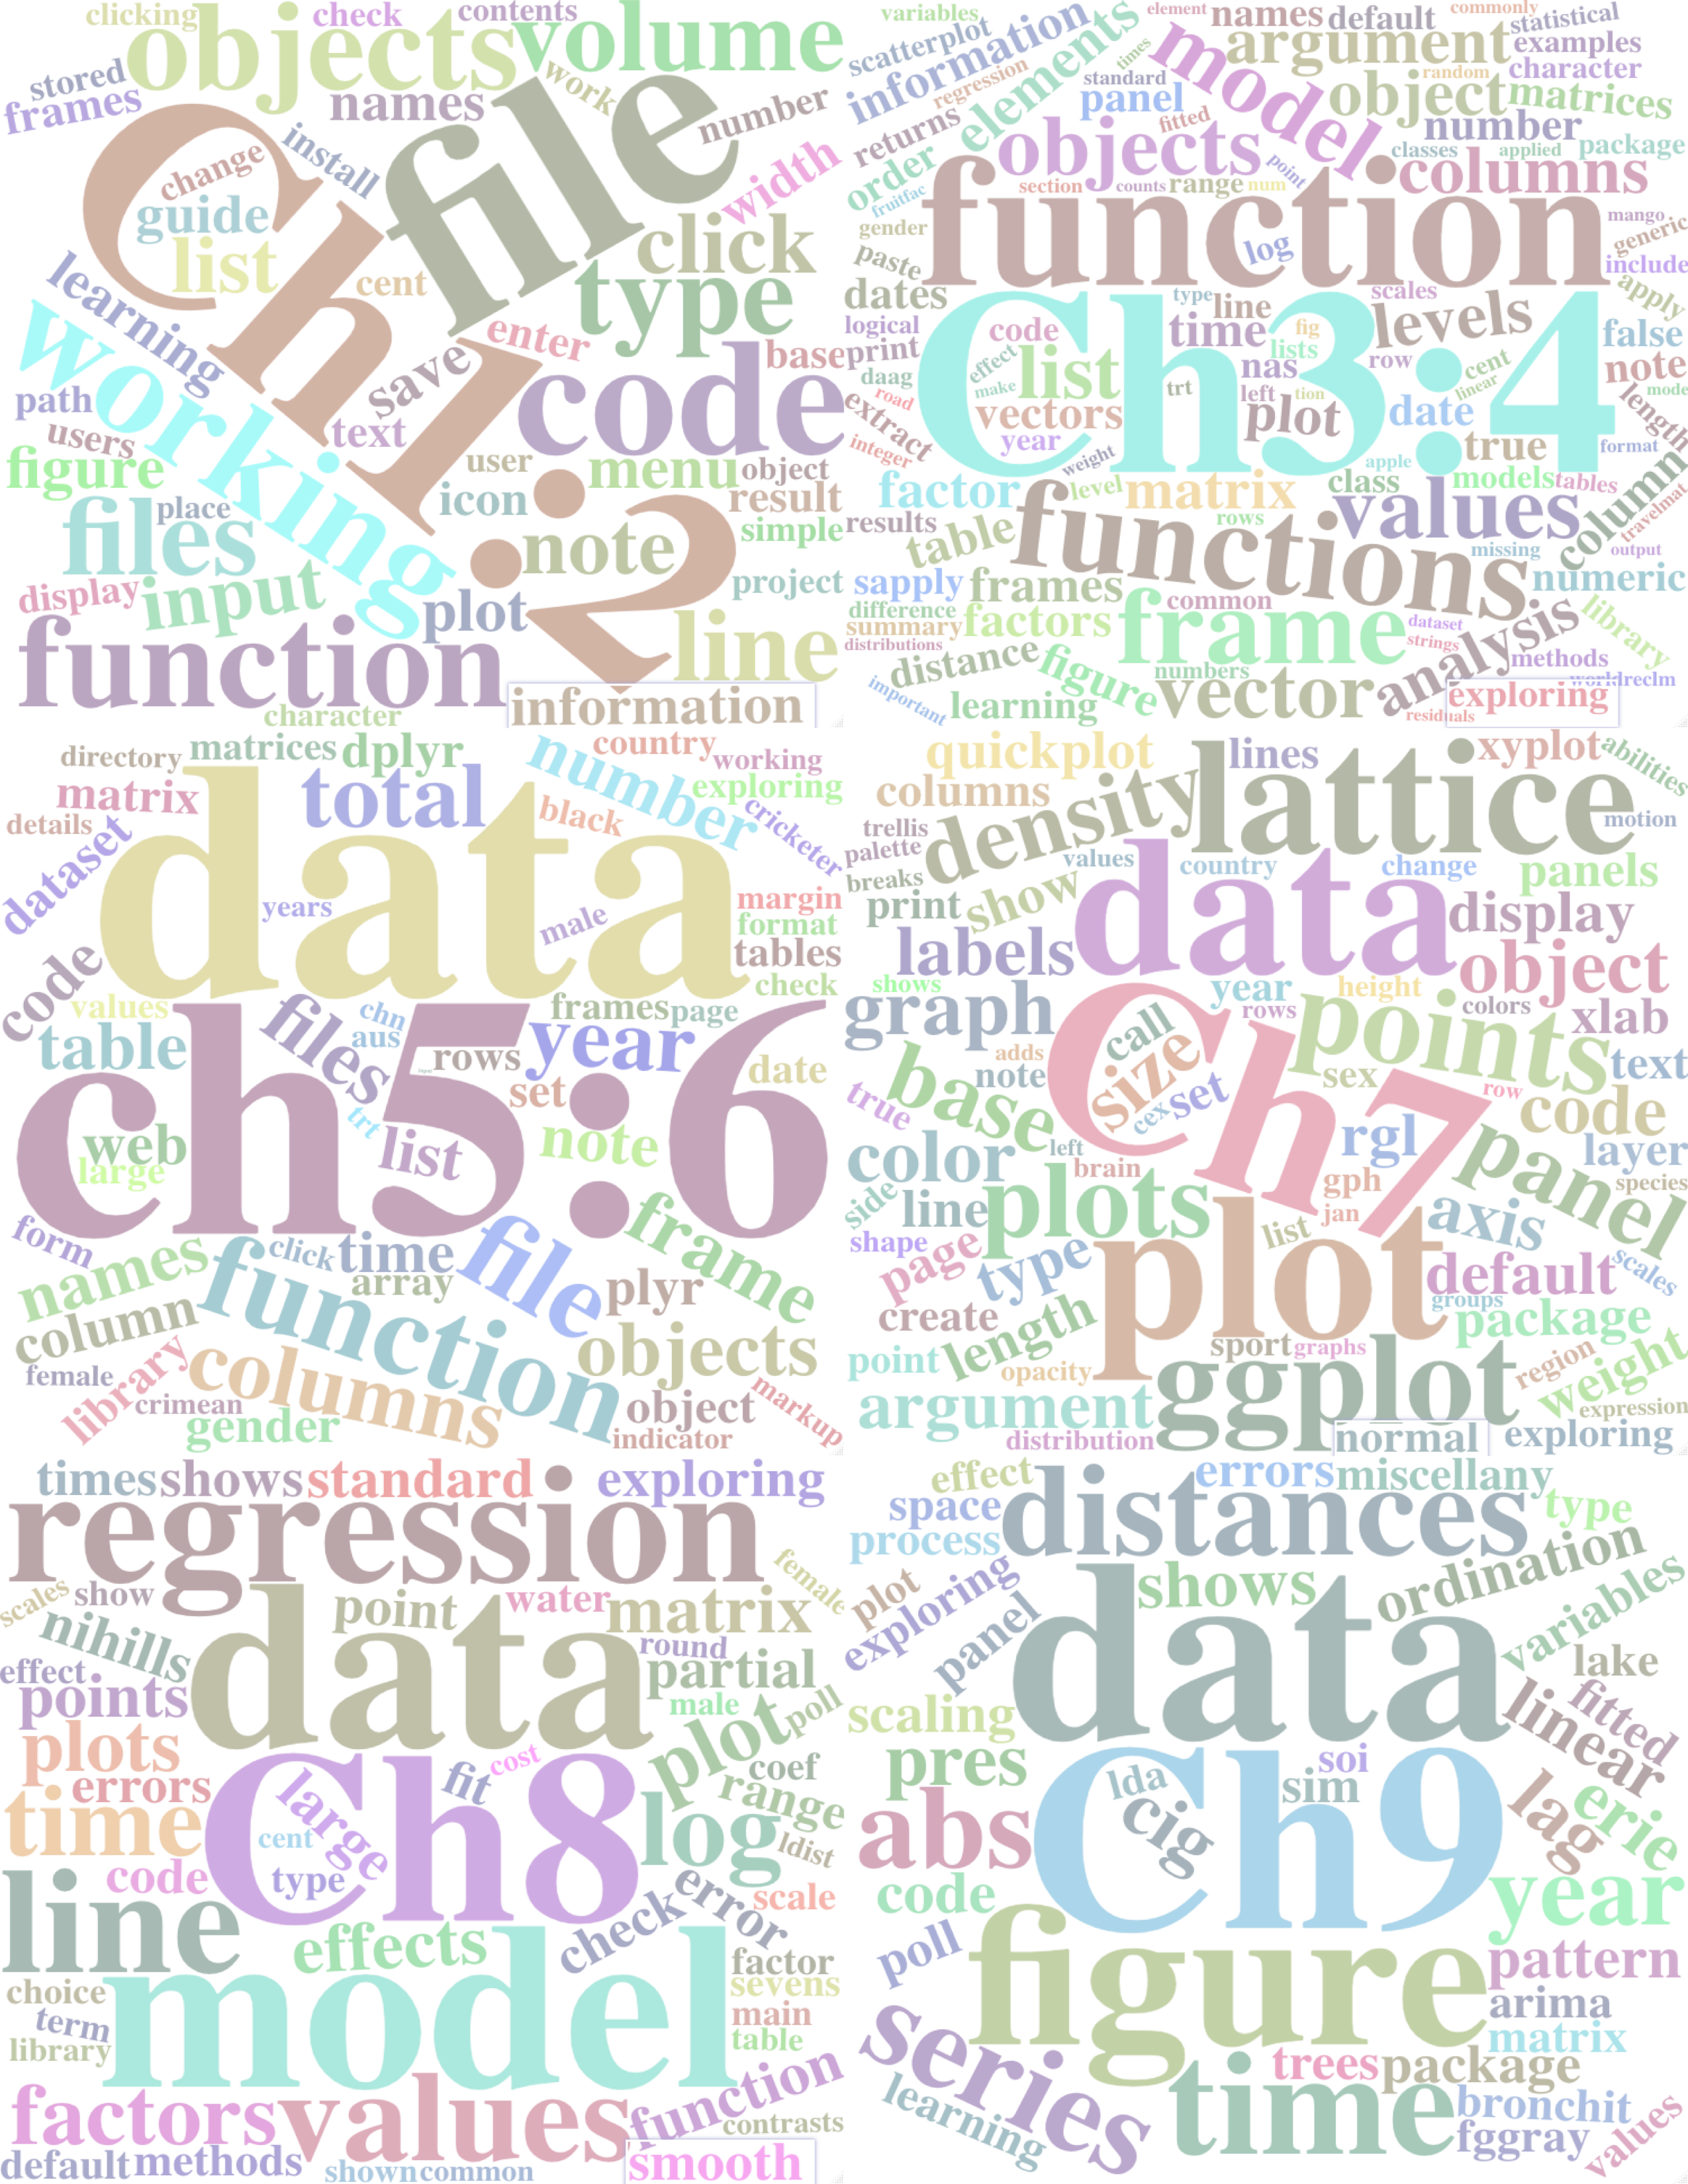
\includegraphics{figs-inc/cover-bg.pdf}
}
\SetBgScale{3.5}
\SetBgColor{gray!70}
\SetBgOpacity{0.2}
\BgThispage
\bmdefine\bX{\mathbf{X}}
\bmdefine\bP{\mathbf{P}}
\bmdefine\sfX{\bm{\textsf{\textmd{X}}}}
% \pagestyle{headings}

% r.1 blank page
% \blankpage

% v.2 epigraphs
% r.3 full title page
\maketitle

% v.4 copyright page
\newpage
\begin{fullwidth}
~\vfill
\thispagestyle{empty}
\setlength{\parindent}{0pt}
\setlength{\parskip}{\baselineskip}
Copyright \copyright\ \the\year\ \thanklessauthor\\
This text is dual licensed under the Creative Commons Attribution-ShareAlike 3.0 Unported License (CC-BY-SA) and the GNU Free Documentation License (GFDL). 

% \par\smallcaps{Published by \thanklesspublisher}

% \par\smallcaps{tufte-latex.googlecode.com}

\par\textit{\monthyear}
\end{fullwidth}
\vfill

\thispagestyle{empty}
\openepigraph{%
S has forever altered the way people analyze, visualize, and
manipulate data... S is an elegant, widely accepted, and enduring
software system, with conceptual integrity, thanks to the insight,
taste, and effort of John Chambers.
}{{\itshape From the citation for the 1998 Association for Computing Machinery
Software award.}
}
\vfill
\openepigraph{%
A big computer, a complex algorithm and a long time does not equal
science.
}{Robert Gentleman}
\vfill


%
% r.5 contents
\tableofcontents


% \begin{fullwidth}
% \listoffigures
% \end{fullwidth}

% \listoftables

% r.7 dedication
% \cleardoublepage
% ~\vfill
% \begin{doublespace}
% \noindent\fontsize{18}{22}\selectfont\itshape
% \nohyphenation
% Dedicated to the creators of S and R.
% \end{doublespace}
% \vfill
% \vfill

% r.9 introduction
\cleardoublepage
\chapter*{Introduction}

% !Rnw root = learnR.Rnw




\section*{The scope of these notes}

These notes were developed over the course of more than a
decade, for use in R courses that were presented to groups
within universities, within CSIRO, and within Government
departments.  Each new course offered the chance to 
extend and refine the content, and to add content that
was tuned to the requirements of the new audience.  
The result is a somewhat eclectic mix of material.
The notes are provided here with the intention that
others will be free to add to them, or to develop them
for their own purposes.
%
%
\section*{Commentary on R}

\subsection*{General}
R has extensive \marginnote{R is free to download from a CRAN site
  (see above).  It runs on all common types of system -- Windows, Mac,
  Unix and Linux.}  graphical abilities that are tightly linked with
its analytic abilities. A new release of base R, on which everything
else is built appears every few months.

The major part of R's abilities for statistical analysis
and for specialist graphics comes from the extensive enhancements that
the packages build on top of the base system.  Its abilities are
further extended by an extensive range of interfaces into
other systems\sidenote{These include Python, SQL and other
  databases, parallel computing using MPI, and Excel.}

The main part of the R system -- base R plus the recommended packages
-- is under continuing development.

\subsection*{The R user base}

Statistical and allied professionals\marginnote{ The R Task Views web
  page (\url{http://cran.csiro.au/web/views/}) notes, for application
  areas where R is widely used, relevant packages.} have found R
  especially attractive, both for the access that it gives to
  cutting edge tools, and as a platform for developing new tools.
Additionally, the R system has found wide use among working
scientists whose data analysis requirements justify the time
needed to gain the necessary R skills.  It is finding use, also, as
an environment in which to embed applications whose primary focus
is not data analysis or graphics.


\subsection*{Getting help}

\begin{fullwidth}
\fbox{\parbox{1.15\textwidth}{
{\bf Note the web sites:}\\[4pt]
Wikipedia:\newline
\url{http://en.wikipedia.org/wiki/R_(programming_language)}\\[3pt]
R-downunder (low traffic, friendly):\newline
\url{http://www.stat.auckland.ac.nz/mailman/listinfo/r-downunder}\\[3pt]
Stackoverflow\newline
\url{http://stackoverflow.com/questions/tagged/r}.
}}
\end{fullwidth}
\vspace*{8pt}

The r-help mailing list\marginnote{Details of this and other lists can
  be found at: \url{http://www.r-project.org}. Be sure to check the
  available documentation before posting to r-help. List archives can
  be searched for previous questions and answers.}  serves, especially
for users with a technical bent, as an informal support network.  The
R community expects users to want more than a quick cook-book fix, and
to show a willingness to work at improving statistical knowledge.

Novices will find the low traffic R-downunder list more friendly and
helpful than the main R mailing list. Its subscribers include some
highly expert individuals.

\subsection*{Important R web links}

\marginnote{CRAN is the primary R `repository'.  Among
  package repositories that supplement CRAN, note in
  particular the Bioconductor repository
  (\url{http://www.bioconductor.org}), which caters for
  high throughput genomic data.}
\noindent
\fbox{\parbox{\textwidth}{
{\bf Note the following web sites:}\\[4pt]
CRAN (Comprehensive R Archive Network):\newline
\url{http://cran.r-project.org}\\[3pt]
Obtain R and R packages from a CRAN mirror in the local region.
An Australian mirror (one of two) is: \url{https://cran.csiro.au/}\\[3pt]
For New Zealand, use \url{http://cran.stat.auckland.ac.nz}\\
R homepage: \url{https://www.r-project.org/}\\[3pt]

For various useful links click, from an R session that uses the
GUI, on the menu item \underline{R help}. Then, on the browser window
that pops up, look under \underline{Resources}}}



\subsection*{The origins and future of R}

The R system implements a dialect of the S language \marginnote{Open
  source systems that might have been the basis for an R-like project
  include Scilab, Octave, Gauss, Lisp-Stat, Python, and now Julia.
  None of these match the range and depth of R's packages.  
  Julia, which strongly outperforms R in execution time comparisons
 that appear on the Julia website \url{http://julialang.org},
 has not had time to establish a clear place for itself.}
that was developed at AT\&T Bell Laboratories as a general purpose
scientific language, with especial strengths in data manipulation,
graphical presentation and statistical analysis. The commercial
S-PLUS implementation popularized the S language, giving a user
base into which R could tap.

Ross Ihaka and Robert Gentleman, both at that time from the University
of Auckland, developed the initial version of R, for use in teaching.
Since mid-1997, development has been overseen by a `core team'
of about a dozen people, drawn from different institutions worldwide.

\marginnote[12pt]{More than 12,000 packages are, as of January 2018,
available through the CRAN sites.}
With the release of version 1.0 in early 2000, R became a serious tool
for professional use.  Since 2004, the number of packages has
increased at a rate of slightly more than 25\% per annum.

\marginnote[12pt]{R code looks at first glance like C code. The R
interpreter is modeled on the Scheme LISP dialect.}
The R system uses a language model that dates from the 1980s.
Any change to a more modern language model is likely to be
evolutionary.  Details of the underlying computer implementation
are in a process of limited continual change. 

  \subsection*{Interactive development environments -- editors and more}
  \marginnote{Note also Emacs, with the ESS (Emacs Speaks Statistics)
    addon. is This is a feature-rich environment that can be daunting
    for novices.  It runs on Windows as well as Linux/Unix and Mac.
    Note also, for Windows, the Tinn-R editor
    (\url{http://www.sciviews.org/Tinn-R/}).}  RStudio
  (\url{http://rstudio.org/}) is a very attractive run-time
  environment for R, available for Windows, Mac and Linux/Unix
  systems.  This has extensive abilities for managing projects, and
  for working with code.  It is a highly recommended alternative to
  the GUIs that come with the Windows and Mac OS X binaries that are
  available from CRAN sites.

\subsection*{Pervasive unifying ideas}
Ideas that pervade R include:\\[-8pt]
\marginnote{Expressions can be:\\
\vspace*{-8pt}
\begin{list}{}{\setlength{\itemsep}{2pt} \setlength{\parsep}{0pt}}
\item[] evaluated (of course)

\item[] printed on a graph (come to think of it, why not?)
\end{list}

\noindent There are many unifying computational features.  Thus
any `linear' model (lm, lme, etc) can use spline basis
  functions to fit spline terms.
}
\begin{list}{}{\setlength{\itemsep}{1pt} \setlength{\parsep}{1pt}}
\item[] Generic functions for common tasks -- print, summary, plot, etc.
(the Object-oriented idea; do what that ``class'' of object requires)

\item[] Formulae, for specifying graphs, models and tables.

\item[] Language structures can be manipulated, just like any
data object (Manipulate formulae, expressions, function argument
lists, \dots)

\item[] Lattice (trellis) and ggplot graphics offer innovative
  features that are widely used in R packages.  They aid the provision
  of graphs that reflect important aspects of data structure.

\end{list}
Note however that these are not uniformly implemented through R.
This reflects the incremental manner in which R has developed.

\subsection*{Data set size}
R's evolving technical design has allowed it,\marginnote{An important
  step was the move, with the release of version 1.2, to a dynamic
  memory model.} taking advantage of advances in computing hardware,
to steadily improve its handling of large data sets. The flexibility
of R's memory model does however have a cost\sidenote{The difference
  in cost may be small or non-existent for systems that have a 64-bit
  address space.} for some large computations, relative to systems
that process data from file to file.

\subsection*{Good planning,  informed analysis and reliable software}

While the R system
\marginnote{Take particular care with newer or little-used abilities
in contributed packages.  These may not have been much tested,
unless by their developers.} is unique in the extent of close
scrutiny that it receives from highly expert users, the same
warnings apply as to any statistical system.  The base system and
the recommended packages get unusually careful scrutiny.

  The scientific context, has crucial implications for the experiments
  that it is useful to do, and for the analyses that are meaningful.
  Available statistical methodology, and statistical and computing
  software and hardware, bring their own constraints and opportunities.

\textit{Statistics of data collection}\marginnote{Always, one
has to ask whether data are available, or can be collected, 
that allow the required inferences.} encompasses statistical
\textit{experimental design}, sampling design, and data collection
more generally. Subject area insights can be crucial. 

Once the data have been collected, the challenges are then those of
data analysis and of interpretation and presentation of results. 
Effective data analysis must take account of the limitations
inherent in the data, an understanding of the statistical issues,
and 
risks that arise from inadequate understanding of the statistical
issues.
For
this, software that is of high quality must be complemented with the
critical resources of well-trained and well-informed minds.

\section*{Documentation and Learning Aids}
\paragraph{R podcasts:} See for example
\url{http://www.r-podcast.org/}

\paragraph{Official Documentation:}
Users who are working through these notes on their own should
have available for reference the document
``An Introduction to R'', written by the R Development Core Team.
To download an up-to-date copy, go to CRAN.

\paragraph{Web-based Documentation:}

Go to \url{http://www.r-project.org}\marginnote{Also
  \url{http://wiki.r-project.org/rwiki/doku.php}}
and look under \underline{Documentation}.
There are further useful links under \underline{Other}.

\paragraph{The R Journal (formerly R News):}
Successive issues are a mine of useful information.
These can be copied down from a CRAN site.

\paragraph{Books:}
See \url{http://www.R-project.org/doc/bib/R.bib} for a list of
R-related books that is updated regularly. Here, note
especially:\\[3pt]
\noindent
Maindonald, J. H. \& Braun, J. H. 2010. Data Analysis \&
  Graphics Using R. An Example-Based Approach. 3$^{rd}$ edn, Cambridge
  University Press,
  Cambridge, UK, 2010.\\
\noindent
\url{http://www.maths.anu.edu.au/~johnm/r-book.html}

\cleardoublepage
\section*{Notes for Readers of this Text}

\subsection*{Asterisked Sections or Subsections}

Asterisks are used to identify material that is more technical or
specialized, and that might be omitted at a first reading.

\subsection*{The {\em DAAGviz} package}
\marginnote{The {\em DAAGviz} package collects scripts and
datasets together in a way that may be useful to readers of
these notes.}
This package, available from Github, is an optional companion
to these notes. 

\begin{marginfigure}Assuming that the {\em DAAGviz} package has been installed, it can be attached thus:
\begin{Schunk}
\begin{Sinput}
library(DAAGviz)
\end{Sinput}
\end{Schunk}
\end{marginfigure}
Once attached, this package gives access to:
\begin{itemizz}
\item[-]
\begin{marginfigure}[78pt]
More succinctly, use the function \margtt{getScript()}:\\[-3pt]
\begin{Schunk}
\begin{Sinput}
## Place Ch 5 script in
## working directory
getScript(5)
\end{Sinput}
\end{Schunk}
\end{marginfigure}
Scripts that include all the code. To access these scripts do, e.g.
\begin{Schunk}
\begin{Sinput}
## Check available scripts
dir(system.file('scripts', package='DAAGviz'))
## Show chapter 5 script
script5 <- system.file('scripts/5examples-code.R',
                        package='DAAGviz')
file.show(script5)
\end{Sinput}
\end{Schunk}
\item[-]
\begin{marginfigure}[24pt]
More succinctly, use the function \margtt{sourceFigFuns()}:\\[-3pt]
\begin{Schunk}
\begin{Sinput}
## Load Ch 5 functions
## into workspace
sourceFigFuns(5)
\end{Sinput}
\end{Schunk}
\end{marginfigure}
Source files (also scripts) for functions that can be used to
  reproduce the graphs. These are available for Chapters 5 to 15
only.  To load the Chapter 5 functions into the workspace,
use the command:
\begin{Schunk}
\begin{Sinput}
path2figs5 <- system.file('doc/figs5.R',
                          package='DAAGviz')
source(path2figs5)
\end{Sinput}
\end{Schunk}
\item[-] The datasets \txtt{bronchit}, \txtt{eyeAmp}, and
  \txtt{Crimean}, which feature later in these notes.
\end{itemizz}
\newpage

% Start the main matter (normal chapters)
\mainmatter
\setcounter{secnumdepth}{2}
\setcounter{tocdepth}{2}

\chapter{Getting started with R}\label{ch:getStart}

% !Rnw root = learnR.Rnw




% !Rnw root = learnR.Rnw


\section{Installation of R}

Click as indicated in the successive panels to download R for
Windows from the web page \url{http://cran.csiro.au}:
\vspace*{-3pt}

\begin{figure}
\fbox{
\includegraphics{figs-inc/01i-cran.jpg}
}
\vspace*{2pt}

\fbox{
\includegraphics{figs-inc/01i-base.jpg}
}
\vspace*{2pt}

\fbox{
\includegraphics{figs-inc/01i-download.jpg}
}
\caption{This shows a sequence of clicks that will download
  the R installation file from \url{cran.csiro.edu}. At the time of writing,
  the website will offer R-3.4.3 rather than R-2.13.0. The site
  \url{cran.csiro.edu} is one of two Australian CRAN (Comprehensive R Archive
  Network) sites. The other is:
  \url{http://cran.ms.unimelb.edu.au/}}
\end{figure}

\begin{marginfigure}
\begin{center}
\begin{minipage}[c]{0.8\textwidth}
\includegraphics{figs-inc/01i-icons.jpg}
\end{minipage}
\end{center}
\caption{On 64-bit Windows systems the default installation
process creates two icons, one for 32-bit R and one for 64-bit R.
Additional icons can be created as desired.
}
\end{marginfigure}

Click on the downloaded file to start installation.  Most users will
want to accept the defaults.  The effect is to install the R base
system, plus recommended packages, with a standard ``off-the-shelf''
setup.  Windows users will find that one or more desktop R icons have
been created as part of the installation process.

Depending on the intended tasks, it may be necessary to install
further packages. Section \ref{sec:pkgs} describes alternative
ways to install packages.

An optional additional step is to install RStudio.
\marginnote{Clicking on the RStudio icon to start a session will at
  the same time start R. RStudio has its own command line interface,
  where users can type R commands.}  RStudio has abilities that
help in managing workflow, in navigating between projects, and in
accessing R system information.  See Section \ref{sec:RStudio}.

\section{First steps}\label{sec:step1}

\marginnote{Readers who have RStudio running can type their commands
in the RStudio command line panel.}
Click on an R icon to start an R session.  This opens an R command
window, prints information about the installed version of R, and
gives a command prompt.

\begin{figure}
\includegraphics[trim=0 18 0 0]{figs-inc/01i-gui.jpg}
\caption{Windows command window at startup. This shows the default MDI
  (multiple display) interface. For running R from the R Commander,
  the alternative SDI (single display) interface may be required, or
  may be preferable.  The Mac GUI has a SDI type interface; there is
  no other option.}
\end{figure}

\noindent
The \texttt{$>$} prompt that appears on the final line
is an invitation to start typing R commands:

Thus, type \txtt{2+5} and press the Enter key.
The display shows:
\begin{Schunk}
\begin{Sinput}
> 2+5
\end{Sinput}
\begin{Soutput}
[1] 7
\end{Soutput}
\end{Schunk}
\noindent
\marginnote[-1.0cm]{The \margtt{[1]} says, a little strangely, ``first
  requested element will follow''. Here, there is just one element.}
The result is 7. The output is immediately followed by the \txtt{>}
prompt, indicating that R is ready for another command.

Try also:
\marginnote[48pt]{Typing \margtt{result} on the
command line has printed the value 7.}
\begin{Schunk}
\begin{Sinput}
> result <- 2+5
> result
\end{Sinput}
\begin{Soutput}
[1] 7
\end{Soutput}
\end{Schunk}

\marginnote[7pt]{Technically, the \textit{workspace} is one of a
  number of \textit{databases} where objects may be stored.}
The object \margtt{result} is stored in the \textit{workspace}.
The {\em workspace} holds objects that the user has created or input,
or that were there at the start of the session and not later removed

Type \txtt{ls()} to list the objects in the workspace, thus:
\begin{Schunk}
\begin{Sinput}
> ls()
\end{Sinput}
\begin{Soutput}
[1] "result"
\end{Soutput}
\end{Schunk}
\marginnote[-24pt]{The object \margtt{result} was added to
a previously empty workspace.}

Figure \ref{fig:cmds} shows, with annotations, the screen as
it appears following the above sequence of commands.

\begin{figure}
\includegraphics{figs-inc/01i-cmds.jpg}
\caption{This shows the sequence of commands that are demonstrated in
  the text, as they appear on the screen, with added
  annotation.\label{fig:cmds}}
\end{figure}

An R session is structured as a hierarchy of databases. Functions that
were used or referred to above --- such as \txtt{ls()} -- are from a
database or {\em package} that is part of the R system.  Objects that
the user has created or input, or that were there at the start of the
session and not later removed, are stored in the {\em workspace}.

\marginnote[12pt]{Technically, the R system refers to the workspace
as \txtt{.Globalenv}.}
The workspace is the user's database for the duration of a session.
It is a volatile database, i.e., it will disappear if not explicitly
saved prior to or at the end of the session.

\subsection{Points to note}
\noindent
\fbox{\parbox{\textwidth}{\vspace*{-9pt}
\begin{tabbing}
Demonstrations\= \txtt{example(plot)} x\= \kill
Printing \> Typing the name of an object (and pressing \underline{Enter})\\
\> displays (prints) its contents.\\[4pt]
Quitting \> To quit, type \txtt{q()}, (not \txtt{q})\\[4pt]
Case matters \> \txtt{volume} is different from \txtt{Volume}
% Examples \> To run examples from a help page, type, e.g.\\
%  \> \txtt{example(plot)} \> \txtt{\# Example from help(plot)}\\[4pt]
\end{tabbing}
\vspace*{-9pt}
}}
\vspace*{9pt}

Typing the name of an object (and pressing the \underline{Enter} key)
causes the printing of its contents, as above when \txtt{result} was
typed.  This applies to functions also. Thus type \txtt{q()} in order
to quit, not \txtt{q}.\footnote{Typing \txtt{q} lists the code for the
  function.}  One types \txtt{q()} because this causes the function
\txtt{q} to spring into action.

Upon typing \txtt{q()} and pressing the Enter key, a message will ask
whether to save the workspace image.\sidenote{Such an {\em image}
allows reconstruction of the workspace of which it forms an image!}
Clicking Yes (usually the safest
option) will save the objects that remain in the workspace -- any that
were there at the start of the session (unless removed or overwritten)
and any that have been added since.  The workspace that has been thus
saved is automatically reloaded when an R session is restarted in the
working directory to which it was saved.

\begin{figure}
\includegraphics{figs-inc/01i-cmds1.jpg}
\caption{Note the use of the special characters: \txtt{;} to separate
  multiple commands on the one line, \txtt{+} (generated by the
  system) to denote continuation from previous line, and \txtt{\#} to
  introduce comment that extends to end of line.\label{fig:cmds1}}
\end{figure}

Note that for names of R objects or commands, case is significant.
Thus \txtt{Myr} (millions of years, perhaps) differs from \txtt{myr}.
For file names,\sidenote[][-28pt]{Under Windows case
is ignored. For Unix case does distinguish.
(Mac OS X Unix is a partial exception.)} the operating system
conventions apply.

Commands may, as demonstrated in Figure \ref{fig:cmds1}, continue over
more than one line. By default, the continuation prompt is \txtt{+}.
As with the \txtt{>} prompt, this is generated by R, and appears on
the left margin.  Including it when code is entered will give an
error!  \marginnote[-30pt]{Here is a command that extends over two lines:\\
  \margtt{> result <-}\\
  \margtt{+ 2+5} }

\subsection{Some further comments on functions in R}

\marginnote{R is a functional language. Whenever a command is entered,
  this causes a function to run. Addition is implemented as a
  function, as are other such operations.} Common functions that users
  should quickly get to know include \margtt{print()}, \margtt{plot()}
  and \margtt{help()}.  Above, we noted the function \txtt{q()}, used
  to quit from an R session.

Consider the function \txtt{print()}. One can explicitly invoke it to print the
number 2 thus:
\begin{Schunk}
\begin{Sinput}
print(2)
\end{Sinput}
\begin{Soutput}
[1] 2
\end{Soutput}
\end{Schunk}
Objects on which the function will act are placed inside the round
brackets.  Such quantities are known as {\em arguments} to the function.

An alternative to typing \txtt{print(2)} is to
type \txtt{2} on the command line.  The function \txtt{print()}
is then invoked implicitly:
\begin{Schunk}
\begin{Sinput}
2
\end{Sinput}
\begin{Soutput}
[1] 2
\end{Soutput}
\end{Schunk}

\subsection{Help information}\label{ss:ch1-help}

Included on the information that appeared on the screen when R started
up, and shown in Figures \ref{fig:cmds} and \ref{fig:cmds1}, were brief
details on how to access R's built-in help information:
{\small
\begin{verbatim}
Type 'demo()' for some demos, 'help()' for on-line help, or
'help.start()' for an HTML browser interface to help.
\end{verbatim}
}
\noindent
The shorthand \txtt{?plot} is an alternative to typing
\txtt{help(plot)}.

Replace `\txtt{?}' by `\txtt{??}' for a wider search.  This invokes
the function \txtt{help.search()}, which looks for a partial match
in the title or concept fields as well as in the name.
\begin{marginfigure}[-15pt]
Examples of use of \txtt{??}:\\[-5pt]
\begin{Schunk}
\begin{Sinput}
??Arithmetic
??base::Arith
  # Search base R only
\end{Sinput}
\end{Schunk}
\end{marginfigure}

R has extensive built-in help information.  Be sure to check it out
as necessary.  Section \ref{sec:workinghelp} has further details on
what is available, beyond what you can get by using the help function.

\subsection{The working directory}\label{ss:workdir}

Associated with each session \marginnote{Under Windows, if R is
  started by clicking on an R icon, the working directory is that
  specified in the \underline{Start in} directory specified in the icon
  Preferences.  Subsection \ref{sec:fine-tune} has details on how to
specify the  \underline{Start in} directory for an icon.}
is a working directory where R will by default look
for files.  In particular:
\begin{itemize}
\item If a command inputs data from a file into the
workspace and the path is not specified, this is where R
will look for the file.
\item If a command outputs results to a file, and the path is not specified,
this is where R will place the file.
\item Upon quitting a session, the ``off-the-shelf'' setup will ask
  whether to save an ``image'' of the session. 
\marginnote{When R finds a {\bf .RData} file in the working
  directory at startup, that file will, in an off-the-shelf setup, 
  be used to restore the workspace.}
  Answering
  ``Yes'' has the result that the contents of the workspace are saved
  into a file, in the working directory, that has the name {\bf
    .RData}.  
\end{itemize}

For regular day to day use of R,
it is advisable to have a separate working
directory for each different project.
RStudio users will be asked to specify
a working directory when setting up a new ``project''.

\section{Installation of R Packages}\label{sec:pkgs}
\marginnote[10pt]{ A fresh install of R packages is typically required
  when moving to a new major release (e.g., from a 3.0 series release
  to a 3.1 series release).}

\noindent
\fbox{
  \parbox{\linewidth}{ \noindent
\textbf{Installation of R Packages (Windows \& MacOS X)} \\[3pt]
Start R (e.g., click on the R icon). Then use the relevant menu item to
install packages via an internet connection. This is (usually) easier than
downloading, then installing.\\[6pt]
For command line instructions to install packages, see below.
}}
\vspace*{6pt}

The functions that R provides are organised into packages.  The
packages that need to be installed, additional to those that come with
the initial ready-to-run system, will vary depending on individual
user requirements.  The GUIs --- MacOS X, Windows or Linux --- make
package installation relatively straightforward.

\subsection*{Installation of packages from the command line}

To install the R Commander from the command line, enter:
\marginnote{By default, a CRAN mirror is searched for the required
  package.  Refer back to the introduction for brief comments on
  CRAN.  Subsection \ref{ss:installpack} gives details of
  alternatives to CRAN. Note in particular the Bioconductor
  repository.}
\begin{Schunk}
\begin{Sinput}
install.packages("Rcmdr", dependencies=TRUE)
\end{Sinput}
\end{Schunk}
The R Commander has a number of dependencies, i.e., packages that
need to be installed for the R Commander to run.  Graphics packages
that are dependencies include \textit{rgl} (3D dynamic graphics),
\textit{scatterplot3d}, \textit{vcd} (visualization of categorical
data) and \textit{colorspace} (generation of color palettes, etc).

\subsection*{Installation of Bioconductor packages}
\marginnote[10pt]{For installation of Bioconductor packages from the GUI,
  see Subsection \ref{sec:repos}.}  To set your system up for use of
Bioconductor packages, type:
\begin{Schunk}
\begin{Sinput}
source("http://bioconductor.org/biocLite.R")
biocLite()
\end{Sinput}
\end{Schunk}
Additional packages can be installed thus:
\begin{Schunk}
\begin{Sinput}
biocLite(c("GenomicFeatures", "AnnotationDbi"))
\end{Sinput}
\end{Schunk}
See further \url{http://www.bioconductor.org/install/}.

\section{Practice with R commands}

\marginnote{Read \margtt{c} as ``\underline{c}oncatenate'',
or perhaps as ``column''.\\[6pt]
\noindent Lists are widely used in R.  A data frame is a
special type of list,
used to collect together column objects under one name.}
\noindent
\fbox{\parbox{\textwidth}{\vspace*{-3pt}
\begin{tabular}{l}
{\bf Column Objects}\\
\qquad \txtt{width = c(11.3, 13.1, 20, 21.1, 25.8, 13.1)}\\[3pt]
\qquad \txtt{height = c(23.9, 18.7, 27.6, 28.5, 36, 23.4)}\\[4pt]
{\bf Data frame}\\
A data frame is a list of column objects, all of the same length.\\
\qquad \txtt{widheight <- data.frame( }\\
\qquad \qquad \txtt{width = c(11.3, 13.1, 20, 21.1, 25.8, 13.1),}\\
\qquad \qquad \txtt{height = c(23.9, 18.7, 27.6, 28.5, 36, 23.4)}\\
\qquad \txtt{ )}\\[4pt]
{\bf Also:} Arithmetic operations; simple plots; input of data.\\
\end{tabular}
\vspace*{-3pt}}}
\vspace*{3pt}

\marginnote{The R language has the standard abilities for evaluating
arithmetic and logical expressions.  There are numerous functions
that extend these basic arithmetic and logical abilities.}
Try the following
\begin{Schunk}
\begin{Sinput}
2+3        # Simple arithmetic
\end{Sinput}
\begin{Soutput}
[1] 5
\end{Soutput}
\begin{Sinput}
1:5        # The numbers 1, 2, 3, 4, 5
\end{Sinput}
\begin{Soutput}
[1] 1 2 3 4 5
\end{Soutput}
\begin{Sinput}
mean(1:5)  # Average of 1, 2, 3, 4, 5
\end{Sinput}
\begin{Soutput}
[1] 3
\end{Soutput}
\begin{Sinput}
sum(1:5)   # Sum of 1, 2, 3, 4, 5
\end{Sinput}
\begin{Soutput}
[1] 15
\end{Soutput}
\begin{Sinput}
(8:10)^2   # 8^2 (8 to the power of 2), 9^2, 10^2
\end{Sinput}
\begin{Soutput}
[1]  64  81 100
\end{Soutput}
\end{Schunk}

In addition to \txtt{log()}, note \txtt{log2()} and \txtt{log10()}:
\marginnote{A change by a factor of 2 is a one unit change
  on a log2 scale. A change by a factor of 10 is a one unit change
  on a log10 scale.}
\begin{Schunk}
\begin{Sinput}
log2(c(0.5, 1, 2, 4, 8))
\end{Sinput}
\begin{Soutput}
[1] -1  0  1  2  3
\end{Soutput}
\begin{Sinput}
log10(c(0.1, 1, 10, 100, 1000))
\end{Sinput}
\begin{Soutput}
[1] -1  0  1  2  3
\end{Soutput}
\end{Schunk}
\noindent
It turns out, surprisingly often, that logarithmic scales are
appropriate for one or other type of graph.  Logarithmic scales focus
on relative change --- by what factor has the value changed?

The following uses the relational operator \txtt{$>$}:
\marginnote{
Other relational operators are\\
\margtt{$<\quad >=\quad <\quad <=\quad ==\quad !=$}
}
\begin{Schunk}
\begin{Sinput}
(1:5) > 2  # Returns FALSE FALSE  TRUE  TRUE  TRUE
\end{Sinput}
\begin{Soutput}
[1] FALSE FALSE  TRUE  TRUE  TRUE
\end{Soutput}
\end{Schunk}

\subsection*{Demonstrations}

Demonstrations can be highly helpful in learning to use R's functions.
The following are some of demonstrations that are available for
graphics functions:
\begin{marginfigure}
Images and perspective plots:
\begin{Schunk}
\begin{Sinput}
demo(image)
demo(persp)
\end{Sinput}
\end{Schunk}
\end{marginfigure}
\begin{Schunk}
\begin{Sinput}
demo(graphics)   # Type <Enter> for each new graph
library(lattice)
demo(lattice)
\end{Sinput}
\end{Schunk}

\begin{marginfigure}For the following, the {\em vcd} package must be installed:
\begin{Schunk}
\begin{Sinput}
library(vcd)
demo(mosaic)
\end{Sinput}
\end{Schunk}
\end{marginfigure}

Especially for \txtt{demo(lattice)}, it pays to stretch the graphics
window to cover a substantial part of the screen.  Place the cursor on
the lower right corner of the graphics window, hold down the left
mouse button, and pull.

The following lists available demonstrations:
\begin{Schunk}
\begin{Sinput}
## List demonstrations in attached packages
demo()
## List demonstrations in all installed packages
demo(package = .packages(all.available = TRUE))
\end{Sinput}
\end{Schunk}

\section{A Short R Session}\label{ss:shortR}
We will work with the data set shown in Table
\ref{tab:travel}:

% latex table generated in R 3.0.1 by xtable 1.7-1 package
% Sat Jul 20 10:40:12 2013
\begin{table*}[ht]
\centering
\begin{tabular}{rrrrrrl}
  \hline
 & thickness & width & height & weight & volume & type \\
  \hline
Aird's Guide to Sydney & 1.30 & 11.30 & 23.90 & 250 & 351 & Guide \\
  Moon's Australia handbook & 3.90 & 13.10 & 18.70 & 840 & 955 & Guide \\
  Explore Australia Road Atlas & 1.20 & 20.00 & 27.60 & 550 & 662 & Roadmaps \\
  Australian Motoring Guide & 2.00 & 21.10 & 28.50 & 1360 & 1203 & Roadmaps \\
  Penguin Touring Atlas & 0.60 & 25.80 & 36.00 & 640 & 557 & Roadmaps \\
  Canberra - The Guide & 1.50 & 13.10 & 23.40 & 420 & 460 & Guide \\
   \hline
\end{tabular}
\vspace*{15pt}

\caption{Weights and volumes, for six Australian travel
books.}\label{tab:travel}
\end{table*}

\subsection*{Entry of columns of data from the command line}
The following enters data as numeric vectors:
\marginnote{Read \margtt{c} as
  ``\underline{c}oncatenate'', or perhaps as
  ``column''.  It joins elements together into a vector, here
  numeric vectors.}
\begin{Schunk}
\begin{Sinput}
volume <- c(351, 955, 662, 1203, 557, 460)
weight <- c(250, 840, 550, 1360, 640, 420)
\end{Sinput}
\end{Schunk}

Now store details of the books in the character vector \txtt{description}:
\marginnote{The end result is that objects \margtt{volume}, \margtt{weight}
and \margtt{description} are stored in the workspace.}
\begin{Schunk}
\begin{Sinput}
description <- c("Aird's Guide to Sydney",
 "Moon's Australia handbook",
 "Explore Australia Road Atlas",
 "Australian Motoring Guide",
 "Penguin Touring Atlas", "Canberra - The Guide")
\end{Sinput}
\end{Schunk}

\subsection*{Listing the workspace contents}

Use \txtt{ls()} to examine the current contents
of the workspace.
\begin{Schunk}
\begin{Sinput}
ls()
\end{Sinput}
\begin{Soutput}
[1] "description" "result"      "volume"      "weight"     
\end{Soutput}
\end{Schunk}
Use the argument \txtt{pattern} to specify a search pattern:
\begin{marginfigure}[40pt]
Note also:\\[-5pt]
\begin{Schunk}
\begin{Sinput}
ls(pattern="^des")
  ## begins with 'des'
ls(pattern="ion$")
  ## ends with 'ion'
\end{Sinput}
\end{Schunk}
\end{marginfigure}
\begin{Schunk}
\begin{Sinput}
ls(pattern="ume")   # Names that include "ume"
\end{Sinput}
\begin{Soutput}
[1] "volume"
\end{Soutput}
\end{Schunk}

\subsection*{Operations with numeric \txtt{vectors}}
Here are the values of \txtt{volume}
\begin{Schunk}
\begin{Sinput}
volume
\end{Sinput}
\begin{Soutput}
[1]  351  955  662 1203  557  460
\end{Soutput}
\end{Schunk}

To extract the final element of \txtt{volume}, do:
\begin{Schunk}
\begin{Sinput}
volume[6]
\end{Sinput}
\begin{Soutput}
[1] 460
\end{Soutput}
\end{Schunk}
For the ratio of weight to volume, i.e., the density, we can do:
\begin{Schunk}
\begin{Sinput}
weight/volume
\end{Sinput}
\begin{Soutput}
[1] 0.7123 0.8796 0.8308 1.1305 1.1490 0.9130
\end{Soutput}
\end{Schunk}

\subsection*{A note on functions}

For the \txtt{weight/volume} calculation, two decimal places in the output
is more than adequate accuracy. The following uses the function
\txtt{round()} to round to two decimal places:
\begin{marginfigure}[24pt]
More simply, type:
\begin{Schunk}
\begin{Sinput}
round(weight/volume, 2)
\end{Sinput}
\end{Schunk}
Providing the arguments are in the defined
order, they can as here be omitted from
the function call.
\end{marginfigure}
\begin{Schunk}
\begin{Sinput}
round(x=weight/volume, digits=2)
\end{Sinput}
\begin{Soutput}
[1] 0.71 0.88 0.83 1.13 1.15 0.91
\end{Soutput}
\end{Schunk}

\marginnote[11pt]{Many functions, among them \margtt{plot()} that is used
  for Figure \ref{fig:denplot}, accept unnamed as well as named
  arguments. The symbol `\margtt{\ldots}' is used to denote the possibility of
  unnamed arguments.}  Functions take {\em arguments} --- these supply
data on which they operate.  For \txtt{round()} the arguments are
`\txtt{x}' which is the quantity that is to be rounded, and
`\txtt{digits}' which is the number of decimal places that should
remain after rounding.

\marginnote[12pts]{If a `\txtt{\ldots}' appears, indicating that there can
be unnamed arguments, check the help page for details.}
Use the function \txtt{args()} to get details of the named
arguments:
\begin{Schunk}
\begin{Sinput}
args(round)
\end{Sinput}
\begin{Soutput}
function (x, digits = 0) 
NULL
\end{Soutput}
\end{Schunk}

\subsection*{Tabulation}
Use the function \texttt{table()} for simple numeric tabulations,
thus:
\begin{Schunk}
\begin{Sinput}
type <- c("Guide","Guide","Roadmaps","Roadmaps",
          "Roadmaps","Guide")
table(type)
\end{Sinput}
\begin{Soutput}
type
   Guide Roadmaps 
       3        3 
\end{Soutput}
\end{Schunk}

\subsection*{A simple plot}
Figure \ref{fig:denplot} plots \txtt{weight} against \txtt{volume},
for the six Australian travel books.  Note the use of the graphics
formula \verb!weight ~ volume! to specify the $x-$ and
$y-$variables. It takes a similar from to the ``formulae'' that are
used in specifying models, and in the functions \txtt{xtabs()} and
\txtt{unstack()}.
\begin{marginfigure}
\begin{Schunk}


\centerline{\includegraphics[width=0.98\textwidth]{figs/01-denplot-1} }

\end{Schunk}
 \caption{Weight versus volume, for six Australian travel
books.}\label{fig:denplot}
\end{marginfigure}

Code for Figure \ref{fig:denplot} is:
\begin{Schunk}
\begin{Sinput}
## Code
plot(weight ~ volume, pch=16, cex=1.5)
  # pch=16: use solid blob as plot symbol
  # cex=1.5: point size is 1.5 times default
## Alternative
plot(volume, weight, pch=16, cex=1.5)
\end{Sinput}
\end{Schunk}

% To plot \txtt{(weight} against \txtt{volume} (Figure
% \ref{fig:denplot}), type one of the following:

The axes can be labeled:
\begin{Schunk}
\begin{Sinput}
plot(weight ~ volume, pch=16, cex=1.5,
     xlab="Volume (cubic mm)", ylab="Weight (g)")
\end{Sinput}
\end{Schunk}

Interactive labeling of points \marginnote{Use \margtt{text()} for
  non-interactive labeling of points.}  (e.g., with species names) can
be done interactively, using \txtt{identify()}:
\begin{Schunk}
\begin{Sinput}
identify(weight ~ volume, labels=description)
\end{Sinput}
\end{Schunk}
Then click the left mouse button above or below a point, or on the
left or right, depending on where you wish the label to appear.
Repeat for as many points as required.

On most systems, the labeling can be terminated by clicking the right
mouse button.  On the Windows GUI, an alternative is to click on the
word ``Stop'' that appears at the top left
of the screen, just under ``Rgui'' on the left of the blue panel
header of the R window. Then click on ``Stop locator''.

\subsection*{Formatting and layout of plots}
There are extensive abilities that may be used to control
the formatting and layout of plots, and to add features such as
special symbols, fitted lines and curves, annotation (including
mathematical annotation), colors, \ldots

\section{Data frames -- Grouping columns of data}\label{sec:df}

\marginnote{Data frames are pervasive in R. Most datasets that are
  included with R packages are supplied as data frames.}
\fbox{\parbox{\textwidth}{
\begin{tabular}{ll}
  Data frames & Store data that have a cases by
columns layout.\\[6pt]
  Creating & Enter from the command line (small datasets)\\
  data frames & Or: Use \txtt{read.table()} to input from a file.\\[6pt]
Columns of & \txtt{travelbooks\$weight} or \txtt{travelbooks[, 4]}\\
data frames & or \txtt{travelbooks[, "weight"]}\\
\end{tabular}
}}
\vspace*{8pt}

The following code groups the several columns of Table
\ref{tab:travel} together, under the name \txtt{travelbooks}.  It is
tidier to have matched columns of data grouped together into a data
frame, rather than separate objects in the workspace.
\marginnote[9pt]{The vectors \margtt{weight}, \margtt{volume}
  and \margtt{description} were entered earlier, and (unless subsequently
  removed) can be copied directly into the data frame.\\[6pt]
It is a matter of convenience whether the description
information is used to label the rows, or alternatively placed in a
column of the data frame.}
{\small
\begin{Schunk}
\begin{Sinput}
## Group columns together into a data frame
travelbooks <- data.frame(
   thickness = c(1.3, 3.9, 1.2, 2, 0.6, 1.5),
   width = c(11.3, 13.1, 20, 21.1, 25.8, 13.1),
   height = c(23.9, 18.7, 27.6, 28.5, 36, 23.4),
   weight = weight,  # Use values entered earlier
   volume = volume,  # Use values entered earlier
   type = c("Guide", "Guide", "Roadmaps", "Roadmaps",
            "Roadmaps", "Guide"),
   row.names = description
)
## Remove objects that are not now needed.
rm(volume, weight, description)
\end{Sinput}
\end{Schunk}
}

\subsection*{The storage of character data as factors}
\marginnote{While in most contexts factors and character vectors are
  interchangeable, there are important exceptions.}
Vectors of character, such as \txtt{type}, are by default stored in
the data frame as {\em factors}.  In the data as stored,
\txtt{"Guide"} is 1 and \txtt{"Roadmaps"} is 2. Stored with the factor
is an attribute table that interprets 1 as \txtt{"Guide"} and 2 as
\txtt{"Roadmaps"}.

\subsection*{Accessing the columns of data frames}

\marginnote[12pt]{For a matrix or array, users are restricted to
the first and second of these alternatives.  With a matrix
\margtt{travelmat} use, e.g., \margtt{travelmat[,4]} or
\margtt{travelmat[,"weight"]}.}
The following are alternative ways to extract the column
\txtt{weight} from the data frame:
{\small
\begin{Schunk}
\begin{Sinput}
travelbooks[, 4]
travelbooks[, "weight"]
travelbooks$weight
travelbooks[["weight"]]   # Reference as a list.
\end{Sinput}
\end{Schunk}
}
%$

There are several mechanisms that avoid repeated
reference to the name of the data frame.
The following are alternative ways to plot \txtt{weight} against \txtt{volume}:
\begin{itemizz}
\item[]{\em 1. Use the parameter \txtt{data},
\marginnote{Most modeling functions and many plotting functions accept a
\margtt{data} argument.}
where available, in
the function call}\\[-2pt]
\begin{Schunk}
\begin{Sinput}
plot( weight ~ volume, data=travelbooks)
\end{Sinput}
\end{Schunk}
\item[]{\em 2. Use \txtt{with()}: Take columns from specified
data frame}\\[-2pt]
\begin{Schunk}
\begin{Sinput}
## Take columns from the specified data frame
with(travelbooks, plot(weight ~ volume))
\end{Sinput}
\end{Schunk}
\vspace*{-3pt}

\noindent
\end{itemizz}
Both these mechanisms look first for a data frame column with a needed
name. The workspace is searched only if this fails.

\begin{marginfigure}[84pt]
Attachment of a data frame:
\begin{Schunk}
\begin{Sinput}
attach(travelbooks)
plot( weight ~ volume)
detach(travelbooks)
 ## Detach when no longer
 ## required.
\end{Sinput}
\end{Schunk}
\end{marginfigure}
A third option, usually best avoided,
is to use \txtt{attach()} to add the data frame to the search list. In
this case, names in the workspace take precedence over column names in
the attached data frame -- not usually what is wanted if there are
names in common.

Subsection \ref{ss:moreattach} will discuss the attaching of packages
and image files.

\section{Input of Data from a File}\label{sec:input}

The function \txtt{read.table()} is designed for input from a
rectangular file into a data frame. There are several variants on this
function --- notably \txtt{read.csv()} and \txtt{read.delim()}.

\marginnote[12pt]{This use of \margtt{datafile()}, avoiding
  use of the mouse to copy the file and the associated need
  to navigate the file system, is a convenience for teaching
  purposes.}  First use the function \txtt{datafile()}
(\textit{DAAG}) to copy from the {\em DAAG} package and into the
working directory a data file that will be used for demonstration purposes.

\begin{Schunk}
\begin{Sinput}
## Place the file in the working directory
## NB: DAAG must be installed
DAAG::datafile("travelbooks")
\end{Sinput}
\end{Schunk}
\noindent
Use \txtt{dir()} to check that the file is indeed in the working directory:
\begin{Schunk}
\begin{Sinput}
dir(pattern="travel")
  # File(s) whose name(s) include 'travel'
\end{Sinput}
\end{Schunk}

The first two lines hold the column headings and first row, thus:\vspace*{9pt}

\noindent
{
\begin{tabular}{rrrrrrl}
\hline
 & thickness & width & height & weight & volume & type \\
\hline
Aird's Guide to Sydney & 1.30 & 11.30 & 23.90       & 250 &  351 &    Guide \\
. . .
\end{tabular}
}
\vspace*{3pt}

\noindent Observe that column 1, which has the row names, has no name.

The following reads the file into an R data frame:
\marginnote{
Row 1 has column names.\\
\noindent
Column 1 has row names.
}
\begin{Schunk}
\begin{Sinput}
## Input the file to the data frame travelbooks
travelbooks <- read.table("travelbooks.txt",
                          header=TRUE, row.names=1)
\end{Sinput}
\end{Schunk}
The assignment places the data frame in the workspace, with the name
\txtt{travelbooks}.  The first seven columns are numeric.  The
character data in the final column is by default stored as a factor.

\paragraph{Data input -- points to note:}

\begin{itemizz}
\item [-] Alternatives to command line input include the
  R Commmander menu and the RStudio menu.  These make it
  easy to check that data are being correctly entered.
\item[-] If the first row of input gives column names, specify
  \txtt{heading=TRUE}.  If the first row of input is the first row of
  data, specify \txtt{heading=FALSE}.
\item[-] See \txtt{help(read.table)} for details of parameter
  settings that may need changing to match the data format.
  \marginnote[-0.5cm]{Section \ref{sec:entry} discusses
    common types of input errors.}
\item[-] Character vectors that are included as columns in data frames
  become, by default, factors.  \marginnote[-0.5cm]{Character vectors
    and factors can often, but by no means always, be treated as
    equivalent.}
\end{itemizz}

\section{Sources of Help}\label{sec:workinghelp}

\marginnote[12pt]{Note also:\\
\margtt{help.search()}\\
\margtt{apropos()}\\
\margtt{help.start()}\\
\margtt{RSiteSearch()}
}
\noindent
\begin{framed}
\vspace*{-10pt}
\begin{Schunk}
\begin{Sinput}
help()           # Help for the help function
help(plot)       # Show the help page for plot
?plot            # Shorthand for help(plot)
example(plot)    # Run examples from help(plot)
demo()           # List available demonstrations
vignette()       # Get information on vignettes
                 # NB also browseVignettes()
\end{Sinput}
\end{Schunk}
\vspace*{-10pt}
\end{framed}

\noindent
This section enlarges on the very brief details in Subsection \ref{ss:ch1-help}

\subsection*{Access to help resources from a browser screen}
Type \txtt{help.start()} to display a screen that gives a browser
\marginnote{Official R manuals include \underline{An Introduction to
    R}, a manual on \underline{Writing R Extensions}, and so on.}
interface to R's help resources.  Note especially
\underline{Frequently Asked Questions} and \underline{Packages}.
Under \underline{Packages}, click on \underline{base} to get
information on base R functions. Standard elementary statistics
functions are likely to be found under \underline{stats}, and base
graphics functions under \underline{graphics}.

Also available, after clicking on a package name, is a link
\underline{User guides, package vignettes and other documentation.}
Click to get details of any documentation that is additional to the
help pages.

\subsection*{Searching for key words or strings}

Use \txtt{help.search()} to look for functions that include a specific
word or part of word in their alias or title. Thus,
functions for operating on character strings are likely to have
\marginnote{By default, all installed packages are
searched.  Limiting the search, here to \txtt{package="base"},
will often give more manageable and useful output.}
``str'' or ``char'' in their name. Try
\begin{Schunk}
\begin{Sinput}
help.search("str", package="base")
help.search("char", package="base")
\end{Sinput}
\end{Schunk}

The function \txtt{RSiteSearch()} searches web-based resources, including
R mailing lists, for the text that is given as argument.

\subsection*{Examples that are included on help pages}

All functions have help pages.  Most help pages include\marginnote{To
  work through the code for an example, look on the screen for the
  code that was used, and copy or type it following the command line
  prompt. Or get the code from the help page.} examples, which can be
run using the function \txtt{example()}.  Be warned that, even for
relatively simple functions, some of the examples may illustrate
non-trivial technical detail.

\subsection*{Vignettes}

\marginnote[12pt]{Vignettes are created from a Markdown or HTML or
  LaTeX document in which R code is embedded, surrounded by
  markup that controls what is to be done with the code and with any
  output generated.  See Section \ref{sec:RStudio}.}  Many packages
have vignettes; these are typically pdf or (with version $\ge$ 3.0.0
of R) HTML files that give information on the package or on specific
aspects of the package. To get details of vignettes that are available
in a package, call \txtt{browseVignettes()} with the package name (as
a character string) as argument.  Thus, for the \textit{knitr}
package, enter \txtt{browseVignettes(package="knitr")}.

The browser window that appears will list the vignettes, with the
option to click on links that, in most cases, offer a choice of
one of \underline{PDF} and \underline{HTML}, \underline{source},
and \underline{R code}.

\subsection*{Searching for Packages}

A good first place to look, for information on packages that relate to
one or other area of knowledge, is the R Task Views web page, at:
\url{http://cran.r-project.org/web/views/}. See also the website
\url{http://crantastic.org/}, which has details on what packages are
popular, and what users think of them.


\section{Summary and Exercises}

\subsection{Summary}
\begin{itemizz}
\item[] One use of R is as a calculator, to evaluate arithmetic
expressions. Calculations can be carried out in parallel, across all
elements of a vector at once.

\item[] The R Commander GUI can be helpful in getting quickly into use
  of R for many standard purposes.  It may, depending on requirements,
  be limiting for serious use of R.

\item[] Use \txtt{q()} to quit from an R session. To retain objects in
  the workspace, accept the offer to save the workspace.
\item[-] Useful help functions\marginnote{NB also: Use
\margtt{apropos()} to search for functions that include a
stated text string as part of their name.}
are \txtt{help()} (for getting information on a known function)
and \txtt{help.search()} (for searching for a word that is used
in the header for the help file).

\item[-] The function \txtt{help.start()} starts a browser window from
  which R help information can be accessed.

\item[-]
\marginnote[12pt]{Aliases of \margtt{read.table()} include
\margtt{read.csv()} and \margtt{read.delim()}}
Use the GUI interface in RStudio or R Commander to input
rectangular files.  Or, use \margtt{read.table()} or one
of its aliases.

\item[-] Data frames collect together under one name columns that all
  have the same length.  Columns of a data frame can be any mix of,
  among other possibilities: logical, numeric, character, or factor.

\item[-] The function \txtt{with()} attaches a data frame temporarily,
\marginnote{Use \margtt{with()} in preference to the
\margtt{attach()} / \margtt{detach()} combination.}
  for the duration of the call to \txtt{with()}.

\item[-] For simple forms of scatterplot, use \txtt{plot()} and associated
functions, or perhaps the {\em lattice} function \txtt{xyplot()}.

\end{itemizz}

\subsection{Exercises}\label{ss:ch2ex}

\begin{enumerate}
\item Use the following code to to place the file 
\texttt{bestTimes.txt} in the working directory:

\begin{enumerate}
\item  Examine the file, perhaps using the function \txtt{file.show()}.
Read the file into the workspace, with the name \txtt{bestTimes}.
\begin{Schunk}
\begin{Sinput}
## file.show("bestTimes.txt")
bestTimes <- read.table("bestTimes.txt")
\end{Sinput}
\end{Schunk}
\item The \txtt{bestTimes} file has separate columns that show hours,
  minutes and seconds.  Use the following to add the new column
  \txtt{Time}, then omitting the individual columns as redundant
\begin{Schunk}
\begin{Sinput}
## Exercise 1b
bestTimes$Time <- with(bestTimes,
                       h*60 + min + sec/60)
  # Time in minutes
names(bestTimes)[2:4]   # Check column names
bestTimes <- bestTimes[, -(2:4)]
                        # omit columns 2:4
\end{Sinput}
\end{Schunk}
\item Here are alternative ways to plot the data
\begin{Schunk}
\begin{Sinput}
plot(Time ~ Distance, data=bestTimes)
## Now use a log scale
plot(log(Time) ~ log(Distance), data=bestTimes)
plot(Time ~ Distance, data=bestTimes, log="xy")
\end{Sinput}
\end{Schunk}
\item Now save the data into an image file in the working directory
\marginnote{Subsection \ref{ss:saveobjs} discusses the use of the
function \txtt{save()}.}
\begin{Schunk}
\begin{Sinput}
save(bestTimes, file="bestTimes.RData")
\end{Sinput}
\end{Schunk}
\end{enumerate}
\item Re-enter the data frame \txtt{travelbooks}.\sidenote{If
    necessary, refer back to Section \ref{sec:df} for details.}
    Add a column that has the density (\txtt{weight/volume}) of each book.
\item The functions \txtt{summary()} and \txtt{str()} both give summary
  information on the columns of a data frames Comment on the differences
  in the information provided, when applied to the following data frames
  from the {\em DAAG} package:
  \begin{enumerate}
    \item \txtt{nihills};
    \item \txtt{tomato}.
  \end{enumerate}
\item Examine the results from entering:
  \begin{enumerate}
    \item \txtt{?minimum}
    \item \txtt{??minimum}
    \item \txtt{??base::minimum}
\marginnote[-12pt]{The notation \txtt{base::minimum} tells the help
function to look in R's base package.}
    \item \txtt{??base::min}
  \end{enumerate}
For finding a function to calculate the minimum of a numeric vector,
which of the above gives the most useful information?
\item For each of the following tasks, applied to a numeric vector
  (numeric column object), find a suitable function.  Test each of
  the functions that you find on the vector
  \txtt{volume} in Section \ref{ss:shortR}:\\
  \begin{enumerate}
    \item Reverse the order of the elements in a column object;
    \item Calculate length, mean, median, minimum maximum, range;
    \item Find the differences between successive values.
  \end{enumerate}
\end{enumerate}



\cleartooddpage

\chapter{The R Working Environment}\label{ch:workenv}

% !Rnw root = learnR.Rnw


% !Rnw root = learnR.Rnw




\marginnote{Important R technical terms include {\em object}, {\em
    {\em workspace}, working directory}, {\em image file}, {\em
    package}, {\em library}, {\em database} and {\em search list}.}

\noindent
\fbox{\parbox{\textwidth}{
\vspace*{-2pt}

\begin{tabular}{ll}
  Object & Objects can be data objects, function objects,\\
         & formula objects, expression objects, \ldots\\
 &  Use \txtt{ls()} to list contents of current workspace.\\[6pt]
Workspace & User's ``database'', where the user can make\\
& additions or changes or deletions.\\[6pt]
 Working  & Default directory for reading or writing files.\\
directory & Use a new working directories for a new project.\\[6pt]
 Image files & Use to store R objects, e.g., workspace contents.\\
  & (The expected file extension is \textbf{.RData} or \textbf{.rda})\\[6pt]
Search list & \txtt{search()} lists `databases' that R will
search.\\
 & \txtt{library()} adds packages to the search list\\
\end{tabular}
}}
\marginnote[-69pt]{Use the relevant menu. or enter \margtt{save.image()}
on the command line, to store or back up workspace contents.
During a long R session, do frequent saves!}

\section{The Working Directory and the Workspace}

Each R session has a \textit{working directory} and a workspace.  If
not otherwise instructed, R looks in the \textit{working directory}
for files, and saves files that are output to it.

\marginnote[12pt]{The workspace is a {\em volatile} database
that, unless saved, will disappear at the end of the session.}
The {\em workspace} is at the base of a list of search locations,
known as {\em databases}, where R will as needed search for objects.
It holds objects that the user has created or input, or that were
there at the start of the session and not later removed.

The workspace changes as objects are added or deleted or modified.
Upon quitting from R (type \txtt{q()}, or use the relevant menu item),
users are asked whether they wish to save the current workspace.
\marginnote{The file \txtt{.RData} has the name {\em image} file.
From it the workspace can, as and when required, be reconstructed.}
If saved, it is stored in the file {\bf .RData}, in the current
working directory.  When an R session is next started in that
working directory, the off-the-shelf action is to look for a file
named {\bf .RData}, and if found to reload it.

\subsection*{Setting the Working Directory}
When a session is started by clicking on a Windows icon, the icon's
Properties specify the \underline{Start In} directory.\footnote{When a
  Unix or Linux command starts a session, the default is to use the
  current directory.} Type \txtt{getwd()} to identify the current
working directory.

It is good practice to use a separate working directory, and
associated workspace or workspaces, for each different project. On
Windows systems, copy an existing R icon, rename it as desired, and
change the \underline{Start In} directory to the new working
directory.  The working directory can be changed\sidenote{To make a
  complete change to a new workspace, first save
  the existing workspace, and type \margtt{rm(list=ls(all=TRUE)} to
  empty its contents. Then change the working directory and
  load the new workspace.} once a session has started, either from the
menu (if available) or from the command line.  Changing the working
directory from within a session requires a clear head; it is usually
best to save one's work, quit, and start a new session.

\section{Code, data, and project Maintenance}

\subsection{Maintenance of R scripts}

\marginnote[12pt]{Note again RStudio's abilities for managing and
  keeping R scripts.}  It is good practice to maintain a transcript
from which work done during the session, including data input and
manipulation, can as necessary be reproduced.  Where calculations are
quickly completed, this can be re-executed when a new session is
started, to get to the point where the previous session left off.

\subsection{Saving and retrieving R objects}\label{ss:saveobjs}

Use \txtt{save()} to save one or more named objects\marginnote{The command \txtt{save.image()}) saves everything in the workspace, by
default into a file named \textbf{.RData} in the working directory.
Or, from a GUI interface, click on the relevant menu item.}
  into an image file.  Use \txtt{load()} to reload the image
file contents back into the workspace.  The following demonstrate the
explicit use of \txtt{save()} and \txtt{load()} commands:
\begin{Schunk}
\begin{Sinput}
volume <- c(351, 955, 662, 1203, 557, 460)
weight <- c(250, 840, 550, 1360, 640, 420)
save(volume, weight, file="books.RData")
  # Can save many objects in the same file
rm(volume, weight)      # Remove volume and weight
load("books.RData")     # Recover the saved objects
\end{Sinput}
\end{Schunk}
\marginnote[-36pt]{See Subsection \ref{ss:moreattach} for
use of \margtt{attach("books.RData")} in place of
\margtt{load("books.RData")}.}

Where it will be time-consuming to recreate objects in the workspace, 
users will be advised to save (back up) the current workspace image from time to time, e.g., into a file, preferably with a suitably
mnemonic name.  For example:
\begin{Schunk}
\begin{Sinput}
fnam <- "2014Feb1.RData"
save.image(file=fnam)
\end{Sinput}
\end{Schunk}
\marginnote[-24pt]{Before saving the workspace, consider use of
\txtt{rm()} to remove objects that are no longer required.}

Two further possibilities are:
\begin{itemizz}
\item[-] Use \txtt{dump()} to save one or more objects in a text
format. For example:
\begin{Schunk}
\begin{Sinput}
volume <- c(351, 955, 662, 1203, 557, 460)
weight <- c(250, 840, 550, 1360, 640, 420)
dump(c("volume", "weight"), file="volwt.R")
rm(volume, weight)
source("volwt.R")      # Retrieve volume & weight
\end{Sinput}
\end{Schunk}
\vspace*{-8pt}
\item[-] Use \txtt{write.table()} to write a data frame to a text file.
\end{itemizz}


\section{Packages and System Setup}
\marginnote{For download or installation of R or CRAN packages, use
  for preference a local mirror.  In Australia {\scriptsize
    \url{http://cran.csiro.au}} is a good choice.  The mirror can be
  set from the Windows or Mac GUI. Alternatively (on any system), type
  \txtt{chooseCRANmirror()} and choose from the list that pops up.}
\noindent \fbox{\parbox{\textwidth}{
\vspace*{-3pt}

\begin{tabular}{ll}
  Packages & Packages are structured collections of R\\
  & functions and/or data and/or other objects.\\[6pt]
Installation & R Binaries include 'recommended' packages.\\
of packages & Install other packages, as required,\\[6pt]
\txtt{library()} & Use to attach a package, e.g., \txtt{library(DAAG)} \\
 & Once attached, a package is added to the list of \\
 & ``databases'' that R searches for objects.
\end{tabular}
}
}
\vspace*{8pt}

\noindent
An R installation is structured as a library of packages.
\begin{itemizz}
\item All installations should have the base packages (one of them is
  called \textit{base}).  These provide the infrastructure for other
  packages.
\item Binaries that are available from CRAN sites include, also, all
the recommended packages.
\item Other packages can be installed as required, from a CRAN mirror
site, or from another repository.
\end{itemizz}

\begin{marginfigure}[12pt]
To discover which packages are attached, enter one of:
\begin{Schunk}
\begin{Sinput}
search()
sessionInfo()
\end{Sinput}
\end{Schunk}
Use \margtt{sessionInfo()} to get more detailed information.
\end{marginfigure}
A number of packages are by default attached
at the start of a session.  To attach other packages, use
\txtt{library()} as required.

\subsection{Installation of R packages}\label{ss:installpack}
Section \ref{sec:pkgs} described the installation of packages from the
internet. Note also the use of \txtt{update.packages()} or its
equivalent from the GUI menu.  This identifies packages for which
updates are available, offering the user the option to proceed with
the update.

\marginnote[12pt]{Arguments are a vector of package names and a destination
  directory \margtt{destdir} where the latest file versions will be
  saved as {\bf .zip} or (MacOS X) {\bf.tar.gz} files.}
The function \txtt{download.packages()} allows the downloading of
packages for later installation.  The menu, or
\margtt{install.packages()}, can then be used to install the packages
from the local directory.  For command line installation of packages that
are in a local directory, call \txtt{install.packages()} with
\txtt{pkgs} giving the files (with path, if necessary), and with the
argument \txtt{repos=NULL}.

\marginnote[12pt]{On Unix and Linux systems, gzipped tar files
  can be installed using the shell command:\\[3pt]
\: R CMD INSTALL xx.tar.gz\\[3pt]
\noindent (replace xx.tar.gz by the file name.)}
If for example the binary
\textbf{DAAG\_1.22.zip} has been downloaded to
\textbf{D:$\boldsymbol{\backslash}$tmp$\boldsymbol{\backslash}$}, it
can be installed thus
\begin{Schunk}
\begin{Sinput}
install.packages(pkgs="D:/DAAG_1.22.zip",
                 repos=NULL)
\end{Sinput}
\end{Schunk}
On the R command line, be sure to replace the usual Windows backslashes
by forward slashes.

Use \txtt{.path.package()} to get the path of a currently attached package
(by default for all attached packages).

\subsection{The search path: library() and attach()}\label{ss:moreattach}
The R system maintains a {\em search path} (a list of {\em databases})
that determines, unless otherwise specified, where and in what order
to look for objects.  \marginnote{Database 1, where R looks first, is
  the user workspace, called \margtt{".GlobalEnv"}.}  The search list
includes the workspace, attached packages, and a so-called
\txtt{Autoloads} database. It may include other items also.

To get a snapshot of the search path,\marginnote{Packages other than
  {\em MASS} were attached at startup.} here taken after starting up
and entering \txtt{library(MASS)}, type:\marginnote[24pt]{If the
  process runs from RStudio, \margtt{"tools:rstudio"} will appear in
  place of \margtt{"tools:RGUI"}.}
\begin{Schunk}
\begin{Sinput}
search()
\end{Sinput}
\begin{Soutput}
 [1] ".GlobalEnv"        "package:MASS"
 [3] "tools:RGUI"        "package:stats"
 [5] "package:graphics"  "package:grDevices"
 [7] "package:utils"     "package:datasets"
 [9] "package:methods"   "Autoloads"
[11] "package:base"
\end{Soutput}
\end{Schunk}

For more detailed information that has version numbers of any packages
that are additional to base packages, type:
\begin{Schunk}
\begin{Sinput}
sessionInfo()
\end{Sinput}
\end{Schunk}

\subsection*{The '\txtt{::}' notation}
Use notation such as \txtt{base::print()} to specify the package
where a function or other object is to be found.  This avoids any
risk of ambiguity when two or more objects with the same name can
be found in the search path.

In Subsection \ref{ss:layer} the notation \txtt{latticeExtra::layer()}
will be used to indicate that the function \txtt{layer()} from
the {\em latticeExtra} package is required, distinguishing it
from the function \txtt{layer()} in the {\em ggplot2} package.
\marginnote{It is necessary that the {\em latticeExtra} package
has been installed!}
Use of the notation \txtt{latticeExtra::layer()} makes unnecessary
prior use of \txtt{library(latticeExtra)} or its equivalent.

\subsection*{Attachment of image files}
\marginnote{Objects that are attached, whether workspaces or
packages (using \txtt{library()}) or other entities, are added
to the search list.}
The following adds the image file \txtt{books.RData} to the search list:
\begin{Schunk}
\begin{Sinput}
attach("books.RData")
\end{Sinput}
\end{Schunk}
\noindent
The session then has access to objects in the file
\textbf{books.RData}.\marginnote{The file becomes a further
  ``database'' on the search list, separate from the workspace.}
  Note that if an object from the image file is modified,
the modified copy becomes part of the workspace.

In order to detach \txtt{books.RData}, proceed
thus:\marginnote{Alternatively, supply the numeric position of
  \txtt{books.RData} on the search list (if in position 2, then 2) as
  an argument to \margtt{detach()}.}
\begin{Schunk}
\begin{Sinput}
detach("file:books.RData")
\end{Sinput}
\end{Schunk}

\subsection{$^*$Where does the R system keep its files?}

\marginnote{Note that R expects (and displays) either a single
  forward slash or double backslashes, where Windows would show a
  single backslash.}

Type \txtt{R.home()} to see where the R system has stored its files.
\begin{Schunk}
\begin{Sinput}
R.home()
\end{Sinput}
\begin{Soutput}
[1] "/Library/Frameworks/R.framework/Resources"
\end{Soutput}
\end{Schunk}
Notice that the path appears in abbreviated form.  Type
\txtt{normalizePath(R.home())} to get the more intelligible result\\
\txtt{[1] "C:\textbackslash\textbackslash Program
  Files\textbackslash\textbackslash R\textbackslash\textbackslash R-2.15.2"}

By default, the command \txtt{system.file()} gives the path to the
base package.  For other packages, type, e.g.

\begin{fullwidth}

\begin{Schunk}
\begin{Sinput}
system.file(package="DAAG")
\end{Sinput}
\begin{Soutput}
[1] "/Users/johnm1/Library/R/3.4/library/DAAG"
\end{Soutput}
\end{Schunk}

\end{fullwidth}

To get the path to a file {\bf viewtemps.RData} that is stored with
the {\em DAAG} package in the {\bf misc} subdirectory, type:
\begin{fullwidth}
\begin{Schunk}
\begin{Sinput}
system.file("misc/viewtemps.RData", package="DAAG")
\end{Sinput}
\end{Schunk}
\end{fullwidth}

\subsection{Option Settings}

\begin{marginfigure}[44pt]
To display the setting for the
line width (in characters), type:
\begin{Schunk}
\begin{Sinput}
options()$width
\end{Sinput}
\begin{Soutput}
[1] 54
\end{Soutput}
\end{Schunk}
\end{marginfigure}
Type \margtt{help(options)} to get full details of option settings.
There are a large number.  To change to 60 the number of characters
that will be printed on the command line, before wrapping, do:
\begin{Schunk}
\begin{Sinput}
options(width=60)
\end{Sinput}
\end{Schunk}

The printed result of calculations will, unless the default is changed
(as has been done for most of the output in this document) often
show more significant digits of output than are useful.  The following
demonstrates a global (until further notice) change:

\marginnote{Use \txtt{signif()} to affect one statement
  only. For example\\
\margtt{signif(sqrt(10),2)}\newline
\noindent
NB also the function \margtt{round()}.
}
\begin{Schunk}
\begin{Sinput}
sqrt(10)
\end{Sinput}
\begin{Soutput}
[1] 3.162
\end{Soutput}
\begin{Sinput}
opt <- options(digits=2) # Change until further notice,
                         # or until end of session.
sqrt(10)
\end{Sinput}
\begin{Soutput}
[1] 3.2
\end{Soutput}
\begin{Sinput}
options(opt)             # Return to earlier setting
\end{Sinput}
\end{Schunk}
Note that \txtt{options(digits=2)} expresses a wish, which
R will not always obey!

\subsection*{Rounding will sometimes introduce small inconsistencies!}

For example:
\begin{Schunk}
\begin{Sinput}
round(sqrt(85/7), 2)
\end{Sinput}
\begin{Soutput}
[1] 3.48
\end{Soutput}
\begin{Sinput}
round(c(sqrt(85/7)*9,  3.48*9), 2)
\end{Sinput}
\begin{Soutput}
[1] 31.36 31.32
\end{Soutput}
\end{Schunk}

\section{Enhancing the R experience --- RStudio}\label{sec:RStudio}

\marginnote{The screenshots here are for version 0.98.501 of RStudio.}
The url for RStudio is \url{http://www.rstudio.com/}.  Click on the
icon for the downloaded installation file to install it. An RStudio
icon will appear.  Click on the icon to start RStudio.  RStudio should
find any installed version of R, and if necessary start R.  Figure
\ref{fig:rstudio} shows an RStudio display, immediately after starting
up and entering, very unimaginatively, \txtt{1+1}.

\begin{figure*}
\includegraphics{figs-inc/03i-all4.png}
\caption{Here is shown the RStudio interface, after starting up and
  entering \txtt{1+1}.}\label{fig:rstudio}
\end{figure*}
\pagebreak

Techncally, \marginnote{Extensive and careful RStudio documentation
  can be accessed, assuming an internet connection, from the
  \underline{Help} drop-down menu.  The notes included here are
  designed to draw attention to some of the more important RStudio
  abilities and features.}
RStudio offers an Interactive Development Environment.  It
provides, from a graphical user interface, a range of abilities that
are helpful for organizing and managing work with R.  Helpful features
of RStudio include:
\begin{itemize}
\item The organisation of work into projects.
\item The recording of files that have been accessed from RStudio, of
  help pages accessed, and of plots.  The record of files is
  maintained from one session of a project to the next.
\item By default, a miniature is displayed of any graph that is
  plotted.  A single click expands the miniature to a full graphics
  window.
\item The editing, maintenance and display of code files.
\item Abilities that assist reproducible reporting.
   \marginnote{Alternative available types of markup are R
    Markdown or R HTML or Sweave with LaTeX.}  Markup text
  surrounds R code that is incorporated into a document, with option
  settings used to control the inclusion of code and/or computer
  output in the final document. Output may include tables and graphs.
\item Abilities that help in the creation of packages.
\end{itemize}

\subsection{The RStudio file menu}

\begin{figure}
\includegraphics{figs-inc/03i-menu.png}
\caption{The RStudio \underline{File} drop-down menu.  The
  \underline{New File} submenu has been further expanded.}\label{fig:file-menu}
\end{figure}

For now, the RStudio drop-down menus that are of most immediate
importance are \underline{File} and \underline{Help}.  Here (Figure
\ref{fig:file-menu}) is the \underline{File} menu, with the
\underline{New File} submenu also shown.

Here, note the possibility of opening a new R script file, and
entering code into that file. Or, to open an existing R code file,
click on the \underline{Open File...} submenu.

The key combination <CTRL><ENTER> \marginnote{Here, <CTRL> is the
  control key and <ENTER> is the Enter key.}can be used to send code
to the command line.  Code that has been selected will be sent to the
command line.  Or if no code has been selected, the line on which the
cursor is placed will be sent to the command line.

\subsection{Compile a code notebook}

Figure \ref{fig:code-history} shows a script file in the upper left
panel.  The code has been sent to the command line, so that it also
appears in the code history panel on the upper right.

\begin{figure*}
\includegraphics{figs-inc/03i-3panels.png}
\vspace*{-15pt}

\caption{Code from the script window has been sent to the command
  line.}\label{fig:code-history}
\end{figure*}

In Figure \ref{fig:code-history}, take particular note of the icon on
which you can click to create an R notebook. Upon clicking this icon,
the system will ask for a name for the file.  It will then create an
HTML file that has, along with the code and comment, the compluter
output.
\marginnote{For the code that is shown, the HTML file that results
will include the output from \txtt{summary(cars)} and the graph from
  \txtt{plot(cars)}.}  An alternative to clicking on the icon is to
click on the \underline{File} drop-down menu, and then on
\underline{Compile Notebook... }.

\section{Abilities for reproducible reporting}
Markdown editors use simple markup conventions to control how text and
other document features will appear.  For example:
\begin{itemize}
\item[] \txtt{**Help**} or \txtt{\_\_Help\_\_} will be rendered as
\textbf{Help}
\item[] \txtt{*Help*} or \txtt{\_Help\_} will be rendered as {\em Help}.
\end{itemize}

\subsection{R Markdown}
\marginnote{R Markdown, as available under RStudio, is an enhanced
  version of Markdown.  It adds the ability to include R code,
  surrounded by markup that controls what code and/or output will appear
  in the final document.

R users are strongly encouraged to use R Markdown, or another
such markup system that allows embedded R code, for documenting any
work that is more than trivial.  Those who are familiar with
more sophisticated markdown languages may still, for some types
of work, find benefit in the simplicity and speed of working with R
markdown.}

Click on \underline{File} | \underline{New File} | \underline{R
  Markdown...}.  Clicking on HTML (alternatives are PDF, Word), on
\underline{Document} (alternatives are Presentation, Shiny, From
Template) and then on \underline{OK} displays a simple skeleton R
Markdown document thus:
\begin{verbatim}
---
title: "Untitled"
output: html_document
---

This is an R Markdown document. Markdown is a simple
formatting syntax for authoring HTML, PDF, and MS
Word documents. For more details on using R Markdown
see <http://rmarkdown.rstudio.com>.

When you click the **Knit** button a document will
be generated that includes both content as well as
the output of any embedded R code chunks within the
document. You can embed an R code chunk like this:

```{r}
summary(cars)
```

You can also embed plots, for example:

```{r, echo=FALSE}
plot(cars)
```

Note that the `echo = FALSE` parameter was added
to the code chunk to prevent printing of the R
code that generated the plot.
\end{verbatim}
\marginnote[-36pt]{For tutorial purposes, the file can
be processed as it stands.  Click the \underline{Knit HTML}
button to start the process of generating the HTML file.  When
prompted, enter a name for the file.  An HTML file will be
generated and displayed in a browser.}

In actual use, one would edit out the text and R code and replace
it with one's own text and R code chunks, then clicking on
\underline{Knit HTML}. When prompted, enter a name for the file.


\subsection*{R Markdown code chunk options}
The markup that surrounds R code can include instructions on what to
do with R code and/or any output, including tables and graphs. Should
code be executed, should it be echoed, and what output text and/or
tables and/or graphs should appear in the final document?

Here is an example of code with surrounding markup, with the
code chunk options \txtt{fig.width} and \txtt{fig.height}
giving the width and height of the initial figure, and
\txtt{out.width} giving the width to which it should be scaled
in the final document:
\begin{minipage}[t]{1.05\textwidth}
\begin{verbatim}
```{r plotgph, fig.width=7, fig.height=6, out.width="80%"}
plot(cars)
```
\end{verbatim}
\end{minipage}

Giving the code chunk a name, here \txtt{plotgph}, is optional.
\marginnote{Other possible settings include:
  \margtt{echo=FALSE} (do not show code), \&
\margtt{eval=FALSE} (do not evaluate).}
 The \txtt{fig.width} and \txtt{fig.height} settings
  control the size of the output plot, before it is scaled to fit
  within the available line width.  The \txtt{out.width} setting
  controls the width (here given as a percentage of the line
  width) in the final HTML document.  The width may alternatively
  be given in pixels, e.g., `out.width="600px"`.
  
An image from a file {\bf pic.png} that has been generated
separately from the markup R code can be input thus:

\begin{minipage}[t]{1.05\textwidth}
\begin{verbatim}
```{r, out.width="80%"}
knitr::include\_graphics("pic.png")
```
\end{verbatim}
\end{minipage}
  
\subsection*{$^*$Inclusion of HTML in R Markdown documents}
Note also that HTML markup can be included in R Markdown documents.
The following is a less preferred alternative to the
R code \txtt{knitr::include\_graphics("pic.png")} whose use was
demonstrated above:
\begin{verbatim}
<IMG SRC="pic.png" alt="Show this, if no image" STYLE="width: 1200px"/>
\end{verbatim}

The image position can if necessary be adjusted thus:
\begin{verbatim}
<IMG SRC="pic.png" alt="Show this, if no image" STYLE="position:absolute;
TOP:-25px; LEFT:40px; WIDTH:800px; HEIGHT:500px"/>
\end{verbatim}

\subsection*{R Presentation}

Note the R Presentation variant of R Markdown.
To display a simple skeleton  document, click on:
\begin{quote}
\underline{File} | \underline{New File} | \underline{R Presentation}
\end{quote}
An R Presentation document is a specific type of R Markdown document
that is formatted to provide slides that can be displayed using a
browser.

Click on \underline{Knit HTML} to process the document, either as it
stands or after replacing the sample text and code with one's own text
and code.

\subsection{$^*$Other markup types -- HTML,  LaTeX, \ldots}

\subsection*{R HTML}
\marginnote{Also available is reStructuredText (reST), which is an
  extended variant of R Markdown.}

Click on \underline{File} | \underline{New File} | \underline{R HTML}
to display a skeleton HTML document that has embedded R code.
The following shows the markup format:
\begin{verbatim}
<!--begin.rcode fig.width=7, fig.height=6, out.width="600px"
plot(cars)
end.rcode-->
\end{verbatim}

Again, the document that appears can be processed as it stands --
click on \underline{Knit HTML}.

\subsection*{R Sweave: }

Click on \underline{File} | \underline{New
  File} | \underline{R Sweave} to display a template for a LaTeX file.
The web page \url{http://maths-people.anu.edu.au/~johnm/r-book/knitr/} has
files that demonstrate the use of {\em knitr} Sweave type markup.

\subsection{RStudio documentation -- markup and other}

Extensive RStudio documentation is available online.  Click on
\underline{Help} | \underline{RStudio Docs} to go to the relevant web
page. For \underline{R Markdown} and \underline{R Presentation}, note
the documentation files for {\bf Using R Markdown}.  \LaTeX\ users
should note the {\bf Sweave and knitr} documentation files.

\subsection{A strategy for RStudio project management}

RStudio is designed to encourage good project management practices,
using a strategy akin to the following:
\begin{itemize}
\item[] Set up each new project in its own working directory.
\item[] For each project, maintain one or more script files that
holds the code.  Script files can be compiled into "notebooks"
for purposes of keeping a paper record.
\item[] Script files are readily expanded into R Markdown documents
-- a simple form of "reproducible reporting" document.  They can
as required be expanded into a draft for a paper.
\end{itemize}


\section{Summary and Exercises}

\subsection{Summary}
\begin{itemizz}
\item[] Each R session has a working directory, where R will by
  default look for files or store files that are external to R.
\item[]
\marginnote{From within functions, R will look first in the
functions environment, and then if necessary look within the
search list.}
User-created R objects are added to the workspace, which is
at the base of a search list, i.e., a list of ``databases'' that R
will search when it looks for objects.
\item[] It is good practice to keep a separate workspace and
  associated working directory for each major project.  Use script
  files to keep a record of work.  \marginnote{Before making big
    changes to the workspace, it may be wise to save the
    existing workspace under a name (e.g., \margtt{Aug27.RData})
    different from the default \margtt{.RData}.}
\item[] At the end of a session an image of the workspace will
  typically (respond ``y'' when asked) be saved into the working
  directory.
\item[] Note also the use of \txtt{attach()} to give access to objects
  in an image (\textbf{.RData} or \textbf{.rda})
  file.\sidenote{Include the name of the file (optionally preceded by
    a path) in quotes.}
\item[] R has an extensive help system.  Use it!
\end{itemizz}

\subsection{Exercises}\label{ss:wd}
\marginnote{The function \margtt{DAAG::datafile()} is able to
place in the working directory any of the files: {\bf fuel.txt}
{\bf molclock1.txt}, {\bf molclock2.txt},  {\bf travelbooks.txt}.
Specify, e.g.\\
\margtt{datafile(file="fuel")}}
Data files used in these exercises are available from the web
page  \url{http://www.maths.anu.edu.au/~johnm/datasets/text/}.

\begin{enumerate}
\item
Place the file \textbf{fuel.txt} to your working directory.
\item Use \texttt{file.show()} to examine the file, or click on the
  RStudio \underline{Files} menu and then on the file name to display
  it.  Check carefully whether there is a header line.  Use the
  RStudio menu to input the data into R, with the name \texttt{fuel}.
  Then, as an alternative, use \texttt{read.table()} directly.  (If
  necessary use the code generated by RStudio as a crib.)  In each
  case, display the data frame and check that data have been input
  correctly.
\item \marginnote{A shortcut for placing these files in the working
    directory is:\\
    \margtt{datafile(file=c("molclock1",}\\
    \hfill \margtt{"molclock2"))}} Place the files
  \textbf{molclock1.txt} and \textbf{molclock2.txt} in a directory
  from which you can read them into R.  As in Exercise 1, use the
  RStudio menu to input each of these, then using
  \texttt{read.table()} directly to achieve the same result.  Check,
  in each case, that data have been input correctly.

  Use the function \txtt{save()} to save \txtt{molclock1}, into an R
  image file.  Delete the data frame \txtt{molclock1}, and check that
  you can recover the data by loading the image file.\label{ex:mol1}
\item The following counts, for each species, the number of missing values
for the column \texttt{root} of the data frame \texttt{DAAG::rainforest}:
\begin{Schunk}
\begin{Sinput}
library(DAAG)
with(rainforest, table(complete.cases(root), species))
\end{Sinput}
\end{Schunk}
For each species, how many rows are ``complete'', i.e., have no values
that are missing?
\item For each column of the data frame \texttt{MASS::Pima.tr2},
determine the number of missing values.
\item The function \texttt{dim()} returns the dimensions (a vector that
 has the number of rows, then number of columns) of data frames and
 matrices.  Use this function to find the number of rows in the data
 frames \texttt{tinting}, \texttt{possum} and \texttt{possumsites}
 (all in the \textit{DAAG} package).
\item Use \texttt{mean()} and \texttt{range()} to find the
mean and range of:
\begin{itemize}
  \item[(a)] the numbers 1, 2, \ldots, 21
  \item[(b)] the sample of 50 random normal values, that can be generated
    from a normaL distribution with mean 0 and variance 1 using the
    assignment \texttt{y <- rnorm(50)}.
  \item[(c)]
\marginnote{The \textit{datasets} package
    that has the data frame \margtt{women} is by default attached when R is
    started.}
the columns \texttt{height} and \texttt{weight} in the
    data frame \texttt{women}.
\end{itemize}
Repeat (b) several times, on each occasion generating a nwe set of
50 random numbers.
\item Repeat exercise 6, now applying the functions \texttt{median()} and
\texttt{sum()}.
\item Extract the following subsets from the data frame \texttt{DAAG::ais}
\begin{itemize}
\item[(a)] Extract the data for the rowers.
\item[(b)] Extract the data for the rowers, the netballers and the
tennis players.
\item[(c)] Extract the data for the female basketballers and rowers.
\end{itemize}
\item Use \texttt{head()} to check the names of the columns, and the first
few rows of data, in the data frame \texttt{DAAG::rainforest}.
Use \verb!table(rainforest$species)! to check the names and numbers of
each species that are present in the data.
The following extracts the rows for the species \textit{Acmena smithii}
\begin{Schunk}
\begin{Sinput}
Acmena <- subset(rainforest, species=="Acmena smithii")
\end{Sinput}
\end{Schunk}
The following extracts the rows for the species \texttt{Acacia mabellae} and
\texttt{Acmena smithii}:
\begin{fullwidth}

\begin{Schunk}
\begin{Sinput}
AcSpecies <- subset(rainforest, species %in% c("Acacia mabellae",
                                               "Acmena smithii"))
\end{Sinput}
\end{Schunk}

\end{fullwidth}
Now extract the rows for all species except \texttt{C. fraseri}.
\end{enumerate}
\cleartooddpage
\cleartooddpage

\chapter{Examples --- Data analysis with R}\label{ch:worked}

% !Rnw root = learnR.Rnw




%\noindent
\fbox{\parbox{\textwidth}{
\vspace*{-2pt}

\begin{tabular}{ll}
Scatterplot & Scatterplot matrices can give useful insights on\\
matrices    & data that will be used for regression or related\\
 &  calculations.\\[6pt]
Transformation & Data often require transformation prior to entry\\
& into a regression model.\\[6pt]
Model  & Fitting a regression or other such model gives,\\
objects     & in the first place, a model object.\\[6pt]
Generic & \txtt{plot()}, \txtt{print()} and \txtt{summary()} are examples\\
functions & of {\em generic} functions.  With a dataframe as \\
          & argument \txtt{plot()} gives a scatterplot matrix.\\
          & With an \txtt{lm} object, it gives diagnostic plots.\\[6pt]
Extractor & Use an extractor function to extract output from\\
function  & a model object. Extractor fucntions are {\em generic}\\
          & functions\\[6pt]
List objects & An \txtt{lm} model object is a list object. Lists are\\
 & used extensively in R.\\
\end{tabular}
}}
\vspace*{8pt}

\marginnote[12pt]{Issues that will be noted include the use
  of {\em generic} functions such as \txtt{plot()} and \txtt{print()},
  the way that regression model objects are structured, and the use of
  extractor functions to extract information from model objects.}
This chapter will use examples to illustrate common issues in the
exploration of data and the fitting of regression models.  It will
round out the discussion of Chapters \ref{ch:getStart} and
\ref{ch:workenv} by adding some further important technical details.

\subsection*{Notation, when referring to datasets}

Data will be used that is taken from several different R packages.
The notation \txtt{MASS::mammals}, which can be used in code as well
as in the textual description, makes it clear that the dataset
\txtt{mammals} that is required is from the {\em MASS} package.
Should another attached package happen to have a dataset
\txtt{mammals}, there is no risk of confusion.

\section{The Uses of Scatterplots}

\begin{Schunk}
\begin{Sinput}
## Below, the dataset MASS::mammals will be required
library(MASS, quietly=TRUE)
\end{Sinput}
\end{Schunk}

\subsection{Transformation to an appropriate scale}

\marginnote{Among other issues, is there a wide enough spread
of distinct values that data can be treated as continuous.}
A first step is to elicit basic information on the columns in the
data, including information on relationships between explanatory
variables.  Is it desirable to transform one or more variables?

Transformations are helpful that ensure, if possible, that:
\begin{itemizz}
\item All columns have a distribution that is reasonably well spread
  out over the whole range of values, i.e., it is unsatisfactory to
  have most values squashed together at one end of the range, with a
  small number of very small or very large values occupying the
  remaining part of the range.
  \item Relationships between columns are roughly linear.
  \item the scatter about any relationship is similar across the whole
range of values.
\end{itemizz}
It may happen that the one transformation, often a logarithmic
transformation, will achieve all these at the same time.

The scatterplot in Figure \ref{fig:Animals}A, showing data from the
dataset \txtt{MASS::mammals}, is is an extreme version of the
common situation where positive (or non-zero) values are squashed
together in the lower part of the range, with a tail out to the right.
Such a distribution is said to be ``skewed to the right''.

Code for Figure \ref{fig:Animals}A
\begin{Schunk}
\begin{Sinput}
plot(brain ~ body, data=mammals)
mtext(side=3, line=0.5, adj=0,
      "A: Unlogged data", cex=1.1)
\end{Sinput}
\end{Schunk}

\begin{marginfigure}
\begin{Schunk}


\centerline{\includegraphics[width=\textwidth]{figs/03-bbAB-1} }

\end{Schunk}
\caption{Brain weight (g) versus Body weight (kg), for 62 species of mammal.
Panel A plots the unlogged data, while Panel B has log scales for
both axes, but with axis labels in the original (unlogged) units.
  \label{fig:Animals}}
\end{marginfigure}

Figure \ref{fig:Animals}B shows the scatterplot for the logged data.
Code for Figure \ref{fig:Animals}B is:
\begin{Schunk}
\begin{Sinput}
plot(brain ~ body, data=mammals, log="xy")
mtext(side=3, line=0.5, adj=0,
      "B: Log scales (both axes)", cex=1.1)
\end{Sinput}
\end{Schunk}

Where, as in Figure \ref{fig:Animals}A, values are concentrated at one
end of the range, the small number (perhaps one or two) of values that
lie at the other end of the range will, in a straight line regression
with that column as the only explanatory variable, be a leverage
point.  When it is one explanatory variable among several, those
values will have an overly large say in determining the coefficient
for that variable.

As happened here, a logarithmic transformation will often remove much
or all of the skew.  Also, as happened here, such transformations often
bring the added bonus that relationships between the resulting
variables are approximately linear.

\subsection{The Uses of Scatterplot Matrices}\label{sec:spm}

Subsequent chapters will make extensive use of scatterplot matrices.
A scatterplot matrix plots every column against every other column,
with the result in the layout used for correlation matrices.  Figure
\ref{fig:trees} shows a scatterplot matrix for the
\txtt{datasets::trees} dataset.  \marginnote[-24pt]{The
  \margtt{datasets} package is, in an off-the-shelf installation,
  attached when R starts.}

\begin{figure*}
\vspace*{-6pt}

\begin{minipage}[c]{0.55\linewidth}
\fbox{\parbox{\textwidth}{{\bf Interpreting Scatterplot Matrices:}\\[4pt]
For identifying the axes for each panel
\begin{itemizz}
\item[-] look across the row to the diagonal to identify the variable on
 the vertical axis.
\item[-] look up or down the column to the diagonal for the
  variable on the horizontal axis.
\end{itemizz}
Each below diagonal panel is the mirror image of the
corresponding above diagonal panel.
}}
\vspace*{6pt}

\begin{Schunk}
\begin{Sinput}
## Code used for the plot
plot(trees, cex.labels=1.5)
  # Calls pairs(trees)
\end{Sinput}
\end{Schunk}
\end{minipage}
\begin{minipage}[c]{0.465\linewidth}
\begin{Schunk}


\centerline{\includegraphics[width=\textwidth]{figs/03-plot-trees-1} }

\end{Schunk}
\vspace*{-15pt}

\end{minipage}
\caption{Scatterplot matrix for the \txtt{trees} data, obtained
  using the default \txtt{plot()} method for data frames.  The
  scatterplot matrix is a graphical counterpart of the correlation
  matrix.\label{fig:trees}}
\end{figure*}

Notice that \txtt{plot()}, called with the dataframe \txtt{trees},
has in turn called the plot method for a data frame, i.e.,
it has called \txtt{plot.data.frame()} which has in turn called
the function \txtt{pairs()}.

The scatterplot matrix may be examined, if there are enough
points, for evidence of:
\begin{enumerate}
  \marginnote[18pt]{The scatterplot matrix is best used as an initial
    coarse screening device. Skewness in the individual distributions
    is better checked using plots of density estimates.}
\item Strong clustering in the data, and/or
obvious outliers;
\item Clear non-linear relationships, so that a
correlation will underestimate the strength of any relationship;
\item Severely skewed distributions, so that the correlation is a biased
measure of the strength of relationship.
\end{enumerate}

\section{World record times for track and field events}\label{sec:wr}

The first example is for world track and road record times,
\marginnote{Note also the use of these data in the exercise at the end
  of Chapter 2 (Section \ref{ss:ch2ex})} as at 9th August 2006.  Data,
copied down from the web page
\url{http://www.gbrathletics.com/wrec.htm}, are in the dataset
\txtt{DAAG::worldRecords}.

\subsection*{Data exploration}
First, use \txtt{str()} to get information on the data frame columns:

\begin{Schunk}
\begin{Sinput}
library(DAAG, quietly=TRUE)
\end{Sinput}
\end{Schunk}

\begin{fullwidth}
\begin{Schunk}
\begin{Sinput}
str(worldRecords, vec.len=3)
\end{Sinput}
\begin{Soutput}
'data.frame':	40 obs. of  5 variables:
 $ Distance   : num  0.1 0.15 0.2 0.3 0.4 0.5 0.6 0.8 ...
 $ roadORtrack: Factor w/ 2 levels "road","track": 2 2 2 2 2 2 2 2 ...
 $ Place      : chr  "Athens" "Cassino" "Atlanta" ...
 $ Time       : num  0.163 0.247 0.322 0.514 ...
 $ Date       : Date, format: "2005-06-14" ...
\end{Soutput}
\end{Schunk}
\end{fullwidth}
%$

Distinguishing points for track events from those for road events is
easiest if we use lattice graphics, as in Figure \ref{fig:wrnolog}.

\begin{Schunk}
\begin{Sinput}
## Code
library(lattice)
xyplot(Time ~ Distance, scales=list(tck=0.5),
       groups=roadORtrack, data=worldRecords,
       auto.key=list(columns=2), aspect=1)
## On a a colour device the default is to use
## different colours, not different symbols,
## to distinguish groups.
\end{Sinput}
\end{Schunk}

\begin{marginfigure}
\begin{Schunk}


\centerline{\includegraphics[width=0.98\textwidth]{figs/03-trackVSroad-1} }

\end{Schunk}
\caption{World record times versus distance, for field and road
  events.\label{fig:wrnolog}}
\end{marginfigure}

Clearly increases in \txtt{Time} are not proportional to increases in
\txtt{Distance}.  Indeed, such a model does not make sense; velocity
decreases as the length of the race increases.  Proportionality when
logarithmic scales are used for the two variables does make sense.

Figure \ref{fig:wrlog} uses logarithmic scales on both axes.  The two
panels differ only in the labeling of the scales.  The left panel uses
labels on scales of $\log_e$, while the right panel has labels in the
orginal units.  Notice the use of
\txtt{auto.key} to obtain a key.

\begin{figure}
\begin{Schunk}


\centerline{\includegraphics[width=0.47\textwidth]{figs/03-wrTimesAB-1} \includegraphics[width=0.47\textwidth]{figs/03-wrTimesAB-2} }

\end{Schunk}
\caption{World record times versus distance, for field and road
  events, using logarithmic scales.  The left panel uses labels on
  scales of $\log_e$, while in the right panel, labeling is in the
  orginal units, expressed as powers of 10.}
\label{fig:wrlog}
\end{figure}

\begin{Schunk}
\begin{Sinput}
## Code for Left panel
xyplot(log(Time) ~ log(Distance),
       groups=roadORtrack, data=worldRecords,
       scales=list(tck=0.5),
       auto.key=list(columns=2), aspect=1)
## Right panel
xyplot(Time ~ Distance, groups=roadORtrack,
       data=worldRecords,
       scales=list(log=10, tck=0.5),
       auto.key=list(columns=2), aspect=1)
\end{Sinput}
\end{Schunk}
\vspace*{-9pt}

\subsection*{Fitting a regression line}

The plots suggest that a line is a good fit.  Note however that the data span a
huge range of distances.  The ratio of longest to shortest distance is
almost 3000:1. Departures from the line are of the order of 15\% at
the upper end of the range, but are so small relative to
this huge range that they are not obvious.

The following \marginnote{The name \margtt{lm} is a mnemonic for
  {\underline{l}}inear {\underline{m}}odel.}  uses the function
\txtt{lm()} to fit a straight line fit to the logged data,
then extracting the regression coefficients:
\marginnote[1.0cm]{The equation gives predicted times:
\begin{eqnarray*}
\widehat{\mbox{Time}} &=& e^{0.7316} \times \mbox{Distance}^{1.1248}\\
&=& 2.08 \times \mbox{Distance}^{1.1248}
\end{eqnarray*}
This implies, as would be expected, that kilometers per minute
increase with increasing distance. Fitting a line to points that are
on a log scale thus allows an immediate interpretation.}
\begin{Schunk}
\begin{Sinput}
worldrec.lm <- lm(log(Time) ~ log(Distance),
                  data=worldRecords)
coef(worldrec.lm)
\end{Sinput}
\begin{Soutput}
  (Intercept) log(Distance) 
       0.7316        1.1248 
\end{Soutput}
\end{Schunk}
There is no difference that can be detected visually between the track
races and the road races.  Careful analysis will in fact find no
difference.

\subsection{Summary information from model objects}\label{ss:sum-modobj}
In order to avoid recalculation of the model information
\marginnote{The name \txtt{worldrec.lm} is used to indicate
that this is an \margtt{lm} object, with data from \txtt{worldRecords}.
Use any name that seems helpful!}
each time that some different information is required, we store the
result from the \txtt{lm()} calculation in the model object
\txtt{worldrec.lm}.

\begin{marginfigure}
Plot points; add line:
\begin{Schunk}
\begin{Sinput}
plot(log(Time) ~ log(Distance),
     data = worldRecords)
abline(worldrec.lm)
\end{Sinput}
\end{Schunk}
\end{marginfigure}
Note that the function \txtt{abline()} can be used
  with the model object as argument to add a line to the plot of
  \txtt{log(Time)} against \txtt{log(Distance)}.

\subsection*{Diagnostic plots}

Insight into the adequacy of the line 
\marginnote{By default, there are four ``diagnostic'' plots.}
can be obtained by examining the
``diagnostic'' plots, obtained by ``plotting'' the model object.
Figure \ref{fig:wr-diag} following shows the first and last of the default
plots:
\begin{Schunk}
\begin{Sinput}
## Code
plot(worldrec.lm, which=c(1,5),
     sub.caption=rep("",2))
\end{Sinput}
\end{Schunk}

\begin{figure}
\begin{Schunk}


\centerline{\includegraphics[width=\textwidth]{figs/03-diag12-1} }

\end{Schunk}
      \caption{First and last of the default diagnostic plots, from the
        linear model for log(record time) versus log(distance), for
        field and road events.}
\label{fig:wr-diag}
\setfloatalignment{t}% forces caption to be top-aligned
\end{figure}

Panel A is designed
to give an indication whether the relationship really is linear, or
whether there is some further systematic component that should perhaps
be modeled.  It does show systematic differences from a line.

The largest difference is more than a 15\% difference.\sidenote{A
  difference of 0.05 on a scale of $\log_e$ translates to a difference
  of just over 5\%.  A difference of 0.15 translates to a difference
  of just over 16\%, i.e., slightly more than 15\%.} There are
mechanisms for using a smooth curve to account for the differences
from a line, if these are thought important enough to model.

The plot in panel B allows an assessment of the extent to which individual
points are influencing the fitted line.  Observation 40 does have both
a very large leverage and a large Cook's distance.  The plot on the
left makes it clear that this is the point with the largest fitted
time. Observation 40 is for a 24h race, or 1440 min. Examine
\begin{Schunk}
\begin{Sinput}
worldRecords["40", ]
\end{Sinput}
\begin{Soutput}
   Distance roadORtrack Place Time       Date
40    290.2        road Basle 1440 1998-05-03
\end{Soutput}
\end{Schunk}

\subsection{The model object}\label{ss:modobj}

Functions that are commonly used to get information
about model objects are: \txtt{print()}, \txtt{summary()} and
\txtt{plot()}.  These are all \textit{generic} functions. The effect
of the function depends on the class of object that is printed (ie, by
default, displayed on the screen) or or plotted, or summarized.

The function \txtt{print()} may display relatively terse
output, while \txtt{summary()} may display more extensive output.
This varies from one type of model object to another.

Compare the outputs from the following:
\begin{fullwidth}
\begin{Schunk}
\begin{Sinput}
print(worldrec.lm)    # Alternatively, type worldrec.lm
\end{Sinput}
\begin{Soutput}

Call:
lm(formula = log(Time) ~ log(Distance), data = worldRecords)

Coefficients:
  (Intercept)  log(Distance)  
        0.732          1.125  
\end{Soutput}
\begin{Sinput}
summary(worldrec.lm)
\end{Sinput}
\begin{Soutput}

Call:
lm(formula = log(Time) ~ log(Distance), data = worldRecords)

Residuals:
    Min      1Q  Median      3Q     Max 
-0.0807 -0.0497  0.0028  0.0377  0.1627 

Coefficients:
              Estimate Std. Error t value Pr(>|t|)
(Intercept)    0.73160    0.01241      59   <2e-16
log(Distance)  1.12475    0.00437     257   <2e-16

Residual standard error: 0.0565 on 38 degrees of freedom
Multiple R-squared:  0.999,	Adjusted R-squared:  0.999 
F-statistic: 6.63e+04 on 1 and 38 DF,  p-value: <2e-16
\end{Soutput}
\end{Schunk}
\end{fullwidth}

\marginnote[10pt]{Internally, \margtt{summary(wtvol.lm)} calls
  \margtt{UseMethod("summary")}.  As \margtt{wtvol.lm} is an
  lm object, this calls \margtt{summary.lm()}.} Used with
\txtt{lm} objects, \txtt{print()} calls \txtt{print.lm()}, while
\txtt{summary()} calls \txtt{summary.lm()}.
Note that typing \txtt{worldrec.lm} has the same effect as
\txtt{print(worldrec.lm)}.

\subsection{The \texttt{lm} model object is a list}

The model object is actually a list. Here are the names of the list
elements:
\begin{Schunk}
\begin{Sinput}
names(worldrec.lm)
\end{Sinput}
\begin{Soutput}
 [1] "coefficients"  "residuals"     "effects"      
 [4] "rank"          "fitted.values" "assign"       
 [7] "qr"            "df.residual"   "xlevels"      
[10] "call"          "terms"         "model"        
\end{Soutput}
\end{Schunk}
These different list elements hold very different classes and
dimensions (or lengths) of object. Hence the use of a list; any
collection of different R objects can be brought together into a
list.

The following is a check on the model call:
\begin{fullwidth}

\begin{Schunk}
\begin{Sinput}
worldrec.lm$call
\end{Sinput}
\begin{Soutput}
lm(formula = log(Time) ~ log(Distance), data = worldRecords)
\end{Soutput}
\end{Schunk}

\end{fullwidth}
% $

\begin{marginfigure}[40pt]
Use extractor function \margtt{coef()}:\\[-3pt]
\begin{Schunk}
\begin{Sinput}
coef(worldrec.lm)
\end{Sinput}
\end{Schunk}
\end{marginfigure}
Commonly required information is best accessed using generic
extractor functions.  Above, attention was drawn to \txtt{print()},
\txtt{summary()} and \txtt{plot()}.  Other commonly used extractor
functions are \txtt{residuals()}, \txtt{coefficients()}, and
\txtt{fitted.values()}. These can be abbreviated to \txtt{resid()},
\txtt{coef()}, and \txtt{fitted()}.

\section{Regression with two explanatory variables}\label{sec:nihills}

The dataset \txtt{nihills} in the {\em DAAG} package will be used for
a regression fit in Section \ref{sec:nihills-reg}.  This has record
times for Northern Ireland mountain races. Overview details of the
data are:
\begin{fullwidth}
\begin{Schunk}
\begin{Sinput}
str(nihills)
\end{Sinput}
\begin{Soutput}
'data.frame':	23 obs. of  4 variables:
 $ dist : num  7.5 4.2 5.9 6.8 5 4.8 4.3 3 2.5 12 ...
 $ climb: int  1740 1110 1210 3300 1200 950 1600 1500 1500 5080 ...
 $ time : num  0.858 0.467 0.703 1.039 0.541 ...
 $ timef: num  1.064 0.623 0.887 1.214 0.637 ...
\end{Soutput}
\end{Schunk}
\end{fullwidth}



\marginnote[12pt]{The function \margtt{splom()} is a {\em lattice}
  alternative to \txtt{pairs()}, giving a different panel layout.}
Figure \ref{fig:nimra} uses the lattice function
\txtt{splom()} (from the {\em lattice} package) to give scatterplot
matrices, one for the unlogged data, and the other for the logged
data.  The left panel shows the unlogged data, while the right panel
shows the logged data:
\begin{figure*}
\vspace*{-6pt}
\begin{Schunk}


\centerline{\includegraphics[width=0.48\textwidth]{figs/03-nihills-spmAB-1} \includegraphics[width=0.48\textwidth]{figs/03-nihills-spmAB-2} }

\end{Schunk}
\caption{Scatterplot matrices for the Northern Ireland mountain racing
  data. The left panel is for the unlogged data, while the right panel is
for the logged data.  Code has been added that shows the correlations,
in the lower panel.\label{fig:nimra}}
\end{figure*}
\vspace*{15pt}

The following panel function was used to show the correlations:
\begin{Schunk}
\begin{Sinput}
showcorr <- function(x,y,...){
    panel.xyplot(x,y,...)
    xy <- current.panel.limits()
    rho <- paste(round(cor(x,y),3))
    eps <- 0.035*diff(range(y))
    panel.text(max(x), min(y)+eps, rho,
               pos=2, offset=-0.2)
}
\end{Sinput}
\end{Schunk}

Code for the scatterplot matrix in the left panel is:
\begin{Schunk}
\begin{Sinput}
## Scatterplot matrix; unlogged data
library(lattice)
splom(~nihills,  xlab="",
       main=list("A: Untransformed data", x=0,
       just="left", fontface="plain"))
\end{Sinput}
\end{Schunk}

For the right panel, create a data frame from the logged data:
\begin{Schunk}
\begin{Sinput}
lognihills <- log(nihills)
names(lognihills) <- paste0("l", names(nihills))
## Scatterplot matrix; log scales
splom(~ lognihills, lower.panel=showcorr, xlab="",
       main=list("B: Log transformed data", x=0,
       just="left", fontface="plain"))
\end{Sinput}
\end{Schunk}
%% Alternatively, give new names
%% directly:
%% <<newnames, eval=FALSE>>=
%% @ %
\marginnote[15pt]{Unlike \margtt{paste()}, the function \margtt{paste0()} does
not leave spaces between text strings that it pastes together.}

Note that the data are positively skewed, i.e., there is a long tail
to the right, for all variables. For such data, a logarithmic
transformation often gives more nearly linear relationships.  The
relationships between explanatory variables, and between the dependent
variable and explanatory variables, are closer to linear when
logarithmic scales are used.  Just as importantly, issues with large
leverage, so that the point for the largest data values has a much
greater leverage and hence much greater influence than other points on
the the fitted regression, are greatly reduced.

Notice also that the correlation of 0.913 between \txtt{climb} and
\txtt{dist} in the left panel of Figure \ref{fig:nimra} is very
different from the correlation of 0.78 between \txtt{lclimb} and
\txtt{ldist} in the right panel. Correlations where distributions are
highly skew are not comparable with correlations where distributions
are more nearly symmetric.  The statistical properties are different.


The following regresses \txtt{log(time)} on \txtt{log(climb)} and
\txtt{log(dist)}:
\begin{Schunk}
\begin{Sinput}
nihills.lm <- lm(ltime ~ lclimb + ldist,
                 data=lognihills)
\end{Sinput}
\end{Schunk}

\section{One-way Comparisons}

\marginnote[12pt]{A common strategy for getting a valid comparison is to
  grow the plants in separate pots, with a random arrangement of pots.}
The dataset \txtt{tomato} has weights of plants that were grown
under one of four different sets of experimental comditions.
Five plants were grown under each of the treatments:
\begin{itemizz}
  \item[-] \txtt{water only}
  \item[-] \txtt{conc nutrient}
  \item[-] \txtt{2-4-D + conc nutrient}
  \item[-] \txtt{x conc nutrient}
\end{itemizz}
Figure \ref{fig:Tomato}, created
using the function \txtt{quickplot()} from the {\em ggplot2} package,
shows the plant weights.  Are the apparent differences between
treatments large enough that they can be distinguished statistically?

\begin{figure}
\vspace*{-6pt}
\begin{Schunk}


\centerline{\includegraphics[width=0.98\textwidth]{figs/03-gg-tomato-1} }

\end{Schunk}
\caption{Weights (g) of tomato plants grown under four different
  treatments.\label{fig:Tomato}}
\end{figure}

\marginnote{Notice that ``water only'' is made the reference level.
This choice makes best sense for the analysis of
variance calculations that appear below.}
\begin{Schunk}
\begin{Sinput}
## Code
library(ggplot2)
tomato <- within(DAAG::tomato, 
                 trt <- relevel(trt, ref="water only"))
quickplot(weight, trt, data=tomato,
          xlab="Weight (g)", ylab="")
\end{Sinput}
\end{Schunk}

\marginnote[12pt]{Observe that, to get estimates and SEs of treatment
  effects, \margtt{tomato.aov} can be treated as an \txtt{lm} (regression)
  object.}
The command \txtt{aov()}, followed by a call to \txtt{summary.lm()},
can be used to analyse these data, thus:
\begin{Schunk}
\begin{Sinput}
tomato.aov <- aov(weight ~ trt, data=tomato)
round(coef(summary.lm(tomato.aov)), 3)
\end{Sinput}
\end{Schunk}
\begin{fullwidth}

\begin{Schunk}
\begin{Soutput}
                         Estimate Std. Error t value Pr(>|t|)
(Intercept)                 1.683      0.187   9.019    0.000
trt2-4-D + conc nutrient   -0.358      0.264  -1.358    0.190
trt3x conc nutrient        -0.700      0.264  -2.652    0.015
trtconc nutrient            0.067      0.264   0.253    0.803
\end{Soutput}
\end{Schunk}

\end{fullwidth}
Because we made ``\txtt{water only}'' the reference level,
``\txtt{(Intercept)}'' is the mean for \txtt{water only}, and the
other coefficients are for differences from \txtt{water only}.

\subsection*{A randomized block comparison}

Growing conditions in a glasshouse or growth chamber ---
temperature, humidity and air movement --- will not be totally
uniform. This makes it desirable to do several repeats of the
comparison between treatments\sidenote{In language used
originally in connection with agricultural field trials,
where the comparison was repeated on different blocks of land,
each different location  is a "block".}, with conditions
within each repeat  ("block") kept as uniform as possible.
Each different "block" may for example be a different part of
the glasshouse or growth chamber.

The dataset \txtt{DAAG::rice} is from an experiment
where there were six treatment combinations ---
three types of fertilizer were applied to each of two varieties
of rice plant.  There were two repeats, i.e., two blocks.

\begin{figure}
\begin{Schunk}


\centerline{\includegraphics[width=0.65\textwidth]{figs/03-do-interact-1} }

\end{Schunk}
    \caption{Interaction plot for the terms \txtt{fert} and
      \txtt{variety}, with \txtt{ShootDryMass} as the dependent
      variable. Notice that for fertilizer F10, there is a huge
      variety difference in the response. For the other fertilizers,
      there is no difference of consequence.\label{fig:rice-interact}}
\begin{Schunk}
\begin{Sinput}
## Code
library(DAAG)
with(rice, interaction.plot(x.factor=fert,
                            trace.factor=variety,
                            ShootDryMass,
                            cex.lab=1.4))
\end{Sinput}
\end{Schunk}
\end{figure}

For these data, 
\marginnote{The effect of an appropriate choice of clocks, then
carrying out an analysis that accounts for block effects, is to
allow a more precise comparison between treatments.}
Figure \ref{fig:rice-interact} gives a clear picture
of the result. For fertilizers \txtt{NH4Cl} and \txtt{NH4NO3}, any
difference between the varieties is inconsequential.   There is
strong ``interaction'' between \txtt{fert} and \txtt{variety}.  A
formal analysis, accounting for block differences, will confirm what
seems already rather clear. 

\section{Time series -- Australian annual climate data}
\marginnote{Data
  are from the website\\
  \url{http://www.bom.gov.au/climate/change/}}

The data frame \txtt{bomregions2012} from the {\em DAAG} package has
annual rainfall data, both an Australian average and broken down by
location within Australia, for 1900 -- 2012.
Figure \ref{fig:mdbRain} shows annual rainfall in the Murray-Darling
basin, plotted against year.

\begin{figure}
\begin{Schunk}


\centerline{\includegraphics[width=0.98\textwidth]{figs/03-MDBrainfall-1} }

\end{Schunk}
\caption{Annual rainfall in the Australian Murray-Darling Basin.
by year.  The \txtt{lowess()} function is used to
The dashed curve with \txtt{f=2/3} captures the
overall trend, while the solid curve with \txtt{f=0.1}
captures trends on a scale of around eleven years. (10\% of the 113 year
range from 1900 to 2012 is a little more than 11 years.)\label{fig:mdbRain}}
\vspace*{-6pt}
\end{figure}

\begin{fullwidth}

\begin{Schunk}
\begin{Sinput}
## Code
library(DAAG)
plot(mdbRain ~ Year, data=bomregions2012)
## Calculate and plot curve showing long-term trend
with(bomregions2012, lines(lowess(mdbRain ~ Year, f=2/3), lty=2))
## Calculate and plot curve of short-term trends
with(bomregions2012, lines(lowess(mdbRain ~ Year, f=0.1),
                           lty=1, col="gray45"))
\end{Sinput}
\end{Schunk}

\end{fullwidth}

\marginnote[12pt]{For each smoothing window, a line or other simple
  response function is fitted. Greatest weight to points near the centre of the
  smoothing window, with weights tailing off to zero at the window edge.}
The \txtt{lowess()} function has been used to fit smooth curves,
formed by moving a smoothing window across the data.
The dashed curve with \txtt{f=2/3} (include 2/3 of the data in the
smoothing window) captures the overall trend in the data.
The choice of \txtt{f=0.1} for the solid curve has the effect that
somewhat more than ten years of data are used in determining each
fitted value on the smooth.

\marginnote[12pt]{The functions
\txtt{acf()} and \txtt{pacf()} might be used to examine the correlation
structure in the residuals.}
This graph is exploratory.  A next step might to model a
correlation structure in residuals from the overall trend.  There
are extensive abilities for this.  For graphical exploration, note
\txtt{lag.plot()} (plot series against lagged series).

The cube root of average rainfall has a more symmetric distribution
than rainfall.  Thus, use this in preference to average rainfall when
fitting models.


\section{Exercises}

% latex table generated in R 2.0.0 by xtable 1.2-2 package

\begin{enumerate}

\item Plot \txtt{Time} against \txtt{Distance}, for the
  \txtt{worldRecords} data.  Ignoring the obvious curvature, fit a
  straight line model. Use \txtt{plot.lm} to obtain diagnostic
  plots.  What do you notice?
\item The data set \txtt{LakeHuron} (\textit{datasets} package) has
  mean July average water surface elevations (ft) for Lake Huron, for
  1875-1972. The following reates a data frame that has the
  same information:
\begin{Schunk}
\begin{Sinput}
Year=as(time(LakeHuron), "vector")
huron <- data.frame(year=Year, mean.height=LakeHuron)
\end{Sinput}
\end{Schunk}
\begin{enumerate}
\item Plot \txtt{mean.height} against year.

\marginnote[12pt]{This plots the level in each year against the
level in the previous year.}
\item To see how each year's mean level is related
to the previous year's mean level, use
\begin{Schunk}
\begin{Sinput}
lag.plot(huron$mean.height)
\end{Sinput}
\end{Schunk}
%$

\item *Use the function \txtt{acf()} to plot the autocorrelation
\marginnote{For an explanation of the autocorrelation function, look up
``Autocorrelation'' on Wikepedia.}
function.  Compare with the result from the \txtt{pacf()} (partial
autocorrelation).  What do the graphs suggest?
\end{enumerate}
\end{enumerate}
\cleartooddpage

\chapter{Data Objects and Functions}

% !Rnw root = learnR.Rnw




\marginnote{Data objects and functions are two of several types
of objects (others include model objects, formulae, and expressions)
that are available in R.  Users can create and work with such
objects in a user workspace.  All can, if the occasion demands,
be treated as data!}

\noindent
\fbox{\parbox{\linewidth}{{\bf Different types of data objects:}\\[6pt]
\begin{tabular}{ll}
Vectors & These collect together elements of the same mode.\\
& (Possible modes are "logical", "integer", "numeric",\\
& "complex", "character" and "raw")\\[6pt]
Factors & Factors identify category levels in categorical data.\\
        & Modeling functions know how to represent factors.\\
& (Factors do not quite manage to be vectors! Why?)\\[6pt]
Data & A list of columns -- same length; modes may differ. \\
frame & Data frames are a device for organizing data.\\[6pt]
Lists & Lists group together an arbitrary set of objects \\
& (Lists are recursive; elements of lists are lists.)\\[6pt]
\txtt{NA}s & Use \txtt{is.na()} to check for \txtt{NA}s.
\end{tabular}
}}
\vspace*{8pt}

We start this chapter by noting data objects that may appear as
columns of a data frame.

\section{Column Data Objects -- Vectors and Factors}\label{ss:vecDfM}

Column objects is a convenient name for one-dimensional data
structures that can be included as columns in a data frame.
This includes vectors\footnote{Strictly, the vectors that we
  discuss here are \textit{atomic} vectors.  Their elements are not,
  as happens with lists, wrappers for other language objects.},
factors, and dates.

\subsection{Vectors}\label{ss:vector}
Examples of vectors \marginnote{Common vector modes
  are logical, numeric and character. The 4 lines of code create
vectors that are, in order: numeric, numeric, logical, character.} are
\begin{Schunk}
\begin{Sinput}
c(2,3,5,2,7,1)
3:10 # The numbers 3, 4,.., 10
c(TRUE, FALSE, FALSE, FALSE, TRUE, TRUE, FALSE)
c("fig","mango","apple","prune")
\end{Sinput}
\end{Schunk}

Use \txtt{mode()} to show the storage mode of an object, thus:
\begin{Schunk}
\begin{Sinput}
x <- c(TRUE, FALSE, FALSE, FALSE, TRUE, TRUE, FALSE)
mode(x)
\end{Sinput}
\begin{Soutput}
[1] "logical"
\end{Soutput}
\end{Schunk}

The missing value symbol is \txtt{NA}.  Subsection \ref{ss:NA} will
discuss issues that arise when one or more vector elements is an \txtt{NA}.

\subsection*{Subsets of Vectors}
There are four common ways to extract subsets of vectors.

1. Specify the subscripts of elements that are to be extracted:
\begin{Schunk}
\begin{Sinput}
x <- c(3,11,8,15,12)   # Assign to x the values
x[c(2,4)]              # Extract elements 2 and 4
\end{Sinput}
\begin{Soutput}
[1] 11 15
\end{Soutput}
\end{Schunk}
\noindent
Negative numbers may be used to omit elements:\sidenote{Mixing of
  positive and negative subscripts is not allowed.}
\begin{Schunk}
\begin{Sinput}
x <- c(3,11,8,15,12)
x[-c(2,3)]
\end{Sinput}
\begin{Soutput}
[1]  3 15 12
\end{Soutput}
\end{Schunk}

2. Specify a vector of logical values.  \marginnote{Arithmetic
  relations that may be used for extraction of subsets are
  \margtt{>=}, \margtt{==}, \margtt{!=} and \margtt{\%in\%}. The
    first four compare magnitudes, \margtt{==} tests for equality,
    \margtt{!=} tests for inequality, and \margtt{\%in\%} tests
whether any element matches.}  The elements that are
  extracted are those for which the logical value is \txtt{TRUE}.
  Thus suppose we want to extract values of x that are greater than
  10.
\begin{Schunk}
\begin{Sinput}
x>10   # Values are logical (TRUE or FALSE)
\end{Sinput}
\begin{Soutput}
[1] FALSE  TRUE FALSE  TRUE  TRUE
\end{Soutput}
\begin{Sinput}
x[x > 10]
\end{Sinput}
\begin{Soutput}
[1] 11 15 12
\end{Soutput}
\begin{Sinput}
"John" %in% c("Jeff", "Alan", "John")
\end{Sinput}
\begin{Soutput}
[1] TRUE
\end{Soutput}
\end{Schunk}

3. Where elements have names, these can be used to extract elements:
\begin{Schunk}
\begin{Sinput}
altitude <- c(Cambarville=800, Bellbird=300,
              "Allyn River"=300,
              "Whian Whian"=400,
              Byrangery=200, Conondale=400,
              Bulburin=600)
##
## Names can be used to extract elements
altitude[c("Cambarville", "Bellbird")]
\end{Sinput}
\begin{Soutput}
Cambarville    Bellbird 
        800         300 
\end{Soutput}
\end{Schunk}

4. Use \txtt{subset()}, with the vector as the first argument,
and a logical statement that identifies the elements to be
extracted as the second argument. For example:
\begin{Schunk}
\begin{Sinput}
subset(altitude, altitude>400)
\end{Sinput}
\begin{Soutput}
Cambarville    Bulburin 
        800         600 
\end{Soutput}
\end{Schunk}

\subsection{Factors}\label{ss:factors}
\marginnote{Factors are an economical way to store vectors of
  repetitive text strings. By default, when a vector of text strings
  becomes a column in a data frame, it is incorporated as a factor.}

Factors are column objects whose elements are integer values 1, 2,
\ldots, $k$, where $k$ is the number of levels.  They are
distinguished from integer vectors by having the class \txtt{factor}
and a \txtt{levels} attribute.

For example, create a character vector \txtt{fruit}, thus:
\begin{Schunk}
\begin{Sinput}
fruit <- c("fig","mango","apple","plum", "fig")
\end{Sinput}
\end{Schunk}
This might equally well be stored as a factor, thus:
\begin{Schunk}
\begin{Sinput}
fruitfac <- factor(fruit)
\end{Sinput}
\end{Schunk}

Internally, the factor is stored\marginnote{Thus 1 is interpreted
as \margtt{"apple"}; 2:\margtt{"fig"};
3:\margtt{"mango"}; 4:\margtt{"plum"}.}
as the integer vector 2, 3, 1, 4, 2. These numbers are
interpreted according to the attributes table:\\[2mm]
\begin{tabular}{|cccc|}
\hline
1 & 2 & 3 & 4\\
\verb!"apple"! & \verb!"fig"! & \verb!"mango"! & \verb!"plum"!\\
\hline
\end{tabular}
\vspace*{8pt}

\noindent
By default, the levels are taken in alphanumeric order.

The function \txtt{factor()}, with the \txtt{levels} argument
specified, can be used both to specify the order of levels when the
factor is created, or to make a later change to the
order.\sidenote{Where counts are tabulated by factor level, or
  \textit{lattice} or other graphs have one panel per factor level,
  these are in order of the levels.}  For example, the following
orders levels according to stated glycemic index:
\begin{Schunk}
\begin{Sinput}
glycInd <- c(apple=40, fig=35, mango=55, plum=25)
## Take levels in order of stated glycInd index
fruitfac <- factor(fruit,
                   levels=names(sort(glycInd)))
levels(fruitfac)
\end{Sinput}
\begin{Soutput}
[1] "plum"  "fig"   "apple" "mango"
\end{Soutput}
\begin{Sinput}
unclass(fruitfac)  # Examine stored values
\end{Sinput}
\begin{Soutput}
[1] 2 4 3 1 2
attr(,"levels")
[1] "plum"  "fig"   "apple" "mango"
\end{Soutput}
\end{Schunk}

Incorrect spelling of the level names generates missing values, for
the level that was mis-spelled.  Use the \txtt{labels} argument if you
wish to change the level names, but be careful to ensure that the
label names are in the correct order.
\begin{marginfigure}[-36pt]
Mis-spelt name, example:
\begin{Schunk}
\begin{Sinput}
trt <- c("A","A","Control")
trtfac <- factor(trt,
  levels=c("control","A"))
table(trtfac)
\end{Sinput}
\begin{Soutput}
trtfac
control       A 
      0       2 
\end{Soutput}
\end{Schunk}
\end{marginfigure}

In most places where the context seems to demand it, the integer levels
are translated into text strings, thus:
\begin{Schunk}
\begin{Sinput}
fruit <- c("fig","mango","apple", "plum","fig")
fruitfac <- factor(fruit)
fruitfac == "fig"
\end{Sinput}
\begin{Soutput}
[1]  TRUE FALSE FALSE FALSE  TRUE
\end{Soutput}
\end{Schunk}

Section \ref{ss:facs} has detailed examples of the use of factors
in model formulae.

\subsection*{Ordered factors}
In addition to factors, note the existence of ordered factors, created
using the function \txtt{ordered()}.  For ordered factors, the order
of levels implies a relational ordering.  For example:
\begin{Schunk}
\begin{Sinput}
windowTint <- ordered(rep(c("lo","med","hi"), 2),
                      levels=c("lo","med","hi"))
windowTint
\end{Sinput}
\begin{Soutput}
[1] lo  med hi  lo  med hi 
Levels: lo < med < hi
\end{Soutput}
\begin{Sinput}
sum(windowTint > "lo")
\end{Sinput}
\begin{Soutput}
[1] 4
\end{Soutput}
\end{Schunk}

\subsection*{Subsetting of factors}

Consider the factor \txtt{fruitfac} that was created earlier:
\begin{Schunk}
\begin{Sinput}
fruitfac <- factor(c("fig","mango","apple","plum", "fig"))
\end{Sinput}
\end{Schunk}
We can remove elements with levels \txtt{fig} and \txtt{plum} thus:
\begin{Schunk}
\begin{Sinput}
ff2 <- fruitfac[!fruitfac %in% c("fig","plum")]
ff2
\end{Sinput}
\begin{Soutput}
[1] mango apple
Levels: apple fig mango plum
\end{Soutput}
\begin{Sinput}
table(ff2)
\end{Sinput}
\begin{Soutput}
ff2
apple   fig mango  plum 
    1     0     1     0 
\end{Soutput}
\end{Schunk}
The levels \txtt{fig} and \txtt{plum} remain, but with
the table showing 0 values for these levels.  Use the function
\txtt{droplevels()} to remove levels that are not present in
the data:
\begin{marginfigure}
Note also:
\begin{Schunk}
\begin{Sinput}
table(droplevels(ff2))
\end{Sinput}
\begin{Soutput}

apple mango 
    1     1 
\end{Soutput}
\end{Schunk}
\end{marginfigure}
\begin{Schunk}
\begin{Sinput}
droplevels(ff2)
\end{Sinput}
\begin{Soutput}
[1] mango apple
Levels: apple mango
\end{Soutput}
\end{Schunk}

\subsection*{Why is a factor not a vector?}
Two factors \marginnote{Vectors can be concatenated (joined). Two or
  mare factors can be sensibly concatenated only if they have
identical levels vectors.}  that
have different levels vectors are different types of object.  Thus,
formal concatenation of factors with different levels vectors is
handled by first coercing both factors to integer vectors.  The
integer vector that results is not, in most circumstances, meaningful
or useful.

\subsection{Missing Values, Infinite Values and NaNs}\label{ss:NA}

Any arithmetic or logical operation with \txtt{NA} generates an
\marginnote{Failure to understand the rules for calculations with
  \txtt{NA}s can lead to unwelcome surprises.}
\txtt{NA}. The consequences are more far-reaching than might be
immediately obvious.  Use \txtt{is.na()} to test for a missing value:
\begin{Schunk}
\begin{Sinput}
is.na(c(1, NA, 3, 0, NA))
\end{Sinput}
\begin{Soutput}
[1] FALSE  TRUE FALSE FALSE  TRUE
\end{Soutput}
\end{Schunk}

An expression such as \txtt{c(1, NA, 3, 0, NA) == NA} returns a vector of
\txtt{NA}s, and cannot be used to test for missing values.
\begin{Schunk}
\begin{Sinput}
c(1, NA, 3, 0, NA) == NA
\end{Sinput}
\begin{Soutput}
[1] NA NA NA NA NA
\end{Soutput}
\end{Schunk}
\noindent
As the value is unknown, it might or might not be equal to 1, or to another
\txtt{NA}, or to 3, or to 0.

Note that different functions handle \txtt{NA}s in\marginnote{The
  modeling function \txtt{lm()} accepts any of the arguments
  \txtt{na.action=na.omit} (omit), \txtt{na.action=na.exclude} (omit
  \txtt{NA}s when fitting; replace by \txtt{NA}s
   when fitted values and residuals are calculated), and
  \txtt{na.action=na.fail}.}  different ways.  Functions such as
\txtt{mean()} and \txtt{median()} accept the argument
\txtt{na.rm=TRUE}, which causes observations that have \txtt{NA}s to
be ignored.  The \txtt{plot()} function omits \txtt{NA}s, infinities
and \txtt{NaN}s. For use of \txtt{lowess()} to put a smooth curve
through the plot, \txtt{NA}s must first be removed.  By default,
\txtt{table()} ignores \txtt{NA}s.

Problems with missing values are a common reason why calculations
fail. Infinite values and \txtt{NaN}s are a further potential source
of difficulty.

\subsection*{\texttt{Inf} and \texttt{NaN}}

The expression \txtt{1/0} returns \txtt{Inf}.\marginnote{Note that
\txtt{sqrt(-1+0i)} returns \txtt{0+1i}. R distinguishes between
the real number \txtt{-1} and the complex number \txtt{-1+0i}.}
The expression \txtt{log(0)} returns \txtt{-Inf},
i.e., smaller than any real number. The expressions \txtt{0/0} and
\txtt{log(-1)} both return \txtt{NaN}.

\subsection*{\txtt{NA}s in subscripts?}

It is best to ensure that \txtt{NA}s do not appear, when there
is an assignment, in subscript expressions on either side of the
expression.

\section{Data Frames, Matrices, Arrays and Lists}\label{sec:dframes}

\marginnote{Data frames with all columns numeric can sometimes be
  handled in the same way as matrices.  In other cases, a different
  syntax may be needed, or conversion from one to the other.
  Proceed with care!}
\paragraph{Data frames:} Data frames are lists of column objects.
The requirement that all
of the column objects have the same length gives data frames a row
by column rectangular structure.  Different columns can have different
column classes --- commonly numeric or character or factor or logical
or date.

\paragraph{Matrices -- vectors with a Dimension:}
\marginnote{Internally, matrices are stored as one long vector
  in which the columns are stacked one above the other.  The first
  element in the dimension attribute gives the number of rows in each
  column.}
When printed, matrices appear in a row by column layout in which all
elements have the same mode -- commonly numeric or character or
logical.

\paragraph{Arrays and tables:} Matrices are two-dimensional arrays.
Arrays more generally can have an arbitrary number of dimensions.
Tables have a structure that is identical to that of arrays.

The data frame \txtt{travelbooks} will feature in the subsequent
discussion.  Look back to Section \ref{sec:input} to see how it can be
entered.



\subsection{Data frames versus matrices and tables}\label{ss:df-mat}

\marginnote[12pt]{Computations that can be performed with matrices are
  typically much faster than their equivalents with data frames.  See
  Section \ref{sec:large-dset}.}  Modeling functions commonly return
larger numeric objects as matrices rather than data frames. The
principal components function \margtt{prcomp()} returns scores as a
matrix, as does the linear discriminant analysis function
\margtt{lda()} from the {\em MASS} package.

Functions are available to convert data frames into matrices, and vice
versa. For example:
\begin{Schunk}
\begin{Sinput}
travelmat <- as.matrix(travelbooks[, 1:4])
  # From data frame to matrix
newtravelbooks <- as.data.frame(travelmat)
  # From matrix to data frame
\end{Sinput}
\end{Schunk}

\enlargethispage{24pt}

In comparing data frames with matrices, note that:
\begin{itemizz}
\item Both for data frames and for matrices or two-way tables,
the function \txtt{dim()} returns number of rows by number of columns,
thus:
\begin{marginfigure}
Alternatively, do:
\begin{Schunk}
\begin{Sinput}
attr(travelmat, "dim")
\end{Sinput}
\begin{Soutput}
[1] 6 4
\end{Soutput}
\end{Schunk}
\end{marginfigure}
\begin{Schunk}
\begin{Sinput}
travelmat <- as.matrix(travelbooks[, 1:4])
dim(travelmat)
\end{Sinput}
\begin{Soutput}
[1] 6 4
\end{Soutput}
\end{Schunk}
\item \marginnote[12pt]{A data frame is a list of columns.
   The function \txtt{length()} returns the list length.}
  For a matrix, \txtt{length()} returns the number of elements.
For a data frame it returns the number of columns.
\begin{Schunk}
\begin{Sinput}
c(dframelgth=length(travelbooks),
  matlgth=length(travelmat))
\end{Sinput}
\begin{Soutput}
dframelgth    matlgth 
         6         24 
\end{Soutput}
\end{Schunk}
\item The notation that uses single square left and right brackets
to extract subsets of data frames, introduced in Section \ref{sec:df}
works in just the same way with matrices.  For example
\begin{Schunk}
\begin{Sinput}
travelmat[, 4]
travelmat[, "weight"]
travelmat[, 1:3]
travelmat[2,]
\end{Sinput}
\end{Schunk}
Negative indices can be used to omit rows and/or columns.
\item Use of the subscript notation to extract a row from a data
frame returns a data frame, whereas extraction of a column yields a
column vector.  Thus:
\begin{itemizz}
\item
\marginnote[12pt]{Use \margtt{unlist(travelbooks[6, ])} to turn row
from the data frame into a vector. All elements are coerced to a
common mode, in this case numeric.  Thus the final element becomes
1.0 (the code that is stored), rather than \margtt{Guide} which was
the first level of the factor \margtt{type}.}
Extraction of a row from a data frame, for example
  \txtt{travelbooks["Canberra - The Guide", ]}
  or \txtt{travelbooks[6, ]}, yields a data frame,
  i.e., a special form of list.
\item \verb!travelbooks$volume! (equivalent to \txtt{travelbooks[,1]}
or \txtt{travelbooks[,"volume"]})) is a vector.
\end{itemizz}
\item For either a data frame or a matrix, the function
\txtt{rownames()} can be used to extract row names, and the
function \txtt{colnames()} to extract column names.  For
data frames, \txtt{row.names()} is an alternative to
\txtt{rownames()}, while \txtt{names()} is an alternative to
\txtt{colnames()}.
\end{itemizz}

Note also a difference in the mechanisms for adding columns.  The
following adds new columns \txtt{area} (area of page), and
\txtt{density} (\txtt{weight} to \txtt{volume} ratio) to the data
frame \txtt{travelbooks}:
\begin{Schunk}
\begin{Sinput}
travelbooks$area <- with(travelbooks, width*height)
travelbooks$density <- with(travelbooks,
                            weight/volume)
names(travelbooks)   # Check column names
\end{Sinput}
\begin{Soutput}
[1] "thickness" "width"     "height"    "weight"   
[5] "volume"    "type"      "area"      "density"  
\end{Soutput}
\end{Schunk}
Columns are added to the data frame as necessary.

For matrices, use \txtt{cbind()}, which can also be used for data
frames, to bind in new columns.
\enlargethispage{12pt}

\subsection{Inclusion of character vectors in data frames}
When data frames are created, whether by use of
\txtt{read.table()} or another such function to input data from a
file, or by use of the function \txtt{data.frame()} to
join columns of data together into a data frame, character vectors are
converted into factors.  Thus, the final column (\txtt{type}) of
\txtt{travelbooks} became, by default, a factor.\footnote{This assumes
that the global option \txtt{stringsAsFactors} is \txtt{FALSE}.
To check, interrogate {\footnotesize \txtt{options()\$stringsAsFactors}.}}
%$
To prevent such type conversions, specify \txtt{stringsAsFactors=FALSE}
in the call to \txtt{read.table()} or \txtt{data.frame()}.

\subsection{Factor columns in data frame subsets}

The data frame \txtt{ais} ({\em DAAG}) has physical charateristics
of athletes, divided up thus between ten different sports:
\begin{fullwidth}
\begin{minipage}[t]{\linewidth}

\begin{Schunk}
\begin{Sinput}
with(ais, table(sport))
\end{Sinput}
\begin{Soutput}
sport
 B_Ball   Field     Gym Netball     Row    Swim  T_400m T_Sprnt  Tennis 
     25      19       4      23      37      22      29      15      11 
 W_Polo 
     17 
\end{Soutput}
\end{Schunk}

\end{minipage}
\end{fullwidth}

Figure \ref{ss:lat-gph} in Subsection \ref{fig:lattice-ais} limits the
data to swimmers and rowers. For this, at the same time removing all
levels except \txtt{Row} and \txtt{Swim} from the factor \txtt{sport},
do:
\marginnote[17pt]{If redundant levels were left in place, the graph
would show empty panels for each such level.}
\begin{Schunk}
\begin{Sinput}
rowswim <- with(ais, sport %in% c("Row", "Swim"))
aisRS <- droplevels(subset(ais, rowswim))
xtabs(~sport, data=aisRS)
\end{Sinput}
\begin{Soutput}
sport
 Row Swim 
  37   22 
\end{Soutput}
\end{Schunk}
Contrast the above with:
\begin{fullwidth}

\begin{Schunk}
\begin{Sinput}
xtabs(~sport, data=subset(ais, rowswim))
\end{Sinput}
\begin{Soutput}
sport
 B_Ball   Field     Gym Netball     Row    Swim  T_400m T_Sprnt  Tennis 
      0       0       0       0      37      22       0       0       0 
 W_Polo 
      0 
\end{Soutput}
\end{Schunk}

\end{fullwidth}

\subsection{Handlng rows that include missing values}
The function \txtt{na.omit()} omits rows that contain one
or more missing values. The argument may be a data frame or a
matrix. The function \txtt{complete.cases()} identifies
such rows. Thus:
\begin{Schunk}
\begin{Sinput}
test.df <- data.frame(x=c(1:2,NA), y=1:3)
test.df
\end{Sinput}
\begin{Soutput}
   x y
1  1 1
2  2 2
3 NA 3
\end{Soutput}
\begin{Sinput}
## complete.cases()
complete.cases(test.df)
\end{Sinput}
\begin{Soutput}
[1]  TRUE  TRUE FALSE
\end{Soutput}
\begin{Sinput}
## na.omit()
na.omit(test.df)
\end{Sinput}
\begin{Soutput}
  x y
1 1 1
2 2 2
\end{Soutput}
\end{Schunk}

\subsection{Arrays --- some further details}
\marginnote{Tables, which will be the subject of the next subsection, have
a very similar structure to arrays.}

A matrix is a two-dimensional array.  More generally, arrays can
have an arbitrary number of dimensions.

\subsection*{Removal of the dimension attribute}

The dimension attribute of a matrix or array can be changed or
removed, thus:
\begin{fullwidth}

\begin{Schunk}
\begin{Sinput}
travelvec <-  as.matrix(travelbooks[, 1:4])
dim(travelvec) <- NULL  # Columns of travelmat are stacked into one
                        # long vector
travelvec
\end{Sinput}
\begin{Soutput}
 [1]    1.3    3.9    1.2    2.0    0.6    1.5   11.3   13.1   20.0   21.1
[11]   25.8   13.1   23.9   18.7   27.6   28.5   36.0   23.4  250.0  840.0
[21]  550.0 1360.0  640.0  420.0
\end{Soutput}
\begin{Sinput}
  # as(travelmat, "vector") is however preferable
\end{Sinput}
\end{Schunk}

\end{fullwidth}

Note again that the \txtt{\$} notation, used with data frames
  and other list objects to reference the contents of list elements, is
  not relevant to matrices.

\subsection{Lists}\label{sec:df-lists}

A list \marginnote{Elements of lists are themselves lists.
Distinguish \margtt{rcanberra[4]}, which is a sub-list
and therefore a list, from \margtt{rcanberra[[4]]} which extracts the
contents of the fourth list element.} is a collection of arbitrary
objects. As noted above, a data frame is a specialized form of
list. Consider for example the list
\begin{Schunk}
\begin{Sinput}
rCBR <- list(society="ssai", branch="Canberra",
             presenter="John",
             tutors=c("Emma", "Chris", "Frank"))
\end{Sinput}
\end{Schunk}

First, extract list length and list names:
\begin{Schunk}
\begin{Sinput}
length(rCBR)      # rCBR has 4 elements
names(rCBR)
\end{Sinput}
\end{Schunk}

\begin{Schunk}
\begin{Soutput}
[1] 4
\end{Soutput}
\begin{Soutput}
[1] "society"   "branch"    "presenter" "tutors"   
\end{Soutput}
\end{Schunk}

The following extracts the 4th list element:
\begin{Schunk}
\begin{Sinput}
rCBR[4]           # Also a list,  name is 'tutors'
\end{Sinput}
\begin{Soutput}
$tutors
[1] "Emma"  "Chris" "Frank"
\end{Soutput}
\end{Schunk}

Alternative ways to extract the contents of the 4$^{th}$ element are:
\marginnote[12pt]{List elements can be accessed by name.
  Thus, to extract the contents of the 4th list element, alternatives
to \margtt{rcanberra[[4]]} are \margtt{rcanberra[["tutors"]]} or
\margtt{rcanberra\$tutors}.}
\begin{Schunk}
\begin{Sinput}
rCBR[[4]]         # Contents of 4th list element
\end{Sinput}
\begin{Soutput}
[1] "Emma"  "Chris" "Frank"
\end{Soutput}
\begin{Sinput}
rCBR$tutors       # Equivalent to rCBR[["tutors"]]
\end{Sinput}
\begin{Soutput}
[1] "Emma"  "Chris" "Frank"
\end{Soutput}
\end{Schunk}

\subsection*{Model objects are lists}
As noted in Subsection \ref{ss:modobj}, the various R modeling
\marginnote{Recall again, also, that data frames are a specialized
  form of list, with the restriction that all columns must all have
  the same length.}  functions all return their own particular type of
model object, either a list or as an S4 object.

\section{Functions}
\noindent
\fbox{\parbox{\textwidth}{
\textbf{Different Kinds of Functions:}\\[4pt]
\begin{tabular}{ll}
  Generic & The 'class' of the function argument determines the\\
          & action taken. E.g., \txtt{print()}, \txtt{plot()}, \txtt{summary()}\\[6pt]
  Modeling  & For example, \txtt{lm()} fits \textit{linear} models.\\
            & Output may be stored in a model object.\\[6pt]
  Extractor & These extract information from model objects.\\
  &  Examples include \txtt{summary()}), \txtt{coef()}),\\
  & \txtt{resid()}), and \txtt{fitted()}\\[6pt]
  User & Use, e.g., to automate and document computations\\[6pt]
  Anonymous & These are user functions that are defined at the\\
 & point of use, and do not need a name.
\end{tabular}
}}
\vspace*{6pt}

The above list is intended to include the some of the most important
types of function.  These categories may overlap.

The language that R implements has many of the features
of\marginnote{Functions for working with dates are discussed in
  Section \ref{ss:dates} immediately following.}  a
functional language. Functions have accordingly featured throughout
the earlier discussion.  Here will be noted functions that are
commonly important.

\subsection{Built-In Functions}\label{ss:built-in}

\subsection*{Common useful functions}

\begin{fullwidth}
\begin{verbcode}
## Use with any R object as argument
print()           # Prints a single R object
length()          # Number of elements in a vector or of a list

## Concatenate and print R objects [does less coercion than print()]
cat()             # Prints multiple objects, one after the other

## Use with a numeric vector argument
mean()            # If argument has NA elements, may want na.rm=TRUE
median()          # As for mean(), may want na.rm=TRUE
range()           # As for mean(), may want na.rm=TRUE
unique()          # Gives the vector of distinct values
diff()            # Vector of first differences
                  # N. B. diff(x) has one less element than x
cumsum()          # Cumulative sums, c.f., also, cumprod()

## Use with an atomic vector object
sort()            # Sort elements into order, but omitting NAs
order()           # x[order(x)] orders elements of x, with NAs last
rev()             # reverse the order of vector elements
any()             # Returns TRUE if there are any missing values
as()              # Coerce argument 1 to class given by argument 2
                  # e.g. as(1:6, "factor")
is()              # Is argument 1 of class given by argument 2?
                  # is(1:6, "factor") returns FALSE
                  # is(TRUE, "logical") returns TRUE
is.na()           # Returns TRUE if the argument is an NA

## Information on an R object
str()             # Information on an R object
args()            # Information on arguments to a function
mode()            # Gives the storage mode of an R object
                  # (logical, numeric, character, . . ., list)

## Create a vector
numeric()         # numeric(5) creates a numeric vector, length 5,
                  # all elements 0.
                  # numeric(0) (length 0) is sometimes useful.
character()       # Create character vector; c.f. also logical()
\end{verbcode}
\end{fullwidth}

The function \txtt{mean()}, and a number of other functions, takes the
argument \txtt{na.rm=TRUE}; i.e., remove \txtt{NA}s, then proceed with
the calculation. For example
\begin{Schunk}
\begin{Sinput}
mean(c(1, NA, 3, 0, NA), na.rm=T)
\end{Sinput}
\begin{Soutput}
[1] 1.333
\end{Soutput}
\end{Schunk}

Note that the function \txtt{as()} has, at present, no method for
coercing a matrix to a data frame. For this, use
\txtt{as.data.frame()}.

\subsection*{Functions in different packages with the same name}
For example, as well as {\em lattice} function \txtt{dotplot()}
the graphics package has a defunct function \txtt{dotplot()}.
To be sure of getting the {\em lattice} function {\em dotplot()},
refer to it as \txtt{lattice::dotplot}.


\subsection{Functions for data summary and/or manipulation}
\marginnote[-12pt]{For
data manipulation, note:
\begin{itemizz}
\item[-] the apply family of functions (Subsection \ref{ss:apply}).
\item[-] data manipulation functions in the \textit{reshape2} and
\textit{plyr} packages (Chapter \ref{ch:manip}).
\end{itemizz}}

\subsection{Functions for creating and working with tables}\label{sec:tab}

\subsection{Tables of Counts}

Use either \txtt{table()} or \txtt{xtabs()} to make a table of
counts. Use \txtt{xtabs()} for cross-tabulation, i.e., to determine
totals of numeric values for each table category.

\subsection*{The \texttt{table()} function}\label{ss:table}
For use of \txtt{table()}, specify one vector of values (often a
factor) for each table margin that is required.  For example:
\begin{Schunk}
\begin{Sinput}
library(DAAG)        # possum is from DAAG
with(possum, table(Pop, sex))
\end{Sinput}
\begin{Soutput}
       sex
Pop      f  m
  Vic   24 22
  other 19 39
\end{Soutput}
\end{Schunk}

\subsection*{NAs in tables}

By default, \txtt{table()} ignores NAs. To show information on
\txtt{NA}s, specify \txtt{exclude=NULL}, thus:
\begin{Schunk}
\begin{Sinput}
library(DAAG)
table(nswdemo$re74==0, exclude=NULL)
\end{Sinput}
\begin{Soutput}

FALSE  TRUE  <NA> 
  119   326   277 
\end{Soutput}
\end{Schunk}


\subsection*{The \texttt{xtabs()} function}
This more flexible alternative to \txtt{table()} uses a table
formula to specify the margins of the table:
\begin{Schunk}
\begin{Sinput}
xtabs(~ Pop+sex, data=possum)
\end{Sinput}
\begin{Soutput}
       sex
Pop      f  m
  Vic   24 22
  other 19 39
\end{Soutput}
\end{Schunk}

\marginnote[12pt]{Manipulations with data frames are in general
conceptually simpler than manipulations with tables. For tables
that are not unreasonably large, it is in general a good strategy
to first convert the table to a data frame and make that the
starting point for further calculations.}
A column of frequencies can be specified on the left hand side of the
table formula. In order to demonstrate this, the three-way table
\txtt{UCBAdmissions} ({\em datasets} package) will be converted into
its data frame equivalent.  Margins in the table become columns in
the data frame:
\begin{Schunk}
\begin{Sinput}
UCBdf <- as.data.frame.table(UCBAdmissions)
head(UCBdf, n=3)
\end{Sinput}
\begin{Soutput}
     Admit Gender Dept Freq
1 Admitted   Male    A  512
2 Rejected   Male    A  313
3 Admitted Female    A   89
\end{Soutput}
\end{Schunk}

The following then forms a table of total admissions and rejections
in each department:
\begin{Schunk}
\begin{Sinput}
xtabs(Freq ~  Admit+Dept, data=UCBdf)
\end{Sinput}
\begin{Soutput}
          Dept
Admit        A   B   C   D   E   F
  Admitted 601 370 322 269 147  46
  Rejected 332 215 596 523 437 668
\end{Soutput}
\end{Schunk}


\subsection*{Information on data objects}

The function \txtt{str()} gives basic information on the data object that
is given as argument.
\begin{Schunk}
\begin{Sinput}
library(DAAG)
str(possumsites)
\end{Sinput}
\begin{Soutput}
'data.frame':	7 obs. of  3 variables:
 $ Longitude: num  146 149 151 153 153 ...
 $ Latitude : num  -37.5 -37.6 -32.1 -28.6 -28.6 ...
 $ altitude : num  800 300 300 400 200 400 600
\end{Soutput}
\end{Schunk}

\subsection{Utility functions}
\begin{fullwidth}
\begin{verbcode}
dir()             # List files in the working or other specified directory
sessionInfo()     # Print version numbers for R and for attached packages
system.file()     # By default, show path to 'package="base"'
R.home()          # Path to R home directory
.Library          # Path to the default library
.libPaths()       # Get/set paths to library directories
\end{verbcode}
\end{fullwidth}
Section \ref{ch:sys} has further details.

\subsection{User-defined functions}
\marginnote{Note also that functions can be defined at the point of
  use.  Such functions do not need a name, and are called anonymous
  functions.  Section \ref{ss:table} has an example.}
The function \txtt{mean()} calculates means, The function \txtt{sd()}
calculates standard deviations. Here is a function that calculates
mean and standard deviation at the same time:
\begin{Schunk}
\begin{Sinput}
mean.and.sd <- function(x){
    av <- mean(x)
    sdev <- sd(x)
    c(mean=av, sd = sdev)   # return value
}
\end{Sinput}
\end{Schunk}
The parameter \txtt{x} is the argument that the user must supply.
The body of the function is enclosed between curly braces. The value
that the function returns is given on its final line. Here the return
value is a vector that has two named elements.

The following calculates the mean and standard deviation of
heterozygosity estimates for seven different \textit{Drosophila}
species.\footnote{Data are from Lewontin, R. 1974. \textit{The Genetic
    Basis of Evolutionary Change}.}
\begin{Schunk}
\begin{Sinput}
hetero <- c(.43,.25,.53,.47,.81,.42,.61)
mean.and.sd(hetero)
\end{Sinput}
\begin{Soutput}
  mean     sd 
0.5029 0.1750 
\end{Soutput}
\end{Schunk}

It is useful to give the function argument a default value, so that it can be
run without user-supplied parameters, in order to see what it does. A
possible choice is a set of random normal numbers, perhaps generated
using the \txtt{rnorm()} function.
\enlargethispage{24pt}
Here is a revised function definition.\marginnote{Note that a
  different set of random numbers will be returned, giving a different
  mean and SD, each time that the function is run with its default
  argument.}  Because the function body has been reduced to a single
line, the curly braces are not needed.
\begin{Schunk}
\begin{Sinput}
mean.and.sd <- function(x = rnorm(20))
                 c(mean=mean(x), sd=sd(x))
mean.and.sd()
\end{Sinput}
\begin{Soutput}
    mean       sd 
-0.09351  1.02880 
\end{Soutput}
\begin{Sinput}
mean.and.sd()
\end{Sinput}
\begin{Soutput}
  mean     sd 
0.1898 1.0809 
\end{Soutput}
\end{Schunk}

\subsection{The \texttt{apply} family of functions}\label{ss:apply}

\marginnote[0.25cm]{For the \margtt{apply} family of functions, specify
  as the \margtt{FUN} argument any function that will not generate an
  error.  Obviously, \margtt{log("Hobart")} is not allowed!}
\marginnote[6pt]{Note also the function \margtt{tapply()}, which will
  not be discussed here.}
\fbox{\parbox{\linewidth}{{\bf \txtt{apply()}, \txtt{sapply()} and friends }\\[4pt]
\begin{tabular}{ll}
\txtt{apply()} & Use \txtt{apply()} to apply a function across rows\\
& or columns of a matrix (or data frame)\\[6pt]
\txtt{sapply()} & \txtt{sapply()} and \txtt{lapply()} apply functions
in\\
\& friends &  parallel across columns of a data frame,  or across\\
& elements of a list, or across elements of a vector.\\
\end{tabular}
}}

\paragraph{\txtt{apply()}:}
\marginnote[12pt]{If used with a data
frames, the data frame is first coerced to \txtt{matrix}.}
The function \txtt{apply()} is intended for use with matrices or, more
generally, with arrays.
It has three mandatory arguments, a matrix or data frame, the dimension
(1 for rows; 2 for columns) or dimensions, and a function that will be
applied across that dimension of the matrix or data frame.

Here is an example:
\begin{marginfigure}[30pt]
Code that will input \margtt{molclock1}:
\begin{Schunk}
\begin{Sinput}
library(DAAG)
datafile("molclock1")
molclock <-
  read.table("molclock1.txt")
\end{Sinput}
\end{Schunk}
\end{marginfigure}

\begin{Schunk}
\begin{Sinput}
apply(molclock, 2, range)
\end{Sinput}
\end{Schunk}

The following tabulates admissions, in the three-way table
\txtt{UCBAdmissions}, according to \txtt{sex}:
\begin{Schunk}
\begin{Sinput}
apply(UCBAdmissions, c(1,2), sum)
\end{Sinput}
\begin{Soutput}
          Gender
Admit      Male Female
  Admitted 1198    557
  Rejected 1493   1278
\end{Soutput}
\end{Schunk}

\paragraph{\txtt{sapply()} and \txtt{lapply()}:}
\marginnote[12pt]{\noindent
  \textbf{Warning:} Use \margtt{apply()} with \margtt{COLUMN=2}, to apply
  a function to all columns of a matrix.  If \margtt{sapply()} or
  \margtt{lapply()} is given a matrix as argument, the function is
  applied to each element (the matrix is treated as a vector).}
Use \txtt{sapply()} and \txtt{lapply()} to
apply a function (e.g., \txtt{mean()}, \txtt{range()}, \txtt{median()}) in
parallel to all columns of a data frame. They take as arguments the
name of the data frame, and the function that is to be applied.

The function \txtt{sapply()} returns the  same
information as \txtt{lapply()}. But whereas \txtt{lapply()} returns a
list, \txtt{sapply()} tries if possible to simplify the result to give
a vector or matrix or array.

Here is an example of the use of \txtt{sapply()}:
\begin{Schunk}
\begin{Sinput}
sapply(molclock, range)
\end{Sinput}
\begin{Soutput}
     Gpdh  Sod  Xdh AvRate  Myr
[1,]  1.5 12.6 11.5   11.9   55
[2,] 40.0 46.0 31.7   24.9 1100
\end{Soutput}
\end{Schunk}

\begin{marginfigure}[68pt]
Use of \margtt{na.rm=TRUE}:
\begin{Schunk}
\begin{Sinput}
sapply(molclock, range,
       na.rm=TRUE)
\end{Sinput}
\begin{Soutput}
     Gpdh  Sod  Xdh AvRate  Myr
[1,]  1.5 12.6 11.5   11.9   55
[2,] 40.0 46.0 31.7   24.9 1100
\end{Soutput}
\end{Schunk}
\end{marginfigure}
A third argument \txtt{na.rm=TRUE}
can be supplied to the function \txtt{sapply}.  This argument is then
automatically passed to the function that is given in the second
argument position.

More generally, the first argument to \txtt{sapply()} or
\txtt{lapply()} can be any vector.

\subsection*{\txtt{sapply()} -- Application of a user function}
We will demonstrate the use of \txtt{sapply()} to apply a function
that counts the number of \txtt{NA}s to each column of a data frame.
A suitable function can be defined thus:
\begin{Schunk}
\begin{Sinput}
countNA <- function(x)sum(is.na(x))
\end{Sinput}
\end{Schunk}
%$

An alternative is to define a
function\sidenote{This is called an {\em anonymous} function.}
in place, without a name, that counts number of \txtt{NA}s. The
alternatives are:\\[6pt]
\noindent
\begin{fullwidth}
\begin{minipage}[t]{0.45\linewidth}
  \textbf{Use function defined earlier:}
\begin{Schunk}
\begin{Sinput}
library(MASS)
sapply(Pima.tr2[, 1:5], countNA)
\end{Sinput}
\begin{Soutput}
npreg   glu    bp  skin   bmi 
    0     0    13    98     3 
\end{Soutput}
\end{Schunk}
\end{minipage}
\hspace*{0.02\textwidth}
\begin{minipage}[t]{0.45\linewidth}
\textbf{Define function at place of call:}
\begin{Schunk}
\begin{Sinput}
sapply(Pima.tr2[, 1:5],
       function(x)sum(is.na(x)))
\end{Sinput}
\begin{Soutput}
npreg   glu    bp  skin   bmi 
    0     0    13    98     3 
\end{Soutput}
\end{Schunk}
\end{minipage}
\end{fullwidth}

\subsection{Functions for working with text strings}

The functions \marginnote{For \margtt{paste()}, the
  default is to use a space as a separator; \margtt{paste0()} omits
  the space.} \txtt{paste()} and
  \txtt{paste0()} join text strings. The function \txtt{sprintf()},
primarily designed for formatting output for printing,
usefully extends the abilities of \txtt{paste()} and
  \txtt{paste0()}.

Other simple string operations include \txtt{substring()} and
\txtt{nchar()} (number of characters).  Both of these,
and \txtt{strsplit()} noted in the next paragraph, can be
applied to character vectors.

\marginnote[12pt]{Other functions that accept an argument
  \margtt{fixed} include the search functions \margtt{grep()} and
  \margtt{regexpr()}, and the search and replace functions
  \margtt{sub()} and \margtt{gsub()}.}
The function \txtt{strsplit()}, used to split strings, has an argument
\txtt{fixed} that by default equals \txtt{FALSE}.  The effect is that
the argument \txtt{split}, which specifies the character(s) on which
the string will split, is assumed to be a regular expression.  See
\txtt{help(regexp)} for details. For use of a \txtt{split} character
argument, call \txtt{strsplit()} with \txtt{fixed=FALSE}.

Bird species in the dataset \txtt{cuckoos} ({\em DAAG}) are:
\begin{Schunk}
\begin{Sinput}
(spec <- levels(cuckoos$species))
\end{Sinput}
\begin{Soutput}
[1] "hedge.sparrow" "meadow.pipit"  "pied.wagtail" 
[4] "robin"         "tree.pipit"    "wren"         
\end{Soutput}
\end{Schunk}
Now replace the periods in the names by spaces:
\begin{marginfigure}[18pt]
Regular expression substitution:
\begin{Schunk}
\begin{Sinput}
specnam <- sub("\\.",
               " ", spec)
\end{Sinput}
\end{Schunk}
\noindent
In regular expressions enter a period (\margtt{"."}) as
\margtt{"\textbackslash\textbackslash."}
\end{marginfigure}
\begin{Schunk}
\begin{Sinput}
(specnam <- sub(".", " ", spec, fixed=TRUE))
\end{Sinput}
\begin{Soutput}
[1] "hedge sparrow" "meadow pipit"  "pied wagtail" 
[4] "robin"         "tree pipit"    "wren"         
\end{Soutput}
\end{Schunk}

\marginnote[12pt]{See \txtt{help(regex)} for
information on the use of regular expressions.}
For string matching, use \txtt{match()}, \txtt{pmatch()} and
\txtt{charmatch()}.  For matching with regular expressions, note
\txtt{grep()} and \txtt{regexpr()}.  For string substitution, use
\txtt{sub()} and \txtt{gsub()}.

Web pages with information on string
manipulation in R include:\\[3pt]
\begin{fullwidth}
\small
\noindent
\url{http://www.stat.berkeley.edu/classes/s133/R-6.html}\\[3pt]

\noindent
\url{http://en.wikibooks.org/wiki/R_Programming/Text_Processing}\\[3pt]
\end{fullwidth}
\noindent
The first is an overview, with the second more detailed.

\marginnote[11pt]{ For strings representing biological sequences,
install the well-documented Bioconductor package {\em Biostrings}.}
The package {\em stringr}, due to Hadley Wickham, provides what may
be a more consistent set of functions for string handling than are
available in base R.

\subsection{Functions for Working with Dates (and Times)}\label{ss:dates}

\marginnote{Good starting points for learning about dates in R are the
  help pages \margtt{help(Dates)}, \margtt{help(as.Date)} and
  \txtt{help(format.Date)}.}

Use \txtt{as.Date()} to convert character strings into dates.  The
default format has year, then month, then day of month, thus:
\fvset{xleftmargin=0pt}
\begin{Schunk}
\begin{Sinput}
# Electricity Billing Dates
dat <- c("2003-08-24","2003-11-23","2004-02-22",
         "2004-05-03")
dd <- as.Date(dat)
\end{Sinput}
\end{Schunk}

Use \txtt{format()} to set or change the way that a date is
formatted.  The following is a selection of the available symbols:
\vspace*{6pt}

\begin{tabular}{ll}
\%d: & day, as number\\
\%a: & abbreviated weekday name (\%A: unabbreviated)\\
\%m: & month (00-12)\\
\%b: & month abbreviated name (\%B: unabbreviated)\\
\%y: & final two digits of year (\%Y: all four digits)\\
\end{tabular}
\vspace*{6pt}

The default format is \txtt{"\%Y-\%m-\%d"}.  The character
\txtt{/} can be used in place of \txtt{-}.  Other separators
(e.g., a space) must be explicitly specified, using the
\txtt{format} argument, as in the examples below.

Date objects can be subtracted:\marginnote{Subtraction yields a time
  difference object. If necessary, use \margtt{unclass()} to convert
  this to a numeric vector.}
\begin{Schunk}
\begin{Sinput}
as.Date("1960-12-1") - as.Date("1960-1-1")
\end{Sinput}
\begin{Soutput}
Time difference of 335 days
\end{Soutput}
\end{Schunk}
There is a \txtt{diff()} method for date objects:
\begin{marginfigure}[12pt]
Use \margtt{unclass()} to turn a time difference object into an
integer vector:
\begin{Schunk}
\begin{Sinput}
unclass(diff(dd))
\end{Sinput}
\end{Schunk}
\end{marginfigure}
\begin{Schunk}
\begin{Sinput}
dd <- as.Date(c("2003-08-24","2003-11-23",
                "2004-02-22", "2004-05-03"))
diff(dd)
\end{Sinput}
\begin{Soutput}
Time differences in days
[1] 91 91 71
\end{Soutput}
\end{Schunk}

\paragraph{Formatting dates for printing:}
Use \txtt{format()} to fine tune the formatting
\marginnote{See \txtt{help(format.Date)}.}
of dates for printing.
\fvset{xleftmargin=0pt}
\begin{Schunk}
\begin{Sinput}
dec1 <- as.Date("2004-12-1")
format(dec1, format="%b %d %Y")
\end{Sinput}
\begin{Soutput}
[1] "Dec 01 2004"
\end{Soutput}
\begin{Sinput}
format(dec1, format="%a %b %d %Y")
\end{Sinput}
\begin{Soutput}
[1] "Wed Dec 01 2004"
\end{Soutput}
\end{Schunk}

Such formatting may be used to give meaningful labels on graphs.
Figure \ref{fig:simplatparam} provides an example:
\begin{marginfigure}[2cm]
\begin{Schunk}


\centerline{\includegraphics[width=0.97\textwidth]{figs/04-date-labs-1} }

\end{Schunk}
 \caption{Canadian worker force numbers, with dates used to label the
   $x$-axis. See Figure \ref{fig:jobsplot} in
   Subsection \ref{ss:latticeParam} for data from all Canadian
 provinces.}\label{fig:simplatparam}
\end{marginfigure}
\begin{Schunk}
\begin{Sinput}
## Labeling of graph: data frame jobs (DAAG)
library(DAAG); library(lattice)
fromdate <- as.Date("1Jan1995", format="%d%b%Y")
startofmonth <- seq(from=fromdate, by="1 month",
                    length=24)
atdates <- seq(from=fromdate, by="6 month",
               length=4)
xyplot(BC ~ startofmonth, data=jobs,
       scale=list(x=list(at=atdates,
                         labels=format(atdates,
                                       "%b%y"))))
\end{Sinput}
\end{Schunk}
%$

\paragraph{Conversion of dates to and from integer number of days:}
By default, dates are stored in integer numbers of days.  Use
\txtt{julian()} to convert a date into its integer value, by default
using January 1 1970 as origin.  Use the argument \txtt{option}
to specify some different origin:
\begin{Schunk}
\begin{Sinput}
dates <- as.Date(c("1908-09-17", "1912-07-12"))
julian(dates)
\end{Sinput}
\begin{Soutput}
[1] -22386 -20992
attr(,"origin")
[1] "1970-01-01"
\end{Soutput}
\begin{Sinput}
julian(dates, origin=as.Date("1908-01-01"))
\end{Sinput}
\begin{Soutput}
[1]  260 1654
attr(,"origin")
[1] "1908-01-01"
\end{Soutput}
\end{Schunk}

Note also \txtt{weekdays()}, \txtt{months()}, and \txtt{quarters()}:
\begin{Schunk}
\begin{Sinput}
dates <- as.Date(c("1908-09-17", "1912-07-12"))
weekdays(dates)
\end{Sinput}
\begin{Soutput}
[1] "Thursday" "Friday"  
\end{Soutput}
\begin{Sinput}
months(dates)
\end{Sinput}
\begin{Soutput}
[1] "September" "July"     
\end{Soutput}
\begin{Sinput}
quarters(dates)
\end{Sinput}
\begin{Soutput}
[1] "Q3" "Q3"
\end{Soutput}
\end{Schunk}

\paragraph{Regular sequences of dates:}  Use the function \txtt{help(seq.Date)}.

Given a vector of `event' times, the following function can be used to
count the number of events in each of a regular sequence of time
intervals:
\begin{fullwidth}

\begin{Schunk}
\begin{Sinput}
intervalCounts <- function(date, from=NULL, to=NULL, interval="1 month"){
  if(is.null(from))from <- min(date)
  if(is.null(to))to <- max(date)
  dateBreaks <- seq(from=from, to=to, by=interval)
  dateBreaks <- c(dateBreaks, max(dateBreaks)+diff(dateBreaks[1:2]))
  cutDates <- cut(date, dateBreaks, right=FALSE)
  countDF <- data.frame(Date=dateBreaks[-length(dateBreaks)],
                        num=as.vector(table(cutDates)))
  countDF
}
\end{Sinput}
\end{Schunk}

\end{fullwidth}

The following counts the number of events by year:
\begin{fullwidth}
\small

\begin{Schunk}
\begin{Sinput}
dates <- c("1908-09-17", "1912-07-12", "1913-08-06", "1913-09-09", "1913-10-17")
dates <- as.Date(dates)
(byYear <- intervalCounts(dates, from=as.Date("1908-01-01"), interval='1 year'))
\end{Sinput}
\begin{Soutput}
        Date num
1 1908-01-01   1
2 1909-01-01   0
3 1910-01-01   0
4 1911-01-01   0
5 1912-01-01   1
6 1913-01-01   3
\end{Soutput}
\end{Schunk}

\end{fullwidth}

\paragraph{Further useful functions for working with dates:}
Note
\marginnote{The CRAN Task View for Time Series Analysis has notes on
  classes and methods for times and dates, and on
  packages that give useful functionality} also \txtt{date()}
which returns the current date and time, and \txtt{Sys.Date()} which
returns the date.  For information on functions for working with
times, see \margtt{help(ISOdatetime)}.

\subsection{Summaries of Information in Data Frames}

A common demand is to obtain a tabular summary of information in each
of several columns of a data frame, broken down according to the
levels of one or more grouping variables.  Consider the data frame
\txtt{nswdemo} ({\em DAAG}). Treatment groups are control
(\txtt{trt==0}) and treatment (\txtt{trt==1}) group, with variables
\txtt{re74} (1974 income), \txtt{re75} (1975) and \txtt{re78} (1978),

The following calculates the number of zeros for each of the three
variables, and for rach of the two treatment categories:
\marginnote[12pt]{The data frame is split according to the grouping elements
specified in the \txtt{by} argument.  The function is then
applied to each of the columns in each of the splits.}

\begin{Schunk}
\begin{Sinput}
## Define a function that counts zeros
countzeros <- function(x)sum(!is.na(x) & x==0)
aggregate(nswdemo[, c("re74", "re75", "re78")],
          by=list(group=nswdemo$trt),
          FUN=countzeros)
\end{Sinput}
\begin{Soutput}
  group re74 re75 re78
1     0  195  178  129
2     1  131  111   67
\end{Soutput}
\end{Schunk}

Now find the proportion, excluding \txtt{NA}s, that are zero.
The result will be printed out with improved labeling of the rows:
\begin{Schunk}
\begin{Sinput}
## countprop() counts proportion of zero values
countprop <- function(x){
    sum(!is.na(x) & x==0)/length(na.omit(x))}
prop0 <-
  aggregate(nswdemo[, c("re74","re75","re78")],
            by=list(group=nswdemo$trt),
            FUN=countprop)
## Now improve the labeling
rownames(prop0) <- c("Control", "Treated")
round(prop0,2)
\end{Sinput}
\begin{Soutput}
        group re74 re75 re78
Control     0 0.75 0.42 0.30
Treated     1 0.71 0.37 0.23
\end{Soutput}
\end{Schunk}

The calculation can alternatively be handled by two calls to the
function \txtt{sapply()}, one nested within the other, thus:
\marginnote[12pt]{The argument \margtt{z} in the `in place' function
  is a data frame.  The argument \margtt{x} to \margtt{countprop()} is
  a column of a data frame.}
\begin{Schunk}
\begin{Sinput}
prop0 <-
  sapply(split(nswdemo[, c("re74","re75","re78")],
               nswdemo$trt),
         FUN=function(z)sapply(z, countprop))
round(t(prop0), 2)
\end{Sinput}
\begin{Soutput}
  re74 re75 re78
0 0.75 0.42 0.30
1 0.71 0.37 0.23
\end{Soutput}
\end{Schunk}
% $

\section{*Classes and Methods (Generic Functions)}\label{sec:generic}

\fbox{\parbox{\linewidth}{{\bf Key language constructs:}\\[4pt]
\begin{tabular}{ll}
Classes & Classes make generic functions (methods) possible.\\[6pt]
Methods & Examples are \txtt{print()}, \txtt{plot()}, \txtt{summary()},
etc.\\[6pt]
\end{tabular}
\vspace*{-9pt}
}
}
\vspace*{6pt}
%

There are two implementation of classes and methods, the original S3
implementation, and the newer S4 implementation that is implemented in
the \textit{methods} package. Here, consider the simpler S3
implementation.

All objects have a class. Use the function \txtt{class()} to get this
information.

\marginnote[12pt]{Thus \margtt{print()} calls a method
  thus: factor: \margtt{print.factor()};\\ data frame:
  \margtt{print.data.frame()}; and so on. Ordered factors ``inherit''
  the print method for factors.  For objects without an explicit print
  method, \margtt{print.default()} is called.}
For many common tasks there are generic functions --
\txtt{print()}, \txtt{summary()}, \txtt{plot()}, etc., whose action
varies according to the class of object to which they are applied.

To get details of the S3 methods that are available for a generic
function such as \txtt{plot()}, type, e.g.,
\txtt{methods(plot)}. To get a list of the S3 methods that are available for
  objects of class \txtt{lm}, type, e.g.,
\txtt{methods(class="lm")}

\subsection{$^*$S4 methods}\label{ss:S4}
\marginnote{Packages that use S4 classes and methods include
  \textit{lme4}, Bioconductor packages, and most of the spatial
  analysis packages.}   The S4 conventions and mechanisms extend the abilities
available under S3, build in checks that are not available with S3,
and are more conducive to good software engineering practice.

\subsection*{Example -- a spatial class}\label{ss:bubble}

\marginnote{Classes defined in the {\em sp} package are widely
used across R spatial data analysis packages.}
The {\em sp} package defines, among other possibilities, spatial data
classes \txtt{SpatialPointsDataFrame} and \txtt{SpatialGridDataFrame}.

The {\em sp} function \txtt{bubble()}, for plotting spatial measurement data,
accepts a spatial data object as argument.\sidenote{Each point (location)
is shown as a bubble, with area proportional to a value for that point.}
The function \txtt{coordinates()} can be used, given spatial coordinates,
to turn a data frame or matrix into an object of one of the requisite
classes.

Data from the data frame \txtt{meuse}\sidenote{Data are from the
floodplain of the river Meuse, in the Netherlands.  It includes
concentrations of various metals (\margtt{cadmium}, \margtt{copper},
\margtt{lead}, \margtt{zinc}), with Netherlands topographical map
coordinates.}, from the \textit{sp} package, will be used for an
example.  A first step is to create an object of one of the classes
that the function \txtt{bubble()} accepts as argument, thus:
\begin{Schunk}
\begin{Sinput}
library(sp)
data(meuse)
class(meuse)
\end{Sinput}
\begin{Soutput}
[1] "data.frame"
\end{Soutput}
\begin{Sinput}
coordinates(meuse) <- ~ x + y
class(meuse)
\end{Sinput}
\begin{Soutput}
[1] "SpatialPointsDataFrame"
attr(,"package")
[1] "sp"
\end{Soutput}
\end{Schunk}
\noindent
This has created an object of the class \txtt{SpatialPointsDataFrame}.
\begin{marginfigure}[-15pt]
\vspace*{-9pt}
\begin{Schunk}


\centerline{\includegraphics[width=\textwidth]{figs/04-bubble-1} }

\end{Schunk}
\caption{Bubble plot for \txtt{zinc} concentrations.  Areas of
  bubbles are proportional to concentrations.\label{fig:Znbubble}}
\end{marginfigure}
Code that creates the plot, shown in Figure \ref{fig:Znbubble}, is:
\begin{Schunk}
\begin{Sinput}
bubble(meuse, zcol="zinc", scales=list(tck=0.5),
       maxsize=2, xlab="Easting", ylab="Northing")
\end{Sinput}
\end{Schunk}
\noindent
The function \txtt{bubble()} uses the abilities of the \txtt{lattice}
package.  It returns a \txtt{trellis} graphics object.

The coordinates can be extracted using \txtt{coordinates(meuse)}.
Remaining columns from the original data frame are available from the
data frame \txtt{meuse@data}.

Use \txtt{slotNames()} to examine the structure of the object:
\begin{Schunk}
\begin{Sinput}
slotNames(meuse)
\end{Sinput}
\begin{Soutput}
[1] "data"        "coords.nrs"  "coords"     
[4] "bbox"        "proj4string"
\end{Soutput}
\end{Schunk}
\marginnote[12pt]{Note that \margtt{meuse@data} is shorthand for
  \margtt{slot(meuse, "data")}.}  Typing \txtt{names(meuse)} returns
the column names for the \txtt{data} slot.  The effect is the
same as that of typing \txtt{names(meuse@data)}.  To get a list of the
S4 methods that are available for a generic function, use
\txtt{showMethods()}. Section \ref{sec:s4} has further details.

\section{Common Sources of Surprise or Difficulty}\label{sec:difficult}
\begin{itemize}
\item[] Character vectors, when incorporated as columns of a data frame,
become by default factors.

\item[] Factors can often be treated as vectors of text strings, with
values given by the factor levels. Watch however for contexts where
the integer codes are used instead.

\item[] Use \txtt{is.na()} to check for missing values.  Do not try
  to test for equality with \txtt{NA}.  Refer back to Section
  \ref{ss:NA}.

\item[] If there is a good alternative, avoid the attaching of data
  frames.  \marginnote{Assignment of new values to an attached data
    frame creates a new local data frame with the same name.  The new
    local copy remains in the workspace when the data frame is
    detached.} If you do use this mechanism, be aware of the traps.

\item[] The syntax \txtt{elasticband[,2]}, extracts the second
  column from the data frame \txtt{elasticband}, yielding a numeric
  vector.  Observe however that \txtt{elasticband[2, ]} yields a
  data frame, rather than the numeric vector that the user may
  require.  Use the function \txtt{unlist()} to extract the vector
of numeric values.
\end{itemize}

\section{Summary}
\begin{itemize}
\item[] Important R data structures are vectors, factors, data frames and
  lists.  Vector modes include numeric, logical, character or complex.

\item[] Factors, used for categorical data, can be important in the use
  of many of R's modeling functions. Ordered factors are appropriate
for use with ordered categorical data.

\item[] Use \txtt{table()} for tables of counts, and \txtt{xtabs()}
for tables of counts or totals.

\item[] R allows the use of infinite Values (\txtt{Inf} or
  \txtt{-Inf}) and \txtt{NaN}s (not a number) in calculations.
  Introduce such quantities into your calculations only if you
  understand the implications.

\item[] A matrix is a vector that is stacked column upon column into a
  rectangular array that has dimensions given by its dimension
  attribute.  A data frame is, by contrast, a list of columns.

\item[] \marginnote[11pt]{Calculations with matrices are likely to be much
    faster than with data frames.}
Matrices are in some (not all) contexts handled similarly to data
  frames whose elements are all of one type (typically all numeric).

\item[] Lists are ``non-atomic'' vectors. Use the function
  \txtt{c()} (concatenate) to join lists, just as for ``atomic''
  vectors.

\item[] Modeling functions
\marginnote{Generic functions that
  may be used with model objects typically include
  \margtt{print()}, \margtt{summary()}, \margtt{fitted()},
\margtt{coef()} and \margtt{resid()}.} typically output a
\textit{model object} that has a list structure.  This holds
information from the model fit, in a form from which generic model
functions can then extract commonly required forms of output.

\end{itemize}

\section{Exercises}\label{sec:objects-ex}


\begin{enumerate}

\item  Find an R function that will sort a vector. Give an example.

\item  Modify the function \txtt{mean.and.sd()} so that it outputs,
in addition to mean and standard deviation, the number of
vector elements.

\item $^*$What is the mode of: (i) a factor; (ii) a dataframe?;
(iii) a list that is not necessarily a dataframe?
Apply the function \txtt{mode()} to objects of each
of these classes.  Explain what you find.

\item The attempt to assign values to an expression whose
subscripts include missing values generates an error.
Run the following code and explain the error that results:
\begin{Schunk}
\begin{Sinput}
y <- c(1, NA, 3, 0, NA)
y[y > 0]
y[y > 0] <- c(11, 12)
\end{Sinput}
\end{Schunk}

\item Run the following code:
\begin{fullwidth}

\begin{Schunk}
\begin{Sinput}
gender <- factor(c(rep("female", 91), rep("male", 92)))
table(gender)
gender <- factor(gender, levels=c("male", "female"))
table(gender)
gender <- factor(gender, levels=c("Male", "female")) # Note the mistake
                            # The level was "male", not "Male"
table(gender)
rm(gender)                  # Remove gender
\end{Sinput}
\end{Schunk}

\end{fullwidth}
The output from the final \verb!table(gender)! is

\begin{Schunk}
\begin{Soutput}
gender
  Male female 
     0     91 
\end{Soutput}
\end{Schunk}
Explain the numbers that appear.

\item In the data set \texttt{nswpsdi1} (\texttt{DAAGxtras}), do
the following for each of the two levels of \texttt{trt}:
\begin{enumerate}
  \item Determine the numbers for each of the levels of \texttt{black};
  \item Determine the numbers for each of the levels of \texttt{hispanic};
  item Determine the numbers for each of the levels of \texttt{marr} (married).
\end{enumerate}

\item Sort the rows in the data frame \texttt{Acmena} in order
of increasing values of \texttt{dbh}.\newline
[Hint: Use the function \texttt{order()}, applied to \texttt{age} to
determine the order of row numbers required to sort rows in
increasing order of age.  Reorder rows of \texttt{Acmena} to appear
in this order.]

\begin{Schunk}
\begin{Sinput}
Acmena <- subset(rainforest, species=="Acmena smithii")
ord <- order(Acmena$dbh)
acm <- Acmena[ord, ]
\end{Sinput}
\end{Schunk}

Sort the row names of \texttt{possumsites} (\textit{DAAG}) into
alphanumeric order.  Reorder the rows of \texttt{possumsites} in order
of the row names.

\item \begin{enumerate}
\item Create a \texttt{for} loop that, given a numeric vector,
  prints out one number per line, with its square and cube alongside.
\item Look up \texttt{help(while)}.  Show how to use a \texttt{while}
  loop to achieve the same result.
\item Show how to achieve the same result without the use of an explicit
loop.
\end{enumerate}
\item Here are examples that illustrate the use of \txtt{paste()}
and \txtt{paste0()}:
\begin{Schunk}
\begin{Sinput}
paste("Leo", "the", "lion")
paste("a", "b")
paste0("a", "b")
paste("a", "b", sep="")
paste(1:5)
paste(1:5, collapse="")
\end{Sinput}
\end{Schunk}
What are the respective effects of the parameters \texttt{sep} and
\texttt{collapse}?
\item The following function calculates the mean and standard deviation of a
numeric vector.
\begin{Schunk}
\begin{Sinput}
meanANDsd <- function(x){
    av <- mean(x)
    sdev <- sd(x)
    c(mean=av, sd = sdev) # The function returns this vector
}
\end{Sinput}
\end{Schunk}
Modify the function so that: (a) the default is to use \texttt{rnorm()} to
generate 20 random normal numbers, and return the standard deviation;
(b) if there are missing values, the mean and standard deviation are
calculated for the remaining values.
\item Try the following:
\begin{Schunk}
\begin{Sinput}
class(2)
class("a")
class(cabbages$HeadWt)     # cabbages is in the datasets package
class(cabbages$Cult)
\end{Sinput}
\end{Schunk}
Now do \texttt{sapply(cabbages, class)}, and note which columns hold
numerical data.  Extract those columns into a separate data frame,
perhaps named \texttt{numtinting}.\newline
[Hint: \texttt{cabbages[, c(2,3)]} is not the correct answer, but it is,
after a manner of speaking, close!]
\item Functions that may be used to get information about data
  frames include \texttt{str()}, \texttt{dim()}, \texttt{row.names()}
and \texttt{names()}. Try each of these functions with the data
  frames \texttt{allbacks}, \texttt{ant111b} and \texttt{tinting}
(all in \textit{DAAG}).

For getting information about each column of a data frame, use
\texttt{sapply()}.  For example, the following applies the function
\texttt{class()} to each column of the data frame \texttt{ant111b}.
\begin{Schunk}
\begin{Sinput}
library(DAAG)
sapply(ant111b, class)
\end{Sinput}
\end{Schunk}
For columns in the data frame \texttt{tinting} that are factors, use
\texttt{table()} to tabulate the number of values for each level.
\end{enumerate}
%

\cleartooddpage

\chapter{Data Input and Storage}\label{ch:input}

% !Rnw root = learnR.Rnw




\section{$^*$Data Input from a File}\label{sec:entry}

\marginnote{Most data input functions allow import from a file that is
on the web --- give the URL when specifying the file.  Another possibility
is to copy the file, or a relevant part of it, to the clipboard.  For
reading from and writing to the clipboard under Windows, see
\url{http://bit.ly/2sxyOhG}.  For MacOS, see \url{http://bit.ly/2t1nX0I}}.

Use of the RStudio menu is recommended.  This is fast, and allows
a visual check of the data layout before input proceeds.  If input
options are incorrectly set, these can be changed as necessary
before proceeding. The code used for input is shown. In those rare
cases where input options are required for which the menu does not 
make provision, the command line code can be edited as needed,
before proceeding.

\marginnote[12pt]{It is important to check, when data have been entered,
that data values appear sensible.  Do minimal checks on: ranges
  of variable values, the mode of the input columns (numeric or
  factor, or \ldots). Scatterplot matrices are helpful both for
  checking variable ranges and for identifying impossible or
  unusual combinations of variable values.}

\subsection{Managing input is from the RStudio menu}

Data input that is initiated from the RStudio menu uses functions
from the package \texttt{readr} for input of tabular data.
The function \texttt{readr::read\_table()} replaces
\texttt{read.table()}, \texttt{readr::read\_csv()} replaces
\texttt{read.csv()}, and similarly for other \texttt{read.table()}
aliases.

It uses the function \texttt{readxl::readxl()} for Excel
spreadsheet data. There is provision, also, using functions from
the package \texttt{haven}, to import data from SPSS (POR and
SAV files), from SAS (XPT and SAS files), and from Stata (DTA
files).  
\marginnote{See \texttt{vignette("semantics", package="haven")}
for details of the way that labelled data and missing values
are handled, for input from SPSS, SAS, and Stata.}

Output is in all cases to a tibble, which is a specialized form
of data frame. 
Character columns are not automatically converted to factors,
column names are not converted into valid R identifiers, and row
names are not set.  For subsequent processing, there are
important differences between tibbles and data frames that users
need to note.

\subsection{Input using the \texttt{read.table()} family of functions}

\marginnote[12pt]{Non-default option settings can however, for very
  large files, severely slow data input.}
There are several aliases for \txtt{read.table()} that have different
settings for input defaults. Note in particular \txtt{read.csv()},
for reading in comma delimited {\bf .csv} files such as can be output
from Excel spreadsheets.  See \txtt{help(read.table)}. Recall that

\marginnote{For factor columns check that the levels are as
  expected.}

\begin{itemizz}
\item[-] Character vectors are by default converted into factors.  To
  prevent such type conversions, specify
  \txtt{stringsAsFactors=FALSE}.

\item[-] Specify \txtt{heading=TRUE}\sidenote{By default, if the
    first row of the file has one less field than later rows, it is
    taken to be a header row. Otherwise, it is taken as
    the first row of data.} to indicate that the first row
  of input has column names. Use \txtt{heading=FALSE}
  to indicate that it holds data.\newline \noindent [If names are not
  given, columns have default names \txtt{V1}, \txtt{V2}, \ldots.]

\item[-] Use the parameter \txtt{row.names}, then specifying a column
number, to specify a column for use to provide row names.
\end{itemizz}

\subsection*{Issues that may complicate input}

\marginnote{NB also that \txtt{count.fields()} counts the number
  of fields in each record --- albeit watch for differences
  from input fields as detected by the input function.}
Where data input fails, consider using \txtt{read.table()} with the
argument \txtt{fill=TRUE}, and carefully check the input data frame.
Blank fields will be implicitly added, as needed, so that all records
have an equal number of identified fields.

Carefully check the parameter settings\sidenote{For
  text with embedded single quotes, set \txtt{quote = ""}.  For text
  with \# embedded; change \txtt{comment.char} suitably.} for the
version of the input command that is in use.  It may be necessary to
change the field separators (specify \txtt{sep}), and/or the missing
value character(s) (specify \txtt{na.strings}). Embedded quotes and
comment characters (\txtt{\#}; by default anything that follows
\txtt{\#} on the same line is ignored.) can be a source of difficulty.

\marginnote{Among other possibilities, there may be a non-default
  missing value symbol (e.g., \margtt{"."}), but without using
  \txtt{na.strings} to indicate this.}
Where a column that should be numeric is converted to a factor this is
an indication that it has one or more fields that, as numbers, would
be illegal.  For example, a "1" (one) may have been mistyped as an "l"
(ell), or "0" (zero) as "O" (oh).

Note options that allow the limiting of the number of input rows.
For \txtt{read.table()}) and aliases, set \txtt{nrows}.  For
functions from the \txtt{readr} package, set \texttt{n\_max}.
For \txtt{scan()}, discussed in the next subsection, set
\txtt{nlines}. All these functions accept the argument \txtt{skip},
used to set the number of lines to skip before input starts.

\subsection{$^*$The use of scan() for flexible data input}

Data records may for example spread over several rows. There seems no
way for \txtt{read.table()} to handle this.

The following code demonstrates the use of \txtt{scan()} to read in
the file \textbf{molclock1.txt}.  To place this file in your working
directory, attach the \textit{DAAG} package and type
\txtt{datafile("molclock1")}.

\marginnote[12pt]{There are two calls to \margtt{scan()}, each time taking
  information from the file \textbf{molclock1.txt}. The first, with
  \margtt{nlines=1} and \margtt{what=""}, input the column names.  The
  second, with \margtt{skip=1} and
  \margtt{what=c(list(""), rep(list(1),5)))]}, input
  the several rows of data.}
\begin{Schunk}
\begin{Sinput}
colnam <- scan("molclock1.txt", nlines=1, what="")
molclock <- scan("molclock1.txt", skip=1,
                 what=c(list(""), rep(list(1),5)))
molclock <- data.frame(molclock, row.names=1)
  # Column 1 supplies row names
names(molclock) <- colnam
\end{Sinput}
\end{Schunk}
The 
\marginnote{
For repeated use with data files that have a similar format, consider
putting the code into a function, with the \txtt{what} list as an
argument.}
\txtt{what} parameter should be a list, with one list element
for each field in a record. The "" in the first list element
indicates that the data is to be input as character. The remaining
five list elements are set to 1, indicating numeric data.
Where records extend over several lines, set \txtt{multi.line=TRUE}.

\subsection{The \texttt{memisc} package: input from SPSS and Stata}

\marginnote{Note also the \texttt{haven} package, mentioned above,
and the {\em foreign} package. The {\em foreign} package has
functions that allow input of various
types of files from Epi Info, Minitab, S-PLUS, SAS, SPSS, Stata,
Systat and Octave.  There are abilities for reading and writing some
dBase files.  For further information, see the R Data Import/Export
manual.}

The {\em memisc} package has highly effective abilities for
examining and inputting data from various SPSS formats. These
include {\bf .sav}, {\bf .por}, and Stata {\bf .dta} data types. 
Note in particular the ability to check the contents of the
columns of the dataset before importing part or all of the file.

An initial step is to use an importer function to create an {\em
  importer} object.  As of now, {\em importer} functions are:
\txtt{spss.fixed.file()}, \txtt{spss.portable.file()} ( {\bf .por}
files), \txtt{spss.system.file()} ({\bf .sav} files), and
\txtt{Stata.file()} ({\bf .dta} files).  The importer object has
information about the variables: including variable labels, value
labels, missing values, and for an SPSS `fixed' file the columns that
they occupy, etc. 

\marginnote{Additionally, it has also information from further
processing of the file header and/or the file proper that is
needed in preparation for importing the file.}

Functions that can be used with an importer object include:
\begin{itemizz}
\item[-] \txtt{description()}: column header information;
\item[-] \txtt{codebook()}: detailed information on each column;
\item[-] \txtt{as.data.set()}: bring the data into R, as a `data.set' object;
\item[-] \txtt{subset()}: bring a subset of the data into R, as a `data.set' object
\end{itemizz}

\marginnote{Use \margtt{as.data.frame()} to coerce data.set objects
  into data frames.  Information that is not readily retainable in a
  data frame format may be lost in the process.}  
  
The functions
\txtt{as.data.set()} and \txtt{subset()} yield `data.set' objects.
These have structure that is additional to that in data frames.  Most
functions that are available for use with data frames can be used with
data.set class objects.

The vignette \txtt{anes48} that comes with the {\em memisc} package
illustrates the use of the above abilities.

\subsection*{Example}

\marginnote{To substitute your own file, store the path to the
file in \txtt{path2file.}}
A compressed version of the file ``NES1948.POR'' (an SPSS `portable' dataset)
is stored as part of the {\em memisc} installation.  The following
does the unzipping, places the file in a temporary directory,
and stores the path to the file in the text string \txtt{path2file}:
\begin{fullwidth}

\begin{Schunk}
\begin{Sinput}
library(memisc)
## Unzip; return path to "NES1948.POR"
path2file <- unzip(system.file("anes/NES1948.ZIP",package="memisc"),
                     "NES1948.POR",exdir=tempfile())
\end{Sinput}
\end{Schunk}

\end{fullwidth}

Now create an `importer' object, and get summary information:
\begin{fullwidth}
\begin{Schunk}
\begin{Sinput}
# Get information about the columns in the file
nes1948imp <- spss.portable.file(path2file)
show(nes1948imp)
\end{Sinput}
\end{Schunk}
\footnotesize
\begin{Schunk}
\begin{Soutput}

SPSS portable file '/var/folders/00/_kpyywm16hnbs2c0dvlf0mwr0000gq/T//RtmpmuBIU5/file11c173c982d74/NES1948.POR' 
	with 67 variables and 662 observations
\end{Soutput}
\end{Schunk}
\end{fullwidth}
There will be a large number of messages that draw attention to
duplicate labels.

\marginnote[12pt]{Use \margtt{labels()}) to change labels, or
  \margtt{missing.values()} to set missing value filters, prior to
  data import.}  Before importing, it may be well to check details of
what is in the file. The following, which restricts attention to
columns 4 to 9 only, indicates the nature of the information that is
provided.
\begin{fullwidth}
\begin{Schunk}
\begin{Sinput}
## Get details about the columns (here, columns 4 to 9 only)
description(nes1948imp)[4:9]
\end{Sinput}
\end{Schunk}

\begin{Schunk}
\begin{Soutput}
$v480002
[1] "INTERVIEW NUMBER"

$v480003
[1] "POP CLASSIFICATION"

$v480004
[1] "CODER"

$v480005
[1] "NUMBER OF CALLS TO R"

$v480006
[1] "R REMEMBER PREVIOUS INT"

$v480007
[1] "INTR INTERVIEW THIS R"
\end{Soutput}
\end{Schunk}
\end{fullwidth}
\noindent
As there are in this instance 67 columns, it might make sense to look
at columns perhaps 10 at a time.

More detailed information is available by using the R function
\txtt{codebook()}.
The following gives the codebook information for  column 5:
\marginnote[12pt]{This is more interesting than what appears for columns (1 - 4).}
\begin{Schunk}
\begin{Sinput}
## Get codebook information for column 5
codebook(nes1948imp[, 5])
\end{Sinput}
\begin{Soutput}
======================================================

   nes1948imp[, 5] 'POP CLASSIFICATION'

------------------------------------------------------

   Storage mode: double
   Measurement: nominal

         Values and labels    N    Percent 
                                           
   1   'METROPOLITAN AREA'  182   27.5 27.5
   2   'TOWN OR CITY'       354   53.5 53.5
   3   'OPEN COUNTRY'       126   19.0 19.0
\end{Soutput}
\end{Schunk}

The following imports a subset of just four of the columns:
\begin{Schunk}
\begin{Sinput}
vote.socdem.48 <- subset(nes1948imp,
              select=c(
                  v480018,
                  v480029,
                  v480030,
                  v480045
                  ))
\end{Sinput}
\end{Schunk}

To import all columns, do:
\begin{Schunk}
\begin{Sinput}
socdem.48 <- as.data.set(nes1948imp)
\end{Sinput}
\end{Schunk}

\begin{marginfigure}[24pt]
Look also at the vignette:\\[-3pt]
\begin{Schunk}
\begin{Sinput}
vignette("anes48")
\end{Sinput}
\end{Schunk}
\end{marginfigure}
For more detailed information, type:
\begin{Schunk}
\begin{Sinput}
## Go to help page for 'importers'
help(spss.portable.file)
\end{Sinput}
\end{Schunk}

\section{$^*$Input of  Data from a web page}

\marginnote{The web page:\\
 {\footnotesize \url{http://www.visualizing.org/data/browse/}}
 has an extensive list of web data sources.  The World Bank Development
Indicators database will feature prominently in the discussion below.}
This section notes some of the alternative ways in which data that is
available from the web can be input into R.  The first subsection
below comments on the use of a point and click interface to identify
and download data.

A point and click interface is often convenient for an initial look.
Rather than downloading the data and then inputting it to R, it may be
better to input it directly from the web page.  Direct input into R
has the advantage that the R commands that are used document exactly
what has been done.\sidenote{This may be especially important if a data
download will be repeated from time to time with updated data, or if
data are brought together from a number of different files, or if a
subset is taken from a larger database.}

Note that the functions \txtt{read.table()}, \txtt{read.csv()},
\txtt{scan()}, and other such functions, are able to read data
directly from a file that is available on the web.  There is a
limited ability to input part only of a file.

Suppose however that the demand is to downlaod data for several of a
large number of variables, for a specified range of years, and for a
specified geographical area or set of countries.  \marginnote{GML, or
  Geography Markup Language, is based on XML.}  A number of data
archives now offer data in one or more of several markup formats that
assist selective access. Formats include XML, GML, JSON and JSONP.

\paragraph{A browser interface to World Bank data:}
The web page
\url{http://databank.worldbank.org/data/home.aspx}\sidenote[][-0.5cm]{Click
  on \underline{COUNTRY} to modify the choice of countries.  To expand
  (to 246) countries beyond the 20 that appear by
  default, click on \underline{Add more country}.  Click on
  \underline{SERIES} and \underline{TIME} to modify and/or expand those
  choices.  Click on \underline{Apply
    Changes} to set the choices in place.} gives a point and click
interface to, among other possibilities, the World Bank development
indicator database.  Clicking on any of 20 country names that are
displayed shows data for these countries for 1991-2010, for 54 of the
1262 series that were available at last check.  Depending on the
series, data may be available back to 1964.  Once selections have been
made, click on \underline{DOWNLOAD} to download the data.  For input
into R, downloading as a {\bf .csv} file is convenient.

Manipulation of these data into a form suitable for a motion
chart display was demonstrated in Subsection \ref{ss:reshape2}

\paragraph{Australian Bureau of Meteorology data:}
Graphs of area-weighted time series of rainfall and temperature
measures, for various regions of Australia, can be accessed from the
Australian Bureau of Meteorology web page
\url{http://www.bom.gov.au/cgi-bin/climate/change/timeseries.cgidemo}.
Click on \underline{Raw data set}\sidenote{To copy the web address, right click on \underline{Raw
    data set} and click on \underline{Copy Link Location} (Firefox) or
  \underline{Copy Link Address} (Google Chrome) or \underline{Copy
    Link} (Safari).} to download the raw data.

Once the web path to the file that has the data has been found,
the data can alternatively be input directly from the web.
The following gets the annual total rainfall in Eastern Australia,
from 1910 through to the present':
\begin{fullwidth}
\begin{Schunk}
\begin{Sinput}
webroot <- "http://www.bom.gov.au/web01/ncc/www/cli_chg/timeseries/"
rpath <- paste0(webroot, "rain/0112/eaus/", "latest.txt")
totrain <- read.table(rpath)
\end{Sinput}
\end{Schunk}
\end{fullwidth}

\paragraph{A function to download multiple data series:}
The following accesses the latest annual data, for total rainfall
and average temperature, from the command line:
\begin{fullwidth}
\begin{Schunk}
\begin{Sinput}
getbom <-
function(suffix=c("AVt","Rain"), loc="eaus"){
        webroot <- "http://www.bom.gov.au/web01/ncc/www/cli_chg/timeseries/"
        midfix <- switch(suffix[1], AVt="tmean/0112/", Rain="rain/0112/")
        webpage <- paste(webroot, midfix, loc, "/latest.txt", sep="")
        print(webpage)
        read.table(webpage)$V2
        }
##
## Example of use
offt = c(seaus=14.7, saus=18.6, eaus=20.5,  naus=24.7, swaus=16.3,
         qld=23.2, nsw=17.3, nt=25.2,sa=19.5, tas=10.4, vic=14.1,
         wa=22.5, mdb=17.7, aus=21.8)
z <- list()
for(loc in names(offt))z[[loc]] <- getbom(suffix="Rain", loc=loc)
bomRain <- as.data.frame(z)
\end{Sinput}
\end{Schunk}
\end{fullwidth}
%$
\noindent
The function can be re-run each time that data is required that
includes the most recent year.

\subsection*{$^*$Extraction of data from tables in web pages}

The function \txtt{readHTMLTable()}, from the {\em XML} package,
will prove very useful for this.  It does not work, currenty at
least, for pages that use https:.

\paragraph{Historical air crash datra:}
The web page \url{http://www.planecrashinfo.com/database.htm}
has links to tables of aviation accidents, with one table for
each year. The table for years up to and including 1920 is on
the web page \url{http://www.planecrashinfo.com/1920/1920.htm},
that for 1921 on the page \url{http://www.planecrashinfo.com/1921/1921.htm},
and so on through until the most recent year.  The following code
inputs the table for years up to and including 1920:

\begin{Schunk}
\begin{Sinput}
library(XML)
\end{Sinput}
\end{Schunk}

\begin{Schunk}
\begin{Sinput}
url <- "http://www.planecrashinfo.com/1920/1920.htm"
to1920 <- readHTMLTable(url, header=TRUE)
to1920 <- as.data.frame(to1920)
\end{Sinput}
\end{Schunk}

The following inputs data from 2010 through until 2014:
\begin{fullwidth}

\begin{Schunk}
\begin{Sinput}
url <- paste0("http://www.planecrashinfo.com/",
              2010:2014, "/", 2010:2014, ".htm")
tab <- sapply(url, function(x)readHTMLTable(x, header=TRUE))
\end{Sinput}
\end{Schunk}

\end{fullwidth}

{\small
\begin{fullwidth}

\begin{Schunk}
\begin{Sinput}
## The following less efficent alternative code spells the steps out in more detail
## tab <- vector('list', 5)
## k <- 0
## for(yr in 2010:2014){
##  k <- k+1
##  url <- paste0("http://www.planecrashinfo.com/", yr, "/", yr, ".htm")
##  tab[[k]] <- as.data.frame(readHTMLTable(url, header=TRUE))
## }
\end{Sinput}
\end{Schunk}

\end{fullwidth}
}

Now combine all the tables into one:
\begin{fullwidth}

\begin{Schunk}
\begin{Sinput}
## Now combine the 95 separate tables into one
airAccs <- do.call('rbind', tab)
names(airAccs) <- c("Date", "Location/Operator",
                     "AircraftType/Registration", "Fatalities")
airAccs$Date <- as.Date(airAccs$Date, format="%d %b %Y")
\end{Sinput}
\end{Schunk}

\end{fullwidth}

The help page \margtt{help(readHTMLTable)} gives examples that
  demonstrate other possibilities.

\subsection{$^*$Embedded markup --- XML and alternetives}\label{ss:markup}

Data are are now widely available, from a number of differet web
sites, in one or more of several markup formats.  Markup code,
designed to make the file self-describing, is included with the data.
The user does not need to supply details of the data structure to the
software reading the data.

\marginnote[12pt]{For details of
  markup use, as they relate to the World Bank Development Indicators
  database, see {\small \url{http://data.worldbank.org/node/11}}.}
Markup languages that may be used include XML, GML, JSON and JSONP.
Queries are built into the web address.
Alternatives to setting up the query directly may be:
\begin{itemizz}
  \item[-] Use a function such as \txtt{fromJSON()} in the {\em RJSONIO}
    package to set up the link and download the data;
  \item[-] In a few cases, functions have been provided in R packages
    that assist selection and downloading of data.
    For the World Bank Development Indicators database, note \txtt{WDI()}
    and other functions in the {\em WDI} package.
\end{itemizz}

\paragraph{Download of NZ earthquake data:}
\marginnote[12pt]{WFS is Web Feature Service.  OGC is Open Geospatial Consortium.
  GML is Geographic Markup language GML, based on XML.}
Here the GML markup conventions are used, as defined by
the WFS OGC standard.
Details can be found on the website
  \url{http://info.geonet.org.nz/display/appdata/Earthquake+Web+Feature+Service}

  The following
\marginnote{The {\bf .csv} format is one of several formats in which
    data can be retrieved.}
extracts earthquake data from the New Zealand GeoNet
website.  Data is for 1 September 2009 onwards, through until the
current date, for earthquakes of magnitude greater than 4.5.
\begin{Schunk}
\begin{Sinput}
## Input data from internet
from <-
  paste(c("http://wfs-beta.geonet.org.nz/",
          "geoserver/geonet/ows?service=WFS",
          "&version=1.0.0",
          "&request=GetFeature",
          "&typeName=geonet:quake",
          "&outputFormat=csv",
          "&cql_filter=origintime>='2009-08-01'",
          "+AND+magnitude>4.5"),
        collapse="")
quakes <- read.csv(from)
z <- strsplit(as.character(quakes$origintime),
              split="T")
quakes$Date <- as.Date(sapply(z, function(x)x[1]))
quakes$Time <- sapply(z, function(x)x[2])
\end{Sinput}
\end{Schunk}

\paragraph{World Bank data --- using the {\em WDI} package}

Use the function \txtt{WDIsearch()} to search for indicators.  Thus,
to search for indicators with ``CO2'' in their name, enter
\txtt{WDIsearch('co2')}.  Here are the first 4 (out of 38) that are
given by such a search:
\begin{fullwidth}
\begin{Schunk}
\begin{Sinput}
library(WDI)
WDIsearch('co2')[1:4,]
\end{Sinput}
\begin{Soutput}
     indicator          
[1,] "EN.ATM.CO2E.CP.KT"
[2,] "EN.ATM.CO2E.EG.ZS"
[3,] "EN.ATM.CO2E.FF.KT"
[4,] "EN.ATM.CO2E.FF.ZS"
     name                                                           
[1,] "CO2 emissions from cement production (thousand metric tons)"  
[2,] "CO2 intensity (kg per kg of oil equivalent energy use)"       
[3,] "CO2 emissions from fossil-fuels, total (thousand metric tons)"
[4,] "CO2 emissions from fossil-fuels (% of total)"                 
\end{Soutput}
\end{Schunk}
\end{fullwidth}

Use the function \txtt{WDI()} to input indicator data, thus:
\begin{fullwidth}
\begin{Schunk}
\begin{Sinput}
library(WDI)
inds <- c('SP.DYN.TFRT.IN','SP.DYN.LE00.IN', 'SP.POP.TOTL',
 'NY.GDP.PCAP.CD', 'SE.ADT.1524.LT.FE.ZS')
indnams <- c("fertility.rate", "life.expectancy", "population",
             "GDP.per.capita.Current.USD", "15.to.25.yr.female.literacy")
names(inds) <- indnams
wdiData <- WDI(country="all",indicator=inds, start=1960, end=2013, extra=TRUE)
colnum <- match(inds, names(wdiData))
names(wdiData)[colnum] <- indnams
## Drop unwanted "region"
WorldBank <- droplevels(subset(wdiData, !region %in% "Aggregates"))
\end{Sinput}
\end{Schunk}
\end{fullwidth}
\marginnote[12pt]{The function \margtt{WDI()} calls the non-visible function
  \margtt{wdi.dl()}, which in turn calls the function \margtt{fromJSON()}
  from the {\em RJSONIO} package. To see the code for \margtt{wdi.dl()},
  type \margtt{getAnywhere("wdi.dl")}.}
The effect of \txtt{extra=TRUE} is to include the additional variables
\txtt{iso2c} (2-character country code), \txtt{country}, \txtt{year},
\txtt{iso3c} (3-character country code), \txtt{region},
\txtt{capital}, \txtt{longitude}, \txtt{latitude}, \txtt{income} and
\txtt{lending}.

The data frame \txtt{Worldbank} that results is in a form where it can
be used with the {\em googleVIS} function \txtt{gvisMotionChart()},
as described in Section \ref{sec:gvis}

\section{Creating and Using Databases}\label{ss:dbase}

\marginnote{In addition to the \textit{RSQLite}, note
the \textit{RMySQL} and \textit{ROracle} packages.
All use the interface provided by the \textit{DBI} package.}
The \textit{RSQLite} package makes it possible to create an
SQLite database, or to add new rows to an existing table,
or to add new table(s), within an R session. The SQL query
language can then be used to access tables in the database.
Here is an example. First create the database:

\noindent
\begin{Schunk}
\begin{Sinput}
library(DAAG)
library(RSQLite)
driveLite <- dbDriver("SQLite")
con <- dbConnect(driveLite, dbname="hillracesDB")
dbWriteTable(con, "hills2000", hills2000,
             overwrite=TRUE)
dbWriteTable(con, "nihills", nihills,
             overwrite=TRUE)
dbListTables(con)
\end{Sinput}
\begin{Soutput}
[1] "hills2000" "nihills"  
\end{Soutput}
\end{Schunk}
The database \path{hillracesDB}, if it does not already exist,
is created in the working directory.

Now input rows 16 to 20 from the newly created database:
\begin{Schunk}
\begin{Sinput}
## Get rows 16 to 20 from the nihills DB
dbGetQuery(con,
  "select * from nihills limit 5 offset 15")
\end{Sinput}
\begin{Soutput}
  dist climb   time  timef
1  5.5  2790 0.9483 1.2086
2 11.0  3000 1.4569 2.0344
3  4.0  2690 0.6878 0.7992
4 18.9  8775 3.9028 5.9856
5  4.0  1000 0.4347 0.5756
\end{Soutput}
\begin{Sinput}
dbDisconnect(con)
\end{Sinput}
\end{Schunk}

\section{$^*$File compression:} The functions for data
input in versions 2.10.0 and later of R are able to accept certain
types of compressed files.  This extends to \txtt{scan()} and to
functions such as \txtt{read.maimages()} in the {\em limma}
package, that use the standard R data input functions.

By way of illustration, consider the files \textbf{coral551.spot},
\ldots, \textbf{coral556.spot} that are in the subdirectory
\textbf{doc} of the \textit{DAAGbio} package. In a directory that held
the uncompressed files, they were created by typing, on a Unix or
Unix-like command line: \marginnote{Severer compression:
  replace\newline \txtt{gzip -9}\newline
  \noindent by\newline \txtt{xz -9e}.}
\begin{Schunk}
\begin{Sinput}
gzip -9 coral55?.spot
\end{Sinput}
\end{Schunk}
\noindent
The {\bf .zip} files thus created were renamed back to
\textbf{\em *.spot} files.

When saving large objects in image format, specify \txtt{compress=TRUE}.
Alternatives that may lead to more compact files are \txtt{compress="bzip2"}
and \txtt{compress="xz"}.

Note also the R functions \txtt{gzfile()} and \txtt{xzfile()} that can
be used to create files in a compressed text format.  This might for
example be text that has been input using \txtt{readLines()}.

\section{Summary}
\begin{itemize}

\item[] Following input, perform minimal checks that
  values in the various columns are as expected.

\item[] With very large files, it can be helpful to read in the
  data in chunks (ranges of rows).

\item[] Note mechanisms for direct input of web data.  Many data
  archives now offer one or more of several markup formats that
  facilitate selective access.
\end{itemize}
\cleartooddpage

\chapter{Data Manipulation and Management}\label{ch:manip}

% !Rnw root = learnR.Rnw




Data analysis has as its end point the use of forms of data summary
that will convey, fairly and succinctly, the information that is in
the data.  The fitting of a model is itself a form of data summary.

\marginnote[11pt]{Data summaries that can lead to misleading
  inferences arise often, from a unbalance in the data and/or failure
  to account properly for important variables or factors.}Be warned of
the opportunities that simple forms of data summary, which seem
superficially harmless, can offer for misleading inferences.  These
issues affect, not just data summary per se, but all modeling.  Data
analysis is a task that should be undertaken with critical
faculties fully engaged.

\subsection*{Alternative types of data objects}

\begin{trivlist}
\item[{\bf Column objects:}] These include (atomic) vectors,
factors, and dates.
\item[{\bf Date and date-time objects:}] The creation and
manipulations of date objects will be described below.
\item[{\bf Data Frames:}] These are rectangular structures.
  \marginnote{A data frame is a list of column objects, all of
    the same length.}  Columns may be ``atomic'' vectors, or
  factors, or other objects (such as dates) that are one-dimensional.
\item[{\bf Matrices and arrays:}] Matrices\footnote{Internally,
    matrices are one long vector in which the columns follow one after
    the other.} are rectangular arrays in which all elements have the
  same mode.  An array is a generalization of a matrix to allow
an arbitrary number of dimensions.
\item[{\bf Tables:}]  A table is a specialized form of array.
\item[{\bf Lists:}] A list is a collection of objects that can be of
  arbitrary class. List elements are themselves lists.  In
    more technical language, lists are {\em recursive} data structures.
\item[{\bf S3 model objects:}] These are lists that have a defined
  structure.
\item[{\bf S4 objects:}] These are specialized data structures with
  tight control on the structure. Unlike S3 objects, they cannot be
  manipulated as lists.  Modeling functions in certain of the newer
  packages\sidenote{These include {\em lme4}, the Bioconductor
    packages, and the spatial analysis packages.} return S4 objects.
\end{trivlist}

\section{Manipulations with Lists, Data Frames and Arrays}

Recall that data frames are lists of columns that all have the
same length.  They are thus a specialised form of list.  Matrices
are two-dimensional arrays.  Tables are in essence arrays that
hold numeric values.

\subsection{Tables and arrays}
The dataset \txtt{UCBAdmissions} is stored as a 3-dimensional
table.  If we convert it to an array, very little changes:

It changes from a table object to a numeric object, which
affects the way that it is handled by some functions.  In
either case, what we have is a numeric vector of length 24
(= 2 $\times$ 2 $\times$ 6) that is structured to have
dimensions 2 by 2 by 6.

\subsection{Conversion between data frames and tables}
The three-way table \txtt{UCBAdmissions} are admission frequencies,
by Gender, for the six largest departments at the University of
California at Berkeley in 1973. For a reference to a web page that
has the details; see the belp page for \txtt{UCBAdmissions}.  Type
\begin{Schunk}
\begin{Sinput}
help(UCBAdmissions)     # Get details of the data
example(UCBAdmissions)
\end{Sinput}
\end{Schunk}
Note the margins of the table:
\begin{fullwidth}
\begin{Schunk}
\begin{Sinput}
str(UCBAdmissions)
\end{Sinput}
\begin{Soutput}
 table [1:2, 1:2, 1:6] 512 313 89 19 353 207 17 8 120 205 ...
 - attr(*, "dimnames")=List of 3
  ..$ Admit : chr [1:2] "Admitted" "Rejected"
  ..$ Gender: chr [1:2] "Male" "Female"
  ..$ Dept  : chr [1:6] "A" "B" "C" "D" ...
\end{Soutput}
\end{Schunk}
\end{fullwidth}
%$

In general, operations with a table or array are easiest to
conceptualise if the table is first converted to a data frame
in which the separate dimensions of the table become columns.
Thus, the \txtt{UCBAdmissions} table will be converted to
a data frame that has columns \txtt{Admit}, \txtt{Gender} and
\txtt{Dept}. Either use the \txtt{as.data.frame.table()}
command from base R, or use the \txtt{adply()} function from
the {\em plyr} package.

\marginnote[12pt]{As \txtt{UCBAdmissions} is a table (not an array),
\txtt{as.data.frame(UCBAdmissions)} will give the same result.}
The following uses the function \txtt{as.data.frame.table()} to convert
the 3-way table \txtt{UCBAdmissions} into a data frame in which the
margins are columns:
\begin{Schunk}
\begin{Sinput}
UCBdf <- as.data.frame.table(UCBAdmissions)
head(UCBdf, 5)
\end{Sinput}
\begin{Soutput}
     Admit Gender Dept Freq
1 Admitted   Male    A  512
2 Rejected   Male    A  313
3 Admitted Female    A   89
4 Rejected Female    A   19
5 Admitted   Male    B  353
\end{Soutput}
\end{Schunk}
\begin{quote}
{\small
Alternatively, use the function \txtt{adply()}
  from the {\em plyr} package that is described in Section
  \ref{sec:plyr}. Here the \txtt{identity()} function does the
manipulation, working with all three dimensions of the array:
\begin{Schunk}
\begin{Sinput}
library(plyr)
UCBdf <- adply(.data=UCBAdmissions,
               .margins=1:3,
               .fun=identity)
names(UCBdf)[4] <- "Freq"
\end{Sinput}
\end{Schunk}
}
\end{quote}
First, calculate overall admission percentages for
females and males. The following calculates also the total accepted,
and the total who applied:
\begin{fullwidth}

\begin{Schunk}
\begin{Sinput}
library(dplyr)
gpUCBgender <- dplyr::group_by(UCBdf, Gender)
AdmitRate <- dplyr::summarise(gpUCBgender,
                              Accept=sum(Freq[Admit=="Admitted"]),
                              Total=sum(Freq),
                              pcAccept=100*Accept/Total)
AdmitRate
\end{Sinput}
\begin{Soutput}
# A tibble: 2 x 4
  Gender Accept Total pcAccept
  <fctr>  <dbl> <dbl>    <dbl>
1   Male   1198  2691    44.52
2 Female    557  1835    30.35
\end{Soutput}
\end{Schunk}

\end{fullwidth}

Now calculate admission rates, total number of females applying,
and total number of males applying, for each department:
\begin{Schunk}
\begin{Sinput}
gpUCBgd <- dplyr::group_by(UCBdf, Gender, Dept)
rateDept <- dplyr::summarise(gpUCBgd,
    Total=sum(Freq),
    pcAccept=100*sum(Freq[Admit=="Admitted"])/Total)
\end{Sinput}
\end{Schunk}

Results can conveniently be displayed as follows.  First show
admission rates, for females and males separately:
\begin{Schunk}
\begin{Sinput}
xtabs(pcAccept~Gender+Dept, data=rateDept)
\end{Sinput}
\begin{Soutput}
        Dept
Gender        A      B      C      D      E      F
  Male   62.061 63.036 36.923 33.094 27.749  5.898
  Female 82.407 68.000 34.064 34.933 23.919  7.038
\end{Soutput}
\end{Schunk}

Now show total numbers applying:
\begin{Schunk}
\begin{Sinput}
xtabs(Total~Gender+Dept, data=rateDept)
\end{Sinput}
\begin{Soutput}
        Dept
Gender     A   B   C   D   E   F
  Male   825 560 325 417 191 373
  Female 108  25 593 375 393 341
\end{Soutput}
\end{Schunk}

\marginnote[12pt]{The overall bias arose because males favored
departments where admission rates were relatively high.}
As a fraction of those who applied, females were strongly favored
in department A, and males somewhat favored in departments C and E.
Note however that relatively many males applied to A and B, where admission
  rates were high. This biased overall male rates upwards. Relatively
  many females applied to C, D and F, where rates were low.
  This biased the overall female rates downwards.

\subsection{Table margins}

For working directly on tables, note the function \txtt{margin.table()}.
The following retains margin 1 (\txtt{Admit}) and margin 2 (\txtt{Gender}),
adding over \txtt{Dept} (the remaining margin):
\marginnote[12pt]{Take margin 2, first, then margin 1, gving a
  table where rows correspond to levels of \margtt{Gender}.}
\begin{Schunk}
\begin{Sinput}
## Tabulate by Admit (margin 2) & Gender (margin 1)
(margin21 <- margin.table(UCBAdmissions,
                          margin=2:1))
\end{Sinput}
\begin{Soutput}
        Admit
Gender   Admitted Rejected
  Male       1198     1493
  Female      557     1278
\end{Soutput}
\end{Schunk}

Use the function \txtt{margin.table()} to turn this into a table
that has the proportions in each row:
\begin{Schunk}
\begin{Sinput}
prop.table(margin21, margin=1)
\end{Sinput}
\begin{Soutput}
        Admit
Gender   Admitted Rejected
  Male     0.4452   0.5548
  Female   0.3035   0.6965
\end{Soutput}
\end{Schunk}

\subsection{Categorization of continuous data}\label{ss:cat-cig}
\marginnote[11pt]{The dataset \margtt{bronchit} may alternatively be found
  in the {\em SMIR} package.}
The data frame \txtt{bronchit}, in the \textit{DAAGviz} package,
has observations on 212 men in a sample of Cardiff (Wales, UK)
enumeration districts. Variables are \txtt{r} (1 if respondent
suffered from chronic bronchitis and 0 otherwise), \txtt{cig} (number
of cigarettes smoked per day) and \txtt{poll} (the smoke level in the
locality).

It will be convenient to define a function \txtt{props} that
calculates the proportion of the total in the first (or other nominated
element) of a vector:
\begin{Schunk}
\begin{Sinput}
props <- function(x, elem=1)sum(x[elem])/sum(x)
\end{Sinput}
\end{Schunk}
Now use the function \txtt{cut()} to classify the data into four
\marginnote{The argument \txtt{breaks} can be either the number of
  intervals, or it can be a vector of break points such that all data
  values lie within the range of the breaks. If the smallest of the
  break points equals the smallest data value, supply the argument
  \txtt{include.lowest=TRUE}.}  categories, and form tables:
\begin{Schunk}
\begin{Sinput}
library(DAAGviz)
catcig <- with(bronchit,
               cut(cig, breaks=c(0,1,10,30),
                   include.lowest=TRUE))
tab <- with(bronchit, table(r, catcig))
round(apply(tab, 2, props, elem=2), 3)
\end{Sinput}
\begin{Soutput}
  [0,1]  (1,10] (10,30] 
  0.072   0.281   0.538 
\end{Soutput}
\end{Schunk}
\noindent
There is a clear increase in the risk of bronchitis with the number
of cigarettes smoked.

This categorization was purely for\marginnote{It was at one time
  common practice to categorize continuous data, in order to allow
  analysis methods for multi-way tables.  There is a loss of
  information, which can at worst be serious.}  purposes of
preliminary analysis.  Categorization for purposes of analysis is,
with the methodology and software that are now available, usually
undesirable. Tables that are based on categorization can nevertheless
be useful in data exploration.

\subsection{$^*$Matrix Computations}
Let \txtt{X} ($n$ by $p$), \txtt{Y} ($n$ by $p$) and B ($p$ by $k$) be
numeric matrices. Some of the possibilities are:
\marginnote{Note that if \margtt{t()} is used with a data
  frame, a matrix is returned.  If necessary, all values are coerced
  to the same mode.}
\begin{Schunk}
\begin{Sinput}
X + Y             # Elementwise addition
X * Y             # Elementwise multiplication
X %*% B           # Matrix multiplication
solve(X, Y)       # Solve X B = Y for B
svd(X)            # Singular value decomposition
qr(X)             # QR decomposition
t(X)              # Transpose of X
\end{Sinput}
\end{Schunk}

\marginnote{Section \ref{ss:apply} will discuss the use of
\margtt{apply()} for operations with matrices, arrays and tables.
}
Calculations with data frames that are slow and time consuming will
often be much faster if they can be formulated as matrix calculations.
This is in general become an issue only for very large datasets,
with perhaps millions of observations. Section \ref{sec:large-dset}
has examples.  For small or modest-sized datasets, convenience in
formulating the calculations is likely to be more important than
calculation efficiency.


\section{{\em plyr},  {\em dplyr} \& {\em reshape2}  Data Manipulation}\label{sec:plyr}

The {\em plyr} package has functions that together:
\begin{itemize}
\item provide a systematic approach to computations that perform a
  desired operation across one or more dimensions of an array, or
  of a data frame, or of a list;
\item allow the user to choose whether results will be returned as an
array, or as a data frame, or as a list.
\end{itemize}

The {\em dplyr} package has functions for performing various summary
and other operations on data frames. For many purposes, it supersedes
the {\em plyr} package.

The {\em reshape2} package is, as its name suggests, designed for
moving between alternative data layouts.

\subsection{{\em plyr} }

The {\em plyr} package has a separate function for each of the nine
possible mappings.  The first letter of the function name (one of
\txtt{a} = array, \txtt{d} = data frame, \txtt{l} = list) denotes the
class of the input object, while the second letter (the same choice of
one of three letters) denotes the class of output object that is
required.  This pair of letters is then followed by \txtt{ply}.

Here is the choice of functions:
% Wed Nov 11 09:01:36 2009
\begin{center}
\begin{tabular}{rlll}
  \hline
& \multicolumn{3}{c}{Class of Output Object}\\
 & \txtt{a} (array) & \txtt{d} (data frame) & \txtt{l} (list) \\
  \hline
Class of Input Object\\
a (array) & aa{\color{gray40} ply} & ad{\color{gray40} ply} & al{\color{gray40} ply} \\
  d (data frame) & da{\color{gray40} ply} & dd{\color{gray40} ply} & dl{\color{gray40} ply} \\
  l (list) & la{\color{gray40} ply} & ld{\color{gray40} ply} & ll{\color{gray40} ply} \\
   \hline
\end{tabular}
\end{center}

First observe how the function \txtt{adply} can be used to change from
a tabular form of representation to a data frame.  The dimension names
will become columns in the data frame.

\noindent
\begin{minipage}[t]{\textwidth}
\begin{Schunk}
\begin{Sinput}
detach("package:dplyr")
library(plyr)
\end{Sinput}
\begin{Sinput}
dreamMoves <-
   matrix(c(5,3,17,85), ncol=2,
          dimnames=list("Dreamer"=c("Yes","No"),
                        "Object"=c("Yes","No")))
(dfdream <- plyr::adply(dreamMoves, 1:2,
                        .fun=identity))
\end{Sinput}
\begin{Soutput}
  Dreamer Object V1
1     Yes    Yes  5
2      No    Yes  3
3     Yes     No 17
4      No     No 85
\end{Soutput}
\end{Schunk}
\end{minipage}

To get the table back, do:
\begin{Schunk}
\begin{Sinput}
plyr::daply(dfdream, 1:2, function(df)df[,3])
\end{Sinput}
\begin{Soutput}
       Object
Dreamer Yes No
    Yes   5 17
    No    3 85
\end{Soutput}
\end{Schunk}

The following calculates sums over the first two dimensions of the
table \txtt{UCBAdmissions}:

\marginnote[12pt]{Here, \txtt{aaply()} behaves exactly like \txtt{apply()}.}
\begin{Schunk}
\begin{Sinput}
plyr::aaply(UCBAdmissions, 1:2, sum)
\end{Sinput}
\begin{Soutput}
          Gender
Admit      Male Female
  Admitted 1198    557
  Rejected 1493   1278
\end{Soutput}
\end{Schunk}

The following calculates, for each level of the column \txtt{trt}
in the data frame \txtt{nswdemo}, the number of values of \txtt{re74}
that are zero:
\begin{Schunk}
\begin{Sinput}
library(DAAG, quietly=TRUE)
plyr::daply(nswdemo, .(trt),
      function(df)sum(df[,"re74"]==0, na.rm=TRUE))
\end{Sinput}
\begin{Soutput}
  0   1 
195 131 
\end{Soutput}
\end{Schunk}
To calculate the proportion that are zero, \marginnote{Notice the use
  of the syntax \txtt{.(trt, black)} to identify the columns
  \txtt{trt} and \txtt{black}.  This is an alternative to
  \txtt{c("trt", "black")}.}  for each of control and treatment and
for each of non-black and black, do:
\begin{Schunk}
\begin{Sinput}
options(digits=3)
plyr::daply(nswdemo, .(trt, black),
      function(df)sum(df[,"re75"]==0)/nrow(df))
\end{Sinput}
\begin{Soutput}
   black
trt     0     1
  0 0.353 0.435
  1 0.254 0.403
\end{Soutput}
\end{Schunk}

The function \txtt{colwise()} takes as argument a function that operates
on a column of data, returning a function that operates on all
nominated columns of a data frame.
To get information on the proportion of zeros for both of the columns
\txtt{re75} and \txtt{re78}, and for each of non-black and black, do:
\marginnote{Here, \margtt{colwise()} operates on the objects that are returned
by splitting up the data frame \margtt{nswdemo} according to levels of
\margtt{trt} and \margtt{black}.  Note the use of \margtt{ddply()}, not
\margtt{daply()}.
}
\begin{Schunk}
\begin{Sinput}
plyr::ddply(nswdemo, .(trt, black),
      colwise(function(x)sum(x==0)/length(x),
              .cols=.(re75, re78)))
\end{Sinput}
\begin{Soutput}
  trt black  re75   re78
1   0     0 0.353 0.1529
2   0     1 0.435 0.3412
3   1     0 0.254 0.0847
4   1     1 0.403 0.2605
\end{Soutput}
\end{Schunk}

\subsection{Use of {\em dplyr} with Word War 1 cricketer data}

Data in the data frame \txtt{cricketer}, extracted by John Aggleton
(now at Univ of Cardiff), are from records of UK first class
cricketers born 1840 -- 1960.  Variables are
\begin{list}{}{
\setlength{\itemsep}{1pt}
\setlength{\parsep}{1pt}}
\item[-] Year of birth
\item[-] Years of life (as of 1990)
\item[-] 1990 status (dead or alive)
\item[-] Cause of death: killed in action / accident / in bed
\item[-] Bowling hand -- right or left
\end{list}
The following creates a data frame in which the first column has the
year, the second the number of right-handers born in that year, and
the third the number of left-handers born in that year.
\marginnote[12pt]{Both {\em plyr} and {\em dplyr} have functions
  \margtt{summarise()}.  As in the code shown, detach {\em plyr}
  before     proceeding. Alternatively, or additionally,
  specify \margtt{dplyr::summarise()} rather than \margtt{summarise()}}.
\begin{Schunk}
\begin{Sinput}
library(DAAG)
detach("package:plyr")
library(dplyr)
\end{Sinput}
\begin{Sinput}
names(cricketer)[1] <- "hand"
gpByYear <- group_by(cricketer, year)
lefrt <- dplyr::summarise(gpByYear,
                          left=sum(hand=='left'),
                          right=sum(hand=='right'))
## Check first few rows
lefrt[1:4, ]
\end{Sinput}
\begin{Soutput}
# A tibble: 4 x 3
   year  left right
  <int> <int> <int>
1  1840     1     6
2  1841     4    16
3  1842     5    16
4  1843     3    25
\end{Soutput}
\end{Schunk}
The data frame is split by values of \txtt{year}.  Numbers of left
and right handers are then tabulated.

\marginnote[12pt]{Note that a cricketer who was born in 1869 would be
45 in 1914, while a cricketer who was born in 1896 would be 18 in 1914.}
From the data frame \txtt{cricketer}, we determine the range of birth
years for players who died in World War 1.  We then extract data for
all cricketers, whether dying or surviving until at least the final
year of Workd War 1, whose birth year was within this range of years.
The following code extracts the relevant range of birth years.
\begin{Schunk}
\begin{Sinput}
## Use subset() from base R
ww1kia <- subset(cricketer,
                 kia==1 & (year+life)%in% 1914:1918)
range(ww1kia$year)
\end{Sinput}
\begin{Soutput}
[1] 1869 1896
\end{Soutput}
\end{Schunk}

Alternatively, use \txtt{filter()} from {\em dplyr}:
\begin{Schunk}
\begin{Sinput}
ww1kia <- filter(cricketer,
                 kia==1, (year+life)%in% 1914:1918)
\end{Sinput}
\end{Schunk}

For each year of birth between 1869 and 1896, the following expresses
the number of cricketers killed in action as a fraction of the total
number of cricketers (in action or not) who were born in that year:
\begin{fullwidth}
\begin{Schunk}
\begin{Sinput}
## Use filter(), group_by() and summarise() from dplyr
crickChoose <- filter(cricketer,
                      year%in%(1869:1896), ((kia==1)|(year+life)>1918))
gpByYearKIA <- group_by(crickChoose, year)
crickKIAyrs <- dplyr::summarise(gpByYearKIA,
                                kia=sum(kia), all=length(year), prop=kia/all)
crickKIAyrs[1:4, ]
\end{Sinput}
\begin{Soutput}
# A tibble: 4 x 4
   year   kia   all   prop
  <int> <int> <int>  <dbl>
1  1869     1    37 0.0270
2  1870     2    36 0.0556
3  1871     1    45 0.0222
4  1872     0    39 0.0000
\end{Soutput}
\end{Schunk}
\end{fullwidth}

For an introduction to {\em dplyr}, enter:
\begin{Schunk}
\begin{Sinput}
vignette("introduction", package="dplyr")
\end{Sinput}
\end{Schunk}

\subsection{{\em reshape2}: \txtt{melt()}, \txtt{acast()} \& \txtt{dcast()}
}\label{ss:reshape2}

The {\em reshape2} package has functions that move between a
dataframe layout where selected columns are unstacked, and a layout
where they are stacked.  In moving from an unstacked to a stacked
layout, column names become levels of a factor.  In the move back from
stacked to unstacked, factor levels become column names.

Here is an example of the use of \txtt{melt()}:
\begin{fullwidth}
\begin{Schunk}
\begin{Sinput}
## Create dataset Crimean, for use in later calculations
library(HistData)   # Nightingale is from this package
library(reshape2)   # Has the function melt()
Crimean <- melt(Nightingale[,c(1,8:10)], "Date")
names(Crimean) <- c("Date", "Cause", "Deaths")
Crimean$Cause <- factor(sub("\\.rate", "", Crimean$Cause))
Crimean$Regime <- ordered(rep(c(rep('Before', 12), rep('After', 12)), 3),
                          levels=c('Before', 'After'))
formdat <- format.Date(sort(unique(Crimean$Date)), format="%d %b %y")
Crimean$Date <- ordered(format.Date(Crimean$Date,
                        format="%b %y"), levels=formdat)
\end{Sinput}
\end{Schunk}
\end{fullwidth}
\marginnote[12pt]{The dataset \margtt{Crimean} has been included in the
  {\em DAAGviz} package.}
The dataset is now in a suitable form for creating a Florence
Nightingale style wedge plot, in Figure \ref{col:wedgeplot}.

\subsection*{Reshaping data for Motion Chart display -- an example}

The following inputs and displays World Bank Development Indicator
data that has been included with the package {\em DAAGviz}:
\begin{fullwidth}
\small
\begin{Schunk}
\begin{Sinput}
## DAAGviz must be installed, need not be loaded
path2file <- system.file("datasets/wdiEx.csv", package="DAAGviz")
wdiEx <- read.csv(path2file)
print(wdiEx, row.names=FALSE)
\end{Sinput}
\begin{Soutput}
 Country.Name Country.Code     Indicator.Name Indicator.Code    X2010    X2000
    Australia          AUS Labor force, total SL.TLF.TOTL.IN 1.17e+07 9.62e+06
    Australia          AUS  Population, total    SP.POP.TOTL 2.21e+07 1.92e+07
        China          CHN Labor force, total SL.TLF.TOTL.IN 8.12e+08 7.23e+08
        China          CHN  Population, total    SP.POP.TOTL 1.34e+09 1.26e+09
\end{Soutput}
\end{Schunk}
\end{fullwidth}

A {\em googleVis} Motion Chart does not make much sense for this
dataset as it stands, with data for just two countries and two years.
Motion charts are designed for showing how scatterplot relationships,
here between forest area and population, have changed over a number of
years.  The dataset will however serve for demonstrating the reshaping
that is needed.

For input to Motion Charts, we want indicators to be
columns, and years to be rows.  The \txtt{melt()} and
\txtt{dcast()}\sidenote{Note also \txtt{acast()}, which outputs
  an array or a matrix.}  functions from the {\em reshape2}
  package can be used to achieve the desired result.  First, create a
  single column of data, indexed by classifying factors:
\begin{Schunk}
\begin{Sinput}
library(reshape2)
wdiLong <- melt(wdiEx, id.vars=c("Country.Code",
                "Indicator.Name"),
                measure.vars=c("X2000", "X2010"))
## More simply: wdiLong <- melt(wdiEx[, -c(2,4)])
wdiLong
\end{Sinput}
\begin{Soutput}
  Country.Code     Indicator.Name variable    value
1          AUS Labor force, total    X2000 9.62e+06
2          AUS  Population, total    X2000 1.92e+07
3          CHN Labor force, total    X2000 7.23e+08
4          CHN  Population, total    X2000 1.26e+09
5          AUS Labor force, total    X2010 1.17e+07
6          AUS  Population, total    X2010 2.21e+07
7          CHN Labor force, total    X2010 8.12e+08
8          CHN  Population, total    X2010 1.34e+09
\end{Soutput}
\end{Schunk}

Now\marginnote{If a matrix or array is required, use \margtt{acast()}
in place of \margtt{dcast()}.}
 use \txtt{dcast()} to ``cast'' the data frame into a form where the
indicator variables are columns:
\begin{fullwidth}

\begin{Schunk}
\begin{Sinput}
names(wdiLong)[3] <- "Year"
wdiData <- dcast(wdiLong,
                 Country.Code+Year ~ Indicator.Name,
                 value.var="value")
wdiData
\end{Sinput}
\begin{Soutput}
  Country.Code  Year Labor force, total Population, total
1          AUS X2000           9.62e+06          1.92e+07
2          AUS X2010           1.17e+07          2.21e+07
3          CHN X2000           7.23e+08          1.26e+09
4          CHN X2010           8.12e+08          1.34e+09
\end{Soutput}
\end{Schunk}

\end{fullwidth}

A final step is to replace the factor \txtt{Year} by a variable that
has the values 2000 and 2010.
\begin{fullwidth}

\begin{Schunk}
\begin{Sinput}
wdiData <- within(wdiData, {
   levels(Year) <- substring(levels(Year),2)
   Year <- as.numeric(as.character(Year))
})
wdiData
\end{Sinput}
\begin{Soutput}
  Country.Code Year Labor force, total Population, total
1          AUS 2000           9.62e+06          1.92e+07
2          AUS 2010           1.17e+07          2.21e+07
3          CHN 2000           7.23e+08          1.26e+09
4          CHN 2010           8.12e+08          1.34e+09
\end{Soutput}
\end{Schunk}

\end{fullwidth}

\section{Session and Workspace Management}

\subsection{Keep a record of your work}

A recommended procedure
\marginnote{Be sure to save the script file from time to time during
the session, and upon quitting the session.}
is to type commands into an editor window,
then sending them across to the command line. This makes it possible
to recover work on those hopefully rare occasions when the
session aborts.

\subsection{Workspace management}

For tasks that make heavy memory demands, it may be important to
ensure that large data objects do not remain in memory once they are
no longer needed. There are two complementary strategies:
\begin{itemizz}
\item[-] Objects that cannot easily be reconstructed or copied from elsewhere,
but are not for the time being required, are conveniently saved
to an image file, using the \txtt{save()} function.

\item[-] Use a separate working directory for each major project.
\end{itemizz}

Note the utility function \txtt{dir()}\marginnote{Use \margtt{getwd()}
  to check the name and path of the current working directory.  Use
  \margtt{setwd()} to change to a new working directory, while leaving
  the workspace contents unchanged.}  (get the names of files, by
default in the current working directory).

Several image files (``workspaces'') that have distinct names can live
in the one working directory.  The image file, if any, that is called
\textbf{.RData} is the file whose contents will be loaded at the
beginning of a new session in the directory.

\paragraph{The removal of clutter:}

Use a command of the form\marginnote{As noted in Section
  \ref{ss:saveobjs}, a good precaution can be to make an archive of
  the workspace before such removal.}  \txtt{rm(x, y, tmp)} to remove
objects (here \txtt{x}, \txtt{y}, \txtt{tmp}) that are no longer
required.

\paragraph{Movement of files between computers:}\label{ss:dump}
Files that are saved in the default binary save file format, as above,
can be moved between different computer systems.

\paragraph{Further possibilities -- saving objects in text form:}
An alternative to saving objects\sidenote{Dumps of S4 objects and
  environments, amongs others, cannot currently be retrieved using
  \margtt{source()}.  See \margtt{help(dump)}.} in an
image file is to dump them, in a text format, as dump files, e.g.
\begin{Schunk}
\begin{Sinput}
volume <- c(351, 955, 662, 1203, 557, 460)
weight <- c(250, 840, 550, 1360, 640, 420)
dump(c("volume", "weight"), file="books.R")
\end{Sinput}
\end{Schunk}
The objects can be recreated
\sidenote{The same checks are performed on dump files as if the text had been
entered at the command line. These can slow down entry of the data or
other object.  Checks on dependencies can be a problem.  These can
usually be resolved by editing the R source file to change or remove
offending code.}
 from this ``dump'' file by inputting the
lines of \textbf{books.R} one by one at the command line. This is what,
effectively, the command \txtt{source()} does.
\begin{Schunk}
\begin{Sinput}
source("books.R")
\end{Sinput}
\end{Schunk}

For long-term archival storage, dump (\textbf{.R}) files may be
preferable to image files.  For added security, retain a printed
version.  If a problem arises (from a system change, or because the
file has been corrupted), it is then possible to check through the
file line by line to find what is wrong.

\section{Computer Intensive Computations}\label{sec:large-dset}
Computations may be computer intensive because of the size of
datasets.  Or the computations may themselves be demanding, even for
data sets that are of modest size.

Note that using all of the data for an analysis or for a plot is not
always the optimal strategy.  Running calculations separately on
different subsets may afford insights that are not otherwise
available. The subsets may be randomly chosen, or they may be chosen
to reflect, e.g., differences in time or place.

\marginnote[12pt]{The computationally intensive parts
of regression calculations with \txtt{lm()} work with
matrices, making these relatively efficient.}
Computation will be slow where computationally intensive calculations
are implemented directly in R code, rather than passed to efficient
compiled code that is called from R.  Matrix calculations are passed
to highly efficient compiled code.

Where
\marginnote{The relatively new Julia language appears to offer
spectacular improvements on both R and Python, with times that
are within a factor of 2 of the Fortran or C times.  See
  \url{http://julialang.org/}.}
it is necessary to look for ways to speed up computations, it is
important to profile computations to find which parts of the code
are taking the major time.  Really big improvements will come from
implementing key parts of the calculation in C or Fortran rather than
in an application oriented language such as R or Python.  Python may
do somewhat better than R.

There can be big differences between the alternatives that may be
available in R for handling a calculation. Some broad guidelines will
now be provided, with examples of how differences in the handling of
calculations can affect timings.

\paragraph{Use matrices, where possible, in preference to data frames:}

Most\marginnote{Biological expression array
  applications are among those that are commonly designed to work with
  data that is in a matrix format.  The matrix or matrices may be
  components of a more complex data structure.}
of R's modeling functions (regression, smoothing, discriminant
analysis, etc.) are designed to work with data frames. Where an
alternative available that works with matrices, this will be faster.

Matrix operations can be more efficient even for such a simple
operation as adding a constant quantity to each element of the array,
or taking logarithms of all elements.  Here is an
example:
\begin{Schunk}
\begin{Sinput}
xy <- matrix(rnorm(5*10^7), ncol=100)
dim(xy)
\end{Sinput}
\begin{Soutput}
[1] 500000    100
\end{Soutput}
\end{Schunk}
\marginnote{Timings are on a mid 2012 1.8 Ghz Intel i5 Macbook Air
  laptop with 8 gigabytes of random access memory.}
\begin{Schunk}
\begin{Sinput}
system.time(xy+1)
\end{Sinput}
\begin{Soutput}
   user  system elapsed 
  0.158   0.130   0.290 
\end{Soutput}
\begin{Sinput}
xy.df <- data.frame(xy)
system.time(xy.df+1)
\end{Sinput}
\begin{Soutput}
   user  system elapsed 
  0.175   0.132   0.307 
\end{Soutput}
\end{Schunk}
\vspace*{-12pt}

\paragraph{Use efficient coding:}
Matrix arithmetic can be faster than the equivalent computations
that use \txtt{apply()}. Here are timings for some alternatives that
find the sums of rows of the matrix \txtt{xy} above:\\[-4pt]
% latex table generated in R 2.5.1 by xtable 1.4-6 package
% Tue Aug 21 18:37:55 2007

\begin{center}
\begin{tabular}{rrrr}
  \hline
 & user & system & elapsed \\
  \hline
\txtt{apply(xy,1,sum)}      & 0.528 & 0.087 & 0.617 \\
 \txtt{xy \%*\% rep(1,100)} & 0.019 & 0.001 & 0.019 \\
 \txtt{rowSums(xy)}         & 0.034 & 0.001 & 0.035 \\
   \hline
\end{tabular}
\end{center}
\vspace*{-9pt}

\paragraph{The bigmemory project:} For details, go to
\url{http://www.bigmemory.org/}. The {\em bigmemory} package for R
``supports the creation, storage, access, and manipulation of massive
matrices''. Note also the associated packages {\em biganalytics}, {\em bigtabulate},
{\em synchronicity}, and {\em bigalgebra}.

\paragraph{The \textit{data.table} package:}
This allows the creation
\marginnote{On 64-bit systems, massive
  data sets, e.g., with tens or hundreds of millions of rows, are
  possible.  For such large data objects, the time saving can be huge.}
of \txtt{data.table} objects from which information can be quickly
extracted, often in a fraction of the time required for extracting the
same information from a data frame.  The package has an accompanying
vignette.  To display it (assuming that the package has been
installed), type
\begin{Schunk}
\begin{Sinput}
vignette("datatable-intro", package="data.table")
\end{Sinput}
\end{Schunk}

\section{Summary}
\begin{itemize}
\item[] \txtt{apply(),} and \txtt{sapply()} can be useful for
  manipulations with data frames and matrices.  Note also the
  functions \txtt{melt()}, \txtt{dcast()} and \txtt{acast()} from the
  \textit{reshape2} package.

\item[] Careful workspace management is important when files
are large.  It pays to use separate working directories for each
different project, and to save important data objects as image files
when they are, for the time being, no longer required.

\item[] In computations with large datasets, operations that
are formally equivalent can differ greatly in their use of
computational resources.

\end{itemize}
\cleartooddpage

\chapter{Graphics -- base, lattice, ggplot2, rgl, googleVis\ldots}\label{ch:plots}

% !Rnw root = learnR.Rnw






\marginnote{The function \margtt{plot()} accepts a \margtt{data} argument,
while \margtt{lines()}, \margtt{points()} and \margtt{text()} do not.}
\noindent
\fbox{\parbox{\textwidth}{{\bf Base Graphics (mostly 2-D):}\\[4pt]
\begin{tabular}{ll}
\multicolumn{2}{l}{Base graphics implements a ``traditional'' style
of graphics}\\[0.15cm]
Functions & \txtt{plot()}, \txtt{points()}, \txtt{lines()},
  \txtt{text()}, \\
&  \txtt{mtext()}, \txtt{axis()},\txtt{identify()} etc. form\\
& a suite that plot points, lines, text, etc.\\[6pt]
\end{tabular}
}}
\vspace*{4pt}

\marginnote[27pt]{{\em lattice} and {\em ggplot2} are built on the low-level
  graphics package {\em grid}.

Note also various special types of graph.  For example
word clouds, as in the {\em wordcloud} package, list words
with size proportional to frequency.}
\noindent
\fbox{\parbox{\textwidth}{
{\bf Other Graphics}\\[4pt]
\begin{tabular}{ll}
  \multicolumn{2}{l}{\quad (i) lattice (trellis) graphics, using the
    \textit{lattice} package,}\\
  \multicolumn{2}{l}{\quad (ii) \textit{ggplot2}, implementing Wilkinson's
    \textit{Grammar} \textit{of Graphics}}\\
  \multicolumn{2}{l}{\quad (iii) For 3-D graphics (Section
    \ref{sec:dynamicg}), note \textit{rgl}, \textit{misc3d} \&
    \textit{tkrplot}}\\
  \multicolumn{2}{l}{\quad (iv) \textit{Motion Charts} (Section
\ref{sec:gvis}), show a scatterplot changing}\\
 & with movement forward or backward in time.\\
\end{tabular}
}}
\vspace*{18pt}

Consider first base graphics.  Relative to {\em lattice} and to {\em
  ggplot2}, the more traditional style of base graphics is less
consistent and less structured.  Each system however has its own
strengths and uses.

\begin{Schunk}
\begin{Sinput}
## DAAG has several datasets that will be required
library(DAAG, quietly=TRUE)
\end{Sinput}
\end{Schunk}

\section{Base Graphics}\label{sec:baseplots}

\begin{marginfigure}
  To see a variety of base (or traditional) graphics plots, enter\\[-4pt]
\begin{Schunk}
\begin{Sinput}
demo(graphics)
\end{Sinput}
\end{Schunk}
\noindent Press Enter to see each new graph.
\end{marginfigure}

The function \txtt{plot()} is the most basic of several functions that
create an initial graph. Other functions can be used to add to an
existing graph. Note in particular \txtt{points()} \txtt{lines()} and
\txtt{text()}.

\subsection{\txtt{plot()} and allied base graphics functions}
The following are alternative ways to plot \txtt{y} against \txtt{x}
(obviously \txtt{x} and \txtt{y} must be the same length):

\begin{marginfigure}[-3pt]
Plot \margtt{height} vs \margtt{weight} --\\
\begin{Schunk}
\begin{Sinput}
## Older syntax:
with(women,
     plot(height, weight))
\end{Sinput}
\end{Schunk}
\begin{Schunk}
\begin{Sinput}
## Graphics formula:
plot(weight ~ height,
     data=women)
\end{Sinput}
\end{Schunk}
\end{marginfigure}
\begin{Schunk}
\begin{Sinput}
plot(y ~ x)   # Use a formula to specify the graph
plot(x, y)    # Horizontal ordinate, then vertical
\end{Sinput}
\end{Schunk}

The following use the argument \txtt{data} to supply the name of a
data frame whose column names appear in the graphics formula:
\begin{Schunk}
\begin{Sinput}
plot(distance ~ stretch, data=elasticband)
plot(ACT ~ year, data=austpop, type="l")
plot(ACT ~ year, data=austpop, type="b")
\end{Sinput}
\end{Schunk}

The \txtt{points()} function adds points, while \txtt{lines()} adds
lines\footnote{These functions differ only in the default
  setting for the parameter \txtt{type}{\small .}  Explicitly setting
\txtt{type = "p"} causes either function to plot points.}  to a plot.
The \txtt{text()} function adds text at specified locations.  The
\txtt{mtext()} function places text in one of the margins.  The
\txtt{axis()} function gives fine control over axis ticks and labels.

Here is a further possibility
\begin{Schunk}
\begin{Sinput}
with(austpop, plot(spline(year, ACT), type="l"))
  # Fit smooth curve through points
\end{Sinput}
\end{Schunk}

\subsection*{Adding text -- an example}\label{ss:addpoints}
Here is a simple example (Figure \ref{fig:primates}) that uses the
function \txtt{text()} to label the points on a plot. Data is from
the dataset \txtt{primates} ({\em DAAG}).  The first two lines of
data are:
\begin{Schunk}
\begin{Sinput}
## Data (1st 2 lines)
head(primates, 2)
\end{Sinput}
\begin{Soutput}
             Bodywt Brainwt
Potar monkey     10     115
Gorilla         207     406
\end{Soutput}
\end{Schunk}

\begin{marginfigure}
\begin{Schunk}


\centerline{\includegraphics[width=\textwidth]{figs/07-brain-body-1} }

\end{Schunk}
\caption{Plot of brain weight against body weight, for selected
primates.
}\label{fig:primates}
\end{marginfigure}

Code for a simplified version of the plot is:
\begin{Schunk}
\begin{Sinput}
plot(Brainwt ~ Bodywt, xlim=c(0, 300),
     ylim=c(0,1500), data=primates, fg="gray",
     xlab="Body weight (kg)",
     ylab="Brain weight (g)")
# Specify xlim to allow room for the labels
with(primates,
     text(Brainwt ~ Bodywt, cex=0.8,
          labels=rownames(primates), pos=4))
# pos: pos=1 (below), 2 (left), 3 (above)
\end{Sinput}
\end{Schunk}

\subsection*{Identification and Location on the Figure Region}
Draw the graph first, then call the required function.
\marginnote{Section \ref{ss:shortR} described how to
terminate the plot, if the limit \txtt{n} is not reached first.
For \txtt{locator()}, \txtt{n} is by default set to 500.}
\begin{itemizz}
\item[-] \txtt{identify()}, discussed in Subsection \ref{ss:shortR}, labels
points.
\item[-] \txtt{locator()} prints out the co-ordinates of
points. Position the cursor at the location for which coordinates are
required, and click the left mouse button.
\end{itemizz}

\subsection{Fine control -- Parameter settings}\label{ss:fine}
\begin{marginfigure}[24pt]
  To store existing settings for later restoration, proceed thus:
\begin{Schunk}
\begin{Sinput}
oldpar <- par(cex=1.25)
  # par(oldpar) to restore
\end{Sinput}
\end{Schunk}
\end{marginfigure}
In most (not all) instances, parameters can be set either using
\txtt{par()}, or in a call to a plotting function (\txtt{plot()},
\txtt{points()}, \ldots).  Changes made using \txtt{par()} remain in
place until changed again, or until a new device is opened.  If made
in a call to a plotting function, the change applies only to that
call.

Some of the more common settings are:\\[-3pt]
\begin{itemize}
\item[-] Plotting symbols: \verb+pch+ (choice of symbol); \verb+cex+
  ("character expansion")\sidenote{Thus \texttt{par(cex=1.2)}
    increases plot symbol size 20\% above the default.}; \verb+col+
  (color).
\item[-] Lines: \verb+lty+ (line type); \verb+lwd+ (line width); \verb+col+
(color).
\item[-] Axis limits: \verb!xlim!; \verb!ylim!.
\item[-] Closeness of fit to the axis limits: \txtt{xaxs},
  \txtt{yaxs}.\sidenote{The default is \txtt{xaxs="r"}; $x$-axis limits are
extended by 4\% relative to data or \txtt{xlim} limits.} Specify
  \txtt{xaxs="i"} for an exact fit to the data limits.
\item[-] Axis annotation and labels: \verb+cex.axis+ (for axis
  annotation, independently of \verb+cex+);
  \verb+cex.labels+ (for axis labels).
\item[-] Margins and positioning within
  margin:\sidenote{Parameters such as \txtt{mar}, \txtt{mgp} and
    \txtt{oma} specify distances in `lines' out from the relevant
    boundary of the figure region. Lines are in units of \txtt{mex},
    where by default \txtt{mex=1}.}  \verb+mar+ (inner margins
  clockwise from bottom, out of box default \txtt{mar=c(5.1, 4.1, 4.1,
    2.1)}); \verb+oma+ (outer margins, use when there are multiple
  plots on the one graphics page); positioning within margin:
  \verb+mgp+ (margin line for the axis title, axis labels, and axis
  line, default \txtt{mgp=c(3, 1, 0)}).
 \item[-] Plot shape: \txtt{pty="s"} gives a square
plot.\sidenote{This must be set using \txtt{par()}}
(default is \txtt{pty="m"})
\item[-] Multiple graphs on the one graphics page: \marginnote{For a 1
    by 2 layout of plots; specify \txtt{par(mfrow=c(1,2))}.
    Subsection \ref{ss:sum-modobj} has an example.} \txtt{par(mfrow=c(m,n))}
  gives an $m$
  rows by $n$ columns layout.
\end{itemize}
Type \txtt{help(par)} to get a (very extensive) complete list.  Figure
\ref{fig:pars} demonstrates some of the possibilities.

\subsection{Color and Opacity}

The function \txtt{colors()} gives access to 657 different color names,
some of them repeats of the same colour. The function \texttt{palette()}
can be used to show or set colors that will by default be used for base
graphics.  Thus
\begin{itemizz}
  \item[-] \txtt{palette()} lists the colors in the current palette;
  \item[-] as an example, \txtt{palette(rainbow(6))} sets the current
    palette to a 6-color rainbow palette;
  \item[-] \txtt{palette("default")} resets back to the default.
\end{itemizz}

\marginnote[12pt]{See \txtt{help(palette)} for palettes in the base R
  {\em grDevices} package.}  Run the following code to show the
default palette, three sequential palettes from {\em grDevices}, a
color ramp palette given by the function \txtt{colorRampPalette()},
and two quantitative palettes from the {\em RColorBrewer} package.

\begin{fullwidth}
\begin{Schunk}
\begin{Sinput}
## Load to run code for Supplementary Figure 1
library(RColorBrewer)   # Required for Set1 and Dark2 RColorBrewer palettes
\end{Sinput}
\end{Schunk}

\begin{Schunk}
\begin{Sinput}
colpal <- rev(list(
    "Default palette" = palette()[1:8],  cm.colors = cm.colors(12),
    terrain.colors = terrain.colors(12), heat.colors = heat.colors(12),
    blueRamp = colorRampPalette(c(blues9, "white"))(12),
    "Brewer-Set1" = brewer.pal(8, "Set1"),
    "Brewer-Dark2" = brewer.pal(8, "Dark2")))
palnam <- names(colpal)
plot(1, 1, xlim=c(0.5,12.5), ylim=c(0,length(palnam)+0.5), type="n",
     axes=FALSE, xlab="", ylab="")
for(i in 1:length(palnam)){
    len <- length(colpal[[i]])
    points(1:len, rep(i,len), pch=15, col=colpal[[i]], cex=5.5)
    legend(1, i+0.025, palnam[i], adj=0, box.col="white", bg="white",
           x.intersp=0, y.intersp=0, yjust=0)
\end{Sinput}
\end{Schunk}
\end{fullwidth}
Each of these palettes, except the default, allows variation in the
number of colors, up to a maximum.  The palettes available from {\em
  RColorBrewer} include other qualitative palettes, sequential
palettes, and diverging (light in the middle; dark at the extremes)
palettes.  To see the full range of {\em RColorBrewer} possibilities,
type: \marginnote{Stretch the graphics window vertically (pull on an
  edge) so that rows do not overlap.}
\begin{Schunk}
\begin{Sinput}
display.brewer.all()
\end{Sinput}
\end{Schunk}
\noindent
\marginnote{While limited use of light colors is fine for
  coloring regions on a map, light colors do not show up well
  when coloring points on a graph.}  Qualitative schemes that may be
suited for use in plots are "Set1" with yellow (the 6$^{th}$ color out
of nine) omitted, or "Dark2", or "Accent" with the 4$^{th}$ color
(out of 8) omitted.  To extract these, do for example:
\begin{Schunk}
\begin{Sinput}
Set1 <- brewer.pal(8, "Set1")[-6]
## Check out the palette
plot(1:7, pch=16, cex=2, col=Set1)
\end{Sinput}
\end{Schunk}

\subsection*{Opacity, and graphs with many points}\label{ss:xpoint}

\begin{figure}
\begin{Schunk}


\centerline{\includegraphics[width=\textwidth]{figs/07-alpha-ex-1} }

\end{Schunk}
\caption{In Panel A, points are plotted with the 100\% opacity, i.e.,
  no transparency. In Panel B, \txtt{alpha=0.4}, i.e., 40\% opacity.
  Panel C uses the function \txtt{smoothScatter()} to show a smoothed
  color density representation of the data.\label{fig:alpha}}
\end{figure}

\marginnote[2pt]{An opacity of 0.4 has the effect that, for an
  isolated point, 60\% of the white background shows through.}
\noindent
\begin{Schunk}
\begin{Sinput}
## Sample from the 15992 rows
dfsamp <- cps1[sample(nrow(cps1), 3000), ]
plot(re78 ~ re75, data=dfsamp, pch=20, cex=0.5,
     col="black", las=0, fg="gray")
mtext(side=3, line=0.5, "A: 100% opacity", adj=0)
plot(re78 ~ re75, data=dfsamp, pch=20, cex=0.5, las=0,
     col=adjustcolor("black", alpha=0.4), fg="gray")
mtext(side=3, line=0.5, "B: 40% opacity", adj=0)
blueRamp <- colorRampPalette(c("white", blues9))
with(dfsamp, smoothScatter(re75~re74, , fg="gray",
                           las=0, colramp=blueRamp))
mtext(side=3, line=0.5, "C: Color density plot",
      adj=0)
\end{Sinput}
\end{Schunk}
With \txtt{alpha=0.4}, two overlapping points have a combined
opacity of 80\%, so that 20\% of the white background shows through.
Three or more overlapping points appear as completely black.

\marginnote[11pt]{The plots show a sample of 3000 of the
  points.  Plotting all the points gives an incoveniently large
  graphics file, while not giving a more informative graph.}  Compare
three plots shown in Figure \ref{fig:alpha}.  Points overlap to such
an extent that Panel A, gives very limited information about the
density of points.  Panel B, where the color opacity is 40\%, gives a
better indication of variation in the density of points.  Panel C uses
the function \txtt{smoothScatter()} to provide a color density
representation of the scatterplot.  This is a more nuanced
way to show the density of points.

\subsection{The shape of the graph sheet}
Aspect ratio, i.e., the ratio of $x$-distance to $y$-distance, has a
large say in what is visually obvious.  Figures \ref{fig:aspect}A and
\ref{fig:aspect}B show the same data:
\begin{figure*}
\begin{Schunk}


\centerline{\includegraphics[width=\textwidth]{figs/07-fig8_3e-1} }

\end{Schunk}
\caption[][-15pt]{Figures A and B show the same data, but with widely different
  aspect ratios.\label{fig:aspect}}
\end{figure*}
\noindent
Features that are at an angle that is close to the horizontal or the
vertical are hard to detect visually. Patterns of change or other
features should, to be visually obvious, be offset by an angle of
at least 20$^\circ$ from both the horizontal and the vertical.

\noindent For each of Figures \ref{fig:aspect}A and \ref{fig:aspect}B
the code, after setting the dimensions of the figure page, is:
\begin{Schunk}
\begin{Sinput}
plot((1:30)*0.92, sin((1:30)*0.92),
     xlab="", ylab="")
\end{Sinput}
\end{Schunk}

The dimensions of the graphics display can be specified when a
graphics window is opened.  Once opened, the shape and size of a
screen device can be changed by clicking and dragging on one corner.

The R for Windows functions \txtt{win.graph()} or \txtt{x11()} that
set up the Windows screen take the parameters \txtt{width} (in
inches), \txtt{height} (in inches) and \txtt{pointsize} (in 1/72 of an
inch). The setting of \txtt{pointsize} (default =12) determines
character heights. It is the relative sizes that matter for screen
display or for incorporation into Word and similar programs.

\subsection{Multiple plots on the one page}\label{ss:xplots}
\marginnote[10pt]{For a layout in which columns are filled before
  moving to a new row, use \margtt{mfcol} in place
  of \margtt{mfrow}.}
The parameter \txtt{mfrow} can be used to configure the graphics
sheet so that subsequent plots appear row by row, one after the
other in a rectangular layout, on the one page. The following
presents four different transformations of data from the dataset
\txtt{Animals} ({\em MASS}),
in a two by two layout:
\begin{Schunk}
\begin{Sinput}
## Supplementary figure 9.2
library(MASS)
oldpar <- par(pch=16, pty="s", mfrow=c(2,2))
with(Animals, {      # bracket several R statements
  plot(body, brain)
  plot(sqrt(body), sqrt(brain))
  plot(body^0.1, brain^0.1)
  plot(log(body), log(brain))
})                   # close both sets of brackets
par(oldpar)          # Restore former settings
\end{Sinput}
\end{Schunk}

A more flexible alternative is to use the graphics parameter
\txtt{fig} to mark out the part of the graphics page on which the
next graph will appear.  The following marks out, successively,
a plot region that occupies the upper 62\% of the plot region,
then the lower 38\%.
\marginnote[15pt]{\margtt{par(fig = c(0,1,0.38,1))} marks out a
  plot region that is the total width, starts
  38\% of the way up, and extends to the top.
  \margtt{par(fig=c(0,1,0,0.38), new=TRUE)} marks out the lower
  38\% of the page.}
\begin{Schunk}
\begin{Sinput}
par(fig = c(0, 1, 0.38, 1), mgp=c(3,0.5,0))
          # xleft, xright, ybottom, ytop
## Panel A
par(fig = c(0, 1, 0, 0.38), new=TRUE)
## Plot graph B
par(fig = c(0, 1, 0, 1))    # Restore settings
\end{Sinput}
\end{Schunk}
The effect of \txtt{new=TRUE} is, somewhat
counter-intuitively, ``assume a new page is already open; do not open
a new page''.

\subsection{Plots that show the distribution of data values}
\marginnote{Density plots are much preferable, for most purposes, to
  histograms.  Both have limitations.}  We discuss
histograms, density plots, boxplots and normal probability plots.
Normal probability plots are a specialised form of cumulative
density plot.

\subsection*{Histograms and density plots}
\begin{figure}[htbp]
\begin{Schunk}


\centerline{\includegraphics[width=\textwidth]{figs/07-poss-hist-1} }

\end{Schunk}
 \caption{The two panels show the same data, but with a different
choice of breakpoints.\label{fig:densitybreaks}}
\vspace*{-15pt}
\end{figure}

The shapes of histograms depend on the placement of the breaks, as
illustrated by Figure \ref{fig:densitybreaks}.  The following code
plots the histograms and superimposes the density plots.
\marginnote[12pt]{The argument \txtt{freq=FALSE} gives a vertical
  scale that is the number of points per unit interval, i.e., it is
  the ``density'' estimate that is given by the upper bar of each
  rectangle.  This is needed for the superposition of a density curve
  onto the histogram.}
\begin{Schunk}
\begin{Sinput}
par(mgp=c(3,0.5,0))
ftotlen <- subset(possum, sex=="f")[, "totlngth"]
## Left panel: breaks at 72.5, 77.5,..
hist(ftotlen, breaks = 72.5 + (0:5)*5, freq=FALSE,
     xlab="Total length", ylim=c(0,0.11),
     main ="A: Breaks at 72.5, 77.5,...")
## Now superimpose a density curve, as in Fig. 7.3
lines(density(ftotlen))
##
## Panel B: breaks at 75, 80, ...
hist(ftotlen, breaks = 75 + (0:5)*5, freq=FALSE,
     xlab="Total length", ylim=c(0,0.11),
     main="B: Breaks at 75, 80, ...")
\end{Sinput}
\end{Schunk}

The height of each rectangle of a histogram provides a crude density
estimate. These estimates change in jumps, at breakpoints that are
inevitably chosen somewhat arbitrarily.
A smoothly changing density estimate, such as given by the
superimposed density curves in the panels of Figure
\ref{fig:densitybreaks}, makes better sense than an estimate that
changes in jumps.

\marginnote[12pt]{Neither histograms nor density plots are effective
  for checking normality.  For that, use a normal probability plot.}
Unless samples are very large, the shape of both histograms and
density plots will show large statistical variability.  Density plots
are helpful for showing the mode, i.e., the density maximum.

The following gives a density plot, separately from the histograms that
are shown in \ref{fig:densitybreaks}.
\begin{Schunk}
\begin{Sinput}
## Supplementary figure 9.3
with(subset(possum, sex=="f"),
     plot(density(totlngth), type="l"))
\end{Sinput}
\end{Schunk}

For use of density plots with data that have sharp lower and/or upper
cutoff limits, it may be necessary to specify the $x$-axis limit or
limits.\sidenote[][-18pt]{Thus, a failure time distribution will have a
  sharp cutoff at zero, which may also be the mode.} Use the
parameters \txtt{from} and/or \txtt{to} for this purpose. This issue
most commonly arises with a lower cutoff at 0.

\subsection*{Boxplots}

Boxplots use a small number of characteristics of a distribution to
characterize it. Look up \txtt{help(boxplot)} for details.
It can be insightful to add a ``rug'' that shows the individual values,
by default along the horizontal axis (\txtt{side=1}).
Figure \ref{fig:boxrugs} is an example.  Code for the plot is:
\begin{marginfigure}
\begin{Schunk}


\centerline{\includegraphics[width=\textwidth]{figs/07-boxplot-1} }

\end{Schunk}
\vspace*{-12pt}

\caption{Distribution of lengths of female possums.  The 
 vertical bars along the $x$-axis (together making up a 'rug')
 show actual data values.\label{fig:boxrugs}}
\end{marginfigure}

\begin{Schunk}
\begin{Sinput}
## Code
with(subset(possum, sex=="f"),
     {boxplot(totlngth, horizontal=TRUE)
      rug(totlngth)} )
\end{Sinput}
\end{Schunk}

\subsection*{Normal probability plots}

\marginnote{A point pattern that is not consistent with random deviation
  from a line indicates a non-normal distribution.}
The function \txtt{qqnorm(y)} gives a normal probability plot of the
values of \txtt{y}. In such a plot, data from a normal distribution
will be scattered about a line.  To calibrate the eye to recognise
plots that indicate non-normal variation, it helps to compare the plot
for the data in hand with several normal probability plots that use
\txtt{rnorm()} to generate random values.  Figure \ref{fig:np-plots}
is an example.

\begin{figure*}
\begin{Schunk}


\centerline{\includegraphics[width=\textwidth]{figs/07-possum-qqn-1} }

\end{Schunk}
 \caption[][7pt]{Normal probability plots. The top left panel
   shows the 43 lengths
of female possums. Other panels are for independent normal
random samples of size 43.\label{fig:np-plots}}
\vspace*{-24pt}

\end{figure*}

\begin{Schunk}
\begin{Sinput}
## Q-Q plot for the data (top left panel)
ftotlen <- subset(possum, sex == "f")[, "totlngth"]
qqnorm(ftotlen, xlab="",
       ylab=expression(bold("Data")))
## Code for a plot with random normal data
qqnorm(rnorm(43), xlab="", ylab="Simulated")
\end{Sinput}
\end{Schunk}

\noindent There is one unusually small value.  Otherwise the points
for the female possum lengths are as close to a straight line as in
many of the plots for random normal data.

\subsection{$^*$Plotting Text that Includes Technical  Symbols}\label{sec:mathvec}

\marginnote[11pt]{Axis labels can be expressions, in {\em lattice} and
  {\em ggplot2} as well as in base graphics.  Tick labels can for
  example be vectors of expressions.}
The functions \txtt{expression()} and {substitute()} can be used
to create mathematical expressions, for later evaluation or for
printing onto a graph.  For example, \verb+expression(x^2)+ will
print, when supplied to \txtt{text()} or \txtt{mtext()} or another
such function (this includes {\em lattice} and {\em ggplot2} functions),
as $x^2$.

For purposes of adding text that includes mathematical and other
technical symbols, the notion of expression is generalized, to allow
``expressions'' that it does not make sense to try to evaluate. For
example, \txtt{expression("Temperature (" * degree * "C)")} prints as:
$\mbox{Temperature (}^{\circ}\mbox{C)}$.
\marginnote[-22pt]{Items that are separated by an asterisk (\txtt{*})
  are juxtaposed side by side.  The initial text is followed by a
  degree symbol, and then by the final text.}

The following indicate some of the possibilities:
\begin{itemizz}
  \item[-] Letters such as \txtt{a}, \txtt{b}, \txtt{c}, \txtt{x},
    \ldots are printed literally.
  \item[-] \txtt{alpha} denotes the Greek letter $\alpha$, while
    \txtt{Alpha} denotes the upper case symbol.  Similarly for
    other Greek letters.
  \item[-] \txtt{hat(x)} denotes $\hat{\mbox{x}}$.
  \item[-] \txtt{italic(x)}, \txtt{bold(x)}, \txtt{bolditalic(x)},
    and \txtt{plain(x)} have the obvious meaning.
  \item[-] \txtt{frac(a,b)} denotes $\frac{\mbox{a}}{\mbox{b}}$.
 \end{itemizz}

Figure \ref{fig:area} demonstrates the use of an expression to
provide $y$-axis labeling.  The code is:
\begin{marginfigure}
\begin{Schunk}


\centerline{\includegraphics[width=\textwidth]{figs/07-plot-expr-1} }

\end{Schunk}
\caption{A mathematical expression is included as part of the
  $y$-axis label.\label{fig:area}.}
\end{marginfigure}
\begin{Schunk}
\begin{Sinput}
yl <- expression("Area = " * pi * r^~2)
plot(1:5, pi*(1:5)^2, xlab="Radius (r)", ylab=yl)
\end{Sinput}
\end{Schunk}
\noindent The tilde (\verb+~+) in \verb+r^~2+ is used to insert a small space.

Use \txtt{substitute()} in place of \txtt{expression()} when
symbols in the expression are to be replaced by values that
will be provided at the time of forming the expression.

See \txtt{help(plotmath)} for further details of the conventions,
and of the symbols that are available.  Type \txtt{demo(plotmath)}
to see a wide range of examples of what is possible.

\section{Lattice Graphics}
\marginnote[11pt]{The {\em lattice} package is included in all R binary
  distributions that are available from a CRAN (Comprehensive R
  Archive Network) mirror.  It implements a \textit{trellis} style of
  graphics, as in the S-PLUS implementation of the S language. It is
  built on the \textit{grid} low-level graphics system, described in
  Part II of Paul Murrell's \textit{R Graphics}}
\fbox{\parbox{\textwidth}{{\bf Lattice Graphics:}\\[4pt]
\begin{tabular}{ll}
\textbf{Lattice} & Lattice is a flavour of trellis graphics\\
 & (the S-PLUS flavour was the original)\\[6pt]
Lattice & Lattice is more structured, automated and stylized.\\
vs base & For standard purposes, much is automatic.\\[6pt]
Lattice  & Lattice syntax is consistent and tightly regulated\\
syntax & For lattice, graphics formulae are mandatory.
\end{tabular}
}}
\vspace*{9pt}

Lattice (trellis) graphics functions allow
\begin{marginfigure}
To see some of the possibilities that lattice graphics offers, enter
\begin{Schunk}
\begin{Sinput}
demo(lattice)
\end{Sinput}
\end{Schunk}
Functions that give styles of graph that are additional to
those described here include \margtt{contourplot()},
\margtt{levelplot()}, \margtt{cloud()}, \margtt{wireframe()},
\margtt{parallel()}, \margtt{qqmath()} and
\margtt{tmd()}.  
\end{marginfigure}
 the use of the layout on the page to reflect meaningful aspects
 of data structure.  Groups can
be readily distinguished within data, either using different colors
and/or symbols and/or line types within panels or using different
panels.  Multiple columns of data can be plotted, either
distinguished within panels or using different panels.

Functions in the {\em latticeExtra} package
further extend what is available.

\marginnote[12pt]{These abilities, due to Felix Andrews, make it
  possible to build up lattice graphics objects layer by layer.}
In the discusssion that follows, there will be use of the layering
abilities provided by functions in {\em latticeExtra}.  Note that
loading {\em latticeExtra} will at the same time load {\em lattice},
which {\em latticeExtra} has as a dependency.
\begin{Schunk}
\begin{Sinput}
library(latticeExtra, quietly=TRUE)
\end{Sinput}
\end{Schunk}

\subsection{Lattice graphics -- basic ideas}\label{ss:lat-gph}

\begin{marginfigure}
\begin{Schunk}


\centerline{\includegraphics[width=0.97\textwidth]{figs/07-cline-gph-1} }

\end{Schunk}
\caption{Use of lattice function \txtt{xyplot()} to give a graph.
  \label{fig:lat-gph}}
\end{marginfigure}

Figure \ref{fig:lat-gph} was obtained using the lattice function
\txtt{xyplot()}. In this simple case, the syntax closely matches
that of the base graphics function \txtt{plot()}. Code is:

\begin{Schunk}
\begin{Sinput}
## On the command line: Create and print object
xyplot(Brainwt ~ Bodywt, data=primates)
\end{Sinput}
\end{Schunk}

\subsection*{Lattice graphics functions return graphics objects}
Note an important difference between lattice and base graphics.
Lattice graphics functions do not print graphs.\sidenote{This
  applies also to {\em ggplot2}.} Instead they return
trellis graphics objects.  The graph appears when the object is
printed (use \txtt{print()} or \txtt{plot()}).  Sending the output
from a {\em lattice} graphics function to the command line invokes
\txtt{print()} and the graph is plotted, as was done for Figure
\ref{fig:lat-gph}.

A \txtt{Brainwt} versus \txtt{Bodywt} scatterplot for the
\txtt{primates} data, such as was given earlier, might alternatively
have been obtained using the function the function \txtt{xyplot()}
from the \textit{lattice} package.

\begin{Schunk}
\begin{Sinput}
## Save the result as a trellis graphics object
# [For plot(), this is not possible.]
## Create trellis object
gph <- xyplot(Brainwt ~ Bodywt, data=primates)
## Print graph; a graphics device must now be open
print(gph)
\end{Sinput}
\end{Schunk}
The object \txtt{gph} need not be printed at this point.  It can be
kept for printing at some later time.  Or it can be updated, using the
function \txtt{update()}, and then printed, thus:
\begin{Schunk}
\begin{Sinput}
gph <- xyplot(Brainwt ~ Bodywt, data=primates)
gph2 <- update(gph, xlab="Body wt (kg)",
               ylab="Brain wt (g)")
print(gph2)  # Or it is enough to type 'gph2'
\end{Sinput}
\end{Schunk}

Inside a function\marginnote{The graph will however be
  printed if \txtt{xyplot(...)}  is the final statement
  in a function that returns its result to the command line.}
or in a file that is sourced, \txtt{print()} must
ordinarily be used to give a graph, thus:
\begin{Schunk}
\begin{Sinput}
print(xyplot(ACT ~ year, data=austpop))
\end{Sinput}
\end{Schunk}

\subsection*{Addition of points, lines, text, \ldots}
For adding\sidenote{Do not try to use \margtt{points()} and other
  such base graphics functions with lattice graphs.}
to a plot that has been created using a \textit{lattice} function,
use \verb!panel.points()!, \verb!panel.text()!, and other such
functions, as will be described in Subsection \ref{ss:panel}.

Mechanisms for the control of a wide variety of stylistic
features are best discussed in the context of multi-panel
graphs, which we now consider.

\subsection{Panels of scatterplots}

Graphics functions in the \textit{lattice} package, are designed to
allow row by column layouts of panels.  Different panels are for
different subsets of the data.  Additionally, points can be
distinguished, within panels, according to some further grouping
within the data.

The \txtt{ais} dataset (\textit{DAAG}) has data
\marginnote{See the help page for \txtt{ais} for details.}
from elite Australian athletes who trained at the Australian
Institute of Sport. These included height, weight, and other
morphometric measurements, as well as several types of blood
cell counts.  A breakdown of the total of 202 athletes by sex
and sport gives:
\begin{fullwidth}
\begin{Schunk}
\begin{Sinput}
with(ais, table(sex,sport))
\end{Sinput}
\begin{Soutput}
   sport
sex B_Ball Field Gym Netball Row Swim T_400m T_Sprnt Tennis W_Polo
  f     13     7   4      23  22    9     11       4      7      0
  m     12    12   0       0  15   13     18      11      4     17
\end{Soutput}
\end{Schunk}
\end{fullwidth}
\noindent

Figure \ref{fig:lattice-ais} demonstrates the use of \txtt{xyplot()},
for the rower and swimmer subset os the \txtt{ais} dataset.  The two
panels distinguish the two sports, while different plotting symbols
(on a color device, different colors will be used) distinguish females
from males.
\begin{figure}[h]
\begin{Schunk}


\centerline{\includegraphics[width=\textwidth]{figs/07-rowSwim-1} }

\end{Schunk}
      \caption{Height (\texttt{ht}) versus Weight (\texttt{wt}), for
        rowers (\texttt{Row}) and swimmers (\texttt{Swim}).
        Different plotting symbols are used to distinguish males from
        females.}\label{fig:lattice-ais}
\end{figure}

\marginnote[11pt]{Use \margtt{auto.key=list(columns=2)} to generate a
  simple key, with items side by side in two columns rather than
  stacked in a single column as is the default
  \margtt{columns=1}.}
\noindent
Suitable code is:
\begin{Schunk}
\begin{Sinput}
xyplot(ht ~ wt | sport, groups=sex, data=ais,
       par.settings=simpleTheme(pch=c(4,1)),
       scales=list(tck=0.5),
       auto.key=list(space="right"),
       subset=sport%in%c("Row","Swim"))
\end{Sinput}
\end{Schunk}
%$

In the graphics formula \verb!ht ~ wt | sport!, 
\marginnote{Subsection \ref{ss:style}, which now follows,
explains the use of the argument \margtt{par.settings}, and its
call to \margtt{simpleTheme()}.}
the vertical bar indicates that what follows, in this case
\txtt{sport}, is a conditioning variable or factor.  The
graphical information is broken down by levels of the factor
\txtt{sport}.  The parameter \txtt{aspect} controls the ratio
of dimensions in the $y$ and $x$ directions.

\subsection{Setting stylistic features}\label{ss:style}

The function \txtt{simpleTheme()} creates a ``theme'', i.e., a list of
settings, that can be supplied via the argument \txtt{par.settings} in
the graphics function call.  Use of the argument \txtt{par.settings}
to a lattice function makes the settings locally, for the specific
graphics object that results.

The \marginnote{Settings that are not available using
  \txtt{simpleTheme()} can if required be added to the theme object
  that \txtt{simpleTheme()} returns. See Subsection
  \ref{ss:latticeParam} has details.}
function \txtt{simpleTheme()} accepts arguments \txtt{col},
\txtt{alpha}, \txtt{cex}, \txtt{pch}, \txtt{lty}, \txtt{lwd},
\txtt{font}, \txtt{fill}, \txtt{border}, plus \txtt{col.points},
\txtt{col.line}, \txtt{alpha.points} and \txtt{alpha.line}.  These
allow separate control (of color and of opacity) for points and lines.

The function \txtt{trellis.device()} opens a new graphics device, with
settings that have in mind the use of {\em lattice} functions. The
function \txtt{trellis.par.set()} sets or changes stylistic features
for the current device. Both these functions accept an argument
\txtt{theme}.\sidenote{Simple variations on the default theme can be
created by a call to \txtt{simpleTheme()}.}  Settings made by
\txtt{trellis.device()} or \txtt{trellis.par.set()} will be
over-written by any local settings that are stored as part of the
graphics object.

\subsection{Groups within data, and/or columns in parallel}\label{ss:grog}

Table \ref{tab:grog} shows selected rows from the data set \txtt{grog}
(\textit{DAAG} package). Each of three liquor products (drinks) has
its own column. Rows are indexed by the factor \txtt{Country}.

% latex table generated in R 2.6.2 by xtable 1.5-2 package
% Mon Mar 31 10:08:43 2008
\begin{table}
\begin{center}
\caption{Apparent annual alcohol consumptiom values, obtained by dividing
    estimates of total available alcohol by number of persons aged 15
    or more. These are based on Australian Bureau of Statistics
    and Statistics New Zealand figures.\label{tab:grog}}
\begin{tabular}{rrrrlr}
  \hline
 & Beer & Wine & Spirit & Country & Year \\
  \hline
1 & 5.24 & 2.86 & 1.81 & Australia & 1998 \\
  2 & 5.15 & 2.87 & 1.77 & Australia & 1999 \\
. . . .\\
  9 & 4.57 & 3.11 & 2.15 & Australia & 2006 \\
  10 & 4.50 & 2.59 & 1.77 & NewZealand & 1998 \\
  11 & 4.28 & 2.65 & 1.64 & NewZealand & 1999 \\
. . . .\\
  18 & 3.96 & 3.09 & 2.20 & NewZealand & 2006 \\
   \hline
\end{tabular}
\end{center}
\end{table}

Figure \ref{fig:allgrog} is one of several possible displays that
might be used to summarize the information in Table \ref{tab:grog}.
It has been created by updating the following simplified code:
\noindent
\begin{Schunk}
\begin{Sinput}
## Simple version of plot
grogplot <- xyplot(
              Beer+Spirit+Wine ~ Year | Country,
              data=grog, outer=FALSE,
              auto.key=list(space="right"))
\end{Sinput}
\end{Schunk}


\begin{figure}
\begin{Schunk}


\centerline{\includegraphics[width=\textwidth]{figs/07-grog-all-1} }

\end{Schunk}
\caption{Australian and New Zealand apparent per person annual
  consumption (in liters) of the pure alcohol content of liquor products, for
  1998 to 2006.\label{fig:allgrog}}
\end{figure}

Observe that:
\nopagebreak
\begin{itemizz}
\item[-] Use of \txtt{Beer+Spirit+Wine} gives plots for each of
  \txtt{Beer}, \txtt{Spirit} and \txtt{Wine}.  The effect of
  \margtt{outer=FALSE} is that these appear in the same panel.
\item[-] Conditioning by country (\txtt{$\mid$ Country}) gives separate
  panels for separate countries.
\end{itemizz}

The following updates the object to give Figure \ref{fig:allgrog}:
\marginnote[12pt]{Notice the use of the function \txtt{simpleTheme()}
  to set up a ``theme'' that was used to control point and line
  settings.}
\begin{Schunk}
\begin{Sinput}
## Update trellis object, then print
ylab <- "Amount consumed (per person)"
parset <- simpleTheme(pch=c(1,3,4))
finalplot <- update(grogplot, ylim=c(0,5.5),
                     xlab="", ylab=ylab,
                     par.settings=parset)
print(finalplot)
\end{Sinput}
\end{Schunk}

Figure \ref{fig:allgrog} used different symbols, in the one panel, to
distinguish drinks, with different countries in different panels.
For separate panels for the three liquor products (different levels
of \txtt{Country} can then use the same panel), specify \txtt{outer=TRUE}:
\begin{Schunk}
\begin{Sinput}
xyplot(Beer+Spirit+Wine ~ Year,
       groups=Country, outer=TRUE,
       data=grog, auto.key=list(columns=2) )
\end{Sinput}
\end{Schunk}

Where plots are superposed in the one panel and, e.g., regression
lines or smooth curves are fitted, this is done separately for each
different set of points.  Different colors, and/or by different
symbols and/or line styles, can be used to make the necessary
distinctions.

Here is a summary:
\vspace*{9pt}

\begin{fullwidth}
\begin{tabular}{lccc}
\multicolumn{4}{l}{\bf Break data down a/c to levels of the
factor \texttt{Country}:}\\[3pt]
& Overplot (a single panel): & & Separate panels: \\
& \texttt{Beer $\sim$ Year, groups=Country} & &
\texttt{Beer $\sim$ Year $\mid$ Country}\\[12pt]
\multicolumn{4}{l}{\bf Plot columns in parallel, as in
\texttt{Beer+Wine+Spirit $\sim$ Year}:}\\[3pt]
& Overplot (a single panel): & & Separate panels: \\
& \texttt{outer=FALSE} & & \texttt{outer=TRUE}\\
\end{tabular}
\end{fullwidth}

\subsection{Keys -- \texttt{auto.key}, \texttt{key} and \texttt{legend}}\label{sec:keys}

The argument \txtt{auto.key=TRUE} gives a basic key.\marginnote{The argument
  \txtt{auto.key} sets up a call \txtt{key=simpleKey()}.  If
  necessary, use \txtt{legend=NULL} when updating, to remove an
  existing key and allow the addition of a new key.} If not otherwise
specified, colors, plotting symbols, and line type use the current
settings for the device.  The argument \txtt{text} has
\txtt{levels(groups)} as its default. that identifies
colors, plotting symbols and names for the groups. For greater
flexibility, \txtt{auto.key} can be a list.  Settings that are often
useful are:
\begin{itemizz}
\item[-] \txtt{points}, \txtt{lines}: in each case set to \txtt{TRUE}
or \txtt{FALSE}.
\item[-] \txtt{columns}: number of columns of keys.
\marginnote[12pt]{\margtt{c(0,0)} is the bottom left corner of the
  legend, etc.}
\item[-] \txtt{x} and \txtt{y}, which are coordinates for
  the whole display area.  Use with \txtt{corner} set
  to one of \txtt{c(0,0)},
  \txtt{c(1,0)}, \txtt{c(1,1)} and \txtt{c(0,1)}.
\item[-] \txtt{space}: one of \txtt{"top"}, \txtt{"bottom"},
\txtt{"left"}, \txtt{"right"}.
\end{itemizz}

\subsection*{$^*$Use of \texttt{textGrob()} to add legends}
The function \txtt{textGrob()} (\textit{grid}) creates a text object
which can then be supplied to the lattice function. This
mechanism for supplying legends can be used when multiple legends are
required.

\begin{marginfigure}[-36pt]
\begin{Schunk}


\centerline{\includegraphics[width=\textwidth]{figs/07-strip-grob-1} }

\end{Schunk}
\caption{The argument \margtt{legend} has been used to add text,
  supplied as a 'grob'.\label{fig:textGrob}. Here, it would be
  easier to use of the argument \margtt{main}.}
\end{marginfigure}

The following code adds an initial legend, as in Figure \ref{fig:textGrob}:
\begin{Schunk}
\begin{Sinput}
plotnam <- "Stripplot of cuckoo data"
stripplot(species ~ length, xlab="", data=cuckoos,
  legend=list(top=list(fun=grid::textGrob,
                       args=list(label=plotnam,
                                 x=0))))
# x=0 is equivalent to x=unit(0,"npc")
# npc units are on a scale from 0 to 1
\end{Sinput}
\end{Schunk}
Additional legends are supplied by adding further
  list elements, for example a list element \txtt{bottom} as well as a
  list element \txtt{top}.

\subsection{Lattice settings -- further notes}\label{ss:latticeParam}

In general, use \txtt{theme}s to make point, line and fill color settings.
Use the \txtt{scales} argument, in the call to the lattice function,
for axes, tick marks, and tick labels.

For changes that go beyond what \txtt{simpleTheme()} allows, first
identify the names under which settings are stored. Type:
\begin{marginfigure}
For a visual display that shows default settings for
  points, lines and fill color, enter:
\begin{Schunk}
\begin{Sinput}
trellis.device(color=FALSE)
show.settings()
trellis.device(color=TRUE)
show.settings()
\end{Sinput}
\end{Schunk}
\end{marginfigure}
\begin{verbatim}
> names(trellis.par.get())
[1] "fontsize"         "background"       "clip"
. . .
[28] "par.sub.text"
\end{verbatim}

The following sets the fontsize, separately for \txtt{text} and
\txtt{points}:\\[-6pt]

\noindent
\begin{minipage}[t]{1.175\textwidth}
\begin{Schunk}
\begin{Sinput}
trellis.par.set(fontsize = list(text = 7,
                                points = 4))
\end{Sinput}
\end{Schunk}
\end{minipage}

\subsection*{Parameters that affect axes, tick marks, and axis labels}
\label{ss:lattice-axis}

These are manipulated by use of the \txtt{scales} argument to
the lattice function. The code for Figure \ref{fig:jobsplot}
provides an example.
\begin{figure*}[h]
\begin{Schunk}


\centerline{\includegraphics[width=0.97\textwidth]{figs/07-jobsplot-1} }

\end{Schunk}
\caption[][-18pt]{Jobs growth in Canadian provinces, between January 1995
  and December 1996.}\label{fig:jobsplot}
\vspace*{18pt}
\end{figure*}

The following gives a basic graph, which will then be updated:
\noindent
\begin{fullwidth}

\begin{Schunk}
\begin{Sinput}
## 1. Create a basic version of the graphics object
jobsB.xyplot <-
  xyplot(Ontario+Quebec+BC+Alberta+Prairies+Atlantic ~ Date,
         data=jobs, type="b", layout=c(3,2), outer=TRUE,
         ylab="Number of jobs",
         scales=list(y=list(relation="sliced", log=TRUE)))
\end{Sinput}
\end{Schunk}

\end{fullwidth}

\noindent
Now make several enhancements:
\begin{itemizz}
\item[-] Change the $y$-axis labels to show number of jobs, with
$\log(\mbox{number})$ in parentheses underneath.
\item[-] Use dates of the form \txtt{Jan95} to label the
  $x$-axis.\sidenote{Refer back to Subsection \ref{ss:dates}.}
\item[-] Reduce tick marks in length (\txtt{tck=0.6}, i.e.,
60\% of the default).
\item[-] The argument \txtt{between=list(x=0.5, y=0.5)} adds
  horizontal and vertical space between the panels.\sidenote{This
    avoids overlap of tick labels.}
\end{itemizz}

\begin{fullwidth}

\begin{Schunk}
\begin{Sinput}
## 2. Code for the enhancements to jobsB.xyplot
ylabpos <- exp(pretty(log(unlist(jobs[,-7])), 100))
ylabels <- paste0(round(ylabpos),"\n(", log(ylabpos), ")")
## Create a date object 'startofmonth'; use instead of 'Date'
atdates <- seq(from=95, by=0.5, length=5)
datelabs <- format(seq(from=as.Date("1Jan1995", format="%d%b%Y"),
                       by="6 month", length=5), "%b%y")
update(jobsB.xyplot, xlab="", between=list(x=0.5, y=0.5),
       scales=list(x=list(at=atdates, labels=datelabs),
                   y=list(at=ylabpos, labels=ylabels), tck=0.6) )
\end{Sinput}
\end{Schunk}

\end{fullwidth}

\subsection{Lattice plots that show distributions}\label{sec:dists}

\subsection*{Stripplots, dotplots and boxplots}\label{ss:stripetc}

\marginnote[12pt]{Differences between \txtt{dotplot()} and
  \txtt{stripplot()} are mainly cosmetic.}
Because the syntax for \txtt{stripplot()} and \txtt{boxplot()} are
very similar, we demonstrate suitable code side by side.  Figure
\ref{fig:strip-bw} summarizes cuckoo egg length data, from the
dataset \txtt{cuckoos} from \textit{DAAG}:
\vspace*{-9pt}

\begin{figure}
\begin{Schunk}


\centerline{\includegraphics[width=0.47\textwidth]{figs/07-strip-bw-1} \includegraphics[width=0.47\textwidth]{figs/07-strip-bw-2} }

\end{Schunk}
\caption{A stripplot and a dotplot appear side by side.\label{fig:strip-bw}}
\end{figure}

\begin{Schunk}
\begin{Sinput}
stripplot(species ~ length, data=cuckoos,
          xlab="Cuckoo egg length (mm)")
bwplot(species ~ length, data=cuckoos,
       xlab="Cuckoo egg length (mm)")
\end{Sinput}
\end{Schunk}
\begin{marginfigure}[-36pt]
For slightly improved labeling, precede the code with:
\begin{Schunk}
\begin{Sinput}
levels(cuckoos$species) <-
 sub(".", " ",
  levels(cuckoos$species),
  fixed=TRUE)
\end{Sinput}
\end{Schunk}
\end{marginfigure}
The \txtt{aspect} argument determines the ratio of distance
in the y-direction to distance in the x-direction.

\subsection*{Lattice style density plots}
Here is a density plot (Figure \ref{fig:possumdens}), for data from
the \txtt{possum} data set (\textit{DAAG}), that compares \txtt{sex}es
and \txtt{Vic}/\txtt{other} populations.
\begin{figure}
\begin{center}
\begin{Schunk}


\centerline{\includegraphics[width=\textwidth]{figs/07-lattice-density-1} }

\end{Schunk}
\end{center}
  \caption{Lattice style density plot comparing possum earconch
    measurements, separately for males and females, between Victorian
    and other populations. Observe that the scatter of data values is
shown along the horizontal axis.}\label{fig:possumdens}
\vspace*{-36pt}
\end{figure}

\begin{Schunk}
\begin{Sinput}
## Code
colset <- c("gray","black")
densityplot(~ earconch | sex, groups=Pop,
            data=possum,
            par.settings=simpleTheme(col=colset),
            auto.key=list(space="right"))
\end{Sinput}
\end{Schunk}
The functions \txtt{densityplot()} and \txtt{histogram()} do not
allow a name on the left of the \txtt{$\sim$} symbol. The function
\txtt{histogram()}, which is otherwise similar to \txtt{densityplot()},
does not accept a \txtt{groups} argument.

\subsection{Panel functions}\label{ss:panel}

\marginnote[11pt]{Subsection \ref{ss:layer} will describe a radical
  extension of this basic scheme. Further layers, created using
  \txtt{layer()} and allied functions in the {\em latticeExtra}
  package can be ``added'' (the operator is ``\txtt{+}'') to a trellis
  graphics object.}  Each lattice function that creates a graphics
object has its own panel function.  Creation of one's own panel
function allows detailed control of panel contents. Or \txtt{update()}
can be used to modify the panel or panels.

A user panel function will typically include, or consist of, calls to
several of the variety of panel functions that are provided in
\textit{lattice}.  The function \txtt{xyplot()} has the panel function
\txtt{panel.xyplot()}.\sidenote{When a \txtt{groups} argument is
  supplied, \texttt{panel.xyplot()} calls the function
  \texttt{panel.superpose()}.}  The following are equivalent:
\begin{Schunk}
\begin{Sinput}
xyplot(species ~ length, xlab="", data=cuckoos)
xyplot(species ~ length, xlab="", data=cuckoos,
       panel=panel.xyplot)
\end{Sinput}
\end{Schunk}
\noindent
A user function, used in place of \txtt{panel.xyplot()},
might for example call \txtt{panel.superpose()},
followed or preceded by other available panel functions.

Available panel functions include:
\begin{itemize}
\item \marginnote[11pt]{Note that an alternative to \texttt{panel.points()}
    is \texttt{lpoints()}. Similarly for the other functions.}
  \txtt{panel.points()},\, \txtt{panel.lines()},\,
  \txtt{panel.text()},\,\\  \verb!panel.rect()!,
  \verb!panel.arrows()!,\, \verb!panel.segments()!, \,\\
  \verb!panel.polygon()!\,\\ (all documented on the same help
  page as \txtt{panel.points()});
\item \txtt{panel.abline()},\, \txtt{panel.curve()},\,
\txtt{panel.rug()}, \,\\  \verb!panel.fill()!,
\txtt{panel.average()},\,\\  \verb!panel.mathdensity()!,\,
 \verb!panel.refline()!,\\
\verb!panel.loess()!, \, \verb!panel.lmline()!\\
(all
documented on the same help page as \txtt{panel.abline()}).
\end{itemize}

The following graphics object \txtt{gph} will be used as a starting
point, in the discussion that now follows:
\begin{Schunk}
\begin{Sinput}
gph <- xyplot(Brainwt ~ Bodywt,  data=primates,
              xlim=c(0,300))
\end{Sinput}
\end{Schunk}

Now create a panel function that both plots the points and adds
labels. The graphics object can then be updated, as in the code that
now follows, to use this panel function:

\begin{marginfigure}[-24pt]
\begin{center}
\begin{Schunk}


\centerline{\includegraphics[width=0.98\textwidth]{figs/07-my-panel-1} }

\end{Schunk}
\end{center}
\vspace*{-15pt}

\caption{Addition of labels, as here, can be done by updating a graph
  that has the points, by use of a panel function that both plots
  points and and adds labels, or by adding a new
  layer.}\label{fig:layer}
\end{marginfigure}

\begin{Schunk}
\begin{Sinput}
my.panel <- function(x,y){
  panel.xyplot(x,y)
  panel.text(x,y, labels=rownames(primates),
             cex=0.65, pos=4)
}
update(gph, panel=my.panel,
       scales=list(tck=0.6))
\end{Sinput}
\end{Schunk}

Note that we could have supplied a panel function that plots
the points and adds the labels in the initial function call, thus:
\begin{Schunk}
\begin{Sinput}
xyplot(Brainwt ~ Bodywt, data=primates,
       xlim=c(0,300), panel=my.panel)
\end{Sinput}
\end{Schunk}

A further possibility is to add a new layer that has the labels, as
in Subsection \ref{ss:layer} which now follows.
However the plot is obtained, Figure \ref{fig:layer} shows the result.

\subsection{The addition of new layers}\label{ss:layer}
The layering mechanism greatly extends the range of possibilities.
The code that follows gives a simple and somewhat trivial example
of its use -- an alternative the use of a panel function for adding
labeling to Figure \ref{fig:layer}.

Note again the graphics object \txtt{gph}, created above:
\begin{Schunk}
\begin{Sinput}
gph <- xyplot(Brainwt ~ Bodywt,  data=primates,
              xlim=c(0,300))
\end{Sinput}
\end{Schunk}
\noindent
The following uses the function \txtt{layer()}, from the
\textit{latticeExtra} package, to create a second layer that has the
labels. The layer that is thus created is added to the graphics object
\txtt{gph}:
\begin{Schunk}
\begin{Sinput}
gph + latticeExtra::layer(panel.text(x,y,
                       labels=rownames(primates),
                       pos=4))
\end{Sinput}
\end{Schunk}
\noindent Note also
\texttt{layer\_()}, which reverses the order of the layers,
equivalent to using \txtt{layer()} with \txtt{under=TRUE}.
\marginnote[-12pt]{Other convenience functions are \texttt{glayer()} and
  \texttt{glayer\_()}.  These are equivalent, respectively, to calling
  \texttt{layer()} and \texttt{layer\_()} with
  \texttt{superpose=TRUE}. The layer is drawn once for each level of
  any group in the plot.}

The function \txtt{layer()} allows as arguments,
passed via the \txtt{\ldots} argument, any sequence of statements
that might appear in a panel function.  Such statements can refer to
panel function arguments, including 'x', 'y' and 'subscripts'.
Additionally, named column objects can be passed through an optional
\txtt{data} argument.

The function \txtt{as.layer()} creates a layer from a trellis graphics
object.  This can then be ``added'' in the usual way.

\subsection{Interaction with plots -- \textit{latticist} and
  \textit{playwith}}\label{ssec:playwith}

\marginnote[-24pt]{For using \textit{playwith}, the GTK+ toolkit must
  be installed. For details, go to the website {\scriptsize
    \url{http://playwith.googlecode.com/}.}}  Here will be noted the
abilities in the \textit{latticist} and \textit{playwith} packages,
for interaction with lattice plots.\sidenote{More limited abilities
  are available to interact with other plots.}

\paragraph{\texttt{latticist()}:}
When called with a data frame as argument, the function
\txtt{latticist()} (in the \textit{latticist} package) opens a
window that has graphical summary information on the columns of the
data frame.  Additionally, it opens a GUI interface to the
\textit{lattice} and \textit{vcd} packages, allowing rapid creation of
plots that may be useful in their own right, or may be a first step in
creating more carefully crafted plots.  Various annotation features
are available from the GUI.

\paragraph{\texttt{playwith()}:}
The \texttt{playwith()}  function (from the \textit{playwith}
package) was used for Figure \ref{fig:playwith}.  The menu that
appears to the left of the graph can be used to initiate single
click identification, to add annotation or arrows, or to mark
out a rectangle on the graph for zooming in or out.  If labels
are not specified, row names are used.
\vspace*{6pt}

\begin{figure}[h]
\includegraphics[scale=0.65]{colorArt/playwith}%
\caption{This playwith GUI window was generated by wrapping the call
  to \texttt{xyplot()} in the function \texttt{playwith()}, then
  clicking on \underline{Identify}. Click near to a point to see its
  label. A second click adds the label to the graph.  A color version
appears as \ref{col:playwith}.\label{fig:playwith}}
\end{figure}
\vspace*{6pt}

\begin{Schunk}
\begin{Sinput}
## Code that initiates interactive display
library(playwith)
playwith(xyplot(age ~ distance, data=hotspots),
         labels=hotspots$name)
\end{Sinput}
\end{Schunk}
\begin{marginfigure}[-24pt]
Alternative code for Figure \ref{fig:playwith}:\\[-3pt]
\begin{Schunk}
\begin{Sinput}
gph <-
    xyplot(age ~ distance,
            data=hotspots)
library(playwith)
playwith(update(gph),
    labels=hotspots$name)
\end{Sinput}
\end{Schunk}
\end{marginfigure}

Note that \txtt{playwith()} can be used, also, for more limited
interaction with plots created using base graphics, or
using \textit{ggplot2}.


\section{\textit{ggplot2} -- A \textit{Grammar of  Graphics}}\label{sec:ggplot}

\marginnote{The \textit{ggplot2} syntax is a variant of
  Wilkinson's ``Grammar of Graphics''
  (Springer, 2$^{nd}$ edn, 2005).}

The {\em ggplot2} syntax is consistent, but less stylized than the
\textit{lattice} syntax.  As with \textit{lattice}, {\em ggplot2}
functions return a graphics object. The graphics objects that {\em
    ggplot2} functions return can be saved for later use, or updated,
  or printed directly on to the graphics page. Each different type of
{\em ggplot2} graphic display -- scatterplot, histogram, density plot,
histogram, etc. -- is a different plot \txtt{geom}, or
``geometry''.  These can be overlaid.

The following loads the {\em ggplot2} package:
\begin{Schunk}
\begin{Sinput}
library(ggplot2)
\end{Sinput}
\end{Schunk}

\subsection{Examples that demonstrate ggplot2 abilities}

\subsection*{Brain weight versus body weight}
Figure \ref{fig:ggplot2-brain} repeats Figure \ref{fig:Animals}B from Chapter
\ref{ch:worked}, now using {\em ggplot2} abilities:
\begin{figure}
\begin{Schunk}


\centerline{\includegraphics[width=0.7\linewidth]{figs/07-ggplot2-brain-1} }

\end{Schunk}
\caption{Plot of brain weight (gm) versus body weight (kg).
Log scales have been used on both axes.  The function
\txtt{coord\_equal()}, used with a logarithmic scale, ensures
that a given distance (e.g., 1cm) on either axis represents
the same relative change.\label{fig:ggplot2-brain}}
\end{figure}

\noindent Code is:
\begin{Schunk}
\begin{Sinput}
library(MASS)
quickplot(body, brain, data=mammals, log="xy") +
  coord_fixed()
\end{Sinput}
\end{Schunk}
\marginnote[12pt]{In subsequent discussion, the abbreviated name
  \margtt{qplot} will be used in place of \margtt{quickplot}.}  Notice
that \txtt{quickplot()} has been used to create an initial plot, with
\txtt{coord\_equal()} then used (``added'') to specify that a given
distance will represent the same change on both axes.  As a
logarithmic scale is used, this implies that the same relative change
will be given by the same distance.  Here, observe that grid lines in
both directions are the same distance apart, with the distance
representing a change by a factor of 100,

The following adds a regression line:
\begin{Schunk}
\begin{Sinput}
quickplot(body, brain, data=mammals, log="xy") +
  coord_fixed() +
  geom_smooth(method=lm)
\end{Sinput}
\end{Schunk}
This ``addition'' of new functions that add to or modify the
initial graph can in principle proceed without limit.

As the name hints, the function \txtt{qplot()} (or \txtt{quickplot()})
shortcuts the more detailed {\em ggplot2} syntax.  The call
\begin{Schunk}
\begin{Sinput}
quickplot((body, brain, data=mammals, log="xy")
\end{Sinput}
\end{Schunk}
when written out using the detailed syntactic steps, becomes:
\begin{Schunk}
\begin{Sinput}
ggplot(mammals, aes(body, brain)) +
  geom_point() +
  scale_x_continuous(trans="log") +
  scale_y_continuous(trans="log")
\end{Sinput}
\end{Schunk}
The successive ``\txtt{+}'' operators combine output from
function calls to create a single graphics object.  In the
detailed syntactic steps, the call to \txtt{geom\_point()}
plots the points, while the subsequent calls change the
$x$- and $y$-axis scales to logarithmic scales.

In the call to \txtt{ggplot()}, the \txtt{data} argument is the
only mandatory argument. It can be repeated in the call(s) to one
or more of the later \txtt{geom} functions. This allows different
\txtt{geom}s, if required, to take their data from different data
frames.

\marginnote[12pt]{Note that \margtt{cex} and \margtt{size}
are synonyms, as are \margtt{color} and \margtt{colour}.  Also
\margtt{type} is a synonym for \margtt{geom}.}
Changes to \txtt{color} or \txtt{size} or \txtt{shape} settings
can be made separately for each different \txtt{geom}.
Changing \verb!geom_point()!  to \verb!geom_point(size=2.5)! affects
only the points.

\subsection*{Aesthetic mappings vs settings}\label{ss:I(size)}

Distinguish between {\em settings} and {\em aesthetic mappings}:\\[4pt]
\hspace*{6pt}
\begin{fullwidth}
\begin{tabular}{llll}
&  Use of \texttt{quickplot()} && Plots based on \texttt{ggplot()}\\
\cline{2-2} \cline{4-4}
Settings &  \texttt{size=I(3)} or \texttt{cex=3}&&
\texttt{size=3}\\
Aesthetic mappings & \texttt{size=3} or \texttt{size=sport} &&
\texttt{aes(size=3)} or \texttt{aes(size=sport)}\\
\cline{2-2} \cline{4-4}
\end{tabular}\\[8pt]
\end{fullwidth}
The function \txtt{aes()} maps variables in the data to visual
properties (``aesthetics'') of \txtt{geom}s.  In \txtt{aes(body,
  brain} above, the mappings are to the $x-$ and $y-$axes of the plot.
Other possible mappings are to \txtt{color} (use color to distinguish
groups within the data), \txtt{shape}\sidenote{Where base graphics has
  \txtt{pch}, {\em ggplot2} has \txtt{shape}.}  (distinguish by
shape), \txtt{size} and \txtt{fill}.

Use of the argument \txtt{size=3} in a call to \txtt{quickplot()}
does change the point size, but it adds an extraneous key.
The same happens if the argument \txtt{mapping=aes(size=3)}
is supplied to \txtt{ggplot()} or to \txtt{geom\_point()} or
to another such function.

A further possibility is to use \txtt{quickplot()} (or \txtt{qplot()})
to create an initial graphics object, then adding to this object. The
following code uses this approach to create Figure \ref{fig:ggrain}:
\begin{Schunk}
\begin{Sinput}
qplot(Year, mdbRain, data=bomregions2015,
      geom="point",
      xlab="", ylab="Av. rainfall, M-D basin") +
  geom_smooth(span=0.5, se=TRUE)
\end{Sinput}
\end{Schunk}

In all cases, a \txtt{ggplot} object is created. This can
be \txtt{print}ed immediately, or it can be saved as a named object.
The graph is created using the \txtt{print} method for a
\txtt{ggplot} object.

\subsection{An overview of {\em ggplot2} technicalities}




\subsection*{Available geometries and settings}

Table \ref{tab:geom} has details of a number of the geometries that
are available for \txtt{ggplot} objects. Table \ref{tab:cmpts} lists
some of the settings, in addition to those already noted, that are
available:\\[-9pt]
\begin{fullwidth}
\begin{table}
\caption{Available \texttt{geom}s.\label{tab:geom}}
\begin{center}
\vspace*{18pt}

\begin{minipage}[t]{0.975\textwidth}
\setcounter{mpfootnote}{\value{footnote}}
\renewcommand{\thempfootnote}{\arabic{mpfootnote}}
\hspace*{6pt} \begin{tabular}{lllll}
  \texttt{quickplot()} && \texttt{ggplot()} && Available arguments to
  the \texttt{geom} function\\
\cline{1-1} \cline{3-3} \cline{5-5}
\texttt{geom=} &&  && (\texttt{data}, \texttt{mapping},
\texttt{color}, \texttt{fill}, \texttt{alpha}, plus \ldots)\\
\cline{1-1} \cline{3-3} \cline{5-5}
  \texttt{"point"} &&\verb!+ geom_point()! && \texttt{size},
  \texttt{shape}, etc.\\
  \texttt{"line"} &&\verb!+ geom_line()! &&
  \texttt{size}, \texttt{linetype}
  \\
  \texttt{"path"} &&\verb!+ geom_path()!\footnotemark[1] &&
  \texttt{size}, \texttt{linetype}
  \\
  \texttt{"smooth"} &&\verb!+ geom_smooth()! &&
  \texttt{linetype},
  \texttt{weight}, \texttt{se} (\texttt{TRUE} or \texttt{FALSE}).
  \\
  \texttt{"histogram"} &&\verb!+ geom_histogram()! &&
  \texttt{linetype}, \texttt{weight}
  \\
  \texttt{"density"} &&\verb!+ geom_density()! &&
\texttt{weight},  \texttt{linetype}, \texttt{size}
\\
  \texttt{"density2d"} &&\verb!+ geom_density2d()! &&
\texttt{weight},  \texttt{linetype}, \texttt{size}\\
\end{tabular}
\footnotetext[1]{Use \texttt{geom\_path()} to connect
  observations, in the original order.}
\setcounter{footnote}{\value{mpfootnote}}
\end{minipage}
\end{center}
\end{table}
\end{fullwidth}

\begin{fullwidth}
\begin{table}%
\caption{Control of ggplot2 graphics features. Functions such as
  \txtt{xlab()} and \txtt{scale\_x\_continuous()} that relate to
  the $x$-axis all have
  counterparts with \txtt{y} in place of \txtt{x}.
  \label{tab:cmpts}.}
\vspace*{60pt}

\begin{center}
\begin{minipage}[t]{0.975\textwidth}
\setcounter{mpfootnote}{\value{footnote}}
\renewcommand{\thempfootnote}{\arabic{mpfootnote}}
\begin{tabular}{@{}l@{\hskip 9pt}ll@{\hskip 4pt}l}%
  & Argument to \texttt{qplot()} && \texttt{ggplot()} or
  \txtt{qplot()}\footnotemark[1]\\
\cline{2-2} \cline{4-4}
Title & \texttt{main="mytitle"} && \texttt{+ labs(title="mytitle")}\\
 Axes & see \txtt{help(qplot)} &&
\txtt{+ scale\_x\_continuous()}\footnotemark[2] \\
 &&& \quad[or \txtt{scale\_x\_discrete()} or \txtt{scale\_x\_date()}] \\
  Axis labels & e.g., \texttt{xlab="myxlab"} &&
  \texttt{+ xlab("myxlab")}\footnotemark[3]\\
log axes & \txtt{log="x"}, (or \txtt{"y"}, or \txtt{"xy"}) &&
\txtt{+ scale\_x\_log10()}\footnotemark[4] \\
  Facets\footnotemark[5] & \txtt{facets=sex \textasciitilde\ sport} &&
  \txtt{+ facet\_grid(sex \textasciitilde\ sport)} \\
Aspect ratio & e.g., \txtt{asp=1} &&
\texttt{+ coord\_equal()}\footnotemark[6]\\
Theme & --- && \\
Graph title & e.g., \texttt{main="maintitle"} &&
  \txtt{+ ggtitle("mytitle")}\\
% \cline{2-2} \cline{4-4}
\end{tabular}
\footnotetext[1]{Recall that \texttt{quickplot()} (or
  \txtt{qplot()}) returns a \texttt{ggplot} object. Functions such as
  \txtt{xlab()} or \txtt{scale\_x\_continuous()} can be used, just as
  for any other ggplot2 object, to update objects returned by
  \txtt{quickplot()}.}
\footnotetext[2]{Available arguments include
  \txtt{limits}, \txtt{breaks} (locations for the ticks),
  \txtt{labels} (labels for the breaks), and \txtt{trans} (e.g.,
  \txtt{trans="log"}).}
\footnotetext[3]{This is an alternative to using \txtt{name}
  (e.g., \texttt{name="myxlab"}) as an argument to
  \texttt{scale\_x\_continuous()} or
  \texttt{scale\_x\_discrete()}.}
\footnotetext[4]{This is an alternative to using
  \txtt{trans="log10"} as an argument to \texttt{scale\_x\_continuous()}
  or \texttt{scale\_x\_discrete()}.  Note also \txtt{trans="log"} and
  \txtt{trans="log2"}).}
\footnotetext[5]{Facets give Lattice style {\em conditioning}.}
\footnotetext[6]{By default (\texttt{ratio=1}), a given distance, e.g.,
  1cm, represents the same range along both $x-$ and $y-$axes.}
\footnotetext[7]{Themes control such graphical attributes as background color, gridlines,
and size and color of fonts.  See \txtt{help(ggtheme)} for details of other available
themes.}
\setcounter{footnote}{\value{mpfootnote}}
\end{minipage}
\end{center}
\end{table}
\end{fullwidth}
\enlargethispage{9pt}

\subsection*{Example --- Measurements on Australian athletes}

Figure \ref{fig:ggais} plots height against weight, by sex, for the
\txtt{ais} data. Additionally, boxplots show the distributions of
heights, and there are two-dimensional density contours estimates.
The graph is a tad crowded.

\begin{figure}
\begin{Schunk}


\centerline{\includegraphics[width=\textwidth]{figs/07-overlay-dens-frills-1} }

\end{Schunk}
\caption{Height versus weight, by sex, for Australian athletes in the
\texttt{ais} data set. Boxplots that show the distributions of heights,
and two-dimensional density contours have been
added.\label{fig:ggais}}
\end{figure}

The following gives a simplified version of the plot:\vspace*{-3pt}
\begin{Schunk}
\begin{Sinput}
## Overlay with boxplots and density contours
quickplot(wt, ht, data=ais,
          geom=c("boxplot", "point", "density2d"),
          facets = . ~ sex)
\end{Sinput}
\end{Schunk}
To set axis labels, show the boxplot outline in gray, show contour
lines in gray (the default is blue), and make various other changes
as in Figure \ref{fig:ggais}, specify:\vspace*{-3pt}
\begin{Schunk}
\begin{Sinput}
quickplot(wt, ht, xlab="Weight (kg)",
          ylab="Height (cm)", data=ais,
          facets = . ~ sex) +
  geom_boxplot(aes(group=sex),
               outlier.size=1.75,
               outlier.colour="gray",
               color="gray") +
  geom_point(shape=2, size=1) +
  geom_density2d(color="gray")
\end{Sinput}
\end{Schunk}

The \txtt{facets} argument has the form \verb!row.var ~ col.var!,
where \txtt{row.var} indexes rows of panels, \txtt{col.var}
indexes columns, and ``\txtt{.}'' serves as a placeholder when there is
one row or one column only.

Code for the next plot will work with a subset of the \txtt{ais}
data, limiting attention to rowers and swimmers:
\begin{Schunk}
\begin{Sinput}
## Extract from ais data for rowers and swimmers
aisRS <- subset(ais, sport %in% c("Row","Swim"))
aisRS$sport <- droplevels(aisRS$sport)
\end{Sinput}
\end{Schunk}

\begin{marginfigure}[-72pt]
\begin{Schunk}


\centerline{\includegraphics[width=\textwidth]{figs/07-quick-rs1-1} }

\end{Schunk}
\caption{Use \texttt{color} for distinguishing \texttt{sex}es,
\texttt{shape}s for \texttt{sport}s.}\label{fig:colshape}

\end{marginfigure}

Here are alternative code fragments that can be used to create
Figure \ref{fig:colshape}, one using \txtt{quickplot()} and the other
using successive calls to \txtt{ggplot()} and to \txtt{geom\_point()}:
\vspace*{9pt}

\begin{fullwidth}
\begin{minipage}[t]{0.36\linewidth}
{\bf 1: Use \txtt{quickplot()}:}
\begin{Schunk}
\begin{Sinput}
quickplot(wt, ht,
          data=aisRS,
          geom="point",
          size=I(2),
          colour=sex,
          shape=sport)
\end{Sinput}
\end{Schunk}
\end{minipage}
\hspace*{0.04\textwidth}
\begin{minipage}[t]{0.4\linewidth}
{\bf 2: \txtt{ggplot() + geom\_point()}:}
\begin{Schunk}
\begin{Sinput}
ggplot(aisRS) +
  geom_point(aes(wt, ht,
               color=sex,
               shape=sport),
             size=2)
\end{Sinput}
\end{Schunk}
\end{minipage}
\end{fullwidth}

Multiple aesthetics can be used for the one distinction, here
between \txtt{sex}es:
\begin{Schunk}
\begin{Sinput}
## Distinguish sex by color & shape
## Different sports have different panels
quickplot(wt, ht, data=aisRS, geom="point",
          size=I(2.5), color=sex, shape=sex,
          facets = . ~ sport)
\end{Sinput}
\end{Schunk}

Here are further possibilities:
\begin{Schunk}
\begin{Sinput}
## Identify sex by color, sport by shape (1 panel)
quickplot(wt, ht, data=aisRS, geom="point",
           color=sex, shape=sport, size=I(2.5))
## Identify sex by color, sport by size (1 panel)
quickplot(wt, ht, data=aisRS, geom="point",
          color=sex, size=sport)
\end{Sinput}
\end{Schunk}

\subsection*{Australian rain data}

 Figure \ref{fig:ggrain} plots annual rainfall for Australia's
 Murray-Darling basin region. The following code uses the
 function \txtt{quickplot()}:

\begin{Schunk}
\begin{Sinput}
library(DAAG)
library(ggplot2)
## Default loess smooth, with SE bands added.
quickplot(Year, mdbRain, data=bomregions2015,
          geom=c("point","smooth"), xlab="",
          ylab="Av. rainfall, M-D basin")
\end{Sinput}
\end{Schunk}
\marginnote[-60pt]{Arguments \txtt{size} (e.g., \txtt{size=I(2.5)}),
  \txtt{color} (e.g., \txtt{color=I("red")}, etc, can be supplied,
  affecting both points and the added smooth curve. NB:
  \txtt{size=I(2.5)}, not \txtt{size=2.5}.}

\begin{figure}
\begin{Schunk}


\centerline{\includegraphics[width=\textwidth]{figs/07-qplot-smooth-1} }

\end{Schunk}
\caption{Annual rainfall, from 1901 to 2012, for the Murray-Darling
  basin region of Australia.  The curve is fitted using the default
  loess smoother. The pointwise standard error bands assume that
  errors about the curve are independent; this is unlikely to be
  strictly true. To suppress these bands, specify
  \texttt{se=FALSE}.\label{fig:ggrain}}
\end{figure}

Code that shows the detailed syntactic steps is:
\begin{Schunk}
\begin{Sinput}
ggplot(bomregions2015, aes(x=Year, y=mdbRain)) +
  geom_point() +                      # Scatterplot
  geom_smooth(span=0.5, se=TRUE) +    # Add smooth
  xlab("") +             # Blank out x-axis label
  ylab("Av. rainfall, M-D basin")
## NB: aes() has supplied x- and y-axis variables
\end{Sinput}
\end{Schunk}
As before, the successive ``\txtt{+}'' operators combine output from
function calls to create a single graphics object.

Try also the following.  This requires both the {\em quantreg}
package and the {\em splines} package:
\marginnote[12pt]{The normal spline basis \txtt{ns(x,5)} is supplied to the
function that estimates the quantile curves, so that 5 d.f.\ spline
curves are fitted at the 20\%, 50\% and 80\% quantiles.}
\begin{Schunk}
\begin{Sinput}
library(quantreg)
library(splines)
## Supplementary figure 4
quickplot(Year, mdbRain, data=bomregions2015) +
          geom_quantile(formula = y ~ ns(x,5),
          quantiles=c(0.2,0.5,0.8) )
\end{Sinput}
\end{Schunk}

\subsection*{Florence Nightingale's Wedge Plot}
\marginnote[-0.5cm]{Florence Nightingale's Crimean War experience
  prepared her for later major work in the reform of army and
  civilian hospitals and public health administration, and to wider
  social reform.  Her influence extended to the army and civilian
  administration in India.}

Figure \ref{col:wedgeplot} in Appendix \ref{app:C} is a ``wedge''
plot, showing the mortality of British troops according to cause in
the Crimean war over 1854--1856. It shows the abilities of the {\em
  ggplot2} package to spectacular effect.  The plot is obtained by
using polar coordinates for plotting a stacked bar chart!  Use of
areas to convey numerical information is however not ideal, especially
when as here the areas overlap.


\section{Static graphics -- additional notes}
\subsection{Multiple graphs on a single graphics page}\label{ssec:xgph}

For \textit{base} graphics, refer back to Subsection \ref{ss:xplots}.
The following demonstrates use of the \txtt{fig}
argument to \txtt{par()} to select a part of the display region
for plotting:
\begin{Schunk}
\begin{Sinput}
par(fig = c(0, 1, 0.38, 1))
          # xleft, xright, ylow, yhigh
## Plot graph A
par(fig = c(0, 1, 0, 0.38), new=TRUE)
## Plot graph B
par(fig = c(0, 1, 0, 1))     # Resets to default
\end{Sinput}
\end{Schunk}
For lattice graphs, the location of the graph can be determined
by the argument \txtt{position}, when \txtt{print()} is called.
The following demonstrates its use:
\begin{fullwidth}
\begin{Schunk}
\begin{Sinput}
cuckoos.strip <- stripplot(species ~ length, xlab="", data=cuckoos)
print(cuckoos.strip, position=c(0,0.5,1,1))
                   # xleft, ybottom, xright, ytop
cuckoos.bw <- bwplot(species ~ length, xlab="", data=cuckoos)
print(cuckoos.bw, position=c(0,0,1,0.5), newpage=FALSE)
\end{Sinput}
\end{Schunk}
\end{fullwidth}
\noindent
Note the use of \txtt{newpage=FALSE} for the second plot.

\subsection*{Base and trellis plots on the same graphics page}

The following uses the base graphics command \txtt{mtext()}
to label a lattice plot:
\begin{Schunk}
\begin{Sinput}
plot(0:1, 0:1, type="n", bty="n", axes=FALSE,
     xlab="", ylab="")
lab <- "Lattice bwplot (i.e., boxplot)"
mtext(side=3, line=3, lab)
cuckoos.bw <- bwplot(species~length, data=cuckoos)
print(cuckoos.bw, newpage=FALSE)
\end{Sinput}
\end{Schunk}

\subsection*{Inclusion of graphs in Microsoft Word}

Graphs may not import well from the clipboard into Word on the
Macintosh under OS X.  On Windows systems, an effective option is to
use \txtt{win.metafile()} to write graphics output to a Windows
metafile format that should import without problem into a Word or
Power Point document.


\section{Dynamic Graphics -- \textit{rgl}}\label{sec:dynamicg}

This section will describe a range of abilities that create displays
which the user can then manipulate dynamically.  Note in particular
the {\em rgl} and {\em googleVis} packages, designed for interactive
exploration of dynamic changes in relationships with time.  The 
{\em googleVis} package reproduces most of the abilities of Google's
Public Data Explorer, which can be accessed at
\url{http://www.google.com/publicdata/home}



\begin{figure}
\begin{Schunk}


\centerline{\includegraphics[width=0.625\textwidth]{figs/07-rgl-demo-1} }

\end{Schunk}
\caption{Snapshot of a 3-D dynamic display, for the \txtt{nihills}
data from the {\em DAAG} package.  The display has been dragged to a
position where points very nearly fall on a line.}\label{fig:rgl-ex}
\end{figure}

The \textit{rgl} package provides three-dimensional dynamic graphics.
Use of the functions \txtt{scatter3d()} and \txtt{identify3d()} from
the \emph{car} package may be more convenient for novices than the
\emph{rgl} functions that they call.
Figure \ref{fig:rgl-ex} shows a snapshot of the plot obtained for the
\txtt{nihills} data from the {\em DAAG} package.

\noindent
The following loads the needed packages:
\begin{Schunk}
\begin{Sinput}
## The car and rgl packages must be installed
library(rgl, quietly=TRUE)
library(car, quietly=TRUE)
rgl::setupKnitr()
knit_hooks$set(rgl=hook_rgl)
\end{Sinput}
\end{Schunk}

Code for the figure is:
\begin{Schunk}
\begin{Sinput}
library(DAAG, quietly=TRUE)
open3d()            # Precedes the call to par3d()
par3d(cex=0.75)     # Optional
                    # Other params: see help(par3d)
with(nihills, scatter3d(x=log(dist), y=log(climb),
                        z=log(time),
                        grid=FALSE,
                        surface=FALSE,
                        point.col="black",
                        axis.scales=FALSE))
## NB: Use middle or right mouse button to drag a
## rectangle around a point that is to be labeled.
\end{Sinput}
\end{Schunk}
\marginnote[11pt]{Use \txtt{rgl.snapshot()} to save the current plot
  into a file.}

Use the function \txtt{identify3d()} to start the identification of
points.  Following the call to \txtt{identify3d()}, use the middle (or
maybe right) mouse button to drag a rectangle around any point that is
to be labeled.  To cease identifying points, make a middle (or right)
click on an empty region of the plot.  The labels may appear only at
this point.  Here, for identification of points shown in Figure
\ref{fig:rgl-ex}, is suitable code:
\begin{Schunk}
\begin{Sinput}
with(nihills, identify3d(x=log(dist), y=log(climb),
                         z=log(time),
                         labels=row.names(nihills),
                         col="gray"))
\end{Sinput}
\end{Schunk}

Such a plot can be helpful in identifying high leverage points,
e.g., in the regression of \txtt{log(time)} on \txtt{log(dist)}
and \txtt{log(climb)}.  The plot needs to be rotated to give a view
in which the leverage is apparent.

\subsection*{The  \texttt{rggobi} package}

The \textit{rggobi} package offers a wider range of features, via an
interface to the GGobi system.  For installation details go to
\url{http://www.ggobi.org/}.  Windows users can use the following to
install all the required files from an R session that has access to a
live internet connection:
\begin{Schunk}
\begin{Sinput}
source("http://www.ggobi.org/downloads/install.r")
\end{Sinput}
\end{Schunk}

\subsection{The {\em googleVis} Package}\label{sec:gvis}

This provides an interface to the abilities of Google's Public Data
Explorer.  While these abilities can be accessed from the web page
noted below, there are obvious advantages in setting up the display
from one's own computer.\sidenote{An internet connection is needed to
  access Google's API (Application Program Interface) when the chart
  is displayed.}

\subsection*{Google's Public Data Explorer}

Upon accessing Google's web page
\url{http://www.google.com/publicdata/home}, the display will cycle
through examples of the use of Motion Charts, and other related
charts.  Click on \underline{Explore Data} to go to the interactive
version of the relevant display.\sidenote{Various controls are placed
  in the margins of the graph.  Move the pointer over one or other
  control feature to get information on its purpose, or over a point
  to display information about that point. For changing the $x$-
  and/or $y$- variables, or for changing the variable that determines
  point size, click on the relevant downward pointing selector arrow.
  Scales, separately for the two axes, can be either linear or
  logarithmic.}  These charts, which are interesting in themselves,
show the abilities that {\em googleVis} is designed to emulate.  See
the annotations in Figure \ref{col:mchart} below for details that
should be enough to get started.

A slider below the graph can be moved to show how the relationships
that are plotted change over the available timespan, commonly 1960
through to 2010 (but note that not all data will be available for all
years).  Click on the solid right-pointing triangle on the left of
the slider scale to see the graph changing dynamically in moving from the
currently shown year through to 2010.

\subsection*{Use of {\em googleVis} to create motion charts}\label{ss:gvis}

\begin{SaveVerbatim}{gvis}
vignette("googleVis")
\end{SaveVerbatim}

The details given here should be supplemented with examination
of the vignette\marginnote{To display the vignette, type:
\vspace*{-7pt}

\UseVerbatim[fontsize=\relsize{0}]{gvis} } that accompanies the {\em
googleVis} package.  Note especially Figure 1 on page 5 of the
vignette.

Creation of a motion chart, once the data is in place, is remarkably
straightforward. The starting point is a data frame in that has a
column (e.g.\ Countries) that can be used as an \txtt{id} variable, a
column (e.g.\ Year) that has a \txtt{timevar} variable, and columns
that can be used to supply $x$- and $y$- variables.  Optionally,
columns may be identified for use as a \txtt{colorvar} and/or a
\txtt{sizevar}.

The dataset \txtt{grog} from the {\em DAAG} package has a suitable
structure.  One can create a motion chart thus:
\begin{minipage}[t]{1.075\textwidth}
\begin{Schunk}
\begin{Sinput}
library(googleVis)
M <- gvisMotionChart(grog, id="Country", timevar="Year")
## This next line requires a live internet connection,
## and Adobe Flash must be installed.
plot(M)
\end{Sinput}
\end{Schunk}
\end{minipage}
If the browser window that appears displays 'Flash' in gray in the
middle of the screen, click there to proceed.  A browser window with a
gray display region should appear.

For the \txtt{grog} dataset, the Motion Chart does a less satisfactory
job than Figure \ref{fig:allgrog} in Section \ref{ss:grog}.  Motion
charts come into their own for the examination of steady changes over
time in a bivariate relationship, with different patterns of
relationship for different subgroups of the data.

A plot that allows the display of various World Bank development
indicators can be obtained by typing:\marginnote{The code used to
  download the data and display the motion chart will appear on your
  screen.}
\begin{Schunk}
\begin{Sinput}
demo(WorldBank)
\end{Sinput}
\end{Schunk}
This can take a while to start up -- data has to be downloaded from
the World Bank web site. Hover the mouse pointer over features that
appear in the margins of the display to see annotation that indicates
how you can change or manipulate various aspects of the display.

The data from the World Bank site is stored into a data frame
\txtt{WorldBank}.  The command that creates a gvis object M
is:\sidenote{Both \txtt{WorldBank} and \txtt{M} should be in your
  workspace after running \txtt{demo(WorldBank)}.  The data are
  also alternatively available from the image file
\txtt{WorldBank.RData} at the url noted
on the reverse of the title page.}
\begin{Schunk}
\begin{Sinput}
M <- gvisMotionChart(WorldBank, idvar="country",
          timevar="year",
          xvar="life.expectancy",
          yvar="fertility.rate",
          colorvar="region", sizevar="population",
          options=list(width=700, height=600))
## Now display the motion chart
plot(M)
\end{Sinput}
\end{Schunk}
Change \txtt{width} and \txtt{height} as needed to make better
use of the screen display.

If arguments are supplied, security setting issues on the user
computer can result in an initial assignment of columns that does not
accord with the supplied arguments.\sidenote{The
  {\em gvis} object M comprises Javascript code that can be
  included on a web page.  This should display correctly when the web
  page is accessed.}  The drop-down menus should however function
correctly, and can be used to obtain a display that accords with any
choice of arguments that the user may want.

For a further example, load the image file {\bf wdiSel.RData},
available from the url noted on the reverse of the title page. This
will make available the data frame \txtt{wdiSel}. This has a larger
number of indicators, but for 26 countries only.  Figure
\ref{col:mchart} (with the figures that are shown in color) shows an
annotated version of a motion chart that was created from this
dataset.

The following code generated the initial chart.  The change
to a log scale on the vertical axis was made interactively:
\begin{fullwidth}
\begin{Schunk}
\begin{Sinput}
xnam <- "Electric power consumption (kWh per capita)"
ynam <- "Mobile cellular subscriptions (per 100 people)"
M <- gvisMotionChart(wdiSel, idvar="Country.Name", timevar="Year",
                     xvar=xnam, yvar=ynam,
                     colorvar="region", sizevar="Population, total",
                     options=list(width=600, height=500),
                     chartid="wbMotionChartSel")
plot(M)
\end{Sinput}
\end{Schunk}
\end{fullwidth}


\section{Summary}
\begin{itemize}
\item[] Base graphics functions plot a graph.  Lattice and ggplot2
functions return a graphics object. which can then stored or updated
or plotted (printed).

\item[] A powerful feature, both of \textit{ggplot2} graphics and of
  \textit{lattice} graphics when the layering abilities of the
  \textit{latticeExtra} package is used, is the ability to build a
  graph up layer by layer.

\item[] The R system makes available, via its various package,
a wide variety of other graphics abilities.  This includes
dynamic and other 3-dimensional graphics.
\end{itemize}


\section{Exercises}\label{sec:plot}
In the following exercises, if there is no indication of whether to
use \txtt{base} or \txtt{lattice} graphics, use whichever seems
most suitable.

\begin{enumerate}
\item Exercise \ref{ex:mol1} in Section \ref{ss:wd} showed how to
create the data frame \txtt{molclock}.  Plot \txtt{AvRate}
  against \txtt{Myr}. Use \txtt{abbreviate()} to create abbreviated
  versions of the row names, and use these to label the
  points.\label{ex:molclock}

\item Compare the following graphs that show the distribution of head
  lengths (\txtt{hdlngth}) in the \txtt{possum} data set.
What are the advantages and disadvantages of these different
forms of display?
\begin{itemizz}
\item[] a) a histogram (\txtt{hist(possum\$hdlngth))};

\item[] b) a stem and leaf plot (\txtt{stem(qqnorm(possum\$hdlngth))};

\item[] c) a normal probability plot (\txtt{qqnorm(possum\$hdlngth))};
and

\item[] d) a density plot (\txtt{plot(density(possum\$hdlngth)).}
\end{itemizz}

\item This exercise uses the data set \txtt{hotspots}
  (\textit{DAAG} package).

Plot \txtt{age} against \txtt{distance}.  Use \txtt{identify()} to
determine which years correspond to the two highest mean levels. That
is, type
\begin{Schunk}
\begin{Sinput}
plot(age ~ distance, data=hotspots)
with(hotspots, identify(age ~ distance, labels=name))
\end{Sinput}
\end{Schunk}
% $
Use the left mouse button to click on the highest two points
on the plot. (Right click in the figure region to terminate labeling.)

\item Use \txtt{mfrow()} to set up the layout for a 3 by 4 array
of plots. In the top 4 rows, show normal probability plots
for four separate `random' samples of size 10, all from
a normal distribution. In the middle 4 rows, display plots for
samples of size 100. In the bottom four rows, display plots for
samples of size 1000. Comment on how the appearance of the plots
changes as the sample size changes.

\item The function \txtt{runif()} can be used to generate a sample
  from a uniform distribution, by default on the interval 0 to
  1. Print out the numbers you get from \txtt{x \txtt{<}-
    runif(10)}. Then repeat exercise 6 above, but taking samples from
  a uniform distribution rather than from a normal distribution.  What
  shape do the points follow?

\item The data frame \txtt{airquality} that is in the base package has
  columns \txtt{Ozone}, \txtt{Solar.R}, \txtt{Wind},
  \txtt{Temp}, \txtt{Month} and \txtt{Day}. Plot
  \txtt{Ozone} against \txtt{Solar.R} for each of three
  temperature ranges, and each of three wind ranges.
\item Create a version of the data frame \texttt{Pima.tr2} that has
  \texttt{anymiss} as an additional column:
\begin{Schunk}
\begin{Sinput}
missIND <- complete.cases(Pima.tr2)
Pima.tr2$anymiss <- c("miss","nomiss")[missIND+1]
\end{Sinput}
\end{Schunk}
\begin{itemize}
\item[(a)] Use strip plots to compare values of the various measures for
the levels of \texttt{anymiss}, for each of the levels of \texttt{type}.
  Are there any columns where the distribution of differences seems
  shifted for the rows that have one or more missing values, relative
  to rows where there are no missing values?\newline Hint: The
  following indicates how this might be done efficiently:
\begin{fullwidth}

\begin{Schunk}
\begin{Sinput}
library(lattice)
stripplot(anymiss ~ npreg + glu | type, data=Pima.tr2, outer=TRUE,
          scales=list(relation="free"), xlab="Measure")
\end{Sinput}
\end{Schunk}

\end{fullwidth}
\item[(b)] Density plots are in general better than strip plots for
  comparing the distributions. Try the following, first with the
  variable \texttt{npreg} as shown, and then with each of the other
  columns except \texttt{type}. Note that for \texttt{skin}, the comparison
  makes sense only for \texttt{type=="No"}. Why?
\begin{fullwidth}

\begin{Schunk}
\begin{Sinput}
## Exercise 7b
library(lattice)
## npreg & glu side by side (add other variables, as convenient)
densityplot( ~ npreg + glu | type, groups=anymiss, data=Pima.tr2,
            auto.key=list(columns=2), scales=list(relation="free"))
\end{Sinput}
\end{Schunk}

\end{fullwidth}
\end{itemize}
\end{enumerate}

\cleartooddpage

\chapter{Regression with Linear Terms and Factors}

% !Rnw root = learnR.Rnw




\fbox{\parbox{\textwidth}{{\bf Linear Models, in the style of \txtt{lm()}:}\\[4pt]
\begin{tabular}{ll}
Linear model & Any model that \txtt{lm()} will fit
is a ``linear'' model.\\
& \txtt{lm()} can fit highly non-linear forms of response!\\[6pt]
Diagnostic  & Use \txtt{plot()} with the model object as argument,\\
plots & to get a basic set of diagnostic plots.\\[6pt]
\txtt{termplot()} & If there are no interaction terms,
use \txtt{termplot()}\\
& to visualize the contributions of the different terms.\\[6pt]
Factors & In model formulae, factors model qualitative effects.\\[6pt]
Model & The model matrix shows how coefficients should be\\
 matrices & interpreted. (This is an especial issue for factors.)\\[6pt]
GLMs & Generalized Linear Models are an extension of\\
& linear models, commonly used for analyzing counts.\\[6pt]
Modern &  This can use smoothers -- spline and other functions\\
regession & of explanatory variables that adapt to suit the data.
\end{tabular}
\vspace*{3pt}

[NB: \txtt{lm()} assumes independently \& identically distributed (iid)\\
errors, perhaps after applying a weighting function.]
}}
\vspace{12pt}

In this chapter, the chief focus will be on the \txtt{lm()}
(\textit{linear model}) function, discussed earlier in Section
\ref{sec:wr}.  The \txtt{lm()} function is the most widely used of a
huge range of model fitting abilities, available in the various R
packages.

\marginnote[12pt]{Thus spline fits are formed as a linear combination from a
  kitset of curves.}
Linear models are linear in the model parameters, not necessarily in
the variables. A linear model can perfectly well fit a combination of
{\em basis} curves.

\section{Linear Models in R -- Basic Ideas}

Here, we fit a straight line, which is very obviously a linear model!
This simple starting point gives little hint of the range of models
that can be fitted using R's linear model \texttt{lm()} function.

The \texttt{lm()} function returns, as well as estimates, standard
errors for parameters and for predictions. The standard error and
$p$-value information provided by the \txtt{lm()} function assumes
that the random term is i.i.d.\ (independently and identically
distributed) normal.  The independence assumption can be crucial.

The standard errors assume, also, a single model that is known from
the start and on which the analysis is based.\sidenote[][-12pt]{The
  standard errors become increasingly unrealistic as the number of
  possible choices of model terms (variables, factors and
  interactions) increases.}  If this assumption is incorrect, it can
be important to resort to the use of empirical methods for assessing
model performance -- perhaps some variation of training/test
methodology, or the bootstrap.

The symbolic notation\sidenote{Wilkinson, GN and Rogers, CE, 1973.
  Symbolic description of models in analysis of variance,
{\em Applied Statistics} 22: 392-399.}  that is available in R for
describing linear models makes it straightforward to set up quite
elaborate and intricate models.

\subsection*{Scatterplot with fitted line -- an example}

The following plots data from the data frame \texttt{roller} (as in
Figure \ref{fig:rollerPlot}) from the \textit{DAAG} package.
\begin{Schunk}
\begin{Sinput}
library(DAAG)
plot(depression ~ weight, data=roller, fg="gray")
\end{Sinput}
\end{Schunk}

\begin{marginfigure}
\begin{Schunk}


\centerline{\includegraphics[width=\textwidth]{figs/8-plt-roller-1} }

\end{Schunk}
  \caption{Plot of \txtt{depression} versus \txtt{weight}, using data
from the data frame \txtt{roller} in the {\em DAAG}
package.}\label{fig:rollerPlot}
\end{marginfigure}

The formula \verb!depression ~ weight! can be used either as a
graphics formula or as a model formula. The following
fits a straight line, then adding it to the above plot:
\begin{Schunk}
\begin{Sinput}
plot(depression ~ weight, data=roller, fg="gray")
roller.lm <- lm(depression ~ weight, data=roller)
# For a line through the origin, specify
# depression ~ 0 + weight
abline(roller.lm)
\end{Sinput}
\end{Schunk}
Figure \ref{fig:rollerPlot-withline} repeats the plot, now with a
fitted line added.

\begin{marginfigure}
\begin{Schunk}


\centerline{\includegraphics[width=\textwidth]{figs/8-pltWline-1} }

\end{Schunk}
\caption{This repeats Figure \ref{fig:rollerPlot}, now adding a fitted
  line.}\label{fig:rollerPlot-withline}
\end{marginfigure}

The different explanatory variables in the model are called
\texttt{terms}.  In the above, there is one explicit term only on the
right, i.e., \texttt{weight}. This is in addition to the intercept,
which is included by default.

\subsection{Straight line regression -- algebraic details}\label{ss:briefls}
The standard form of simple straight line model can be written\vspace*{-1pt}
\[ \mbox{depression } = \alpha + \beta \times \mbox{ weight } + \mbox{ noise}.
\vspace*{-4pt}
\]
Now write $y$ in place of \texttt{depression} and $x$ in place of
\texttt{weight}, and add subscripts, so that the observations are:
($x_{1}$, $y_{1}$), ($x_{2}$, $y_{2}),\ldots{,} (x_{n}$, $y_{n}$).  Then
the model can be written:
 \[ y_{i} = \alpha + \beta x_{i} + \varepsilon_{i}.\]
The $\alpha +
\beta x_{i}$ term is the ``fixed'' component of the model, and
$\varepsilon_{i}$ is the random noise.

The line is chosen so that the sum of squares of residuals is as small
as possible, i.e., the intercept
$\alpha$ and the slope $\beta$ chosen to minimize
\[ \sum_{i=1}^n (y_i - \alpha - \beta_i x_i)^2 \]

The R function \verb!lm()! will provide estimates $a$ of
$\alpha$ and $b$ of $\beta$. The straight line \vspace*{-2pt}
\[ \widehat{y} = a + b x
\vspace*{-2pt}
\]
can then be added to the scatterplot.

Fitted or predicted values, calculated so that they lie on the
estimated line, are obtained using the formula: \vspace*{-2pt}
\[ \widehat{y}_1 = a + bx_1, \ \widehat{y}_2 = a + bx_2,\ldots{.}
\vspace*{-2pt}
\]
The residuals, which are the differences between the
observed and fitted values, give information about the noise.
\vspace*{-2pt}
\begin{equation}
e_1 = y_1 - \widehat{y}_1, \ e_2 = y_2 - \widehat{y}_2,\ldots{\,.}
\label{e_i}
\end{equation}

\subsection{Syntax -- model, graphics and table formulae:}
The syntax for \texttt{lm()} models that will be demonstrated here is
used, with modification, throughout the modeling functions in R.  A
very similar syntax can be used for specifying graphs and for certain
types of tables.


\subsection*{Model objects}

\marginnote{Components of model objects can be accessed directly, as
  list objects.  But it is usually better to use an extractor
  function. Note in particular \texttt{residuals()} (can be
  abbreviated to \txtt{resid()}), \txtt{coefficients()}
  (\txtt{coef()}), and
  \txtt{fitted.values()} (\txtt{fitted()}).  For example:\\
  \txtt{coef(roller.lm)} }

The following code returns a model object to the command line.
\begin{Schunk}
\begin{Sinput}
lm(depression ~ weight, data=roller)
\end{Sinput}
\begin{Soutput}

Call:
lm(formula = depression ~ weight, data = roller)

Coefficients:
(Intercept)       weight  
      -2.09         2.67  
\end{Soutput}
\end{Schunk}
\noindent
When returned to the command line in this way,
a printed summary is returned.  

Alternatively, the result can be saved as a named object,
which is a form of list.
\begin{Schunk}
\begin{Sinput}
roller.lm <- lm(depression ~ weight, data=roller)
\end{Sinput}
\end{Schunk}

The names of the list elements are:
\begin{Schunk}
\begin{Sinput}
names(roller.lm)
\end{Sinput}
\begin{Soutput}
 [1] "coefficients"  "residuals"     "effects"      
 [4] "rank"          "fitted.values" "assign"       
 [7] "qr"            "df.residual"   "xlevels"      
[10] "call"          "terms"         "model"        
\end{Soutput}
\end{Schunk}

\subsection{Matrix algebra -- straight line regression example}
In order to write the quantity
\[\sum_{i=1}^{10} (y_i - a - b x_i)^2\]
that is to be minimized in matrix form, set:
\begin{fullwidth}
\begin{minipage}[c]{0.25\textwidth}
\[
\mathbf{X} = \left( \begin{array}{cc}
  1 & 1.9\\
  1 & 3.1\\
  1 & 3.3\\
  1 & 4.8\\
  1 & 5.3\\
  1 & 6.1\\
  1 & 6.4\\
  1 & 7.6\\
  1 & 9.8\\
  1 & 12.4
\end{array} \right)
\]
    \end{minipage}
\begin{minipage}[c]{0.015\textwidth}
\[\mathbf{;}\]
\end{minipage}
\hspace{0.025\textwidth}
    \begin{minipage}[c]{0.18\textwidth}
\[
\mathbf{y} = \left( \begin{array}{c}
  2\\
  1\\
  5\\
  5\\
 20\\
 20\\
 23\\
 10\\
 30\\
 25
\end{array} \right)
\]
    \end{minipage}
    \begin{minipage}[c]{0.015\textwidth}
\[\mathbf{;}\]
\end{minipage}\hspace{0.05\textwidth}
\begin{minipage}[c]{0.44\textwidth}
\[\mathbf{e} = \mathbf{y} - \mathbf{X} \mathbf{b} =
\left( \begin{array}{c}
  2  - (a + 1.9 b)\\
  1  - (a + 3.1 b)\\
  5  - (a + 3.3 b)\\
  5  - (a + 4.8 b)\\
 20  - (a + 5.3 b)\\
 20  - (a + 6.1 b)\\
 23  - (a + 6.4 b)\\
 10  - (a + 7.6 b)\\
 30  - (a + 9.8 b)\\
 25  - (a + 12.4 b)
\end{array} \right)
\]
\end{minipage}\hspace{0.1\textwidth}
    \begin{minipage}[c]{0.36\textwidth}
\[\mbox{where}\;\;\; \mathbf{b} =
\left( \begin{array}{c}
a\\
b
\end{array} \right)
\]
\end{minipage}\vspace*{0.025\textwidth}
\end{fullwidth}

Here $a$ and $b$ are chosen to minimize the sum of squares of elements
of $  \mathbf{e} = \mathbf{y} - \mathbf{X} \mathbf{b}$, i.e., to
minimize
\[ \mathbf{e}'\mathbf{e} = (\mathbf{y} - \mathbf{X} \mathbf{b})'
(\mathbf{y} - \mathbf{X} \mathbf{b})
\]
The least squares equations can be solved using matrix arithmetic.

\subsection*{Recap, and Next Steps in Linear Modeling}
For this very simple model, the model matrix had two columns
only.  Omission of the intercept term will give an even simpler model
matrix, with just one column.

Regression calculations in which there are several explanatory variables
are handled in the obvious way, by adding further columns as necessary to
the model matrix.  This is however just the start to the rich range of
possibilities that model matrices open up.

\subsection{A note on the least squares methodology}\label{ss:lsAssume}

\marginnote[12pt]{The assumptions of independence and identical
distribution (iid) are crucial. The role of normality is commonly
over-stated.}
More fundamental than least squares is the maximum likelihood
principle.  If the ``error'' terms are independently and identically
normally distributed, then least squares and maximum likelihood are
equivalent.

Least squares will not in general yield maximum likelihood estimates,
and the SEs returned by \texttt{lm()} or by \texttt{predict()} from
an \texttt{lm} model will be problematic or wrong if:
\begin{itemize}
\item Variances are not homogeneous\sidenote{Weighted least squares is
    however justified by maximum likelihood if it is known how the
    variances change with $x_i$, or if the pattern of change can be
    inferred with some reasonable confidence.};
    \item Observations are not independent;
    \item The sampling distributions of parameter estimates are
      noticeably non-normal.
    \item Model terms 
\marginnote{Simplifying the model, in ways that do not much
affect coefficients that remain in the model, may be acceptable.}
    (variables, factors and/or interactions) have
      been chosen from some wider set of possibilities (the theory
      assumes a specfic known model).
 \end{itemize}

 Normality of the model 'errors' is more than is in practice required.
 Outliers, and skewness in the distribution, do often mean that the
 theory cannot be satisfactorily used as a good approxation.

\section{Checks --- Before and After Fitting a Line}

Consider here a female versus male comparison of record times for
Northern Island hill races.

\paragraph{Untransformed vs transformed scales:}

\begin{figure}
\begin{Schunk}


\centerline{\includegraphics[width=\textwidth]{figs/8-fVSmTimeAB-1} }

\end{Schunk}
  \caption{Graphs compare female with male record times,
  for Northern Ireland hill races.  Least squares lines
    are added, and marginal boxplots are shown on the
    horizontal axis. Panel A
    has untransformed scales, while Panel B has log
    transformed scales. For the code, see the script
    file for this chapter.}\label{fig:nimff}
\setfloatalignment{t}% forces caption to be top-aligned
\end{figure}

Figure \ref{fig:nimff} shows two alternative views of the data.
Least squares line have in each case been added.  

In Panel A, a single data point at the top right lies well
away from the main body of data.  In Panel B, points are more
evenly spread out, though still with a tail out to long times.

The following fits a regression line on the untransformed
scale:
\begin{Schunk}
\begin{Sinput}
mftime.lm <- lm(timef ~ time, data=nihills)
\end{Sinput}
\end{Schunk}

The line appears to fit the data quite reasonably well. Is this an
effective way to represent the relationship?  An obvious problem is
that data values become increasingly sparse as
values increase, with one point widely separated from other data.
That one data point, widely separated from other points, stands
to have a disproportionate effect in determining the fitted line.

The coefficients for the line that is fitted on a logarithmic
scale is:
\begin{Schunk}
\begin{Sinput}
mflogtime.lm <- lm(log(timef) ~ log(time),
                   data=nihills)
round(coef(mflogtime.lm), 3)
\end{Sinput}
\begin{Soutput}
(Intercept)   log(time) 
      0.267       1.042 
\end{Soutput}
\end{Schunk}
The coefficient of 1.042 for \txtt{log(time)} implies that the
relative rate of increase of female times is 4.2\% greater than the
relative rate of increase of male times.

\subsection*{The use of residuals for checking the fitted line:}
In Figure \ref{fig:nimff}, departures from the line do not stand out
well relative to the line.  To make residuals stand out, Figures
\ref{fig:to-horiz}A and \ref{fig:to-horiz}B rotate the lines, for the
untransformed and transformed data respectively, $\sim$45$^{\circ}$
clockwise about its mid-point, to the horizontal.

\begin{figure}
\begin{Schunk}


\centerline{\includegraphics[width=\textwidth]{figs/8-tohoriz-mf-1} }

\end{Schunk}
\caption{In Panel A, residuals from the line for the unlogged data
  have been plotted against male times.  Panel B repeats the same
  type of plot, now for the regression for the logged data.\label{fig:to-horiz}}
\end{figure}

\noindent
Notice that, in Figure \ref{fig:to-horiz}A, all residuals except that
for the largest time lie very nearly on a line.  The point with the
largest fitted value, with the largest male (and female) time, is
pulling the line out of whack.  There is a mismatch between the data
and the model.  The picture in Figure \ref{fig:to-horiz}B is much
improved, though there still is an issue with the point for the
longest time.

\marginnote[12pt]{A residual of -0.1 denotes a
time that is about 10\% (more accurately 9.5\%) less than the fitted
value on the line.  A residual of 0.1 denotes a time that is about
10\% (more accurately 10.5\%) more than the fitted value.}
Residuals on the vertical scale of Figure \ref{fig:to-horiz}B are on a
scale of natural logarithms (logarithms to base $e$).  As the range is
small (roughly between -0.1 and 0.1), the values can be interpreted as relative
differences on the scale of times.


\paragraph{The common benefits of a logarithmic transformation:}

Where measurement data have a long tail out to the right, it
commonly makes sense to work with logarithms of data values, as in Figure
\ref{fig:nimff}B.  Often, working with data on a logarithmic
scale has several useful consequences:
\begin{itemize}
  \item[-] The skewness is reduced
  \item[-] The variation at the high end of the range of values is reduced,
    relative to variation at the low end of the range of values.
  \item[-] Working on a logarithmic scale is equivalent to working
    with relative, rather than absolute, change.  Thus a change from
    10 to 20 is equivalent to a change from 20 to 40, or from 40 to 80.
    On a logarithmic scale, these are all changes by an amount of
    $\log(2)$.
  \item[-] By default, the function \txtt{log()}) returns natural
    logarithms, i.e., logarithms to base $e$.  On this scale, a change
    of 0.05 is very close to a change of 5\%.  A change of 0.15 is
    very roughly a change of 15\%.  [A decrease of 0.15 is a decrease
    of $\simeq 13.9\%$, while an increase of 0.15 is a increase of
    $\simeq 16.2\%$]
\end{itemize}

Once the model is fitted, checks can and should be made on the extent
and manner of differences between observations and fitted model
values.  Graphical checks are the most effective,\sidenote{Statistics
  that try to provide an overall evaluation focus too much on a
  specific form of departure, and do a poor job at indicating whether
  the departure from assumptions matters.} at least as a starting
point. Mostly, such checks are designed to highlight common types of
departure from the model.

Figure \ref{fig:to-horiz}B provided a simple form of diagnostic check.
This is one of several checks that are desirable when models
have been fitted.

\subsection{$^*$Diagnostics -- checks on the fitted model}\label{ss:diag}

\marginnote{Section \ref{sec:simcheck} demonstrates the use of
  simulation to help in judging between
genuine indications of model departures and features of the plots that
may well reflect statistical variation.}
For \texttt{lm} models, the R system has a standard set of diagnostic
plots that users are encouraged to examine.  These are a starting
point for investigation. Are apparent departures real, or may they be a
result of statistical variation?  For the intended use of the model
output, do apparent departures from model assumptions matter.

For drawing attention to differences between the data and what might
be expected given the model, plots that show residuals are in general
much more effective than plots that show outcome ($y$) variable
values. Additionally, plots are needed that focus on common specific
types of departure from the model.

\subsection*{All four diagnostic plots}
Figure \ref{fig:diag-mftime} shows the default
diagnostic plots for the regression with the untransformed data:

\begin{figure*}
\begin{Schunk}


\centerline{\includegraphics[width=\textwidth]{figs/8-diag-mf-1} }

\end{Schunk}
\caption{Diagnostic plots from the regession of \txtt{timef} on
  \txtt{time}.}\label{fig:diag-mftime}
\end{figure*}
\noindent
Simplified code is:
\begin{Schunk}
\begin{Sinput}
mftime.lm <- lm(timef ~ time, data=nihills)
plot(mftime.lm, cex.caption=0.8)
\end{Sinput}
\end{Schunk}
The first of these plots has similar information to Figure \ref{fig:to-horiz}A
above.  A difference is that residuals are now plotted against fitted
values.  It is immaterial, where there is just one explanatory variable,
whether residuals are plotted against fitted values or against
$x$-values -- the difference between plotting against $a + b x$ and
plotting against $x$ amounts only to a change of labeling on the
$x$-axis.

\marginnote{Two further plots are available; specify \margtt{which=4}
or \margtt{which=6}, e.g.\\
\margtt{plot(mftime.lm, which=4}.  These give a different slant
on what is shown in the fourth default plot (\margtt{which=5}).}
Figure \ref{fig:diag-mftime-log} shows the default
diagnostic plots for the transformed data.
Simplified code is:
\begin{Schunk}
\begin{Sinput}
plot(mflogtime.lm, cex.caption=0.8)
par(opar)
\end{Sinput}
\end{Schunk}
\begin{figure*}
\begin{Schunk}


\centerline{\includegraphics[width=\textwidth]{figs/8-diag-logmf-1} }

\end{Schunk}
\caption{Diagnostic plots from the regression of \txtt{log(timef)} on
  \txtt{log(time)}.}\label{fig:diag-mftime-log}
\end{figure*}
\noindent
The point for the largest
time still has a very large leverage and, as indicated by its position
relative to the Cook's distance contours, a large influence on the
fitted regression line.  This may, in part or entirely, be a result of
a variance that, as suggested by the scale-location plot in Panel 3,
tends to increase with increasing fitted value.  The normal Q-Q plot
(Panel 2) suggests an overall distribution of residuals that is
acceptably normal.  The large residual associated with the largest
time in Panel 1 would look much less out of place if there was an
adjustment that allowed for a variance that increases with increasing
fitted value.

These differences from the assumed model are small enough that, for
many purposes, the line serves as a good summary of the data.  The
equation is:
\begin{Schunk}
\begin{Sinput}
mflogtime.lm <- lm(log(timef) ~ log(time),
                   data=nihills)
round(coef(mflogtime.lm), 3)
\end{Sinput}
\begin{Soutput}
(Intercept)   log(time) 
      0.267       1.042 
\end{Soutput}
\end{Schunk}
The coefficient that equals 1.042 can be interpreted as a relative rate of
increase, for female time relative to male time. Consider a race
for which the male record time is 100 minutes.  The predicted female
time is:
\[
\mbox{exp}(0.267 + 1.042 \log(100/60))
= 2.223\mbox{h}
= 133.4\mbox{m}.
\]
An increase of one minute, or 1\%, in the male time, is predicted to lead
to an increase of close to 1.042 $\times$ 1\% in the
female time.  The predicted increase is 133.4 $\times$ 1.042m.

\paragraph{Panel 2 --- A check for normality:}
\begin{marginfigure}[1.0cm]
To obtain this second plot only, without the others, type:
\begin{Schunk}
\begin{Sinput}
plot(mftime.lm, which=2)
\end{Sinput}
\end{Schunk}
\end{marginfigure}
The second panel in Figure
\ref{fig:diag-mftime} identifies two large negative residuals and one
large positive residual.  This seems inconsistent with the assumption
that residuals have a normal dsitribution.  Again, Figure
\ref{fig:diag-mftime-log} shows an improvement.

Modest departures from normality are not a problem per
se. Heterogeneity of variance, and outliers in the data, are likely to
be the more serious issues.

\paragraph{Panel 3 --- Is the variance constant?:}
\begin{marginfigure}[1.0cm]
 To obtain this third plot only, without the others, type:
\begin{Schunk}
\begin{Sinput}
plot(mftime.lm, which=3)
\end{Sinput}
\end{Schunk}
\end{marginfigure}
The third panel is designed to check whether variation about the
fitted line, as measured by the variance, is constant.  For this,
there should be no trend up or down in the points.  The large
upward trend in the third panel of
\ref{fig:diag-mftime} has largely disappeared in the third panel
of Figure \ref{fig:diag-mftime-log}.

\paragraph{Panel 4 --- a check for high leverage points:}
\begin{marginfigure}[1.0cm]
 To obtain this fourth plot only, without the others, type:
\begin{Schunk}
\begin{Sinput}
plot(mftime.lm, which=5)
\end{Sinput}
\end{Schunk}
\end{marginfigure}
The fourth panel is designed to check on points with
large leverage and/or large influence.  In straight line regression,
the most extreme leverage points are points that are separated from
the main body of points, and are at the high or (less commonly) low
end of the range of $x$-values.

The combined
\marginnote{For working within the main range of the data values, we
  might prefer to use the regression line that is obtained when `Seven
  Sevens' is omitted. If `Seven Sevens' is omitted in estimating the
  regression line, this should be made clear in any report, and the
  reason explained.  The large residual for this point does hint that
  extrapolation much beyond the upper range of data values is
  hazardous.}
effect of leverage and magnitude of residual determines
what {\em influence} a point has.  Large leverage translates into
large influence, as shown by a large Cook's distance, when the
residual is also large.  Points that lie within the region marked out
by the 0.5 or (especially) the 1.0 contour for Cook's distance have a
noticeable influence on the fitted regression equation.  Even with the
logged data, the point for the largest time (`Seven Sevens') is
skewing the regression line noticeably.

Note that there is no reason to suspect any error in this value.  Possibly
the point is taking us into a part of the range where the relationship
is no longer quite linear.  Or this race may be untypical for more
reasons than that it is an unusually long race.

The following shows the change when `Seven Sevens' is omitted:
\begin{Schunk}
\begin{Sinput}
round(coef(mflogtime.lm), 4)
\end{Sinput}
\begin{Soutput}
(Intercept)   log(time) 
     0.2667      1.0417 
\end{Soutput}
\begin{Sinput}
omitrow <- rownames(nihills)!="Seven Sevens"
update(mflogtime.lm, data=subset(nihills, omitrow))
\end{Sinput}
\begin{Soutput}

Call:
lm(formula = log(timef) ~ log(time), data = subset(nihills, omitrow))

Coefficients:
(Intercept)    log(time)  
      0.239        0.991  
\end{Soutput}
\end{Schunk}

 \subsection{The independence assumption is crucial}

 A key assumption is that observations are independent.  The
 independence assumption is an assumption about the process that
 generated the data, about the way that it should be modeled.
 There is no one standard check that is relevant in all circumstances.
 Rather the question should be: ``Are there aspects of the way that
 the data were generated that might lead to some form of dependence?''
 Thus, when data are collected over time, there may be a time series
 correlation between points that are close together in time.

 Another possibility is some kind of clustering in the data, where
 observations in the same cluster are correlated. In medical
 applications, it is common to have multiple observations on the one
 individual.   Where clusters may be present, but there is no way to
 identify them, dependence is hard or impossible to detect.

 Issues of dependence can arise in an engineering maintenance context.
 If the same mechanic services two aircraft engines at the same time
 using replacement parts from the same batch, this greatly increases
 the chances that the same mistake will be made on the two engines, or
 the same faulty part used.  Maintenance faults are then not
 independent. Independence is not the harmless assumption that it is
 often made out to be!

There may be further checks and tests that should be applied.
These may be specific to the particular model.

\section{$^*$Simulation Based Checks}\label{sec:simcheck}

\marginnote{If the assumption of independent random errors is wrong,
  patterns in the diagnostic plots that call for an explanation
  may be more common than suggested by the simulations.}
A good way to check whether indications of departures from the model
may be a result or random variation is to compare the plot with
similar plots for several sets of simulated data values, as a means
of verifying that the mismatch is, if residuals from the line are
independent and normally distributed, real. This is the motivation
for Figure \ref{fig:4sim-mftimeres1}. 
  

\begin{figure}
\vspace*{-12pt}

\begin{Schunk}


\centerline{\includegraphics[width=\textwidth]{figs/8-simscat-1} }

\end{Schunk}
\caption{The plots are four simulations of residuals, from the
  model that is fitted to the unlogged data.  The coefficients
  used, and the standard deviation, are from the fitted least squares
  line.\label{fig:4sim-mftimeres1}}
\setfloatalignment{b}%
\end{figure}
\begin{Schunk}
\begin{Sinput}
## Code
gph <- plotSimScat(obj=mftime.lm, show="residuals",
                   type=c("p","smooth"),
                   layout=c(4,1))
update(gph, xlab="Time (h) for males",
      ylab="Residuals")
\end{Sinput}
\end{Schunk}

The simulations indicate that there can be a pattern in the smooth
curve that is largely due to the one point that is widely separated
from other data. On the other hand, the very large residual seen in
the actual data is not matched in any of the simulations.

This type of check can be repeated for the other diagnostic plots:
\begin{itemize}
  \item [-] A check for normality (Panel 2: \txtt{which=2}.  Type:
\begin{Schunk}
\begin{Sinput}
plotSimDiags(obj=mftime.lm, which=2, layout=c(4,1))
\end{Sinput}
\end{Schunk}
\item[-] Is the variance constant? (Panel 3: \txtt{which=3}.  Type:
\begin{Schunk}
\begin{Sinput}
plotSimDiags(obj=mftime.lm, which=3, layout=c(4,1))
\end{Sinput}
\end{Schunk}
\item[-]  Are there issues of leverage and influence? (Panel 4:
  \txtt{which=5}.  Type:
\begin{Schunk}
\begin{Sinput}
plotSimDiags(obj=mftime.lm, which=5, layout=c(4,1))
\end{Sinput}
\end{Schunk}
\end{itemize}

\subsection*{Scatterplots that are derived from the simulation process}

To see scatterplots that are derived from the simulation process,
use the function \txtt{plotsimscat()}, from the {\em DAAG} package.
For example, try, working with the untransformed data:
\begin{Schunk}
\begin{Sinput}
gph <- plotSimScat(mftime.lm, layout=c(4,1))
update(gph, xlab="Male record times (h)",
       ylab="Female record times (h)")
\end{Sinput}
\end{Schunk}
Observe that the largest simulated value lies consistently above the
data value. Other simulated values, for male times of more than around
one hour, tend to lie below the actual data.  This is much easier to
see in the plots of residuals.  A scatterplot that shows the actual
data values is not a good tool for making these difference
visually obvious.

 \section{Key questions for the use of models}

Key questions are:
\begin{itemize}
\item Modeling and analysis
  \begin{itemize}
    \item Which model?
    \item Do we want to make predictions?  Or is the interest in getting
parameter estimates that are interpretable?
    \item How will model performance be measured?
    \item How close can we get to measuring the performance that matters?
  \end{itemize}
\item Interpretation
  \begin{itemize}
    \item The task is easier if the aim is prediction, rather than
interpretation of model parameters.
    \item Can model parameters be interpreted in scientifically meaningful
      ways?\newline
      [This is a minefield, with huge scope for getting it wrong.]
  \end{itemize}
\end{itemize}

More detailed comments will now follow on some of the issues raised above.

\paragraph{The choice of  method:} Note the use of the word ``method'',
not algorithm. Algorithms specify a sequence of computational steps.
Something more than an algorithm is needed, if results are to have
some use that generalizes beyond the specific data used.

There are many different methods. How should the analyst
choose between them?  What are good ways to assess the performance of
one or other algorithm? A credible measure of model performance is
needed, evaluated on test data that closely reflects the context in
which the model will be applied.

\paragraph{Which are the important variables?} Often, the analyst
would like to know which data columns (variables, or features) were
important for, e.g., a classification.  Could some of them be omitted
without loss?

The analyst may wish to attach an interpretation to one or more
coefficients?  Does the risk of heart attack increase with the amount
that a person smokes?  For a meaningful interpretation of model
parameters, it is necessary to be sure that:
\begin{itemize}
\item All major variables or factors that affect the outcome have been
  accounted for.
\item Those variables and factors operate, at least to a first
order of approximation, independently.
\end{itemize}

In some cases, a different but equivalent choice of parameters will be
more meaningful.  For working with the Northern Ireland hillrace data
in Subsection \ref{sec:nihills-reg}, the parameters \texttt{dist} and
\texttt{climb} clearly do not exercise their effects independently,
making their coefficients difficult to interpret. It is better to work
with \texttt{log(dist)} and \texttt{log(dist/climb)}, which are very
nearly independent.

See Rosenbaum's {\em Observational Studies}\sidenote{{Rosenbaum, P.R},
    2002.  \textit{Observational Studies}, 2nd edn.
    Springer-Verlag.} for comments on approaches
that are often useful in the attempt to give meaningful
interpretations to coefficients that are derived from observational
data.

\section{Factor Terms -- Contrasts}\label{ss:facs}

Here,\marginnote[-30pt]{Another special type of term is one that allows
  smooth functions of explanatory variables.  Again, linear models can
  be adapted to handle such terms.} we show how regression models can
be adapted to fit terms involving factors.

\begin{table}[h]
\tabcolsep12pt
%\begin{center}
\begin{tabular}{@{}llll@{}}
    Water & A  & B  & C  \\
 (Water only) & (Additive 1) & (Additive 2) & (Additive 3)\\
\hphantom{Mean $=$} 1.50 & 1.50  &1.90 &1.00 \\
\hphantom{Mean $=$} 1.90 & 1.20  &1.60 &1.20 \\
\hphantom{Mean $=$} 1.30 & 1.20 & 0.80 &1.30 \\
\hphantom{Mean $=$} 1.50 & 2.10 & 1.15 &0.90 \\
\hphantom{Mean $=$} 2.40 & 2.90 & 0.90 &0.70 \\
\hphantom{Mean $=$} 1.50 & 1.60 & 1.60 &0.80 \\
\hline
    Mean $=$ 1.683 & 0.983 & 1.75 & 0.983 \\
\end{tabular}
\caption{Root weights ({\em \txtt{weight}}) (g) of tomato
  plants, grown with water only and grown wth three different
  treatments. Data are in the data frame \txtt{tomato} (\txtt{DAAG}
  1.17 or later).\label{tab:tomatowt}}
\end{table}
\vspace*{9pt}

Additive A is \txtt{conc nutrient}, B is \txtt{3x conc nutrient}, and
C is \txtt{2-4-D + conc nutrient}.  For convenience, we label the factor levels
\txtt{Water}, \txtt{A}, \txtt{B}, and \txtt{C}, in that order.
\begin{Schunk}
\begin{Sinput}
lev <- c("Water", "A", "B", "C")
tomato[, "trt"] <- factor(rep(lev, rep(6,4)),
                          levels=lev)
\end{Sinput}
\end{Schunk}
Taking \txtt{Water} as the initial level the effect, in the first
analysis that is given below, that it is treated as a reference
level.

\subsection{Example -- tomato root weight}\label{tomato}

The model can be fitted either using the function \txtt{lm()} or
using the function \txtt{aov()}.  The two functions give different
default output.  The main part of the calculations is the same
whether \txtt{lm()} or \txtt{aov()} is used.

For model terms that involve factor(s), there are several different
ways to set up the relevant columns of the model matrix.  The default,
for R and for many other computer programs, is to take one of the
treatment levels as a baseline or reference, with the effects of other
treatment levels then measured from the baseline.  Here it makes sense
to set \verb!Water! as the baseline.

Table \ref{tab:tomatoXmatrixfit} shows the model matrix when
\verb!Water! is taken as the baseline.  Values of the response
(\verb!tomato$weight!)  have been added in the final column. Also
included, in the column headers, is information from the least squares
fit.

The following uses \txtt{aov()} for the calculations:
\begin{Schunk}
\begin{Sinput}
## Analysis of variance: tomato data (from DAAG)
tomato.aov <- aov(weight ~ trt, data=tomato)
\end{Sinput}
\end{Schunk}

Figure \ref{fig:tomatoterm}A is a useful summary of what the analysis
has achieved. The values are called {\em partial}s because the
overall mean has been  subtracted off.  Figure \ref{fig:tomatoterm}B
that is shown alongside shows the effect of working with the logarithms
of weights.  The scatter  about the mean for the treatment still
appears much larger for the controls than for other treatments.
\begin{figure}
\begin{Schunk}


\centerline{\includegraphics[width=\textwidth]{figs/8-termplot-aovAB-1} }

\end{Schunk}
 \caption{Termplot summary of the one-way analysis of variance result ---
A: for the analysis that uses weights as the outcome variable, and
B: for the analysis that works with \txtt{log(weight)}}
\label{fig:tomatoterm}
\end{figure}

\noindent
Code for Figures \ref{fig:tomatoterm}A and \ref{fig:tomatoterm}B is:
\begin{Schunk}
\begin{Sinput}
## Panel A: Use weight as outcome variable
tomato.aov <- aov(weight ~ trt, data=tomato)
termplot(tomato.aov, xlab="Treatment",
         ylab="Partial for treatment",
         partial.resid=TRUE, se=TRUE, pch=16)
mtext(side=3, line=0.5, "A: weight", adj=0, cex=1.2)
## Panel B: Use log(weight) as outcome variable
logtomato.aov <- aov(log(weight) ~ trt, data=tomato)
termplot(logtomato.aov, xlab="Treatment",
         ylab="Partial for treatment",
         partial.resid=TRUE, se=TRUE, pch=16)
mtext(side=3, line=0.5, "B: log(weight)", adj=0,
      cex=1.2)
\end{Sinput}
\end{Schunk}

Residuals, if required, can be obtained by subtracting the
fitted values in Table \ref{tab:tomatoXmatrixfit} from the observed
values ($y$) in Table \ref{tab:tomatowt}.

Coefficient estimates for the model that uses \txtt{weight} as the
dependent variable, taken from the output summary from R, are:

\begin{Schunk}
\begin{Sinput}
round(coef(summary.lm(tomato.aov)),3)
\end{Sinput}
\begin{Soutput}
            Estimate Std. Error t value Pr(>|t|)
(Intercept)    1.683      0.187   9.019    0.000
trtA           0.067      0.264   0.253    0.803
trtB          -0.358      0.264  -1.358    0.190
trtC          -0.700      0.264  -2.652    0.015
\end{Soutput}
\end{Schunk}

The row labeled \verb!(Intercept)! gives the estimate ($=$ 1.683) for
the baseline, i.e., \verb!Water!.  The remaining coefficients
(differences from the baseline) are:\vspace*{-2pt}
\begin{itemize}
\leftskip-1.3pt
\item[ ]A: weight differs by $0.067$.
\item[ ]B: weight differs by $-0.358$.
\item[ ]C: weight differs by $-0.700$.
\vspace*{-2pt}
\end{itemize}%
Regression calculations have given
us a relatively complicated way to calculate the treatment means!
The methodology shows its power to better effect in more complex
forms of model, where there is no such simple alternative.

Examination of the model matrix can settle any doubt about how to
interpret the coefficient estimates, The first four columns of Table
\ref{tab:tomatoXmatrixfit} comprise the model matrix, given by:
\begin{Schunk}
\begin{Sinput}
model.matrix(tomato.aov)
\end{Sinput}
\end{Schunk}
The multipliers determined by least squares calculations are shown
above each column. Also shown is the fitted
value, which can be calculated either as \txtt{fitted(tomato.aov)} or as
\txtt{predict(tomato.aov)}.
\begin{table}
\tabcolsep9pt
\begin{tabular}{>{\columncolor{light}}l>{\columncolor{light}}l
>{\columncolor{light}}l>{\columncolor{light}}ll@{}}
\rowcolor{white} \color{black}
Water: 1.683 &  A: $+0.067$  &   B:  $-0.358$ &  C:  $-0.700$ & Fitted\\
 & & & & value\\
1&   0&   0&   0&      1.683 \\
1&   0&   0&   0&      1.683 \\
. . . .\\
1&   0&   0&   0&      1.683 \\
1&   1&   0&   0&      1.750 \\
1&   1&   0&   0&      1.750 \\
. . . .\\
1&   1&   0&   0&      1.750 \\
1&   0&   1&   0&      1.325 \\
1&   0&   1&   0&      1.325 \\
. . . .\\
1&   0&   1&   0&      1.325 \\
1&   0&   0&   1&      0.983 \\
1&   0&   0&   1&      0.983 \\
. . . .\\
1&   0&   0&   1&      0.983 \\
\end{tabular}
\caption{The model matrix for the analysis of variance calculation for
  the data in Table~\ref{tab:tomatowt} is shown in gray. A fourth
  column has been added that shows the fitted values.  At the head of
  each column is the multiple, as determined by least squares, that is
  taken in forming the fitted values.
\label{tab:tomatoXmatrixfit}}
\end{table}

\subsection{Factor terms -- different choices of model matrix}

In the language used in the R help pages, different choices of
\textit{contrasts} are available, with each different choice leading
to a different model matrix and to different regression parameters.
The fitted values remain the same, the termplot in Figure {fig:tomatoterm}A
is unchanged, and the analysis of variance table is unchanged.

Where there is just one factor, the constant term can be omitted,
i.e., it is effectively forced to equal zero. The parameters are then
the estimated treatment means. Specify:
\begin{Schunk}
\begin{Sinput}
## Omit constant term from fit;
## force parameters to estimate treatment means
tomatoM.aov <- aov(weight ~ 0 + trt, data=tomato)
\end{Sinput}
\end{Schunk}

The first nine rows of the model matrix are:
\begin{Schunk}
\begin{Sinput}
mmat <- model.matrix(tomatoM.aov)
mmat[1:9, ]
\end{Sinput}
\begin{Soutput}
  trtWater trtA trtB trtC
1        1    0    0    0
2        1    0    0    0
3        1    0    0    0
4        1    0    0    0
5        1    0    0    0
6        1    0    0    0
7        0    1    0    0
8        0    1    0    0
9        0    1    0    0
\end{Soutput}
\begin{Sinput}
## ...   ...    ...    ...
\end{Sinput}
\end{Schunk}
Observe that there is now not an initial column of ones.
This is fine when there is just one factor, but does not generalize to
handle more than one factor and/or factor interaction.

\marginnote[10pt]{Be sure to
choose the contrasts that give the output that will be most helpful
for the problem in hand.  Or, more than one run of the analysis may be
necessary, in order to gain information on all effects that are of
interest.}
The default (\textit{treatment}) choice of \textit{contrasts} uses the
initial factor level as baseline, as we have noted.  Different choices
of the baseline or reference level lead to different versions of the
model matrix.  The other common choice, i.e., \textit{sum} contrasts,
uses the average of treatment effects as the baseline.

\subsection*{The sum contrasts}

Here is the output when the baseline is the average of
the treatment effects, i.e., from using the \textit{sum} contrasts:
\begin{Schunk}
\begin{Sinput}
oldoptions <- options(contrasts=c("contr.sum",
                                  "contr.poly"))
tomatoS.aov <- aov(weight ~ trt, data=tomato)
round(coef(summary.lm(tomatoS.aov)),3)
\end{Sinput}
\begin{Soutput}
            Estimate Std. Error t value Pr(>|t|)
(Intercept)    1.435      0.093  15.381    0.000
trt1           0.248      0.162   1.534    0.141
trt2           0.315      0.162   1.946    0.066
trt3          -0.110      0.162  -0.683    0.502
\end{Soutput}
\begin{Sinput}
options(oldoptions)  # Restore default contrasts
\end{Sinput}
\end{Schunk}
% $\newline
\marginnote[10pt]{The estimates (means) are:
\begin{itemize}
\leftskip-1.5pt
\item[ ] Water: $1.435+0.248 = 1.683$.
\item[ ] A: $1.435+0.315 = 1.750 $.
\item[ ] B: $1.435-0.110 = 1.325$.
\item[ ] C: $1.435-0.452 = 0.983$.
\end{itemize}
}
The baseline, labeled \verb!(Intercept)!, is now
the treatment mean.  This equals 1.435. Remaining coefficients are
differences, for Water and for treatment levels A and B, from this
mean.  The sum of the differences for all three treatments is zero.
Thus the difference for C is (rounding up) \vspace*{-2pt}
\[
-(0.2479+ 0.3146-0.1104) = -0.4521 .\vspace*{-2pt}\]

Yet other choices of contrasts are possible; see
\txtt{help(contrasts)}.

\subsection*{Interaction terms}
The data frame \txtt{cuckoos} has the lengths and breadths of cuckoo
eggs that were laid in the nexts of one of six different bird species.
The following compares a model where the regression line of
breadth against length is the same for all species, with a
model that fits a different line for each different cuckoo species:
\begin{fullwidth}
\begin{Schunk}
\begin{Sinput}
cuckoos.lm <- lm(breadth ~ species + length, data=cuckoos)
cuckoosI.lm <- lm(breadth ~ species + length + species:length, data=cuckoos)
print(anova(cuckoos.lm, cuckoosI.lm), digits=3)
\end{Sinput}
\begin{Soutput}
Analysis of Variance Table

Model 1: breadth ~ species + length
Model 2: breadth ~ species + length + species:length
  Res.Df  RSS Df Sum of Sq    F Pr(>F)
1    113 18.4                         
2    108 17.2  5      1.24 1.56   0.18
\end{Soutput}
\end{Schunk}
\end{fullwidth}

\noindent Here, the model \txtt{cuckoos.lm}, where the regression lines are
parallel (the same slope for each species), appears adequate.
%' The coefficients are:
%' <<cuckoos-ests, echo=2>>=
%' @ %
%' The intercept for the hedge sparrow is 12.403.
%' This has been used as the baseline, with other
%' intercepts given as differences from this.  The slope is
%' 0.189, here assumed the same for all species.

An alternative way to compare the two models is:
\begin{Schunk}
\begin{Sinput}
anova(cuckoos.lm, cuckoosI.lm, test="Cp")
\end{Sinput}
\end{Schunk}
The \txtt{Cp} statistic (smaller is better) compares models on the basis
of an assessment of their predictive power. Note the use of the
argument \txtt{test="cp"}, even though this is not a comparison
that is based on a significance text.

\section{Regression with two explanatory variables}\label{sec:nihills-reg}

\subsection*{Data exploration}

The dataset \txtt{nihills} in the {\em DAAG} package has
record times for Northern Ireland mountain races.  First, get a few
details of the data:
\begin{fullwidth}
\begin{Schunk}
\begin{Sinput}
str(nihills)
\end{Sinput}
\begin{Soutput}
'data.frame':	23 obs. of  4 variables:
 $ dist : num  7.5 4.2 5.9 6.8 5 4.8 4.3 3 2.5 12 ...
 $ climb: int  1740 1110 1210 3300 1200 950 1600 1500 1500 5080 ...
 $ time : num  0.858 0.467 0.703 1.039 0.541 ...
 $ timef: num  1.064 0.623 0.887 1.214 0.637 ...
\end{Soutput}
\end{Schunk}
\end{fullwidth}

The following Figure \ref{fig:nimra-reg} repeats Figure
\ref{fig:nimra} from Chapter \ref{sec:nihills}.
The left panel shows the unlogged data, while the
right panel shows the logged data:
\begin{figure*}
\vspace*{-6pt}
\begin{Schunk}


\centerline{\includegraphics[width=0.48\textwidth]{figs/8-splot2-ni-1} \includegraphics[width=0.48\textwidth]{figs/8-splot2-ni-2} }

\end{Schunk}
\caption{Scatterplot matrices for the Northern Ireland mountain racing
  data. In the right panel, code has been added that shows the
  correlations.
This repeats Figure \ref{fig:nimra} from Chapter \ref{sec:nihills}.
\label{fig:nimra-reg}}
\end{figure*}

The relationships between explanatory variables, and between the
dependent variable and explanatory variables, are closer to linear
when logarithmic scales are used.  Just as importantly, the point with
the largest unlogged values (the same for all variables) will have a
leverage, influencing the fitted regression, that is enormously larger
than that of other points.

The log transformed data are consistent with a form of parsimony that
is well-designed to lead to a simple form of model. We will see that
this also leads to more readily interpretable results.  Also the
distributions for individual variables are more symmetric.

Here again is the code:
\begin{Schunk}
\begin{Sinput}
## Unlogged data
library(lattice)
## Scatterplot matrix; unlogged data
splom(~nihills)
\end{Sinput}
\end{Schunk}

The right panel requires a data frame that has the logged data
\begin{Schunk}
\begin{Sinput}
## Logged data
lognihills <- log(nihills)
names(lognihills) <- paste0("l", names(nihills))
## Scatterplot matrix; log scales
splom(~ lognihills)
\end{Sinput}
\end{Schunk}

\subsection{The regression fit}

The following regression fit uses logarithmic scales for
all variables:

\begin{Schunk}
\begin{Sinput}
lognihills <- log(nihills)
lognam <- paste0("l", names(nihills))
names(lognihills) <- lognam
lognihills.lm <- lm(ltime ~ ldist + lclimb,
                    data=lognihills)
round(coef(lognihills.lm),3)
\end{Sinput}
\begin{Soutput}
(Intercept)       ldist      lclimb 
     -4.961       0.681       0.466 
\end{Soutput}
\end{Schunk}
\marginnote[12pt]{The fitted equation gives predicted times:
\begin{eqnarray*}
 && e^{3.205} \times \mbox{dist}^{0.686} \times
\mbox{climb}^{0.502}\\
 &=& 24.7 e^{3.205} \times \mbox{dist}^{0.686} \times \mbox{climb}^{0.502}
\end{eqnarray*}
}
\noindent
Thus for constant \txtt{climb}, the prediction is that time per mile
will decrease with increasing distance. Shorter races with the same climb
will involve steeper ascents and descents.

A result that is easier to interpret can be obtained by regressing
\txtt{log(time)} on \txtt{log(dist)} and \txtt{log(gradient)},
where \txtt{gradient} is \txtt{dist/climb}.
\begin{Schunk}
\begin{Sinput}
nihills$gradient <- with(nihills, climb/dist)
lognihills <- log(nihills)
lognam <- paste0("l", names(nihills))
names(lognihills) <- lognam
lognigrad.lm <- lm(ltime ~ ldist + lgradient,
                   data=lognihills)
round(coef(lognigrad.lm),3)
\end{Sinput}
\begin{Soutput}
(Intercept)       ldist   lgradient 
     -4.961       1.147       0.466 
\end{Soutput}
\end{Schunk}
Thus, with \txtt{gradient} held constant, the prediction is that \txtt{time}
will increase at the rate of $\mbox{dist}^{1.147}$.  This makes good intuitive
sense.

\begin{figure}
\begin{Schunk}


\centerline{\includegraphics[width=\textwidth]{figs/8-tplot-ni-1} }

\end{Schunk}
\caption{The vertical scales in both ``term plot''  panel
  show $\log(\rm{time})$, centered to a mean of zero. The partial residuals
  in the left panel are for $\txtt{ldist}$, while those in the right
  panel are for $\txtt{lgradient}$, i.e.,
  \txtt{log(climb/dist)}. Smooth curves (dashes) have been passed
  through the points.\label{fig:lnihills-lin}}
\vspace*{-5pt}
\end{figure}

We pause to look more closely at the model that has been fitted.  Does
\txtt{log(time)} really depend linearly on the terms \txtt{ldist} and
\txtt{log(lclimb)}?  The function \txtt{termplot()} gives a good
graphical indication (Figure \ref{fig:lnihills-lin}).
\begin{Schunk}
\begin{Sinput}
## Plot the terms in the model
termplot(lognigrad.lm, col.term="gray", partial=TRUE,
         col.res="black", smooth=panel.smooth)
\end{Sinput}
\end{Schunk}

The vertical scales show changes in \txtt{ltime}, about the mean of
\txtt{ltime}.  The lines show the estimated effect of each explanatory
variable when the other variable is held at its mean value.  The
lines, which are the contributions of the individual linear terms
(``effects'') in this model, are shown in gray so that they do not
obtrude unduly. The dashed curves, which are smooth curves that are
passed through the residuals, are the primary features of interest.

Notice that, in the plot for \txtt{ldist}, the smooth dashed line does
not quite track the fitted line; there is a small but noticeable
indication of curvature that can be very adequately modeled with a
quadratic curve.  Note also that until we have modeled effectively the
clear trend that seems evident in this plot, there is not much
point in worrying about possible outliers.

\section{Variable Selection -- Stepwise and Other}\label{ss:varsel}

Common variable selection methods include various versions of forward
and backward selection, and exhaustive (best subset) selection.  These
or other variable selection methods invalidate standard model
assumptions, which assume a single known model.

There are (at least) three inter-related issues for the use of results
from a variable selection process:
\marginnote[-12pt]{The points made here can have highly damaging
  implications for analyses where it is important to obtain
  interpretable regression coefficients.  In such analyses, changes to
  the initial model should be limited to simplifications that do not
  modify the model in any substantial manner.  Following the selection
  process, check coefficients against those from the full model.  Any
  large changes should ring a warning bell.

  The implications for prediction are, relatively, much more
  manageable. The key requirement is to use independent data to show
  that any selective process has genuinely improved model
  performance.}
\begin{enumerate}
\item[(i)] Use of standard theoretically based model fitting procedures,
  applied to the model that results from the model selection process,
  will lead to a spuriously small error variance, and to a spuriously
  large model $F$-statistic.  Coefficient estimates will be inflated,
  have spuriously small standard errors, and spuriously large
  $t$-statistics.  (Or to put the point another way, it is inappropriate
  to refer such statistics to a standard $t$-distribution.)
\item[(ii)] Commonly used stepwise and other model selection processes
  are likely to over-fit, i.e., the model will not be optimal for
  prediction on test data that are distinct from the data used to
  train the model.  The selected model may in some instances be
  inferior, judged by this standard, to a model that uses all candidate
  explanatory variables. (There are alternative ways to use all variables.
  Should low order interactions be included?  Should some variables be
  transformed?)
\item[(iii)] Coefficients may change, even to changing in sign, depending
  on what else is included in the model. With a different total set of
  coefficients, one has a different model, and the coefficients that
  are common across the two models may be accordingly different.
  (They will be exactly the same only in the unusual case where
  ``variables'' are uncorrelated.)  There is a risk that variable
  selection will remove variables on whose values (individually, or in
  total effect) other coefficient estimates should be conditioned.
  This adds uncertainty beyond what arises from sampling variation.
  \label{item:coef}
\end{enumerate}

Note that these points apply to pretty much any type of regression
modelling, including generalized linear models and classification
(discriminant) models.

Where observations are independent, items (i) and (ii) can be
addressed, for any given selection process, by splitting the data into
training, validation and test sets.  Training data select the model,
with the validation data used to tune the selection process.
Model performance is then checked against the test data.

Somewhat casual approaches to the use of backward (or other) stepwise
selection may be a holdover from hand calculator days, or from times
when computers grunted somewhat to handle even modest sized
calculations.  This may be one of the murky dark alleys of statistical
practice, where magic incantations and hope too often prevail over
hard evidence.

Appropriate forms of variable selection process can however be
effective in cases where a few only of the coefficients have
predictive power, and the relevant $t$-statistics are large --
too large to be substantially inflated by selection effects.

\subsection{Use of simulation to check out selection effects:}
The function \txtt{bestsetNoise()} ({\em DAAG}) can be used to
experiment with the behaviour of various variable selection techniques
with data that is purely noise.  For example, try:\sidenote{See also
Section 6.5, pp.~197-198, in:
  Maindonald, JH and Braun, WJ, 2010. \textit{Data Analysis
    and Graphics Using R -- An Example-Based Approach\/}, 3$^{rd}$
  edition. Cambridge University Press.}
\begin{Schunk}
\begin{Sinput}
bestsetNoise(m=100, n=40, nvmax=3)
bestsetNoise(m=100, n=40, method="backward",
             nvmax=3)
\end{Sinput}
\end{Schunk}
The analyses will typically yield a model that appears to
have highly (but spuriously) statistically significant explanatory power,
with one or more coefficients that appear (again spuriously)
significant at a level of around $p$=0.01 or less.

\paragraph{The extent of selection effects -- a detailed simulation:}
As above, datasets of random normal data were created, always with 100
observations and with the number of variables varying between 3 and
50.  For three variables, there was no selection, while in other cases
the ``best'' three variables were selected, by exhaustive search.

\begin{marginfigure}
\begin{Schunk}


\centerline{\includegraphics[width=\textwidth]{figs/8-bsnVary-1} }

\end{Schunk}
\caption{$p$-values, versus number of variables available for selection,
  when the ``best'' 3 variables were selected by exhaustive search.
  The fitted line estimates the median $p$-value.\label{fig:exhaust}}
\end{marginfigure}
\noindent

Figure \ref{fig:exhaust} plots the p-values for the 3 variables that
were selected against the total number of variables. The fitted line
estimates the median $p$-value.
Code is:
\begin{Schunk}
\begin{Sinput}
library(DAAG)
library(quantreg)
library(splines)
set.seed(37)   # Use to reproduce graph shown
bsnVaryNvar(m=100, nvar=3:50, nvmax=3, fg="gray")
\end{Sinput}
\end{Schunk}

When all 3 variables are taken, the $p$-values are expected to average
0.5.  Notice that, for selection of the best 3 variables out of 10,
the median $p$-value has reduced to about 0.1.

\paragraph{Examples from the literature}

The paper cited in the sidenote\sidenote{Ambroise, C and McLachlan,
  GJ, 2001. Selection bias in gene extraction on the basis of
  microarray gene-expression data.  \textit{Proceedings of the
    National Academy of Sciences USA}, \textbf{99}: 6562-6566.} gives
several examples of published spurious results, all for the use of
discriminant methods with microarray data.  The same effects can arise
from model tuning.

\subsection{Variable and model selection -- strategies}

Several alternative mechanisms are available that can yield reasonable
standard errors and other accuracy measures. These include:
\begin{itemizz}
\item[a)] Fit the model to test data that have played no part in
the model selection and tuning process;
\item[b)] use cross-validation.  The model selection and fitting
process must be repeated at each cross-validation fold;
\item[c)] repeat the whole analysis, selection and all, with repeated
 bootstrap samples, using variation between the different sample
results to assess the accuracy of one or other statistic;
\item[d)] simulate, including all selection and tuning steps, from the
  fitted model.
\end{itemizz}
For b) and c), there will be somewhat different selections for each
different cross-validation fold or bootstrap sample.  This is itself
instructive.

One possibility,\marginnote{If however the coefficients are not themselves very meaningful, what is the point?}
following stepwise or other selection, is that the
$p$-values of one or more coefficients may be so small that they are
very unlikely to be an artefact of the selection process.  In general,
a simulation will be required, in order to be sure.

\subsection*{Model selection more generally:}

More generally, \marginnote{Use of test data that are separate
from data used to develop the model deals with this issue.}
the model may be chosen from a wide class of models.
Again, model selection biases standard errors to be smaller than
indicated by the theory, and coefficients and $t$-statistics larger.
The resulting anti-conservative estimates of standard errors and
other statistics should be regarded
sceptically. 

A further issue, which use of separate test data does not
  address, is that none of the models on offer is likely to be
  strictly correct. Mis-specification of the fixed effects will bias
  model estimates, at the same time inflating the error variance or
  variances.  Thus it will to an extent work in the opposite direction
  to selection effects.

\section{1970 cost for US electricity producers}\label{ss:elec}

There is a wide range of possible choices of model terms.
Figure \ref{fig:elec-spm} shows the scatterplot matrices of the
variables. Code is:
\begin{Schunk}
\begin{Sinput}
library(car)
library(Ecdat)
data(Electricity)
spm(Electricity, smooth=TRUE, reg.line=NA,
    col=adjustcolor(rep("black",3), alpha.f=0.3))
\end{Sinput}
\end{Schunk}

\begin{figure*}[h]
\vspace*{-18pt}
\parbox[c]{0.7\textwidth}{
\begin{Schunk}


\centerline{\includegraphics[width=0.775\textwidth]{figs/8-Elec-spm-1} }

\end{Schunk}
}
\hspace*{0.05\textwidth}
\parbox[c]{0.23\linewidth}{
\small
\begin{list}{}{\leftmargin=2em \setlength{\itemsep}{5pt} \setlength{\parsep}{1pt}}
\setlength{\labelwidth}{3em}
\item[\texttt{cost:}]
 total cost
\item[\texttt{q:}]
 total output
\item[\texttt{pl:}]
 wage rate
\item[\texttt{sl:}]
 cost share, labor
\item[\texttt{pk:}]
 capital price index
\item[\texttt{sk:}]
 cost share,
 capital
\item[\texttt{pf:}]
 fuel price
\item[\texttt{sf:}]
 cost share, fuel
\end{list}
}
\vspace*{-9pt}

\caption{Scatterplot matrix, for the variables in the data set
  \texttt{Electricity}, in the {\em Ecdat} package. Density
  plots are shown in the diagonal.\label{fig:elec-spm}}
\end{figure*}

\subsection{Model fitting strategy}

The analysis will start by checking for clearly desirable
transformations to variables.  Then, for obtaining a model whose
whose parameters are as far as possible interpretable, a strategy
is:
 \begin{itemize}
 \item[(i)] Start with a model that includes all plausible main effects
   (variables and factors).  Ensure that the model is parameterised in
   a way that makes parameters of interest as far as possible
   interpretable (e.g., in Subsection \ref{sec:nihills} above, work
   with \texttt{distance} and \texttt{gradient}, not \texttt{distance}
   and \texttt{climb})
 \item[(ii)]
 \marginnote{Removal of terms with $p > 0.15$ or $p > 0.2$
     rather than $p$ > 0.05 greatly reduces the risk that estimates of
     other parameters, and their standard errors, will change in ways
     that affect the interpretation of model results.}[21pt]
   Model simplification may be acceptable, if it does not
   change the parameters of interest to an extent that affects
   interpretation. The common $p$ > 0.05 is too
   severe; try instead
   $p$ = 0.15 (remove terms with $p > 0.15$) or $p$ = 0.20.
 \item[(iii)] Variables and/or factors that have no detectable main
   effect are in general unlikely to show up in interactions.
   Limiting attention to the main effects that were identified in (ii)
   above, we then compare a model which has only main effects with a
   model that inludes all 2-way interactions. Then, using $p$ $\simeq$
   0.15 or $p$ $\simeq$ 0.2 as the cutoff, remove interaction terms
   that seem unimportant, and check that there are no changes of
   consequence in terms that remain.
 \item[(iv)] In principle, the process may be repeated for order 3
   interactions.
\item[(v)] Use the function \txtt{add1()} to check for individual
highly significant terms that should be included.  For this purpose,
we might set $p=0.01$ or perhaps $p=0.001$.
\end{itemize}
The strategy is to be cautious (hence the cutoff of $p=0.2$) in
removing terms, whether main effects or first order interactions.
In a final check whether there is a case for adding in terms that
had been omitted, we include a term only if it is highly statistically
significant.  This limits the scope for selection effects.

\subsection*{Distributions of variables}

The distributions of \texttt{cost} and \texttt{q} are highly skew.
The relationship between these two variables is also very close to
linear.  We might try taking logarithms of both these variables.

Figure \ref{fig:elec-dens} examines the scatterplot matrix for the
logarithms of the variables \txtt{cost} and \txtt{q}.
\noindent
Code is:
\begin{marginfigure}[-3.5cm]
\begin{Schunk}


\centerline{\includegraphics[width=\textwidth]{figs/8-spm-cost-q-1} }

\end{Schunk}
  \caption{Scatterplot matrix for the logarithms of the variables
    \txtt{cost} and \txtt{q}. Density plots are shown in the
    diagonal.\label{fig:elec-dens}}
\end{marginfigure}
\begin{Schunk}
\begin{Sinput}
varlabs <- c("log(cost)", "log(q)")
spm(log(Electricity[,1:2]), var.labels=varlabs,
    smooth=TRUE, reg.line=NA,
    col=adjustcolor(rep("black",3), alpha.f=0.5))
\end{Sinput}
\end{Schunk}
We start with a model that has main effects only:
\begin{Schunk}
\begin{Sinput}
elec.lm <- lm(log(cost) ~ log(q)+pl+sl+pk+sk+pf+sf,
              data=Electricity)
\end{Sinput}
\end{Schunk}

Now examine the termplot (Figure \ref{fig:elec-log-tplot}):
\setkeys{Gin}{width=0.95\textwidth}
\begin{figure}[h]
\begin{Schunk}


\centerline{\includegraphics[width=\textwidth]{figs/8-elec-me-tplot-1} }

\end{Schunk}
\caption{Termplot summary for the model that has been fitted to the
  \texttt{Electricity} dataset.\label{fig:elec-log-tplot}}
\end{figure}
\noindent Code is:
\begin{Schunk}
\begin{Sinput}
termplot(elec.lm, partial=T, smooth=panel.smooth,
         transform.x=TRUE)
\end{Sinput}
\end{Schunk}
Notice that in the partial plot for \txtt{q}, the dashed curve that is
fitted to the residuals closely tracks the fitted effect (linear on a
scale of \txtt{log(q)}.  This confirms the use of \txtt{log(q)},
rather than \txtt{q}, as explanatory variable.

Now examine the model output:
\begin{Schunk}
\begin{Sinput}
round(coef(summary(elec.lm)),5)
\end{Sinput}
\begin{Soutput}
            Estimate Std. Error t value Pr(>|t|)
(Intercept) -5.41328    0.70720 -7.6545  0.00000
log(q)       0.89250    0.00994 89.8326  0.00000
pl          -0.00002    0.00001 -1.9341  0.05499
sl           2.48020    0.74898  3.3114  0.00116
pk           0.00083    0.00127  0.6562  0.51272
sk           0.62272    0.70837  0.8791  0.38076
pf           0.03042    0.00228 13.3338  0.00000
sf          -0.30965    0.69091 -0.4482  0.65467
\end{Soutput}
\end{Schunk}

The $p$-values suggest that \texttt{pk}, \texttt{sk}, and \texttt{sf}
can be dropped from the model. Omission of these terms makes only
minor differences to the coefficients of terms that remain.
\begin{Schunk}
\begin{Sinput}
elec2.lm <- lm(log(cost) ~ log(q)+pl+sl+pf,
               data=Electricity)
round(coef(summary(elec2.lm)),5)
\end{Sinput}
\begin{Soutput}
            Estimate Std. Error t value Pr(>|t|)
(Intercept) -5.28641    0.13701 -38.585  0.00000
log(q)       0.88901    0.00986  90.167  0.00000
pl          -0.00002    0.00001  -2.072  0.03994
sl           2.69722    0.32464   8.308  0.00000
pf           0.02659    0.00191  13.934  0.00000
\end{Soutput}
\end{Schunk}

Now check whether interaction terms should be included:
\begin{Schunk}
\begin{Sinput}
elec2x.lm <- lm(log(cost) ~ (log(q)+pl+sl+pf)^2,
                data=Electricity)
anova(elec2.lm, elec2x.lm)
\end{Sinput}
\begin{Soutput}
Analysis of Variance Table

Model 1: log(cost) ~ log(q) + pl + sl + pf
Model 2: log(cost) ~ (log(q) + pl + sl + pf)^2
  Res.Df  RSS Df Sum of Sq    F  Pr(>F)
1    153 5.00                          
2    147 2.81  6      2.19 19.1 2.3e-16
\end{Soutput}
\end{Schunk}
The case for including first order interactions seems strong. The
coefficients and SEs are:
\begin{Schunk}
\begin{Sinput}
round(coef(summary(elec2x.lm)),5)
\end{Sinput}
\begin{Soutput}
            Estimate Std. Error t value Pr(>|t|)
(Intercept) -3.63931    0.67803 -5.3675  0.00000
log(q)       0.71481    0.05455 13.1039  0.00000
pl          -0.00031    0.00007 -4.2508  0.00004
sl           6.06389    1.64592  3.6842  0.00032
pf           0.01592    0.01499  1.0623  0.28985
log(q):pl    0.00003    0.00001  6.2902  0.00000
log(q):sl   -0.67829    0.10229 -6.6308  0.00000
log(q):pf    0.00080    0.00113  0.7133  0.47680
pl:sl        0.00007    0.00018  0.4144  0.67916
pl:pf        0.00000    0.00000  0.1421  0.88722
sl:pf        0.01680    0.03092  0.5432  0.58780
\end{Soutput}
\end{Schunk}
This suggests omitting the terms \txtt{pf}, and all interactions
except \txtt{log(q):pl} and \txtt{log(q):sl}.  We check that omission
of these terms makes little difference to the terms that remain:
\begin{Schunk}
\begin{Sinput}
elec2xx.lm <- lm(log(cost) ~ log(q)+pl+sl+pf+
                 log(q):pl+log(q):sl,
                 data=Electricity)
round(coef(summary(elec2xx.lm)),5)
\end{Sinput}
\begin{Soutput}
            Estimate Std. Error t value Pr(>|t|)
(Intercept) -4.12003    0.33312 -12.368        0
log(q)       0.74902    0.03852  19.445        0
pl          -0.00029    0.00004  -7.755        0
sl           7.29642    0.70758  10.312        0
pf           0.02611    0.00145  18.017        0
log(q):pl    0.00003    0.00000   7.657        0
log(q):sl   -0.68969    0.09435  -7.310        0
\end{Soutput}
\end{Schunk}

Now check whether there is a strong case for adding in any further
individual terms:
\begin{fullwidth}
\begin{Schunk}
\begin{Sinput}
add1(elec2xx.lm, scope=~(log(q)+pl+sl+pk+sk+pf+sf)^2, test="F")
\end{Sinput}
\begin{Soutput}
Single term additions

Model:
log(cost) ~ log(q) + pl + sl + pf + log(q):pl + log(q):sl
          Df Sum of Sq  RSS  AIC F value Pr(>F)
<none>                 2.83 -622               
pk         1    0.0041 2.82 -620    0.22   0.64
sk         1    0.0329 2.79 -621    1.76   0.19
sf         1    0.0294 2.80 -621    1.58   0.21
log(q):pf  1    0.0040 2.82 -620    0.21   0.64
pl:sl      1    0.0060 2.82 -620    0.32   0.57
pl:pf      1    0.0004 2.83 -620    0.02   0.88
sl:pf      1    0.0016 2.83 -620    0.09   0.77
\end{Soutput}
\end{Schunk}
\end{fullwidth}

\section{An introduction to logistic regression}\label{sec:logistic}
\marginnote[11pt]{The dataset \margtt{bronchit} may alternatively be found
  in the {\em SMIR} package.}
The data that will be used for illustration are from the data frame
\txtt{bronchit} in the {\em DAAGviz} package.  The following loads
packages that will be needed:

\begin{Schunk}
\begin{Sinput}
library(DAAGviz, quietly=TRUE)
library(KernSmooth, quietly=TRUE)
\end{Sinput}
\end{Schunk}

Figure \ref{fig:cig-poll} shows two plots -- one of \texttt{poll}
(pollution level) against \texttt{cig} (number of cigarettes per day),
and the other of \texttt{poll} against \texttt{log(poll)}.  In each
case, points are identified as with or without bronchitis.

\begin{figure*}
\begin{Schunk}


\centerline{\includegraphics[width=0.95\textwidth]{figs/8-bronchitAB-1} }

\end{Schunk}
\caption{Panel A plots \txtt{poll} (pollution level) against
  \txtt{cig} (number of cigarettes per day).  In panel B, the
  $x$-scale shows the logarithm of the number of cigarettes per
  day.\label{fig:cig-poll}}
\vspace*{12pt}
\end{figure*}

\begin{Schunk}
\begin{Sinput}
## Panel A
colr <- adjustcolor(c("red","blue"), alpha=0.5)
plot(poll ~ cig,
     xlab="# cigarettes per day", ylab="Pollution",
     col=colr[r+1], pch=(3:2)[r+1], data=bronchit,
     ylim=ylim)
legend(x="topright",
       legend=c("Non-sufferer","Sufferer"),
       ncol=2, pch=c(3,2), col=c(2,4), cex=0.8)
\end{Sinput}
\end{Schunk}

%$

\begin{fullwidth}
\begin{Schunk}
\begin{Sinput}
## Panel B
plot(poll ~ log(cig+1), col=c(2,4)[r+1], pch=(3:2)[r+1],
     xlab="log(# cigarettes per day + 1)", ylab="", data=bronchit, ylim=ylim)
xy1 <- with(subset(bronchit, r==0), cbind(x=log(cig+1), y=poll))
xy2 <- with(subset(bronchit, r==1), cbind(x=log(cig+1), y=poll))
est1 <- bkde2D(xy1, bandwidth=c(0.7, 3))
est2 <- bkde2D(xy2, bandwidth=c(0.7, 3))
lev <- pretty(c(est1$fhat, est2$fhat),4)
contour(est1$x1, est1$x2, est1$fhat, levels=lev, add=TRUE, col=2)
contour(est2$x1, est2$x2, est2$fhat, levels=lev, add=TRUE, col=4, lty=2)
legend(x="topright", legend=c("Non-sufferer","Sufferer"), ncol=2, lty=1:2,
\end{Sinput}
\end{Schunk}
\end{fullwidth}

The logarithmic transformation spreads the points out in the
$x$-direction, in a manner that is much more helpful for prediction
than the untransformed values in panel A.  The contours for
non-sufferer and sufferer in panel B have a similar shape.  The
separation between non-sufferer and sufferer is stronger in the
$x$-direction than in the $y$-direction.  As one indication of this,
the contours at a density of 0.02 overlap slightly in the $x$-direction,
but strongly in the $y$-direction.

\subsection*{Logistic regression calculations}

Figure \ref{fig:cig-poll} made it clear
that the distribution of number of cigarettes had a strong positive
skew.  Thus, we might fit the model:
\begin{fullwidth}
\begin{Schunk}
\begin{Sinput}
cig2.glm <- glm(r ~ log(cig+1) + poll, family=binomial, data=bronchit)
summary(cig2.glm)
\end{Sinput}
\begin{Soutput}

Call:
glm(formula = r ~ log(cig + 1) + poll, family = binomial, data = bronchit)

Deviance Residuals: 
   Min      1Q  Median      3Q     Max  
-1.611  -0.586  -0.362  -0.239   2.653  

Coefficients:
             Estimate Std. Error z value Pr(>|z|)
(Intercept)  -10.7877     2.9885   -3.61  0.00031
log(cig + 1)   1.2882     0.2208    5.83  5.4e-09
poll           0.1306     0.0494    2.64  0.00817

(Dispersion parameter for binomial family taken to be 1)

    Null deviance: 221.78  on 211  degrees of freedom
Residual deviance: 168.76  on 209  degrees of freedom
AIC: 174.8

Number of Fisher Scoring iterations: 5
\end{Soutput}
\end{Schunk}
\end{fullwidth}

\begin{figure}[h]
\begin{Schunk}


\centerline{\includegraphics[width=\textwidth]{figs/8-cig2-tplot-1} }

\end{Schunk}
\caption{The panels show the contributions that the respective terms
  make to the fitted values (logit of probability of bronchitis), when
  the other term is held constant.\label{fig:xy-cig}}
\end{figure}

Termplots (Figure \ref{fig:xy-cig}) provide a useful summary of the
contributions of the covariates.  For binary (0/1) data such as here,
including the data values provides no visually useful information.
Code is:
\begin{Schunk}
\begin{Sinput}
termplot(cig2.glm)
\end{Sinput}
\end{Schunk}

\section{Exercises}
\begin{enumerate}
\item Exercise \ref{ex:mol1} in Section \ref{ss:wd} involved reading
  data into a data frame \txtt{molclock1}.  Plot \txtt{AvRate} against
  \txtt{Myr}. Fit a regression line (with intercept, or without
  intercept?), and add the regression line to the plot.  What
  interpretation can be placed upon the regression
  slope?\label{ex1:mod}

\item  Attach the \textit{DAAG} package. Type
\txtt{help(elasticband)} to see the help page for the data frame
\txtt{elasticband}.  Plot \txtt{distance} against
\txtt{stretch}. Regress \txtt{distance} against
\txtt{stretch} and explain how to interpret the coefficient.
\item Repeat the calculations in Section \ref{sec:nihills-reg}, now
examining the regression of \txtt{time} on \txtt{dist} and \txtt{climb}.
Does this regression adequately model the data. Comment on the results.
\item
\begin{enumerate}
\item Investigate the pairwise relationships between variables in the
data frame \txtt{oddbooks} ({\em DAAG}).
\item Fit the models
  \begin{fullwidth}
\begin{Schunk}
\begin{Sinput}
volume <- apply(oddbooks[, 1:3], 1, prod)
area <- apply(oddbooks[, 2:3], 1, prod)
lob1.lm <- lm(log(weight) ~ log(volume), data=oddbooks)
lob2.lm <- lm(log(weight) ~ log(thick)+log(area), data=oddbooks)
lob3.lm <- lm(log(weight) ~ log(thick)+log(breadth)+log(height),
              data=oddbooks)
\end{Sinput}
\end{Schunk}
\end{fullwidth}
Comment on what you find, i.e., comment both on the estimates and on
the standard errors.
\item Can \txtt{weight} be completely explained as a function of
\txtt{volume}?  Is there another relevant variable?
\end{enumerate}
\item Repeat the calculations in Section \ref{sec:nihills}, now
  with the dataset \txtt{hills2000} (\textit{DAAG}).  Do any of
  the points stand out as outliers?  Use \txtt{predict()},
  with \txtt{newdata = hills200}, to obtain predictions from the
  \txtt{hills2000} model for the \txtt{nihills} data.  Compare with
  the predictions from the \txtt{nihills} model.

  %% \item In the data frame \txtt{molclock} of Exercise \ref{ex1:mod},
  %% data are estimates of amino acid replacements per 100 million years,
  %% for the three genes \txtt{GPDH}, \txtt{SOD}, and \txtt{XDH}. The
  %% column \txtt{Ave} is a weighted average of these three, with weights
  %% proportional to sequence length.  Use regression to determine the
  %% weights that were used.
\end{enumerate}
\cleartooddpage

\chapter[A Miscellany of Models \& Methods]{$^*$A Miscellany of Models \& Methods}

% !Rnw root = learnR.Rnw




This chapter is a tour through models and methods that are
straightforward to fit using R.  Some of these lend themselves
to relatively automated use.   There is some limited attention
to the traps that can catch users who are unwary, or who have
ventured too easily into areas that call for some greater level
of statistical sophistication than their training and experience
has given them.

In each case, comments with be introductory and brief.  Firstly, there
are brief comments on the fitting of smooth curves.  The second and
third topics highlight specific types of departure from the iid
(independently and identically distributed) assumption.

\section{Regression with Fitted Smooth Curves}

Load the {\em DAAG} package:
\begin{Schunk}
\begin{Sinput}
library(DAAG)
\end{Sinput}
\end{Schunk}

\subsection*{Commentary  on Smoothing Methods}

Two types of methods will be described -- those where the user
controls the choice of smoothing parameter, and statistical learning
type methods where the amount of smoothing is chosen automatically:
\begin{itemize}
\item The first class of methods rely on the user to make a suitable
  choice of a parameter that controls the smoothness.  The default
choice is often a good first approximation.  Note here:
\begin{itemize}
\item Smoothing using a ``locally weighted regression
smoother''.\marginnote{Smoothness
is controlled by the width of the smoothing window. The default is
  \txtt{f=2/3} for \txtt{lowess()}, or \txtt{span=0.75} for
  \txtt{loess()}. For other functions that rely on this methodology,
check the relevant help page.}
Functions that use this approach include \txtt{lowess()}, \txtt{loess()},
\txtt{loess.smooth()}, and \txtt{scatter.smooth()}.
\item Use of a regression spline basis in a linear model.  Here the smoothness
is usually controlled by the choice of number of spline basis terms.
\end{itemize}
\item A second class of methods use a ``statistical learning''
  approach in which the amount of smoothing is chosen automatically.
  The approach of the \textit{mgcv} package extends and adapts the
  regression spline approach.\sidenote{Strong assumptions are
    required, notably that observations are independent.  Normality
    assumptions are, often, less critical.}  The methodology
  generalizes to handle more general types of outcome variables,
  including proportions and counts.  These extensions will not be
  further discussed here.
\end{itemize}

\subsection{Locally weighted scatterplot smoothers}

Locally weighted scatterplot smoothers pass a window across
the data, centering the window in turn at each of a number points that
are equally spaced through the data. The smooth at an $x$-value where
the window has been centred is the predicted value from a line (or
sometimes a quadratic or other curve) that is fitted to values that
lie within the window. A weighted fit is used, so that neighbouring
points get greater weight than points out towards the edge of the
window.

Figure \ref{fig:fruitohms} shows a smooth that has been fitted using
the \txtt{lowess} (locally weighted scatterplot smoothing)
methodology.  The default choice of with of smoothing window (a fraction
$f = \frac{2}{3}$ of the total range of $x$) gives a result that,
for these data, looks about right. The curve does however trend
slightly upwards at the upper end of its range.  A monotonic
response might seem more appropriate.

\begin{marginfigure}
\begin{Schunk}


\centerline{\includegraphics[width=0.98\textwidth]{figs/9-smooth-ohms-1} }

\end{Schunk}
  \caption{Resistance in ohms is plotted against apparent juice
    content.  A smooth curve (in gray) has been added, using the
    \txtt{lowess} smoother.  The width of the smoothing window was the
    default fraction $f = \frac{2}{3}$ of the range of values of the
    $x$-variable.}\label{fig:fruitohms}
\end{marginfigure}

The code used to plot the graph is:
\begin{Schunk}
\begin{Sinput}
## Plot points
plot(ohms ~ juice, data=fruitohms, fg="gray")
## Add smooth curve, using default
## smoothing window
with(fruitohms,
     lines(lowess(ohms ~ juice), col="gray", lwd=2))
\end{Sinput}
\end{Schunk}

A more sophisticated approach uses the \txtt{gam()} function
in the {\em mgcv} package.  This allows automatic determination of the
amount of smoothing, providing the assumption of independent residuals
from the curve is reasonable.  We now demonstrate the use of a GAM
model for a two-dimensional smooth.

\subsection{Contours from 2-dimensional Smooths}
Data are the amplitudes of responses to a visual stimulus, for each of
20 individuals, at different regions of the left eye.  We use the
function \txtt{gam()} to create smooth
surfaces, for males and females separately. Figure \ref{fig:visAmp}
then uses the function \txtt{vis.gam()} to plot heatmaps that show the
contours:
\begin{fullwidth}
\begin{figure*}
\begin{Schunk}


\centerline{\includegraphics[width=0.97\textwidth]{figs/9-plotVIS-1} }

\end{Schunk}
\vspace*{-7pt}
\caption{Estimated contours of left eye responses to visual stimulae,
projected onto the plane.\label{fig:visAmp}}
\vspace*{15pt}
\end{figure*}
\end{fullwidth}
\enlargethispage{12pt}

The GAM fit will as far as possible use the smooth surface
to account for the pattern of variation across the eye, with
residuals from the surface treated as random normal noise.
\vspace*{7pt}

\begin{fullwidth}

\begin{Schunk}
\begin{Sinput}
## Code
library(DAAGviz)
library(mgcv)
eyeAmpM.gam <- gam(amp ~ s(x,y), data=subset(eyeAmp, Sex=="m"))
eyeAmpF.gam <- gam(amp ~ s(x,y), data=subset(eyeAmp, Sex=="f"))
lims <- range(c(predict(eyeAmpF.gam), predict(eyeAmpM.gam)))
vis.gam(eyeAmpM.gam, plot.type='contour', color="cm", zlim=lims, main="")
mtext(side=3, line=0.5, adj=0, "A: Response amplitudes, Males")
vis.gam(eyeAmpF.gam, plot.type='contour', color="cm", zlim=lims, main="")
mtext(side=3, line=0.5, adj=0, "B: Response amplitudes, Females")
\end{Sinput}
\end{Schunk}

\end{fullwidth}

\section{Hierarchical Multi-level Models}\label{sec:hmlm}

\noindent
\fbox{
\parbox{\textwidth}{{\bf Models with Non-iid Errors -- Multi-level models}:\\[4pt]
\begin{tabular}{ll}
Error Term & Errors do not have to be (and often are not) iid\\[6pt]
Multi-level & Multi-level models are a (relatively) simple type of
\\ models & non-iid model, implemented using \txtt{lme()}
(\textit{nlme}) or \\ & \txtt{lmer()}\ (\textit{lme4} package).\\ & Such
models allow different errors of prediction,\\ & depending on the
intended prediction.
\end{tabular}
}}
\begin{marginfigure}
\begin{Schunk}


\centerline{\includegraphics[width=0.98\textwidth]{figs/9-ant111b-1} }

\end{Schunk}
\caption{Yields from 4 packages of land on each of eight sites on the
  Caribbean island of Antigua. Data are a summarized version of a
  subset of data given in Andrews and Herzberg 1985,
  pp.\~339-353.\label{fig:caribbean}}
\end{marginfigure}
\vspace*{15pt}

Figure \ref{fig:caribbean} shows corn yield data from the Caribbean island of
Antigua, as in the second column (``Yields'') of Table \ref{tab:ant111b}.
Each value is for one package of land.
The code for the figure is:
\begin{Schunk}
\begin{Sinput}
# ant111b is in DAAG
Site <- with(ant111b, reorder(site, harvwt,
                              FUN=mean))
stripplot(Site ~ harvwt, data=ant111b, fg="gray",
          scales=list(tck=0.5),
          xlab="Harvest weight of corn")
\end{Sinput}
\end{Schunk}

\begin{table}
\begin{center}
{\small
\begin{tabular}{@{}rc||r@{\hspace{1mm}}lcc@{}}
\hline
\multicolumn{1}{c}{Location}  & \multicolumn{1}{c}{Yields}  &
\multicolumn{2}{l}{Location} & Residuals from\\
 & & \multicolumn{2}{l}{effect} & \multicolumn{1}{c}{location mean}\\
\hline
DBAN &  5.16, 4.8, 5.07, 4.51 &  \vline& $+$0.59 & 0.28, $-$0.08, 0.18, $-$0.38 \\
LFAN &  2.93, 4.77, 4.33, 4.8 &  \vline& $-$0.08 &  $-$1.28, 0.56, 0.12, 0.59 \\
NSAN & 1.73, 3.17, 1.49, 1.97 &  \vline& $-$2.2 & $-$0.36, 1.08, $-$0.6, $-$0.12 \\
ORAN & 6.79, 7.37, 6.44, 7.07 & $_{(4.29)} $ \vline& $+$2.62 & $-$0.13, 0.45, $-$0.48, 0.15 \\
OVAN & 3.25, 4.28, 5.56, 6.24 &  \vline& $+$0.54 &  $-$1.58, $-$0.56, 0.73, 1.4 \\
TEAN & 2.65, 3.19, 2.79, 3.51 &  \vline& $-$1.26 & $-$0.39, 0.15, $-$0.25, 0.48 \\
WEAN &  5.04, 4.6, 6.34, 6.12 &  \vline& $+$1.23 &  $-$0.49, $-$0.93, 0.81, 0.6 \\
WLAN & 2.02, 2.66, 3.16, 3.52 &  \vline& $-$1.45 & $-$0.82, $-$0.18, 0.32, 0.68 \\
\hline
\end{tabular}
}
\caption{The leftmost column has harvest weights (\txtt{harvwt}), for
  the packages of land in each location, for the Antiguan corn data.  Each of
  these harvest weights can be expressed as the sum of the overall
  mean (= 4.29), location effect (third column), and residual from the
  location effect (final column).
\label{tab:ant111b}}
\end{center}
\vspace*{-0pt}
\end{table}
\vspace*{3pt}

Depending on the use that will be made of the results, it may be
essential to correctly model the structure of the random part of the
model.  In comparing yields from different packages of land, there are
two sorts of comparison.  Packages on the same location should be
relatively similar, while packages on different locations should be
relatively more different, as Figure \ref{fig:caribbean} suggests.
A prediction for a new package at one of the existing locations is
likely to be more accurate than a prediction for a totally new
location.

\marginnote[10pt]{Because of the balance the corn yield data, an
  analysis of variance that specifies a formal \txtt{Error} term is an
  alternative to the fitting of a multi-level model.}  Multi-level
models are able to account for such differences in predictive
accuracy.  For the Antiguan corn yield data, it is necessary to
account both for variation within sites and for variation between
sites.  The R packages \txtt{nlme} and \txtt{lme4} are both able to
handle such data.


\section{Regular Time Series in R}\label{sec:ts}
\noindent
\fbox{
\parbox{\textwidth}{{\bf Models with Non-iid Errors -- Time Series}:\\[4pt]
\begin{tabular}{ll}
Time & Points that are close together in time commonly show\\
sequential & a (usually, +ve) correlation. R's \txtt{acf()} and
\txtt{arima()}\\ & functions are powerful tools for use with time
series.
\end{tabular}
}}
\vspace*{15pt}

Any process that evolves in time is likely to have a
sequential correlation structure.  The value at the current
time is likely to be correlated with the value at the previous
time, and perhaps with values several time points back.
The discussion that follows will explore implications for data
analysis.

\subsection{Example -- the Lake Erie data}



\begin{figure}
\begin{Schunk}


\centerline{\includegraphics[width=0.98\textwidth]{figs/9-Erie1-1} }

\end{Schunk}
\caption{Lake Erie levels (m).
}\label{fig:erie}
% \setfloatalignment{t}
\end{figure}
\begin{marginfigure}[-7cm]
\begin{Schunk}
\begin{Sinput}
Erie <- greatLakes[,"Erie"]
plot(Erie, xlab="", fg="gray",
     ylab="Level (m)")
\end{Sinput}
\end{Schunk}
\end{marginfigure}

The data series \txtt{Erie}, giving levels of Lake Erie
from 1918 to 2009, will be used as an example from which
to start the discussion.\sidenote{Data are
  from {\scriptsize
\url{http://www.lre.usace.army.mil/greatlakes/hh/greatlakeswaterlevels/historicdata/greatlakeshydrographs/}}}
    The series is available in the
    \textit{DAAG} package, as the column \txtt{Erie} in the
    multivariate time series object \txtt{greatLakes}.

Figure \ref{fig:erie} shows a plot of the series.

\begin{figure}
\begin{Schunk}


\centerline{\includegraphics[width=0.98\textwidth]{figs/9-lagErie-1} }

\end{Schunk}
\vspace*{-3pt}

\begin{Schunk}


\centerline{\includegraphics[width=0.7\textwidth]{figs/9-acfErie-1} }

\end{Schunk}
\caption{Panel A plots Lake Erie levels vs levels at lags 1, 2 and 3
  respectively. Panel B shows a consistent pattern of decreasing
  autocorrelation at successive lags.
}\label{erie-lagplot}
\vspace*{-6pt}
\end{figure}

\begin{marginfigure}[-10cm]
\begin{Schunk}
\begin{Sinput}
## Panel A
lag.plot(Erie, lags=3,
         do.lines=FALSE,
         layout=c(1,3), fg="gray",
\end{Sinput}
\end{Schunk}
\begin{Schunk}
\begin{Sinput}
## Panel B
acf(Erie, main="", fg="gray")
\end{Sinput}
\end{Schunk}
\end{marginfigure}

The plots in Figure \ref{erie-lagplot} are a good starting point for
investigation of the correlation structure.  Panel A shows lag plots,
up to a lag of 3.  Panel B shows estimates of the successive
correlations, in this context are called autocorrelations.

There is a strong correlation at lag 1, a strong but weaker
correlation at lag 2, and a noticeable correlation at lag 3.  Such
a correlation pattern is typical of an autoregressive process where
most of the sequential dependence can be explained as a flow-on
effect from a dependence at lag 1.

If possible, the analyst will want to find covariates
that largely or partly explain that dependence.  At best, such
covariates will commonly explain part only of the dependence,
and there will remain dependence that requires to be modeled.

In an autoregressive time series, an\marginnote{An autoregressive
  model is a special case of an Autoregressive Moving Average (ARMA)
  model.}  independent error component, or ``innovation'' is
associated with each time point. For an order $p$ autoregressive time
series, the error for any time point is obtained by taking the
innovation for that time point, and adding a linear combination of the
innovations at the $p$ previous time points.  (For the present time
series, initial indications are that $p=1$ might capture most of the
correlation structure.)

\subsection{Patterns that are repeatable}

\marginnote{Smoothing terms can be fitted to the pattern apparent in
  serially correlated data, leaving {\em errors} that are pretty much
  uncorrelated.  Such a pattern is in general, however, unrepeatable.
  It gives little clue of what may happen the future.  A re-run of
  the process (a new {\em realization}) will produce a different
  series, albeit one that shows the same general tendency to move up
  and down.}

What sorts of patterns may then be repeatable?  Indications that a
pattern may be repeatable include:
\begin{itemize}
\item A straight line trend is a good starting point for some
  limited extrapolation. But think: Is it plausible that the trend
  will continue more than a short distance into the future?
\item There may be a clear pattern of seasonal change, e.g.,
with seasons of the year or (as happens with airborne pollution)
with days of the week. If yearly seasonal changes persist over
different years, or weekly day-of-the-week changes persist over
different weeks, these effects can perhaps be extrapolated with
some reasonable confidence.
\item There is a regression relationship that seems likely to
explain future as well as current data.
\end{itemize}

An ideal would be to find a covariate or covariates than can largely
explain the year to year changes.  For this series, this does not seem
a possibility.  In the absence of identifiable direct cause for the
year to year changes, a reasonable recourse is to look for a
correlation structure that largely accounts for the pattern of the
year to year change.  

\subsection*{Smooth, with automatic choice of smoothing parameter}

\begin{figure}
\begin{Schunk}


\centerline{\includegraphics[width=0.98\textwidth]{figs/9-gamErie-1} }

\end{Schunk}
\caption{GAM smoothing term, fitted to the Lake Erie Data.
    Most of the autocorrelation structure has been
    removed, leaving residuals that are very nearly independent.
  }\label{lh-smoothplot}
\end{figure}
%$

\begin{marginfigure}[-3.5cm]
\begin{Schunk}
\begin{Sinput}
## Code
library(mgcv)
df <-  data.frame(
  height=as.vector(Erie),
  year=time(Erie))
obj <- gam(height ~ s(year),
           data=df)
plot(obj, fg="gray",
     shift=mean(df$height),
     residuals=TRUE, pch=1,
     xlab="",
     ylab="Height of lake")
\end{Sinput}
\end{Schunk}
\end{marginfigure}

While smoothing methods that asssume independent errors can be
used, as in Figure \ref{lh-smoothplot}, to fit a curve to such
data, the curve will not be repeatable.  Figure \ref{lh-smoothplot}
does not separate systematic effects from effects due to processes
that evolve in time. Figure \ref{lh-smoothplot} uses the
abilities of the {\em mgcv} package, assuming independently and
identically distributed data (hence, no serial correlation!) to
make an automatic choice of the smoothing parameter.  
As the curve is conditional on a particular realization of the process
that generated it, its usefulness is limited.

The pointwise confidence limits are similarly conditioned, relevant
perhaps for interpolalation given this particular realization.
All that is repeatable, given another realization, is the
process that generated the curve, not the curve itself. 

\subsection{Fitting and use of an autoregressive model}

There are several different types of time series models that
may be used to model the correlatios structure, allowing realistic estimates of the lake level a short time ahead, with realistic
confidence bounds around those estimates.  For the Lake Erie
data, an autoregressive correlation structure does a good job of
accounting for the pattern of change around a mean that stays
constant.

Figure \ref{erie-lagplot} suggested that a correlation between each
year and the previous year accounted for the main part of the
autocorrelation structure in Figure \ref{fig:erie}. An AR1 model
(autoregressive with a correlation at lag 1 only), which we now fit,
formalizes this.
\begin{Schunk}
\begin{Sinput}
ar(Erie, order.max=1)
\end{Sinput}
\begin{Soutput}

Call:
ar(x = Erie, order.max = 1)

Coefficients:
    1  
0.851  

Order selected 1  sigma^2 estimated as  0.0291
\end{Soutput}
\end{Schunk}
The one coefficient that is now given is the lag 1 correlation,
equalling 0.851.

\begin{figure}
\begin{Schunk}


\centerline{\includegraphics[width=0.97\textwidth]{figs/9-arima-sim-1} }

\end{Schunk}
\caption{The plots are from repeated simulations of an AR1 process
with a lag 1 correlation of 0.85.  Smooth curves, assuming independent
  errors, have been fitted.}\label{fig:ar1fits}
\end{figure}

\begin{marginfigure}[-1.5cm]
\begin{Schunk}
\begin{Sinput}
for (i in 1:6){
ysim <-
  arima.sim(list(ar=0.85),
            n=200)
df <- data.frame(x=1:200,
                 y=ysim)
df.gam <- gam(y ~ s(x),
              data=df)
plot(df.gam, fg="gray",
     ylab=paste("Sim", i),
     residuals=TRUE)
}
\end{Sinput}
\end{Schunk}
\end{marginfigure}

Figure \ref{fig:ar1fits} then investigates how repeated simulations of
this process, with a lag 1 correlation of 0.0.85, compare with Figure
\ref{fig:erie}.  This illustrates the point that a GAM smooth will
extract, from an autoregressive process with mean 0, a pattern that is
not repeatable when the process is re-run.

The curves are different on each occasion.  For generalization beyond
the particular realization that generated them, they serve no useful
purpose.

Once an autoregressive model has been fitted, the function
\txtt{forecast()} in the \textit{forecast} package can be used to
predict future levels, albeit with very wide confidence bounds.
For this, it is necessary to refit the model using the function
\txtt{arima()}. An arima model with order (1,0,0) is an autoregressive
model with order 1.
\vspace*{10pt}

\begin{figure}
\begin{Schunk}


\centerline{\includegraphics[width=0.98\textwidth]{figs/9-Erie-fcast-1} }

\end{Schunk}
\caption{Predictions, 15 years into the future, of lake levels
  (m). The shaded areas give 80\% and 95\% confidence bounds.
}\label{Erie-fcastplot}
\setfloatalignment{t}
\end{figure}

\begin{marginfigure}[-5cm]
\begin{Schunk}
\begin{Sinput}
erie.ar <- arima(Erie,
            order=c(1,0,0))
library(forecast)
fc <- forecast(erie.ar,
               h=15)
plot(fc, main="", fg="gray",
     ylab="Lake level (m)")
  # 15 time points ahead
\end{Sinput}
\end{Schunk}
\end{marginfigure}

This brief excursion into a simple form of time series model is
intended only to indicate the limitations of automatic smooths.  and
to give a sense of the broad style of time series modeling.  The list
of references at the end of the chapter has details of several books
on time series.

\subsection{Regression with time series errors}

Figure \ref{fig:mdbRainSM} fits annual rainfall, in the Murray-Darling basin of
Australia, as a sum of smooth functions of \txtt{Year} and \txtt{SOI}.
Figure \ref{fig:mdbRain} shows the estimated contributions of the two
model terms.
\begin{Schunk}
\begin{Sinput}
## Code
mdbRain.gam <- gam(mdbRain ~ s(Year) + s(SOI),
                   data=bomregions)
plot(mdbRain.gam, residuals=TRUE, se=2, fg="gray",
     pch=1, select=1, cex=1.35, ylab="Partial, Year")
mtext(side=3, line=0.75, "A: Effect of Year", adj=0)
plot(mdbRain.gam, residuals=TRUE, se=2, fg="gray",
     pch=1, select=2, cex=1.35, ylab="Partial, SOI")
mtext(side=3, line=0.75, "B: Effect of SOI", adj=0)
\end{Sinput}
\end{Schunk}
\begin{figure}
\begin{Schunk}


\centerline{\includegraphics[width=\textwidth]{figs/9-mdb-gam-1} }

\end{Schunk}
  \caption{Estimated contributions of model terms to
    \txtt{mdbRain}, in a GAM model that adds smooth terms in
    \txtt{Year} and \txtt{Rain}. The dashed curves show pointwise
    2-SE limits, for the fitted curve.}\label{fig:mdbRainSM}
\end{figure}

The left panel indicates a consistent pattern of increase of rainfall
with succeeding years, given an adjustment for the effect of SOI.
Errors from the fitted model are consistent with the independent
errors assumption.  The model has then identified a pattern of
increase of rainfall with time, given SOI, that does seem real.  It is
necessary to warn against reliance on extrapolation more than a few
time points into the future. While the result is consistent with
expected effects from global warming, those effects are known to play
out very differently in different parts of the globe.

\subsection*{Investigation of the residual error structure}
Sequential correlation structures are often effective, with
data collected over time, for use in modeling departure from
iid errors.  Where there is such structure structure in the
data, the methodology will if possible use a smooth
curve to account for it.

The residuals can be checked to determine whether the fitted curve
has removed most of the correlation structure in the data.
Figure \ref{fig:ar1sims} shows the autocorrelation function of the
residuals, followed by autocorrelation functions for several series of
independent random normal numbers.  Apart from the weakly attested
correlation at a lag of 12 years, which is a commonplace of weather
data, the pattern of sequential correlation is not much different from
what can be expected in a sequence of independent random normal
numbers.

\begin{figure*}
\begin{Schunk}


\centerline{\includegraphics[width=0.97\textwidth]{figs/9-ar1sims-1} }

\end{Schunk}
\caption{The top left panel shows the autocorrelations of the
  residuals from the model \txtt{mdbRain.gam}.  The five remaining
  panels are the equivalent plots for sequences of independent random
  normal numbers.}\label{fig:ar1sims}
\end{figure*}

Code is:
\begin{Schunk}
\begin{Sinput}
mdbRain.gam <- gam(mdbRain ~ s(Year) + s(SOI),
                   data=bomregions)
n <-  dim(bomregions)[1]
acf(resid(mdbRain.gam), ylab="MDB series")
for(i in 1:5)acf(rnorm(n), ylab=paste("Sim",i),
                 fg="gray", col="gray40")
\end{Sinput}
\end{Schunk}

\subsection{$^*$Box-Jenkins ARIMA Time Series Modeling}

\marginnote{Models that are closely analagous to ARIMA models had been
  used earlier in control theory.  ARIMA models are feedback systems!}
From the perspective of the Box-Jenkins ARIMA (Autoregressive
Integrated Moving Average) approach to time series models,
autoregressive models are a special case.  Many standard types of time
series can be modeled very satisfactorily as ARIMA processes.

\subsection*{Exercise}
The simulations in Figure \ref{fig:ar1fits} show a pattern of
  variation that seems not too different from that in the actual series.
  Modeling of the process as an ARMA or ARIMA process (i.e., allow
  for a moving average term) may do even better.  Use the
  \txtt{auto.arima()} function in the {\em forecast} package to fit an
  ARIMA process:

\subsection{Count Data with Poisson Errors}

Data is for aircraft accidents, from the website
\url{http://www.planecrashinfo.com/}.  The 1920 file has
accidents starting from 1908. The full data are in the
dataset \txtt{gamclass::airAccs}.
\marginnote{Data are a time series.  Serious accidents are however
sufficently uncommon that occasions where events occur together,
or where one event changes the probability of the next event,
seem likely to be uncommon.}
Such issues as there are with sequential correlation
can be ameliorated by working with weekly, rather than daily,
counts. 



\begin{fullwidth}
\begin{figure*}
\vspace*{-12pt}
\begin{Schunk}


\centerline{\includegraphics[width=0.98\textwidth]{figs/9-plotGAM-byWk-1} }

\end{Schunk}
\vspace*{-6pt}
\caption{Estimated number of events (aircraft crashes) per week,
  versus time.  The yearly tick marks are for January 1 of the
  stated year.\label{fig:planeCrash}}
\end{figure*}
\end{fullwidth}

Figure \ref{fig:planeCrash} shows a fitted smooth curve, with
pointwise confidence bounds, from a GAM smoothing model that
was fitted to the weekly counts. 

\marginnote{See Section \ref{ss:dates} for further details
on the function \txtt{eventCounts()}.}
The function \txtt{gamclass::eventCounts()} was used to create
weekly counts of accidents from January 1, 2006:

\begin{Schunk}
\begin{Sinput}
## Code
airAccs <- gamclass::airAccs
fromDate <- as.Date("2006-01-01")
dfWeek06 <- gamclass::eventCounts(airAccs, dateCol="Date",
                                  from=fromDate,
                                by="1 week", prefix="num")
dfWeek06$day <- julian(dfWeek06$Date, origin=fromDate)
\end{Sinput}
\end{Schunk}

Code for Figure \ref{fig:planeCrash} is then.
\begin{fullwidth}

\begin{Schunk}
\begin{Sinput}
## Code
library(mgcv)
year <- seq(from=fromDate, to=max(dfWeek06$Date), by="1 year")
at6 <- julian(seq(from=fromDate, to=max(dfWeek06$Date), by="6 months"), origin=fromDate)
atyear <- julian(year, origin=fromDate)
dfWeek06.gam <- gam(num~s(day, k=200), data=dfWeek06, family=quasipoisson)
avWk <- mean(predict(dfWeek06.gam))
plot(dfWeek06.gam, xaxt="n", shift=avWk, trans=exp, rug=FALSE, 
     xlab="", ylab="Estimated rate per week", fg="gray")
axis(1, at=atyear, labels=format(year, "%Y"), lwd=0, lwd.ticks=1)
abline(h=0.5+(1:4)*0.5, v=at6, col="gray", lty=3, lwd=0.5)
\end{Sinput}
\end{Schunk}

\end{fullwidth}

The argument `\txtt{k}' to the function \txtt{s()} that sets up the
smooth controls the temporal resolution.  A large \txtt{k} allows,
if the data seem to justify it, for fine resolution. A penalty is
applied that discriminates against curves that are overly ``wiggly''.

Not all count data is suitable for modeling assuming a Poisson type
rare event distribution. For example, the dataset
\url{http://maths-people.anu.edu.au/~johnm/stats-issues/data/hurric2014.csv}
has details, for the years 1950-2012, of US deaths from Atlantic
hurricanes.  For any given hurricane, deaths are not at all independent
rare events.

\section{Classification}

Classification models \marginnote{For the special case $g = 2$,
logistic regression models are an alternative.}
have the character of regression models where
the outcome is categorical, one of $g$ classes.  The
\texttt{fgl} (forensic glass) dataset that will be used as an example
has measurements of each on nine physical properties, for 214 samples
of glass that are classified into $g=6$ different glass types.  

This section will describe a very limited range of available
approaches.  For details
on how and why these methods work, it will be necessary to look
elsewhere.\sidenote{Limited further details and references are provided in
  Maindonald and Braun: {\em Data Analysis and Graphics
    Using R}, Cambridge University Press, 3$^{rd}$ edn 2010.}

Linear discriminant analysis (LDA), and quadratic
discriminant analysis (QDA) which slightly generalizes LDA,
both use linear functions of the explanatory variables in the
modeling of the probabilities of group membership.  These
methods will be contrasted with the strongly non-parameteric
approaches of tree-based classification and of random forests.

\subsection*{Linear and quadratic discriminant analysis}

The functions that will be used are \txtt{lda()}
and \txtt{qda()}, from the \textit{MASS} package.  The function
\txtt{lda()} implements linear discriminant analysis, while
\txtt{qda()} implements quadratic discriminant analysis.\sidenote{Quadratic
discriminant analysis is an adaptation of linear discriminant analysis
to handle data where the variance-covariance matrices of the different
classes are markedly different.}

\begin{Schunk}
\begin{Sinput}
library(MASS, quietly=TRUE)
\end{Sinput}
\end{Schunk}

Results from use of \txtt{lda()} lead very
  naturally to useful and informative plots.  Where \txtt{lda()}
  gives results that are a sub-optimal fit to the data,
  the plots may hint at what type of alternative method
  may be preferable.  They may identify subgroups of
  the orginal $g$ groups, and/or identify points that seem
  misclassified.   

An attractive feature of \txtt{lda()} is that the discriminant rule
that is obtained has a natural representation $r$-dimensional space.
Providing that there is sufficient independent covariate data, $r$ =
$g-1$.  The analysis leads\sidenote{This is based on a {\em spectral}
  decomposition of the model matrix.}  to $r$ sets of scores, where
each set of scores explains a successively smaller (or at least, not
larger) proportion of the sum of squares of differences of group means
from the overall mean.
\marginnote{With three groups, two dimensions will account for
  all the variation.  A scatterplot is then a geometrically complete
  representation of what the analysis has achieved.}
The $r$ sets of scores can be examined using a
pairs plot.  With larger numbers of groups, it will often happen that
two or at most three dimensions will account for most of the
variation.

\subsection*{Use of \txtt{lda()} to analyse the forensic glass data}

As noted above, the data frame \txtt{fgl} has 10 measured physical
characteristics for each of 214 glass fragments that are classified
into 6 different types.  First, fit a linear discriminant analysis,
and use leave-one-out cross-validation to check the accuracy, thus:
\begin{Schunk}
\begin{Sinput}
fglCV.lda <- lda(type ~ ., data=fgl, CV=TRUE)
tab <- table(fgl$type, fglCV.lda$class)
## Confusion matrix
print(round(apply(tab, 1, function(x)x/sum(x)),
            digits=3))
\end{Sinput}
\begin{Soutput}
       
         WinF WinNF   Veh   Con  Tabl  Head
  WinF  0.729 0.237 0.647 0.000 0.111 0.034
  WinNF 0.229 0.684 0.353 0.462 0.222 0.069
  Veh   0.043 0.000 0.000 0.000 0.000 0.000
  Con   0.000 0.039 0.000 0.462 0.000 0.034
  Tabl  0.000 0.026 0.000 0.000 0.556 0.000
  Head  0.000 0.013 0.000 0.077 0.111 0.862
\end{Soutput}
\end{Schunk}

The function \txtt{confusion()} (\textit{DAAG}) makes it easy to
get all the above output.  Enter:
\begin{Schunk}
\begin{Sinput}
library(DAAG)
confusion(fgl$type, fglCV.lda$class)
\end{Sinput}
\end{Schunk}

\subsection*{Two-dimensional representation}

Now fit the model with \txtt{CV=FALSE}, which is the default:
\begin{Schunk}
\begin{Sinput}
fgl.lda <- lda(type ~ ., data=fgl)
\end{Sinput}
\end{Schunk}
The final three lines of the output, obtained by entering
\txtt{fgl.lda} at the command line, are:
\begin{Schunk}
\begin{Soutput}
Proportion of trace:
  LD1   LD2   LD3   LD4   LD5
0.815 0.117 0.041 0.016 0.011
\end{Soutput}
\end{Schunk}
The numbers \marginnote{Observe that most of the
discriminatory power is in the first two dimensions.}
show the successive proportions of a measure of the
variation that are accounted for by projections onto spaces with
successively larger numbers of dimensions.  

% $

\begin{figure}
\begin{Schunk}


\centerline{\includegraphics[width=0.9\textwidth]{figs/9-fgl-scores2D-1} }

\end{Schunk}
\caption{Visual representation of scores from a
  {\em linear discriminant analysis}, for the forensic glass data.  A
  six-dimensional pattern of separation between the categories has
  been collapsed to two dimensions.  Some categories may therefore
be better distinguished than is evident from this figure.\label{fig:fgl}}
\end{figure}

Figure \ref{fig:fgl} shows the two-dimensional
representation.
\begin{Schunk}
\begin{Sinput}
library(lattice)
scores <- predict(fgl.lda)$x
xyplot(scores[,2] ~ scores[,1], groups=fgl$type,
       xlab="Discriminant 1",
       ylab="Discriminant 2",
       aspect=1, scales=list(tck=0.4),
       auto.key=list(space="right"),
\end{Sinput}
\end{Schunk}

\marginnote{See Figure \ref{fig:rfbronchit} in Subsection \ref{ss:rf},
for an example of the type of low-dimensional representation that is
possible for results from a randdom forest classification.}
Additionally, it may be useful to examine the plot of the third
versus the second discriminant.  Better still, use the abilites of the
\textit{rgl} package to examine a 3-dimensional dynamic representation.
With most other methods, a low-dimensional representation does not
arise so directly from the analysis.

\subsection*{Two groups -- comparison with logistic regression}

\marginnote{More technical points, as they apply to the use of
  R's function \txtt{glm()} for logistic regression, are:
  \begin{itemizz}
\item[-] The fitting procedure minimizes the {\em deviance}. This
  equals 2 ( {\em loglikelihood} for fitted model, minus the
  loglikelihood for the `saturated' model). The `saturated model
  has predicted values equal to observed values.
\item[-] Standard errors and Wald statistics (roughly comparable to
  $t$-statistics) are given for parameter estimates.  These
  depend on approximations that may fail if predicted proportions are
  close to 0 or 1 and/or the sample size is small.
\end{itemizz}
}

The approach is to model the probability of class membership given
the covariates, using the same logistic fixed part of the model as
for linear and quadratic discriminant analysis.  With $\pi$ equal
to the probability of membership in the second class, the model
assumes that
\[ \log(\pi/(1-\pi) = \beta' \mathbf{x}\]
where $\beta$ is a vector of  coefficients that are to be estimated,
and $\mathbf{x}$ is a vector of covariate values.

A logistic regression model is a special case of a Generalized
Linear Model (GLM), as implemented by R's function \txtt{glm()}. 
There is no provision to adjust predictions to take account of
prior probabilities, though this can be done as an add-on to the analysis.
Other points of difference from linear discriminant analysis are:

\begin{itemize}
\item Inference is conditional on the observed covariate values. A model
  for the probability of covariate values $\mathbf{x}$ given the class
  $c$, as for linear discriminant analysis, is not required.
  (Linear discriminant analysis assumes a multivariate normal distribution
  assumptions for $\mathbf{x}$, given the class $c$. In practice, results
  seem relatively robust against failure of this assumption.)
\item The logit model uses the {\em link} function $f(\pi) =
  \log(\pi/(1-\pi)$. Other choices of link function are available.
  Where there are sufficient data to check whether one of these other
  links may be more appropriate, this should be checked.  Or there may
  be previous experience with comparable data that suggests use of a
  link other than the logit.
\item Observations can be given prior weights.
\end{itemize}

\section{Tree-based methods and random forests}
On a scale in which highly parametric methods lie at one end and
highly non-parametric methods at the other, linear discriminant
methods lie at the parametric end, and tree-based methods and random
forests at the non-parametric extreme.  An attraction of tree-based
methods and random forests is that model choice can be pretty much
automated.

We begin by loading the {\em rpart} package:
\begin{Schunk}
\begin{Sinput}
library(rpart)
\end{Sinput}
\end{Schunk}

\marginnote[12pt]{The dataset \margtt{bronchit} may alternatively be
found in the {\em SMIR} package.}
For the calculations that follow, data are columns in the data frame
\texttt{bronchit}, in the {\em DAAGviz} package.
\marginnote[12pt]{Here \margtt{r=1} denotes bronchitis,  while \txtt{r=0}
indicates that bronchitis is absent.}
\begin{Schunk}
\begin{Sinput}
head(bronchit, 3)
\end{Sinput}
\begin{Soutput}
  r  cig poll
1 0 5.15 67.1
2 0 6.75 64.4
3 0 0.00 65.9
\end{Soutput}
\end{Schunk}
In place of the variable \txtt{r} with values 0 and 1, we use a
factor with levels \txtt{abs} and \txtt{pres}. Labels that appear
in the output are then more meaningful.
\begin{Schunk}
\begin{Sinput}
## Now make the outcome variable a factor
bronchit <-
  within(bronchit,
         rfac <- factor(r, labels=c("abs","pres")))
\end{Sinput}
\end{Schunk}

\marginnote[12pt]{With a factor (\txtt{rfac}) as outcome,
\margtt{method="class"} is the default. Setting
\margtt{method="class"}, to make it quite clear that
we are using a splitting rule that is appropriate to
a categorical (rather than continuous) outcome, is good
practice.}
The following fits a tree-based model:
\begin{Schunk}
\begin{Sinput}
set.seed(47)   # Reproduce tree shown
b.rpart <- rpart(rfac ~ cig+poll, data=bronchit,
                 method="class")
\end{Sinput}
\end{Schunk}

The ``complexity'' paremeter \txtt{cp}, by default set to 0.01,
controls how far splitting continues.  In practice, it is usual to
set \txtt{cp} small enough that splitting continues further than
is optimal, then pruning the tree back. Cross-validation based
accuracies are calculated at each split, and can be used to determine
the optimal depth of tree.  Details will not be given at this point,
as the interest is in trees as a lead-in to random forests.  For
random forests, the depth of the splits in individual trees is not
of great consequence --- it is not important for individual trees
to be optimal.

Figure \ref{fig:tree} is a visual summary of results from the
tree-based classification, designed to predict the probability that a
miner will have bronchitis.  Where the condition at a node is
satisfied, the left branch is taken. Thus, at the initial node,
\txtt{cig$<$4.385} takes the branch to the left.  In general (no
random number seed), the tree may be different for each
different run of the calculations.

\begin{marginfigure}
\begin{Schunk}


\centerline{\includegraphics[width=0.98\textwidth]{figs/9-treefig-1} }

\end{Schunk}
\caption{Decision tree for predicting whether a miner has
    bronchitis.
}\label{fig:tree}
\end{marginfigure} 

Tree-based classification proceeds by constructing a sequence of
decision steps. At each node, the split is used that best separates
the data into two groups.  Here (Figure \ref{fig:tree}) tree-based
regression does unusually well (CV accuracy = 97.2\%), perhaps because
it is well designed to reproduce a simple form of sequential decision
rule that has been used by the clinicians.

\begin{marginfigure}
Code for Figure \ref{fig:tree} is:
\begin{Schunk}
\begin{Sinput}
plot(b.rpart)
text(b.rpart, xpd=TRUE)
\end{Sinput}
\end{Schunk}
\end{marginfigure}

How is `best' defined? Splits are chosen so that the Gini index of
``impurity'' is minimized.  Other criteria are possible, but this is
how \txtt{randomForest()} constructs its trees.

\subsection{Random forests}\label{ss:rf}

\begin{Schunk}
\begin{Sinput}
library(randomForest, quietly=TRUE)
\end{Sinput}
\end{Schunk}

Figure \ref{fig:brontrees} shows trees that have been fitted to
different bootstrap samples of the bronchitis data.  Typically 500 or
more trees are fitted, without a stopping rule.  Individual trees are
likely to overfit.  As each tree is for a different random sample of
the data, there is no overfitting overall.

\begin{figure}
\begin{Schunk}


\centerline{\includegraphics[width=0.85\textwidth]{figs/9-rf-x-bronchit-1} }

\end{Schunk}
\caption{Each tree is for a different bootstrap sample of
  observations.  The final classification is determined by a random
  vote over all trees.  Where there are $>$ 2 explanatory variables
  (but not here) a different random sample of variables is typically
  used for each different split. The final classification is
  determined by a random vote over all trees.}\label{fig:brontrees}
\end{figure}

For each bootstrap sample, predictions are made for the observations
that were not included -- i.e., for the out-of-bag data.  Comparison
with the actual group assignments then provides an unbiased estimate
of accuracy.

For the \texttt{bronchit} data, here is the \texttt{randomForest()}
result.
\begin{Schunk}
\begin{Sinput}
(bronchit.rf <- randomForest(rfac ~ cig+poll,
                             data=bronchit))
\end{Sinput}
\begin{Soutput}

Call:
 randomForest(formula = rfac ~ cig + poll, data = bronchit) 
               Type of random forest: classification
                     Number of trees: 500
No. of variables tried at each split: 1

        OOB estimate of  error rate: 22.64%
Confusion matrix:
     abs pres class.error
abs  146   20      0.1205
pres  28   18      0.6087
\end{Soutput}
\end{Schunk}
The accuracy is much better than the \texttt{rpart()} accuracy.  The
random forest methodology will often improve, sometimes quite
dramatically, on tree-based classification.

\begin{marginfigure}
\begin{Schunk}


\centerline{\includegraphics[width=0.98\textwidth]{figs/9-proximity-plot-1} }

\end{Schunk}
\caption{The plot is designed to represent, in two dimensions, the random
  forest result. It aims to reflect probabilities of group membership
  given by the analysis.  It is not derived by a 'scaling' of the
  feature space.
}\label{fig:rfbronchit}
\end{marginfigure}
%$

Figure \ref{fig:rfbronchit} is a visual summary of the random forest
classification result.  The proportion of trees in which any pair of
points appear together at the same node may be used as a measure of
the ``proximity'' between that pair of points.  Then, subtracting
proximity from one to obtain a measure of distance, an ordination
method is used to find an approximates representation of those points in a
low-dimensional space.

There is a tuning parameter \txtt{mtry} which controls the number of
randomly chosen variables considered for each tree.  This is not too
much of an issue for the present data, where there are only two
explanatory variables.

Code for Figure \ref{fig:rfbronchit} is:
\begin{Schunk}
\begin{Sinput}
parset <- simpleTheme(pch=1:2)
bronchit.rf <- randomForest(rfac ~ cig+poll,
                            proximity=TRUE,
                            data=bronchit)
points <- cmdscale(1-bronchit.rf$proximity)
xyplot(points[,2] ~ points[,1],
       groups=bronchit$rfac,
       xlab="Axis 1", ylab="Axis 2",
       par.settings=parset, aspect=1,
       auto.key=list(columns=2))
\end{Sinput}
\end{Schunk}

\subsection*{A random forest fit to the forensic glass data}

The algorithm can be used in a highly automatic manner.  Here then is
the random forest analysis for the forensic glass data, leaving the
tuning parameter (\txtt{mtry}) at its default\sidenote{The default is
  to set \margtt{mtry} to the square root of the total number of
  variables, rounded up to an integral value.}:
\begin{Schunk}
\begin{Sinput}
(fgl.rf <- randomForest(type ~ ., data=fgl))
\end{Sinput}
\begin{Soutput}

Call:
 randomForest(formula = type ~ ., data = fgl) 
               Type of random forest: classification
                     Number of trees: 500
No. of variables tried at each split: 3

        OOB estimate of  error rate: 20.09%
Confusion matrix:
      WinF WinNF Veh Con Tabl Head class.error
WinF    63     6   1   0    0    0      0.1000
WinNF    9    59   1   4    2    1      0.2237
Veh      7     3   7   0    0    0      0.5882
Con      0     3   0   9    0    1      0.3077
Tabl     0     2   0   0    7    0      0.2222
Head     1     2   0   0    0   26      0.1034
\end{Soutput}
\end{Schunk}
This improves substantially on the linear discriminant result.
This may happen because the explanatory variables have effects
that are non-linear on a logit scale.  The more likely reason
is that there are interaction effects, perhaps of a relatively
complicated kind, for which the \txtt{lda()} analysis has not
accounted.

The predictive accuracy might be further improved by varying the
tuning parameter \txtt{mtry} from its default.  See \txtt{help(tuneRF)}
for details of the function \txtt{tuneRF()} that is designed to
assist in findind=g the optimum choice of \txtt{mtry}.

\section{$^*$Ordination}

\marginnote{An ordination might alternatively be based on road travel
  times, or on air travel times.}
From Australian road travel distances between cities and larger towns,
can we derive a plausible ``map'', or ``ordination'', showing the relative
locations?  The resulting ``map'' would give a better indication
than a geographical map of the road travel effort involved in getting
from one place to another.

\marginnote{The ordination methods described here are all versions of
multi-dimensional scaling (MDS).  If distances are not already given,
a first tasl is to calculate `distances' between points.  Or if
similarities are given, they must be first be transformed into `distances'.}

Genomic data provides another example. Various methods are available
for calculating genomic ``distances '' between, e.g., different insect
species. The distance measures are based on evolutionary models that
aim to give distances between pairs of species that are a monotone
function of the time since the two species separated.

Ordination is a generic name for methods for providing a low-dimensional
view of points in multi-dimensional space, such that ``similar'' objects
are near each other and dissimilar objects are separated.  The plot(s)
from an ordination in 2 or 3 dimensions may provide useful visual clues
on clusters in the data and/or on outliers.

One standard type of problem starts from a matrix $\bX$ of $n$
observations by $p$ variables, then seeking a low-dimensional
representation.  A first step is then to calculate distances between
observations.\sidenote{Principal components analysis
  circumvents the calculation of distances, for the commonly used
  Euclidean distance measure.  See below.}
  The hope is that a major part of the information
content in the $p$ variables, as it relates to the separation between
observations, can be pretty much summarized in a small number of
constructed variables.

There is typically no good model, equivalent
to the evolutionary models used by molecular biologists, that can be
used to motivate distance calculations.  There is then a large element
of arbritariness in the distance measure used.
Results may depend strongly on the distance measure used.  Unless
measurements are comparable (e.g., relative growth, as measured
perhaps on a logarithmic scale, for different body measurements), it
is usually desirable to calculate distances from standardized variable
values.  This is done by subtracting the mean and dividing by the
standard deviation.

If data can be separated into known classes that should be reflected
in any ordination, then the scores from classification using
\txtt{lda()} may be a good basis for an ordination. Plots in 2 or
perhaps 3 dimensions may then reveal additional classes and/or
identify points that may be misclassified and/or are in some sense
outliers.  They give an indication of the effectiveness of the
discrimination method in choosing the boundaries between classes.

Figure \ref{fig:rfbronchit} demonstrated the use of ``proximities''
that are available from \txtt{randomForest()} as measures of the
closeness of any pair of points.  These were then turned into rough
distance measures that then formed the basis for an ordination.  With
Support Vector Machines, distance measures can be derived from the
'decision values' and used for ordination.

\subsection{Distance measures}

\subsection*{Euclidean distances}

Treating the rows of $\bX$ ($n$ by $p$) as points in a $p$-dimensional
space, the squared Euclidean distance  $d_{ij}^2$ between points $i$ and $j$ is
\[
 d_{ij}^2 = \sum_{k=1}^p (x_{ik}-x_{jk})^2
\]
The distances satisfy the triangle inequality\sidenote{This says
  that a straight line is the shortest distance between two points!}
\[ d_{ij} \le d_{ik} + d_{kj} \]

The columns may be weighted differently.\sidenote{More generally, they
  can be arbitrarily transformed before calculating the $d_{ij}$.}
Use of an unweighted measure with all columns scaled to a standard
deviation of one is equivalent to working with the unscaled columns
and calculating $d_{ij}^2$ as
\[
d_{ij}^2 = \sum_{k=1}^p w_{ij} (x_{ik}-x_{jk})^2
\]
where $w_{ij} = (s_i s_j)^{-1}$ is the inverse of the product of
the standard deviations for columns $i$ and $j$.

Where all elements of a column are positive, use of the
logarithmic transformation is common. A logarithmic scale makes sense
for biological morphometric data, and for other data with similar
characteristics.  For morphometric data, the effect is to focus
attention on relative changes in the various body proportions,
rather than on absolute magnitudes.

\subsection*{Non-Euclidean distance measures}

Euclidean distance is one of many possible choices of distance
measures, still satisfying the triangle inequality.  As an example of
a non-Euclidean measure, consider the Manhattan distance.
\marginnote{For the Manhattan distance:
\[
 d_{ij} = \sum_{k=1}^p \mid x_{ik}-x_{jk} \mid
\]
}
The Manhattan distance is the shortest distance for a journey that
always proceeds along one of the co-ordinate axes.  In Manhattan in
New York, streets are laid out in a rectangular grid.  This is then
(with $k=2$) the walking distance along one or other street.  For
other choices, see the help page for the function
\txtt{dist()}.\sidenote{The function \txtt{daisy()} in the
  \textit{cluster} package offers a wider choice, including
  distance measures for factor or ordinal data.  Its
  argument \txtt{stand} causes prior standardization of data.
\vspace{12pt}
}

\subsection*{From distances to a representation in Euclidean space}

Irrespective of the method of calculation of the distance measure,
ordination methods yield a representation in Euclidean space.  It is
always possible to find a configuration $\sfX$ in Euclidean space in
which the ``distances'' are approximated, perhaps rather
poorly.\sidenote{This is true whether ot not the triangle inequality
  is satisfied.}  It will become apparent in the course of seeking the
configuration whether an exact embedding (matrix $\sfX$) is possible,
and how accurate this embedding is.
The representation is not
unique.  The matrices $\sfX$ and $\sfX \bP$, where $\bP$ is an
orthonormal matrix, give exactly the same distances.


\subsection*{The connection with principal components}
\marginnote{We assume that none of the columns can be written as a
  linear combination of other columns.}
Let $\bX$ be an $n$ by $p$ matrix that is used for the calculation of
Euclidean distances, after any transformations and/or weighting.
Then metric $p$-dimensional ordination, applied to Euclidean distances
between the rows of $\bX$, yields a representation in $p$-dimensional
space that is formally equivalent to that derived from the use of
principal components.  The function \txtt{cmdscale()} yields, by a
different set of matrix manipulations, what is essentially a principal
components decomposition.  Principal components circumvents the
calculation of distances.

\subsection*{Semi-metric and non-metric scaling}

\marginnote[12pt]{The assumption of a Euclidean distance scale is a
  convenient starting point for calculations.  An ordination that
  preserves relative rather than absolute distances can often be more
  appropriate.  Additionally, small distances may be measured more
  accurately than large distances.}
Semi-metric and non-metric methods all start from ``distances'', but
allow greater flexibility in their use to create an ordination. The
aim is to represent the ``distances'' in some specified number of
dimensions, typically two dimensions.  As described here, a first step
is to treat the distances as Euclidean, and determine a configuration
in Euclidean space.  These Euclidean distances are then used as a
starting point for a representation in which the requirement that
these are Euclidean distances, all determined with equal accuracy, is
relaxed.  The methods that will be noted here are Sammon scaling and
Kruskal's non-metric multidimensional scaling.

\subsection*{Example -- Australian road distances}
The distance matrix that will be used is in the matrix \txtt{audists},
from the \txtt{DAAG} package.  Figure \ref{fig:audists} is from the
use of classical multi-dimensional scaling, as implemented in the
function \txtt{cmdscale()}:

\noindent
An alternative way to add names of cities or other labels is to use
\txtt{identify()} to add labels interactively, thus:
\begin{Schunk}
\begin{Sinput}
identify(weight ~ volume, labels=description)
\end{Sinput}
\end{Schunk}

\begin{marginfigure}
\begin{Schunk}


\centerline{\includegraphics[width=0.98\textwidth]{figs/9-aupoints-1} }

\end{Schunk}
\caption{Relative locations of Australian cities, derived from road
  map distances, using metric scaling.\label{fig:audists}}
\end{marginfigure}
Code is:
\begin{Schunk}
\begin{Sinput}
aupts <- cmdscale(audists)
plot(aupts, axes=FALSE, ann=FALSE, fg="gray",
     frame.plot=TRUE)
city <- rownames(aupts)
pos <- rep(1,length(city))
pos[city=="Melbourne"]<- 3
pos[city=="Canberra"] <- 4
par(xpd=TRUE)
text(aupts, labels=city, pos=pos)
par(xpd=FALSE)
\end{Sinput}
\end{Schunk}


Classical multi-dimensional scaling, as implemented by
 \txtt{cmdscale()}, gives long distances the same weight as short
 distances.  It is just as prepared to shift Canberra around relative
 to Melbourne and Sydney, as to move Perth.  It makes more sense to
 give reduced weight to long distances, as is done by \txtt{sammon()}
 (\textit{MASS}).




\begin{figure*}[h]
\begin{Schunk}


\centerline{\includegraphics[width=0.47\textwidth]{figs/9-au-both-1} \includegraphics[width=0.47\textwidth]{figs/9-au-both-2} }

\end{Schunk}
      \caption{In Panel A, Figure \ref{fig:audists} has been linearly
        transformed, to give a best fit to a map of Australia.  Each city
        moves as shown by the line that radiates out from it.  Panel B
        is the equivalent plot for Sammon scaling.
\label{fig:aufit}}
 \end{figure*}
 Figure \ref{fig:aufit} shows side by side the overlays of the
 ``maps'' that result from the different ordinations, onto a physical
 map of Australia.  Panel A shows the result for classical
 multi-dimensional scaling.  Panel B does the same, now for the result
 from Sammon scaling.  Notice how Brisbane, Sydney, Canberra and
 Melbourne now maintain their relative positions better.



To see the code for Figure \ref{fig:aufit}, source the file that has the
code for the figures of this chapter, and type:
\begin{Schunk}
\begin{Sinput}
fig12.15A
fig12.15B
\end{Sinput}
\end{Schunk}

The exercise can be repeated for multidimensional scaling (MDS). MDS
preserves only, as far as possible, the relative distances.  A
starting configuration of points is required.  This might come from
the configuration given by \txtt{cmdscale()}.  For the supplementary
figure \txtt{supp12.1()} that shows the MDS configuration, however, we
use the physical latitudes and longitudes.

To show this figure, source the file, if this has not been done
previously, that has the code for the figures of this chapter. Then
type:
\begin{Schunk}
\begin{Sinput}
supp12.1()
\end{Sinput}
\end{Schunk}

\section*{References}
\begin{itemizz}
\item[] Cowpertwait P.~S.~P.\ and Metcalfe A.~V.\ 2009.
\newblock {\em Introductory Time Series with R.} Springer.
\item[]
Hyndman, R.~J.; Koehler, A.~B.; Od, J.~K.; and Snyder, R.~D. 2008.
\newblock {\em Forecasting with Exponential Smoothing: The State Space
  Approach\/}, 2$^{nd}$ edn, Springer.
\item[] Taleb, Naseem. 2004.  \newblock {\em
    Fooled By Randomness: The Hidden Role Of Chance In Life And In The
    Markets.} Random House, 2ed.\newline [Has insightful comments
  about the over-interpretation of phenomena in which randomness is
  likely to have a large role.]
\end{itemizz}
\cleartooddpage

\chapter{Map Overlays  and Spatial Modeling}\label{ch:spatial}

% !Rnw root = learnR.Rnw



\marginnote{For an overview of what is available under the R
  umbrella, see the CRAN Task View:
  \url{http://cran.csiro.au/web/views/Spatial.html}.}
In the past several years, there have been spectacular advances in R's
mapping and spatial analysis abilities. These have used R as a unfied
framework both for abilities that were developed within R and for
abilities that were designed to run independently of R.  Use of R in
this way can have huge benefits.

From the R command line, the relevant R packages can be installed thus:
\sidenote{Alternatively, install from the GUI menu.}
\begin{Schunk}
\begin{Sinput}
install.packages(c("rgdal","gstat","sp"),
                 dependencies=TRUE)
\end{Sinput}
\end{Schunk}

The {\em rgdal} binaries for Windows and for MacOS X include GDAL,
PROJ.4 and Expat. This avoids any need to install this software
outside of R. Ensure also that you have \txtt{rJava}.

\section{Static Overlay onto Maps}

\begin{Schunk}
\begin{Sinput}
library(oz)
library(DAAG)
\end{Sinput}
\end{Schunk}

\subsection{Overlay onto country and regional outlines}

Figure \ref{fig:possumsites} uses the function \txtt{oz()} in the
\textit{oz} package to plot an outline of the Australian coast and
state boundaries.

\begin{marginfigure}
\begin{Schunk}


\centerline{\includegraphics[width=\textwidth]{figs/10-oz-sites-1} }

\end{Schunk}
\vspace*{3pt}

\caption{Sites at which possums were collected.\label{fig:possumsites}}
\end{marginfigure}

Labeling information has been added, using the functions
\txtt{points()} and \txtt{text()}, that identifies seven sites where
studies of possums were conducted.  Names of sites, and latitude and
longitude information, were taken from the \txtt{possumsites} data
set.

Code used for plot is:
\begin{Schunk}
\begin{Sinput}
oz(sections=c(3:5, 11:16), col="gray")
chh <- par()$cxy[2]
with(possumsites, {
  points(Longitude,
         Latitude+c(0,0,0,.2,-.2, 0,0)*chh,
         col="blue")
  text(Latitude ~ Longitude,
       labels=rownames(possumsites),
       col="red", pos=c(2,4,2,1,3,2,2), xpd=TRUE)
  # pos = 1:below, 2:left, 3:above, 4:right
  # xpd=TRUE allows plotting outside figure region
})
\end{Sinput}
\end{Schunk}
% $

\subsection{The {\em dismo} package's Interface to Google maps}

The function \txtt{gmap()} ({\em dismo} package) is designed to 
access and download Google map data.

\marginnote{Loading the package {\em dismo}, with the default
  \txtt{dependencies=TRUE}, will at the same time load the {\em sp}
  and {\em raster} packages.}
\begin{Schunk}
\begin{Sinput}
library(dismo, quietly=TRUE)
  ## The raster and sp packages are dependencies
\end{Sinput}
\end{Schunk}

\paragraph{Basic syntax, accepting defaults:}
The following is a simple example of what is possible:
\marginnote{The argument \margtt{type} to \margtt{gmap()} can be 
set to \margtt{'roadmap'}, \margtt{'satellite'}, \margtt{'hybrid'}or
\margtt{'terrain'}.  Use \margtt{scale=2} to double the number of
pixels (default is 1.}

\begin{Schunk}
\begin{Sinput}
cbr <- gmap("Canberra, ACT")
plot(cbr)
acton <- gmap("Acton, ACT", type="satellite")
plot(acton)
\end{Sinput}
\end{Schunk}
Road addresses can be specified. Try, e.g.
\marginnote{The argument \margtt{zoom} takes values between 0 and 21.}
\begin{Schunk}
\begin{Sinput}
TBhouse <- gmap('11 Bowen St, Wellington, NZ',
                type='satellite', scale=2, zoom=20)
plot(TBhouse)
\end{Sinput}
\end{Schunk}

\paragraph{Specify map longitude/latitude extent; overlay onto map:}
The data frame \txtt{possumsites} ({\em DAAG}) holds latitudes and
longitudes of possum study sites.  In the
following, a map is created that takes in all the sites.  Site
names are then overlaid on to the map: \marginnote{Extents are
  specified in a longitude/latitude coordinate system.  The
  function \txtt{gmap()} will, unless called with \txtt{lonlat=TRUE},
  return a raster object that uses a Mercator projection.}
\begin{Schunk}
\begin{Sinput}
## Extend longitude & latitude ranges slightly
lonlat <- with(possumsites,
               c(range(Longitude)+c(-3,3),
                 range(Latitude)+c(-2,2))
)
## Obtain map, as a ``RasterLayer'' object
googmap <- gmap(extent(lonlat))
plot(googmap, inter=TRUE)
## From latitude/longitude to Mercator projection
xy <- Mercator(with(possumsites,
                    cbind(Longitude, Latitude)))
## Points show location of sites on the map
points(xy)
## Add labels that give the names
text(xy, labels=row.names(possumsites))
\end{Sinput}
\end{Schunk}

\paragraph{Interactive selection of a map extent from a screen display:}
Type:
\begin{Schunk}
\begin{Sinput}
newlims <- drawExtent()
\end{Sinput}
\end{Schunk}
Now click at opposite corners\sidenote{An initial click on the map may
be required to initiate the process.}  of the rectangular region
that is to be selected.  Red '+' symbols will appear at the locations
clicked, and a bounding box will be marked out in red.  Then enter:
\marginnote{The new area is likely to be somwhat larger than was
marked out by the bounding box.}
\begin{Schunk}
\begin{Sinput}
googmap2 <- gmap(newlims)
plot(googmap2)
\end{Sinput}
\end{Schunk}

\subsection{The {\em plotKML} package}

\begin{Schunk}
\begin{Sinput}
require(plotKML)
\end{Sinput}
\end{Schunk}

The \txtt{plotKML()} function overlays any of points, lines, contours
and images onto a Google earth display.  Just as with a standard
Google Earth display, this can be manipulated with a mouse or
trackpad.  The following brings the data into R:
\marginnote{The range of dates is from 2009-08-02 to 2014-01-20,
  for quakes of magnitude 4.5 or greater.
  Subsection |ref{ss:markup} has the code that was used
  to retrieve the data from the NZ GeoNet website.}
\begin{Schunk}
\begin{Sinput}
library(DAAGviz)
fullpath <- system.file('datasets/nzquakes.CSV',
                        package='DAAGviz')
quakes <- read.csv(fullpath)
quakes$Date <- as.Date(quakes$Date)
quakes$Energy <- 10^quakes$magnitude/1000000
\end{Sinput}
\end{Schunk}

Now prepare the data for plotting:
\begin{Schunk}
\begin{Sinput}
## Prepare data for plotting
coordinates(quakes) <- ~ longitude+latitude
proj4string(quakes) <-
  CRS("+proj=longlat +datum=WGS84")
\end{Sinput}
\end{Schunk}

Now create the display:
\marginnote{If the image does not appear, look in the working directory
for {\bf quakes\_\_Energy\_\_.kml}, and click on it.}
\begin{Schunk}
\begin{Sinput}
plotKML(quakes['Energy'], points_names="")
  # Makes circle area proportional to Energy
\end{Sinput}
\end{Schunk}

\subsection{Specifying projections}
Note that we had to specify a coordinate system.  With
longitude/latitude coordinates, as above, we can specify
\txtt{"WGS84"}. Projections become important when spatial data, e.g.,
on metal concentrations, is overlaid on map data, e.g., from Google
maps.  See \txtt{help(proj4string)} and \txtt{help(CRS)} for further
details.

\section{Working with Raster (Image) Files}
\marginnote{Among the many raster formats
are several that are widely used for image files more
generally: BMP, various JPEG formats, GIF, PNG, XPM, etc.
Georeferencing, allowing inclusion of spatial reference data,
is available for BMP, JPEG 2000 formats, and TIFF.}
The function \txtt{readGDAL()} in the {\em rgdal} package is
intended for reading GDAL grid maps.
The following, loosely based on the example code in the help pages for
\txtt{readGDAL}, requires the packages {\em rgdal}, {\em sp}, and
       {\em grid}.  We begin by using the function \txtt{readGDAL()}
to input, as a grid, the R logo file that is supplied with the
R package \txtt{rgdal}:
\begin{Schunk}
\begin{Sinput}
library(rgdal)
logofile <- system.file("pictures/Rlogo.jpg",
                        package = "rgdal")[1]
rlogo <- readGDAL(logofile, silent=TRUE)
\end{Sinput}
\end{Schunk}
Typing these commands from the command line, but with
\txtt{silent=FALSE}, will result in the warning message ``GeoTransform
values not available''.  This is not surprising.  The pixels in the
image do not have associated geographical spatial coordinates.

Now examine the input object:
\begin{Schunk}
\begin{Sinput}
class(rlogo)
\end{Sinput}
\begin{Soutput}
[1] "SpatialGridDataFrame"
attr(,"package")
[1] "sp"
\end{Soutput}
\begin{Sinput}
names(rlogo)
\end{Sinput}
\begin{Soutput}
[1] "band1" "band2" "band3"
\end{Soutput}
\end{Schunk}
\noindent
Observe that the file has been input as a \txtt{SpatialGridDataFrame}. The
function \txtt{image} has a method for objects of this class.

The command \txtt{image()}, specifying the red, green and blue channels,
can be used to show the figure, using the folowing code:

\begin{Schunk}
\begin{Sinput}
image(rlogo, red="band1",
      green="band2",
      blue="band3")
\end{Sinput}
\end{Schunk}
\noindent
The function \txtt{spplot.grid()} is called to do the plotting.
In turn, it calls function \txtt{levelplot()} from the
{\em lattice} package.

Another possibility is to use the function \texttt{spplot()}
  to examine the red green and blue layers separately, as in Figure
  \ref{fig:rlogo3}:
\begin{figure}
\begin{Schunk}


\centerline{\includegraphics[width=0.8\textwidth]{figs/10-spplot-col3-1} }

\end{Schunk}
\caption{Red, green and blue layers from the R logo image.\label{fig:rlogo3}}
\end{figure}
\begin{Schunk}
\begin{Sinput}
## Code
col3 <- c("red","green","blue")
spplot(rlogo, zcol=1:3, names.attr=col3,
       col.regions=grey(0:100/100), as.table=TRUE,
       layout=c(3,1), main=paste("3-layer (RGB)",
       "raster image - example"))
\end{Sinput}
\end{Schunk}

  Note also the functions \txtt{spplot.polygons()} and
  \txtt{spplot.points()}.  These are all documented on the same page
  as the generic function \txtt{spplot()}.

\subsection*{$^*$A genuine spatial image}

The following locates the file that will be input
from the package installation directory:
\begin{Schunk}
\begin{Sinput}
sp27 <- system.file("pictures/SP27GTIF.TIF",
                    package = "rgdal")[1]
\end{Sinput}
\end{Schunk}

Now use \txtt{readGDAL()} to create a GDAL grid map image:
\begin{marginfigure}
The following can be used to get information about the file,
before inputting it:
\begin{Schunk}
\begin{Sinput}
GDALinfo(sp27)
\end{Sinput}
\end{Schunk}
\end{marginfigure}
\begin{Schunk}
\begin{Sinput}
SP27GTIF <- readGDAL(sp27, output.dim=c(100,100),
                     silent=TRUE)
class(SP27GTIF)
\end{Sinput}
\begin{Soutput}
[1] "SpatialGridDataFrame"
attr(,"package")
[1] "sp"
\end{Soutput}
\end{Schunk}
Then to plot the image, enter:
\begin{Schunk}
\begin{Sinput}
spplot(SP27GTIF)
\end{Sinput}
\end{Schunk}

\subsection{Overlaying onto a bubble plot}

\begin{marginfigure}
\begin{Schunk}


\centerline{\includegraphics[width=0.98\textwidth]{figs/10-meuse-bubble-1} }

\end{Schunk}
\vspace*{3pt}
 \caption{Bubble plot for \margtt{zinc},
with area of bubbles proportional to concentration.
River Meuse boundaries are in gray.\label{fig:ZnRiv}}
\end{marginfigure}

Figure \ref{fig:Znbubble} in Section \ref{ss:S4} showed how to use a
bubble plot to display the \txtt{meuse} data from the \txtt{sp}
package.  Figure \ref{fig:ZnRiv} adds river boundaries, using data from the
dataset \txtt{meuse.riv}.  (This is a matrix, with Eastings in column
1 and Northings in column 2.)

The function \txtt{bubble()} uses the abilities of the {\em lattice}
package. As a consequence, the layering abilities of the {\em
  latticeExtra} package (see Subsection \ref{ss:panel}) can be used to
add to the plot. Code is:
\begin{Schunk}
\begin{Sinput}
library(latticeExtra, quietly=TRUE)
\end{Sinput}
\end{Schunk}

\begin{Schunk}
\begin{Sinput}
library(sp)
data(meuse); data(meuse.riv)
coordinates(meuse) <- ~ x + y
gph <- bubble(meuse, "zinc", pch=1, key.entries =  100 * 2^(0:4),
              main = "Zinc(ppm)", scales=list(axes=TRUE, tck=0.4))
add <- latticeExtra::layer(panel.lines(meuse.riv[,1], meuse.riv[,2],
                      col="gray"))
gph+add
\end{Sinput}
\end{Schunk}

{\small
\section{$^*$Reading and Processing Shapefiles}
Shapefiles (ESRI Shapefiles) are a popular geospatial vector data
format.  For detailed comments, see
\url{http://en.wikipedia.org/wiki/Shapefile}.  They describe
geometries -- points, lines and polygons.

The subdirectory {\bf vectors}, stored as part of the {\em rgdal}
package, has a number of shapefile collections.  The following
extracts and stores the path (dsn = ``dataset name'') to this
directory:
\begin{Schunk}
\begin{Sinput}
dsn <- system.file("vectors", package = "rgdal")[1]
dir(dsn, pattern="shp$")
\end{Sinput}
\begin{Soutput}
[1] "cities.shp"                  
[2] "kiritimati_primary_roads.shp"
[3] "scot_BNG.shp"                
[4] "trin_inca_pl03.shp"          
\end{Soutput}
\end{Schunk}
\noindent
There are thus three shapefile collections, or ``layers''.
\begin{marginfigure}
  The following can be used to get information on the \txtt{"cities"}
layer, prior to input:
\begin{Schunk}
\begin{Sinput}
ogrInfo(dsn=dsn,
        layer="cities")
\end{Sinput}
\end{Schunk}
\end{marginfigure}

The files in the \txtt{cities} shapefile collection are:
\begin{Schunk}
\begin{Sinput}
## Get names of files in shapefile collection
dir(dsn, pattern="cities")
\end{Sinput}
\begin{Soutput}
[1] "cities.dbf" "cities.htm" "cities.prj"
[4] "cities.sbn" "cities.sbx" "cities.shp"
[7] "cities.shx"
\end{Soutput}
\end{Schunk}
The mandatory files are the {\bf .shp} (shape format), the {\bf .shx}
(shape index format) and {\bf .dbf} (attribute format) files.  For
  detailed information, see
  \url{http://en.wikipedia.org/wiki/Shapefile}.
\marginnote{Note also {\bf .prj} files, which hold coordinate
  system and projection information.}

Now input the shapefile collection {\bf cities}:
\begin{Schunk}
\begin{Sinput}
cities <- readOGR(dsn=dsn, layer="cities", verbose=FALSE)
\end{Sinput}
\end{Schunk}
\noindent
The \txtt{readOGR()} function combines information from the separate
shapefiles into a \txtt{SpatialPointsDataFrame}

The following gives summary information:
\begin{Schunk}
\begin{Sinput}
summary(cities)
\end{Sinput}
\begin{Soutput}
Object of class SpatialPointsDataFrame
Coordinates:
              min   max
coords.x1 -165.27 177.1
coords.x2  -53.15  78.2
Is projected: FALSE 
proj4string :
[+proj=longlat +datum=WGS84 +no_defs
+ellps=WGS84 +towgs84=0,0,0]
Number of points: 606
Data attributes:
        NAME        COUNTRY      POPULATION  CAPITAL
 Hyderabad:  2   US     : 49   -99    : 30   N:442  
 San Jose :  2   Russia : 37   1270000:  5   Y:164  
 Tripoli  :  2   China  : 36   1550000:  4          
 Valencia :  2   Canada : 22   1140000:  3          
 Abidjan  :  1   India  : 20   1190000:  3          
 Abu Zaby :  1   Brazil : 19   1225000:  3          
 (Other)  :596   (Other):423   (Other):558          
\end{Soutput}
\end{Schunk}
\noindent
The four ``data attributes'' are columns of the \txtt{data} slot.  Use
for example \txtt{cities\$COUNTRY} or \txtt{cities[,"COUNTRY"]} to
extract the column \txtt{COUNTRY}.  \marginnote{For example, omne
  might add, using data on the World Bank website, a column giving the
  percentage of the population under 20 years of age.}  Further
columns can be added as required, or existing columns removed or
modified.

To get information obout the countries represented, type:
\begin{Schunk}
\begin{Sinput}
slotNames(cities)
\end{Sinput}
\begin{Soutput}
[1] "data"        "coords.nrs"  "coords"     
[4] "bbox"        "proj4string"
\end{Soutput}
\begin{Sinput}
names(cities)
\end{Sinput}
\begin{Soutput}
[1] "NAME"       "COUNTRY"    "POPULATION"
[4] "CAPITAL"   
\end{Soutput}
\begin{Sinput}
  ## Returns the names in the data slot
length(levels(cities$COUNTRY))
\end{Sinput}
\begin{Soutput}
[1] 165
\end{Soutput}
\end{Schunk}
\noindent
There are 165 countries.

The following extracts and plots the shapefile details for Canada:
\begin{Schunk}
\begin{Sinput}
canada <- subset(cities, COUNTRY=="Canada")
trellis.par.set(sp.theme())
spplot(canada, zcol="POPULATION")
\end{Sinput}
\end{Schunk}

\subsection*{ASGC Digital Boundaries}

The following downloads, to the working directory, a zipfile for
a directory that holds 2011 statistical region boundaries in ESRI
shapefile format:
\begin{Schunk}
\begin{Sinput}
url <- paste0("http://www.abs.gov.au/ausstats/subscriber.nsf/",
  "log?openagent&1259030001_sr11aaust_shape.zip&1259.0.30.001",
  "&Data%20Cubes&B8003880BC09FA5BCA2578CC00124E25&0",
  "&July%202011&14.07.2011&Latest")
downloadTo <- "../downloads/1259030001_sr11aaust_shape.zip"
download.file(url, destfile=downloadTo)
\end{Sinput}
\end{Schunk}
\noindent
The file is 25.6MB and, depending on the speed of the connection,
will take a modest time to download.

Alternatively, go to the web page
  \url{http://www.abs.gov.au/AUSSTATS/abs@.nsf/DetailsPage/1259.0.30.001July%202011?OpenDocument},
    locate the zip file identified as containing ``Statistical
    Region ASGC Ed 2011 Digital Boundaries in ESRI Shapefile Format'',
    and download it.  Click on SUMMARY to get information that
    describes the codes that are used to identify states and
    territories, the field headers, ans the nature of the included
    data.

% The code chunks that follow assume that the file has been
% successfully downloaded.
The following then unzips the files into the
subdirectory {\bf au-srs}:
\marginnote{If the file is not in the working directory, precede the
  file name with the path to the file.}
\begin{Schunk}
\begin{Sinput}
unzip("../downloads/1259030001_sr11aaust_shape.zip", exdir="au-srs")
dir("../downloads/au-srs")
\end{Sinput}
\begin{Soutput}
[1] "SR11aAust.cpg" "SR11aAust.dbf" "SR11aAust.prj"
[4] "SR11aAust.shp" "SR11aAust.shx"
\end{Soutput}
\end{Schunk}

Now input the information from the shapefiles, and combine
it to create a \txtt{SpatialPolygonsDataFrame}, named \txtt{auSRS},
that has statistical region boundaries:
\begin{Schunk}
\begin{Sinput}
auSRS <- readOGR("../downloads/au-srs", layer="SR11aAust")
\end{Sinput}
\begin{Soutput}
OGR data source with driver: ESRI Shapefile 
Source: "../downloads/au-srs", layer: "SR11aAust"
with 66 features
It has 3 fields
\end{Soutput}
\end{Schunk}
States or territories are 1:New South Wales, 2:Victoria, 3:Queensland,
4:South Australia, 5:Western Australia, 6:Tasmania, 7:Northern Territory,
8:Australian Capital Territory, 9:Other Territories.
The following extracts the \txtt{SpatialPolygonsDataFrame} for Victoria.
\begin{Schunk}
\begin{Sinput}
vicSRS <- subset(auSRS, STATE_CODE==2)
unique(vicSRS@data[,"SR_NAME11"])
\end{Sinput}
\begin{Soutput}
 [1] Outer Western Melbourne  
 [2] North Western Melbourne  
 [3] Inner Melbourne          
 [4] North Eastern Melbourne  
 [5] Inner Eastern Melbourne  
 [6] Southern Melbourne       
 [7] Outer Eastern Melbourne  
 [8] South Eastern Melbourne  
 [9] Mornington Peninsula     
[10] Barwon-Western District  
[11] Central Highlands-Wimmera
[12] Loddon-Mallee            
[13] Goulburn-Ovens-Murray    
[14] All Gippsland            
66 Levels: All Gippsland ...
\end{Soutput}
\end{Schunk}
\noindent
Notice that all 66 factor levels from \txtt{auSRS} have been retained,
even though only 14 of these levels are present in this dataset.

Functions are available for combining files of this type, or for
removing boundaries such as between the \txtt{SR\_NAME11} regions.

\subsection*{Further information}
The R geo website, at \url{http://www.r-project.org/Rgeo/} has extensive
information.  The Wiki page
\url{http://spatial-analyst.net/wiki/index.php?title=Software} has
extensive information about installation of relevant geostatistical
software.

Table 3.1 in Hengl(2011) compares the
  spatio-temporal abilities of some popular statistics and GIS
  packages.  There are columns for R+{\em gstat} and R+{\em geoR.}

The web page
\url{http://www.nceas.ucsb.edu/scicomp/usecases/ReadWriteESRIShapeFiles}
has several examples that demonstrate the reading and plotting of
shapefiles, comparing abilities in the {\em rgdal} package with those
in {\em maptools} and {\em PBSmapping}. Note also the package
{\em shapefiles}.

The website
\url{http://info.geonet.org.nz/display/appdata/Earthquake+Web+Feature+Service}
has information on how New Zealand earthquake data may be retrieved in
a variety of formats.
The site \url{http://www.christchurchquakemap.co.nz/} has impressive
dynamic visualizations of Christchurch (NZ) and other quake data.

A carefully documented example of the use of shapefiles of New Zealand
data can be found at\newline
\noindent
\url{http://www.r-bloggers.com/simplifying-polygon-shapefiles-in-r/}.
}
\section{Other software -- QGIS}
Note in particular QGIS, which has an interface via {\em manageR} to
R; go to \url{http://www.ftools.ca/plugins.html}.

To obtain Windows and Linux installers for QGIS, go to
\url{http://www.qgis.org/wiki/Download}.  The standalone installer for
Windows includes GRASS.  For MacOSX, go to
\url{http://www.kyngchaos.com/software/qgis}.  For Leopard and Snow Leopard
installations, the QGIS 1.7 developer builds seem relatively stable.
GRASS must be installed separately.

\section{References}

\begin{itemize}
\item[] Bivand R, Pebesma E J, Gomez-Rubio, V. 2008. Applied Spatial Data
Analysis with R.  Springer.
\item[] Diggle, Peter J. \& Ribeiro Jr, Paulo J 2007. Model-Based Geostatistics.
Springer.
\item[] Hengl, T. 2011, A Practical Guide to Geostatistical
  Mapping. 2nd edn.\newline
[To download (free) or purchase (\$US15.19), go to:\\
\url{http://www.lulu.com/} and search for 'Hengl']
\item[] Hijmans, R J. 2011. Introduction to the 'raster' package.\newline
[With the R package {\em raster} attached, type \txtt{vignette("Raster")}.
\item[] Hijmans, R J and Elith J. 2011. Species distribution modeling with R.\newline
[With the R package {\em dismo} attached, type \txtt{vignette("sdm")}.
The vignette appears to be an outline for a book.  Later chapters are
very incomplete.]
\item[] Lamigueiro, O P 2012. Maps with R (I)
\url{http://procomun.wordpress.com/2012/02/18/maps_with_r_1/}
\item[] Maindonald, J H 2011.  Generalized Additive Models in Spatial
  Statistics -- Linear Models with a Twist (slides).
\url{maths.anu.edu.au//~johnm/r/spatial/}\newline
[This offers a perspective on spatial interpolation.]
\item[] Quantum GIS Development Team 2010.  Quantum GIS User Guide(
  Version 1.6.0 `Copiap\'{o}').  Obtain from
\url{http://www.qgis.org/en/documentation/manuals.html}
\end{itemize}
See also the vignettes that accompany the package {\em sp}, describing
classes and methods for spatial data, and overlay and aggregation.
\cleartooddpage

\chapter{Brief Notes on Text Mining}\label{ch:tm}

% !Rnw root = learnR.Rnw




A first step is to load the \textit{tm} package.  This is designed for
working with a \textit{corpus} --- \textit{corpus} is the name for a
collection of documents.
\begin{Schunk}
\begin{Sinput}
library(tm)
\end{Sinput}
\end{Schunk}

\section{Creation of a Volatile Corpus}\label{sec:volatile}

\marginnote[11pt]{A pdf to text converter has taken the pdf for this
  document, and extracted the three chapter ranges into the
  respective files {\bf ch1-5prelims.txt}, {\bf ch6-7data.txt}, and
  {\bf ch8-9graphics.txt}.}

The data used is from three text files, stored in the {\em DAAGviz}
directory tree.  They hold text from the respective chapter ranges 1 -
5, 6 - 7, and 8 - 9 of an older version of this present document.
We show two ways to use
it to form a corpus.  The first breaks the process down into detailed
steps, while the second uses a much terser and summary approach.  The
resultant corpus is {\em volatile}, so described because stored in the
workspace.  Unless saved separately or as part of the workspace, it
will disappear at the end of the session.

\subsection*{Detailed steps}

First create paths to the files, and check that they seem correct:
\begin{fullwidth}
\begin{Schunk}
\begin{Sinput}
## Create paths to the text files, stored in the
## subdirectory "texts" of the DAAGviz package.
txdir <- system.file("texts", package="DAAGviz")
dir(txdir, pattern=".txt$")
\end{Sinput}
\begin{Soutput}
[1] "data6-7.txt"     "graphics8-9.txt"
[3] "prelims1-5.txt" 
\end{Soutput}
\begin{Sinput}
txfiles <- dir(txdir, pattern=".txt$", full.names=TRUE)
\end{Sinput}
\end{Schunk}
\begin{Schunk}
\begin{Sinput}
## Input first file, with one text string per line
tx1 <- readLines(txfiles[1], encoding="UTF-8", warn=FALSE)
## Join the separate text strings end to end
tx1 <- paste(tx1, collapse=" ")
\end{Sinput}
\end{Schunk}
\end{fullwidth}

Repeat this process for files 2 and 3:
\begin{fullwidth}
\begin{Schunk}
\begin{Sinput}
tx2 <- readLines(txfiles[2], encoding="UTF-8", warn=FALSE)
tx2 <- paste(tx2, collapse=" ")
tx3 <- readLines(txfiles[3], encoding="UTF-8", warn=FALSE)
tx3 <- paste(tx3, collapse=" ")
\end{Sinput}
\end{Schunk}
\end{fullwidth}

Now bring the three text strings together into a corpus:
\begin{Schunk}
\begin{Sinput}
txcorp <- Corpus(VectorSource(c(tx1, tx2, tx3)))
\end{Sinput}
\end{Schunk}

\subsection*{Creation of a corpus using \txtt{DirSource()}}

\marginnote{The call to \margtt{tm\_map()} is a mechanism for marking the
  document as UTF-8. The pdf to text converter creates UTF-8
  documents.  The tokenizer \margtt{scan\_takenizer} then calls
  \margtt{scan()}, but without marking the document that results as
  UTF-8, as required for use of \margtt{termDocumentMatrix()} or
  \txtt{termFreq()}.}
The following creates a directory source:
\begin{Schunk}
\begin{Sinput}
dirSource <- DirSource(directory=txdir,
                       pattern=".txt$")
\end{Sinput}
\end{Schunk}

Now create the corpus.  The text will be input from the files that
were identified, within the specified directory {\bf doc}:
\begin{Schunk}
\begin{Sinput}
toUTF8 <- function(x) iconv(x, to="UTF-8",
                            sub = "byte")
txcorp <- Corpus(dirSource)
txcorp <- tm_map(txcorp,
    content_transformer(toUTF8))
\end{Sinput}
\end{Schunk}

\subsection*{Next steps}

A common starting point for further work is a term by document matrix.
For this, use \txtt{TermDocumentMatrix()}.  Or if a
document by term matrix is required, use \txtt{DocumentTermMatrix()}

%' \begin{marginfigure}[12pt]
%'   Alternatively, make repeated use of \margtt{tm\_map()} to
%'   operate directly on the corpus, thus:
%' <<tm-map, eval=FALSE>>=
%' @ %
%' \end{marginfigure}
Pre-processing steps prior to creating such a matrix may include
stripping away stopwords, elimination of white space, and conversion
to lower case.  These can be performed in the process of creating a
term document matrix, thus:
\begin{fullwidth}
\begin{Schunk}
\begin{Sinput}
ctl <- list(removePunctuation = list(preserve_intra_word_dashes = FALSE),
            removeNumbers = TRUE, 
            stopwords=c(stopwords("SMART"), "[1]"),
            wordLengths=c(3,Inf))
tx.tdm <- TermDocumentMatrix(txcorp, control=ctl)
\end{Sinput}
\end{Schunk}
\end{fullwidth}
\noindent
Notice the identification of \txtt{[1]}, which appears quite
frequently in the R output, as a stopword.  This omits it from the
list of terms.  Closer investigation would reveal other issues, most
because the default tokenizer\sidenote{See \margtt{help(termFreq)} for
  an example of a user-supplied tokenizer.} is not designed to handle
R code and output.

Stopwords are words that are likely to be uniformative for purposes
of comparing text content.  The function \txtt{tm::stopwords()} 
accepts the arguments \txtt{kind="en"}, which gives a relatively
restricted list of English stopwords, or \txtt{kind="SMART"} which
gives a much more extensive list.  See \txtt{?tm::stopwords} for
details of non-English stopword lists that are immediately available.
The following will give an idea of the sorts of words that are in
the two lists:
\begin{Schunk}
\begin{Sinput}
## First few stopwords in the "en" set
sort(stopwords())[1:5]
\end{Sinput}
\begin{Soutput}
[1] "a"     "about" "above" "after" "again"
\end{Soutput}
\begin{Sinput}
## First few stopwords in the "SMART" set 
stopwords('SMART')[1:5]
\end{Sinput}
\begin{Soutput}
[1] "a"     "a's"   "able"  "about" "above"
\end{Soutput}
\begin{Sinput}
## Stopwords in "SMART" but not in "en"; first 10
stopwords("SMART")[!stopwords("SMART")%in%stopwords()][1:10]
\end{Sinput}
\begin{Soutput}
 [1] "a's"         "able"        "according"  
 [4] "accordingly" "across"      "actually"   
 [7] "afterwards"  "ain't"       "allow"      
[10] "allows"     
\end{Soutput}
\end{Schunk}

Now list terms that occur 100 or more times:
\begin{fullwidth}
\begin{Schunk}
\begin{Sinput}
findFreqTerms(tx.tdm, 100)
\end{Sinput}
\begin{Soutput}
 [1] "code"      "data"      "figure"    "file"     
 [5] "frame"     "function"  "functions" "graphics" 
 [9] "objects"   "package"   "plot"     
\end{Soutput}
\end{Schunk}
\end{fullwidth}

\subsection*{Wordclouds}

First load the {\em wordcloud} package:
\begin{Schunk}
\begin{Sinput}
library(wordcloud)
\end{Sinput}
\end{Schunk}

Figure \ref{fig:wc} shows wordcloud plots for the first (chapters 1-5),
second (6-7) and third (8-9) documents in the corpus.
\vspace*{15pt}

\begin{figure*}
\begin{Schunk}


\centerline{\includegraphics[width=0.92\textwidth]{figs/11-wordcloud1-3-1} }

\end{Schunk}
\caption[][-12pt]{Wordcloud plots are A: for the words in Chapters 1 - 5; B: 6 -
  7; and C: 8 - 9.\label{fig:wc}}
\setfloatalignment{b}
\end{figure*}

\vspace*{-9pt}

\noindent
Code for the plots is:
\begin{fullwidth}
\begin{Schunk}
\begin{Sinput}
pal <- brewer.pal(6, "Dark2")
fnam1 <- as.matrix(tx.tdm)[,1]
wordcloud(names(fnam1), fnam1, max.words=80, colors=pal[-1],
          random.order=FALSE, scale=c(8.5,.5))
mtext(side=3, line=3.5, "A: Chapters 1 - 5", adj=0, cex=1.8)
fnam2 <- as.matrix(tx.tdm)[,2]
wordcloud(names(fnam2), fnam2, max.words=80, colors=pal[-1],
          random.order=FALSE, scale=c(4.5,.5))
mtext(side=3, line=3.5, "B: Chapters 6 - 7", adj=0, cex=1.8)
fnam3 <- as.matrix(tx.tdm)[,3]
wordcloud(names(fnam3), fnam3, max.words=80, colors=pal[-1],
          random.order=FALSE, scale=c(6.0,.5))
mtext(side=3, line=3.5, "C: Chapters 8 - 9", adj=0, cex=1.8)
\end{Sinput}
\end{Schunk}
\end{fullwidth}
\marginnote[12pt]{All three panels used a 5in by 5in graphics page,
  with a pdf pointsize of 12.} Less frequent words will be lost off the
edge of the plot if the size of the graphics page is too small
relative to the pointsize.  Note the different scaling ranges used in
the three cases, with the large scaling range for Panel B
(\txtt{scale=c(10,.5)}) used to accommmodate a frequency distribution
in which one item (`data') is a marked outlier.

\section{Creation of a Corpus from PDF Files}

The {\em tm} package has functions that can be used to create readers
for several different types of files.  Type \txtt{getReaders()} to get
a list.  Note in particular \txtt{readPDF()} that can be used with pdf
files.  See \txtt{?tm::readPDF} for details of PDF extraction
engines that may be used.  The default is to use the Poppler PDF
rendering library as provided in the {\bf pdftools} package.

The following sets the path to the directory {\bf pdf} in the 
package {\bf DAAGviz} that holds the pdf files for (possibly,
an older version) of the four ranges of chapters of the present
text:
\begin{Schunk}
\begin{Sinput}
uri <- system.file("pdf", package="DAAGviz")
## Check names of files in directory
dir(uri)
\end{Sinput}
\begin{Soutput}
[1] "ch1-3.pdf" "ch4-6.pdf" "ch7.pdf"   "ch8-9.pdf"
\end{Soutput}
\end{Schunk}

The corpus that has all three documents is, starting with the
pdf files, most easily created thus:
\begin{fullwidth}
\begin{Schunk}
\begin{Sinput}
fromPDF <- Corpus(DirSource(directory=uri, pattern=".pdf$"),
                 readerControl=list(reader=readPDF,
                 PdftotextOptions = "-layout"))
makeChar <- function(x)gsub("[^[:alnum:][:blank:]]","" , x, ignore.case = TRUE)
fromPDF <- tm_map(fromPDF, content_transformer(makeChar))
\end{Sinput}
\end{Schunk}
\end{fullwidth}

Create the term-document matrix thus:
\begin{Schunk}
\begin{Sinput}
txx.tdm <- TermDocumentMatrix(fromPDF, control=ctl)
\end{Sinput}
\end{Schunk}

\section{Document Collections Supplied With {\em tm}}
Several document collections are supplied with the package,
as text files or as XML files.  To get the path to the
directories where these document collections are stored, type
\begin{fullwidth}

\begin{Schunk}
\begin{Sinput}
(pathto <- system.file("texts", package="tm"))
\end{Sinput}
\begin{Soutput}
[1] "/Users/johnm1/Library/R/3.4/library/tm/texts"
\end{Soutput}
\begin{Sinput}
dir(pathto)
\end{Sinput}
\begin{Soutput}
[1] "acq"               "crude"             "custom.xml"       
[4] "loremipsum.txt"    "rcv1_2330.xml"     "reuters-21578.xml"
[7] "txt"              
\end{Soutput}
\end{Schunk}

\end{fullwidth}
The subdirectory \textbf{acq} has 50 Reuters documents in XML format,
\textbf{crude} has the first 23 of these, and \textbf{txt} has a
small collection of 5 text documents from the Roman poet Ovid.
These can be accessed and used for experimenation with the abilities
provided in {\em tm}, as required.

The following are the names of the five Ovid documents:
\begin{fullwidth}

\begin{Schunk}
\begin{Sinput}
dir(paste(pathto, "txt",sep="/"))
\end{Sinput}
\begin{Soutput}
[1] "ovid_1.txt" "ovid_2.txt" "ovid_3.txt" "ovid_4.txt" "ovid_5.txt"
\end{Soutput}
\end{Schunk}

\end{fullwidth}

The following brings these documents into a volatile corpus, i.e.,
a corpus that is stored in memory:
\begin{Schunk}
\begin{Sinput}
(ovid <-
   Corpus(DirSource(paste(pathto, "txt", sep="/")),
          readerControl=list(language="lat")))
\end{Sinput}
\begin{Soutput}
<<SimpleCorpus>>
Metadata:  corpus specific: 1, document level (indexed): 0
Content:  documents: 5
\end{Soutput}
\end{Schunk}

\cleartooddpage

\chapter{$^*$Leveraging R Language Abilities }

% !Rnw root = learnR.Rnw




\section{Manipulation of Language Constructs}

Language structures can be manipulated, just like any other object.
Below, we will show how formulae, expressions, and argument lists
for functions, can be pasted together.

\subsection{Manipulation of Formulae}

Formulae are a key idea in R, though their implementation is
incomplete. They are widely available for specifying graphs,
models and tables. Details will be given below.

\subsection*{Model, graphics and table formulae}
We demonstrate the construction of model or graphics formulae from
text strings. The following plots the column \txtt{mpg}, from the data
frame \txtt{mtcars} (\textit{MASS}), against \txtt{disp}:
\begin{Schunk}
\begin{Sinput}
plot(mpg ~ disp, data=mtcars)
\end{Sinput}
\end{Schunk}
The following gives the same result:
\begin{Schunk}
\begin{Sinput}
yvar <- "mpg"
xvar <- "disp"
form <- as.formula(paste(yvar, "~", xvar))
plot(form, data=mtcars)
\end{Sinput}
\end{Schunk}
With this second approach, \txtt{yvar} and \txtt{xvar}
can be arguments to a function, and \txtt{xvar} and
\txtt{yvar} can be any pair of columns.  A suitable
functionis:
\begin{Schunk}
\begin{Sinput}
plot.mtcars <- function(xvar="disp", yvar="mpg"){
    form <- as.formula(paste(yvar, "~", xvar))
    plot(form, data=mtcars)
}
\end{Sinput}
\end{Schunk}

\begin{marginfigure}
The data frame \txtt{mtcars} has 11 columns from which
the two axes for a scatterplot might be chosen:

\begin{Schunk}
\begin{Sinput}
names(mtcars)
\end{Sinput}
\begin{Soutput}
 [1] "mpg"  "cyl" 
 [3] "disp" "hp"  
 [5] "drat" "wt"  
 [7] "qsec" "vs"  
 [9] "am"   "gear"
[11] "carb"
\end{Soutput}
\end{Schunk}

\end{marginfigure}

The following calls the function with \txtt{xvar="hp"} and
\txtt{yvar="mpg"}:
\begin{Schunk}
\begin{Sinput}
plot.mtcars(xvar="hp", yvar="mpg", data=mtcars)
\end{Sinput}
\end{Schunk}

\subsection{Extraction of names from a formula}

Use the function \txtt{all.vars()} to extract the variable names from
a formula, thus:
\begin{Schunk}
\begin{Sinput}
all.vars(mpg ~ disp)
\end{Sinput}
\begin{Soutput}
[1] "mpg"  "disp"
\end{Soutput}
\end{Schunk}

As well as using a formula to specify the graph, the following gives
more informative $x$- and $y$-labels:
\begin{fullwidth}
\begin{Schunk}
\begin{Sinput}
plot.mtcars <- function(form = mpg ~ disp){
   yvar <- all.vars(form)[1]
   xvar <- all.vars(form)[2]
   ## Include information that allows a meaningful label
   mtcars.info <-
     c(mpg= "Miles/(US) gallon",        cyl= "Number of cylinders",
       disp= "Displacement (cu.in.)",   hp= "Gross horsepower",
       drat= "Rear axle ratio",         wt= "Weight (lb/1000)",
       qsec= "1/4 mile time",           vs= "V/S",
       gear= "Number of forward gears",
       carb= "Number of carburettors",
       am= "Transmission (0 = automatic, 1 = manual)")
   xlab <- mtcars.info[xvar]
   ylab <- mtcars.info[yvar]
   plot(form, xlab=xlab, ylab=ylab)
}
\end{Sinput}
\end{Schunk}
\end{fullwidth}

\section{Function Arguments and Environments}

\subsection{Extraction of arguments to functions}

A simple use of \txtt{substitute()} is to extract a text string
representation of a function argument:
\begin{Schunk}
\begin{Sinput}
plot.mtcars` <-
  function(x = disp, y = mpg){
    xvar <- deparse(substitute(x))
    yvar <- deparse(substitute(y))
    form <- formula(paste(yvar, "~", xvar))
    plot(form, xlab=xvar, ylab=yvar, data=mtcars)
  }
\end{Sinput}
\end{Schunk}

\subsection{Use of a list to pass parameter values}
The following are equivalent:


Use of \txtt{do.call()} allows the parameter list to be set up in
advance of the call. The following shows the use of \txtt{do.call()}
to achieve the same effect as \verb!mean(possum$totlngth)!:
\begin{Schunk}
\begin{Sinput}
do.call("mean", list(x=possum$totlngth))
\end{Sinput}
\end{Schunk}
This makes more sense in a function, thus:
\begin{Schunk}
\begin{Sinput}
`average` <-
  function(x=possum$chest, FUN=function(x)mean(x)){
    fun <- deparse(substitute(FUN))
    do.call(fun, list(x=x))
  }
\end{Sinput}
\end{Schunk}

This allows, e.g., the following:
\begin{Schunk}
\begin{Sinput}
average()
average(FUN=median)
\end{Sinput}
\end{Schunk}

Note also \txtt{call()}, which sets up an unevaluated expression.
The expression can be evaluated at some later time, using \txtt{eval()}.
Here is an example:
\begin{Schunk}
\begin{Sinput}
mean.call <- call("mean", x=rnorm(5))
eval(mean.call)
\end{Sinput}
\begin{Soutput}
[1] 0.1472
\end{Soutput}
\begin{Sinput}
eval(mean.call)
\end{Sinput}
\begin{Soutput}
[1] 0.1472
\end{Soutput}
\end{Schunk}
Notice that the argument \txtt{x} was evaluated when \txtt{call()}
was evoked. The result is therefore unchanged upon repeating the
call \txtt{eval(mean.call)}. This can be verified by printing out the
expression:
\begin{fullwidth}

\begin{Schunk}
\begin{Sinput}
mean.call
\end{Sinput}
\begin{Soutput}
mean(x = c(-1.6525945681225, -0.00828593746666305, 1.78534257077903, 
-0.157454671640352, 0.76915223549876))
\end{Soutput}
\end{Schunk}

\end{fullwidth}

\subsection{Function environments}
Every call to a function creates a frame that contains the local
variables created in the function. This combines with the environment
in which the function was defined to create a new environment.
The global environment, \txtt{.Globalenv}, is the workspace.  This
is frame 0. The frame number increases by 1 with each new function
call.\sidenote[][-2cm]{Additionally, frames may be referred to by
name. Use
\begin{list}{}{
\setlength{\itemsep}{1pt}
\setlength{\parsep}{1pt}}
\item[] \txtt{sys.nframe()} to get the number of the
current evaluation frame

\item[] \txtt{sys.frame(sys.nframe())} to identify the frame by
name

\item[] \txtt{sys.parent()} to get the number of the parent frame.
\end{list}
}

\begin{Schunk}
\begin{Soutput}
[1] "test"
\end{Soutput}
\end{Schunk}

\begin{marginfigure}
Now change the function name to \margtt{newtest()}:
\begin{Schunk}
\begin{Sinput}
newtest <- test
newtest()
\end{Sinput}
\begin{Soutput}
[1] "newtest"
\end{Soutput}
\end{Schunk}
\end{marginfigure}
Here is code that determines, from within a function,
the function name:
\begin{Schunk}
\begin{Sinput}
test <- function(){
 fname <- as(sys.call(sys.parent())[[1]],
             "character")
  fname
}
test()
\end{Sinput}
\begin{Soutput}
[1] "test"
\end{Soutput}
\end{Schunk}

When a number of graphs are required, all for the one dociment, a
sequential naming system, e.g., \txtt{fig1()}, \txtt{fig2()}, \ldots,
may be convenient, with matching names \textbf{fig1.pdf},
\textbf{fig2.pdf}, \ldots for the respective graphics files.  The
following function \txtt{gf()} generates the file name automatically,
for passing to the graphics device that is opened.
\begin{Schunk}
\begin{Sinput}
gf <-
    function(width=2.25, height=2.25, pointsize=8){
        funtxt <- sys.call(1)
        fnam <- paste0(funtxt, ".pdf")
        print(paste0("Output is to the file '",
                     fnam, "'"))
        pdf(file=fnam, width=width, height=height,
            pointsize=pointsize)
    }
\end{Sinput}
\end{Schunk}

Now create a function that calls \txtt{gf()}:
\begin{Schunk}
\begin{Sinput}
fig1 <- function(){
    gf()             # Call with default parameters
    curve(sin, -pi, 2*pi)
    dev.off()
}
fig1()
\end{Sinput}
\end{Schunk}
\noindent
Output goes to the file \textbf{fig1.pdf}.  For a function
\txtt{fig2()} that calls \txtt{gf()}, output goes to the file
\textbf{fig2.pdf}, and so on.

\subsection*{Scoping of object names}
Local objects are those that are created within the body of the
function.  Objects that are not local and not passed as parameters are
first searched for in the frame of the function, then in the parent
frame, and so on. If they are not found in any of the frames, then
they are sought in the search list.

\section{Creation of R Packages}
\marginnote[10pt]{The RStudio documentation includes a large amount
of information on package preparation, testing, and submission to
CRAN or other repositories.  Click on\\
\underline{Help} | \underline{RStudio Docs}\\
\noindent and look under\\
\underline{PACKAGE DEVELOPMENT}.}
Much of the functionality of R, for many important tasks, comes from
the packages that are built on top of base R. Users who make extenive
use of R may soon find a need to document and organize both their
own functions and associated data. Packages are the preferred vehicle
for making functions and/or data available to others, or for use by
posterity.

Organisation of data and functions into a package may have the
following benefits:
\begin{itemize}
\item Where the package relates to a project, it should be straightforward
to return to the project at some later time, and/or to pass the project
across to someone else.
\item Attaching the packages give immediate access to functions, data
  and associated documentation.
\item Where a package is submitted to CRAN (Comprehensive R Archive
  Network) and used by others, this extends opportunities for testing
  and/or getting contributions from other workers. Checks that are
  required by CRAN ensure that the package (code and documentation)
  meets certain formal standards.  CRAN checks include checks for
  consistency between code and documentation, e.g., in names of
  arguments.  Code must conform to CRAN standards.
\end{itemize}

\subsection*{Namespaces}
Packages can have their own namespaces, with private functions and
classes that are not ordinarily visible from the command line, or from
other packages.  For example, the function \txtt{intervals.lme()}
that is part of the \textit{lme} package must be called via the generic
function \txtt{intervals()}.

\section{S4 Classes and Methods}\label{sec:s4}
There are two implementations of classes and methods -- those of
version 3 of the S language (S3), and those of version 4 of the S
language (S4).  The \textit{methods} package supplies the
infrastructure for the S4 implementation. This extends the abilities
available under S3, builds in checks that are not available with S3,
and are is conducive to good software engineering practice.  The
Bioconductor bundle of packages makes extensive use of S4 style
classes and methods. See \txtt{help(Methods)} (note the upper case M)
for a brief overview of S4 classes and methods.

Where available, extractor functions should be used to extract slot
contents. If this is not possible, use the function
\txtt{slotNames()} to obtain the names of the slots, and either the
function \txtt{slot()} or the operator \verb!@! to extract or
replace a slot.  For example:
\begin{Schunk}
\begin{Sinput}
library(DAAG)
library(lme4)
hp.lmList <- lmList(o2 ~ wattsPerKg | id,
                    data=humanpower1)
slotNames(hp.lmList)
\end{Sinput}
\begin{Soutput}
[1] ".Data"     "call"      "pool"      "groups"   
[5] "origOrder"
\end{Soutput}
\end{Schunk}

The following are alternative ways to display the contents of the
\txtt{"call"} slot:
\begin{fullwidth}
\begin{Schunk}
\begin{Sinput}
hp.lmList@call
\end{Sinput}
\begin{Soutput}
lmList(formula = o2 ~ wattsPerKg | id, data = humanpower1)
\end{Soutput}
\begin{Sinput}
slot(hp.lmList, "call")
\end{Sinput}
\begin{Soutput}
lmList(formula = o2 ~ wattsPerKg | id, data = humanpower1)
\end{Soutput}
\end{Schunk}
\end{fullwidth}

Where available, use an extractor function to extract some relevant
part of the output, thus:
\begin{Schunk}
\begin{Sinput}
coef(hp.lmList)
\end{Sinput}
\begin{Soutput}
  (Intercept) wattsPerKg
1      -1.155      15.35
2       1.916      13.65
3     -12.008      18.81
4       8.029      11.83
5      11.553      10.36
\end{Soutput}
\end{Schunk}

For moderately simple examples of the definition and use of S4 classes
and methods, see \txtt{help(setClass)} and \txtt{help(setMethod)}.

How is it possible to identify, for a particular S4 class, the
function that implements a method.  To identify the function
in the \txtt{sp} package that implements the \txtt{spplot} method
for \txtt{SpatialGridDataFrame} objects, type:
\begin{Schunk}
\begin{Sinput}
library(sp)
selectMethod("spplot",
             signature="SpatialGridDataFrame")
\end{Sinput}
\begin{Soutput}
Method Definition:

function (obj, ...) 
spplot.grid(as(obj, "SpatialPixelsDataFrame"), ...)
<environment: namespace:sp>

Signatures:
        obj                   
target  "SpatialGridDataFrame"
defined "SpatialGridDataFrame"
\end{Soutput}
\end{Schunk}
This makes it clear that the \txtt{spplot} method for
\txtt{SpatialGridDataFrame} objects calls the function
\txtt{spplot.grid()}. To display the function \txtt{spplot.grid()},
type:
\begin{Schunk}
\begin{Sinput}
getFromNamespace("spplot.grid", ns="sp")
\end{Sinput}
\end{Schunk}
\noindent
Alternatively, use the less targeted
\txtt{getAnywhere("spplot.grid")}.

Use \txtt{showMethods()} to show all the methods for one or more
classes of object.  For example:
\begin{Schunk}
\begin{Sinput}
showMethods(classes='SpatialGridDataFrame')
\end{Sinput}
\end{Schunk}

\section{Summary}
\begin{itemize}
\item[] Language structures (formulae and expressions) can be manipulated,
just like any other object.

\item[] R uses formulae to specify models, graphs and (\txtt{xtabs()}
only) tables.

\item[] The expression syntax allows the plotting of juxtaposed text
strings, which may include mathematical text.

\item[] All evaluations have an environment that determines what
  objects will be visible. This can be especially important for the
writing and testing of functions.

\item[] Packages are the preferred vehicle for making substantial
  collections of functions and/or data available to others, or for use
  by posterity.  They facilitate re-use of code and enforce checks for
  common inconsistencies. They make it straighforward to enforce high
  standards of documentation.

\item[] Many of R's more recent packages use S4 classes and methods.
Extractor functions are available that will extract the most 
commonly required types of information.

\end{itemize}
\cleartooddpage

\appendix

\chapter{$^*$R System Configuration}\label{ch:sys}

% !Rnw root = learnR.Rnw




\section{Fine tuning the installation}\label{sec:fine-tune}
The information in this section is relevant mainly to users of the Windows
or Mac GUI, rather than RStudio.  With RStudio, work is typically
organized by projects, albeit usually with a different working
directory for each different project.

\begin{figure*}
\includegraphics{figs-inc/16i-gui-prop.jpg}
\caption{This shows the sequence of clicks needed to display the
page from which the \underline{Start in:} directory can be set. This
will then be the working directory in which R will start.\label{fig:startin}}
\end{figure*}

\paragraph{The working directory:}  This is best set to a directory that is
convenient for storing files connected with the project on which you are
currently working.  When starting a new project, it to start
a new working directory.

Under Windows, each R icon has associated with it a working directory.
\marginnote{Under MacOS X, dragging a file onto the R icon will start
  R in the directory that contains the file.  Alternatively,
  in a terminal window, type for example:\\
  \margtt{open -a R $\sim$/r/course}\\
  \noindent This will start R with {\bf \ensuremath{\sim}/r/course} as
  working directory.}  Right click the icon.  Then click on
\underline{Properties} (at the bottom of the list), thus displaying
the Properties submenu.  Make sure that \underline{Shortcut} is
selected.  Set the \underline{Start in:} directory to the working
directory in which you want R to start.  See Figure \ref{fig:startin}.

\paragraph{Multiple (MDI) or Single (SDI) display interface for Windows:}
One way to get R to start in SDI mode is to add \texttt{--sdi}, with a
preceding space, to the target that is shown in Figure
\ref{fig:startin}.

\section{Setting the Default CRAN Mirror}\label{sec:mirror}
The default CRAN mirror can be set from the Windows or MacOS X R GUI.\\[-3pt]

\begin{figure}[h]
\noindent {\em Windows:} Click on \underline{Packages} $\mid$ \underline{Set CRAN mirror \ldots}\\[6pt]
\includegraphics{figs-inc/16i-win-mirrors.jpg}
\caption{This shows the R Windows GUI menu option that can be used to
  set the CRAN mirror.  If not set, the user is asked to nominate the
  mirror whenever one or more packages are downloaded or updated from
  CRAN.}
\end{figure}
\vspace*{-18pt}


% \noindent{{\em MacOSX:} Click on \underline{R} $\mid$ \underline{Preferences}}

\noindent
\begin{figure}[h]
\noindent {\em MacOS X:} Click on \underline{R} $\mid$ \underline{Preferences}\\
\begin{minipage}[t]{0.31\textwidth}
\vspace*{0pt}

\includegraphics{figs-inc/16i-mac-rprefs.jpg}

Click on \underline{Preferences}.  Then click, if necessary, on
\underline{Startup} to display the startup options, shown in the
Window on the right.
\end{minipage}
\hspace*{0.02\textwidth}
\begin{minipage}[t]{0.655\textwidth}
\vspace*{0pt}

\includegraphics{figs-inc/16i-mac-rstartup.jpg}
\end{minipage}
\caption{In a factory fresh MacOS X installation, packages are
  downloaded from \url{http://cran.r-project.org}.  The preferences
  pages allow the setting of a wide variety of other preferences
  also.}
\end{figure}

\section{R system information}

If access is needed to files that are in the R installation tree,
obtain the path, thus:
\begin{Schunk}
\begin{Sinput}
R.home()
\end{Sinput}
\begin{Soutput}
[1] "C:/PROGRA~1/R/R-32~1.2"
\end{Soutput}
\end{Schunk}
When using Microsoft Windows systems, a more intelligible result is
obtained by wrapping the function call in \txtt{normalizePath()},
thus: \marginnote{If the \margtt{winslash="/"} argument is omitted,
  double backslashes are used to separate names in the directory
  tree.}
\begin{Schunk}
\begin{Sinput}
normalizePath(R.home(), winslash="/")
\end{Sinput}
\begin{Soutput}
[1] "C:/Program Files/R/R-3.2.2"
\end{Soutput}
\end{Schunk}

To see a list of all R system variables, type
\begin{Schunk}
\begin{Sinput}
names(Sys.getenv())
\end{Sinput}
\end{Schunk}
These can then be inspected individually.
\begin{Schunk}
\begin{Sinput}
Sys.getenv("R_HOME")
\end{Sinput}
\begin{Soutput}
[1] "C:/PROGRA~1/R/R-32~1.2"
\end{Soutput}
\end{Schunk}
See \txtt{help(Rprofile)} for details on how to set system variables.

The following can be used to get the path to files that come with an installed
package:
\begin{fullwidth}
\begin{Schunk}
\begin{Sinput}
system.file("misc/ViewTemps.RData", package="DAAG")
\end{Sinput}
\begin{Soutput}
[1] "C:/Users/JohnM/Documents/R/win-library/3.2/DAAG/misc/ViewTemps.RData"
\end{Soutput}
\end{Schunk}
\end{fullwidth}

\section{Repositories additional to CRAN}\label{sec:repos}

Figure \ref{fig:repos} shows a list of available repositories, as given by
the Windows GUI, after clicking on:
\txtt{\underline{Packages}}\txtt{|}\txtt{\underline{Set repositories}}.
To select more than one repository, hold down the Windows key, or
under MacOS X the command key, while left-clicking.

\begin{marginfigure}
\includegraphics{figs-inc/16i-repos.jpg}
\caption{List of available repositories, as given by the Windows
  GUI.}\label{fig:repos}
\end{marginfigure}

To use the command line to view a list of all repositories known to the R
installation, and possibly to select one or more, type:
\begin{Schunk}
\begin{Sinput}
setRepositories()
\end{Sinput}
\end{Schunk}
Alternatively, use the argument \txtt{ind}, in a call to
\txtt{setRepositories()}, to specify repositories.  For example:
\begin{Schunk}
\begin{Sinput}
setRepositories(ind=1:2)
\end{Sinput}
\end{Schunk}

\section{Running R in Batch Mode}

\marginnote{For Windows 64-bit R (2.12.0 or later), the directory {\bf
  R\_HOME$\boldsymbol{\backslash}$bin$\boldsymbol{\backslash}$x64}
must be in the system path. For Windows 32-bit R, replace {\bf x64}
by {\bf i386}. For determining {\bf R\_HOME}, see above.}

On the command line (for Windows, Unix, Linux, \ldots), enter
\begin{verbatim}
R CMD BATCH infile outfile
\end{verbatim}

Here infile is a file that holds R commands.  See \txtt{help(BATCH)}
for further information. The path to the R executable must be included
in the system path variable. The R FAQ for Windows has information on
setting environment variables.

\section{The R Windows installation directory tree}

The R system can be installed into any directory where the installer
has write permission.  The hierarchy of directories and files that
form the R installation is termed the \textit{directory tree}.  Likely
defaults for the directory tree of an R-3.2.2 Windows installation are:\\
{\small \textbf{C:$\boldsymbol{\backslash}$PROGRAM FILES$\boldsymbol{\backslash}$R$\boldsymbol{\backslash}$R-3.2.2$\boldsymbol{\backslash}$}}\\
\noindent or, for example,\\
{\small \textbf{C:$\boldsymbol{\backslash}$Documents and
  Settings$\boldsymbol{\backslash}$Owner$\boldsymbol{\backslash}$My
  Documents$\boldsymbol{\backslash}$R$\boldsymbol{\backslash}$R-3.2.2$\boldsymbol{\backslash}$}}

The directory tree is relocatable.  It can be copied to a flash drive
or CD or DVD, which can be then be used to run R.
\marginnote{For running R from a DVD (or CD), be sure to change the
\underline{Start In} directory to a directory that is writable.}
Thus, copy the installation tree with root at
\textbf{C:$\boldsymbol{\backslash}$Program
  Files$\boldsymbol{\backslash}$R$\boldsymbol{\backslash}$R-3.2.2$\boldsymbol{\backslash}$}
across to \textbf{D:} to become a tree with root
\textbf{D:$\boldsymbol{\backslash}$R-3.2.2$\boldsymbol{\backslash}$}.
The executable (binary)
\textbf{D:$\boldsymbol{\backslash}$R-3.2.2$\boldsymbol{\backslash}$bin$\boldsymbol{\backslash}$x64$\boldsymbol{\backslash}$Rgui.exe}
can then be used to start a 64-bit R session. To verify that this works,
click on its icon.
For 32-bit R, replace {\bf x64}, where it appears in the path, by {\bf i386}.

\section{Library directories}
Packages that the user installs can go anywhere on the system.
It is not necessary to install them into the library directory
that is in the R directory tree.

An R session that is running from one installation, perhaps the main
installation on the hard drive, can in principle access any compatible
R library directory that is available.  Thus, the
following gives access, from an R session that is started (e.g.) from
the hard drive, to to a library tree that is stored under
\textbf{D:$\boldsymbol{\backslash}$R-3.2.2}:
\begin{Schunk}
\begin{Sinput}
.libPaths("D:/R-3.0.2/library")
\end{Sinput}
\end{Schunk}
\noindent
This might for example be the library tree from an R installation on a
DVD that has been placed in the \textbf{D:} drive.

To avoid the need to type this each time a new session is started in
that working directory, create the following function:\sidenote{This
  function will then be saved as part of the default workspace, and
  executed at the start of any new session in that directory.}
\begin{Schunk}
\begin{Sinput}
.First <- function().libPaths("D:/R-3.0.2/library")
\end{Sinput}
\end{Schunk}
\noindent
Alternatively, the function can be placed in a startup profile file,
as described in the next section.

In moving to a new major version of R (e.g., from R-3.1.2 to
R-3.2.0), the library directory in the R installation tree is
replaced.  A relatively painless way to update the new installation
library directory is to copy packages across from the former
installation library directory to the new library directory, being
careful not to replace any existing packages in that directory.  (If
of course packages are in a separate user directory, no moving is
required.)  Then, from within R, type:
\begin{Schunk}
\begin{Sinput}
update.packages(checkBuilt=TRUE, ask=FALSE)
## Check package status:
summary(packageStatus())
\end{Sinput}
\end{Schunk}

Use of a {\bf .Renviron} file in the home directory is a further
possibility. This can be conveniently done from within R:\sidenote{This
follows a suggestion from Bill Venables.}
\begin{Schunk}
\begin{Sinput}
cat('LIB1="C:/Users/owner/R/win-library/2.15"\n',
    file = "~/.Renviron", append = TRUE)
cat('LIB2="C:/Users/owner/R/win-library/2.14"\n',
    file = "~/.Renviron", append = TRUE)
cat('LIB1="R_LIBS_USER=${LIB1};${LIB2}\n',
    file = "~/.Renviron", append = TRUE)
\end{Sinput}
\end{Schunk}

\section{The Startup mechanism}

Various system variables are set at startup, and a number of packages
are attached.  The details can be controlled at an installation level,
at a user level, and at a startup directory level.  If started in the
standard manner, the 'R\_PROFILE' environment variable\footnote{If
  this is unset, R searches for a file {\bf
    R\_HOME/etc/Rprofile.site}.  'Factory-fresh' installations will
  not have such a file.  Code is sourced into the \textit{base}
  package, before other packages are loaded.} can be used to give the
name of a site-wide profile file.  See \txtt{help(Startup)} for
details.

R next searches at startup for a file called \textbf{.Rprofile} in the
current directory or in the user's home directory (in that
order).\sidenote{Alternatively, the 'R\_PROFILE\_USER' environment variable
can be used to set the name of a user profile file.}
Such a \textbf{.Rprofile} file can for example define a
\txtt{.First()} and/or a \txtt{.Last()} function.

A user (or site-wide) profile file might for example include the
following statements:
\begin{Schunk}
\begin{Sinput}
options(papersize="a4")
options(editor="notepad")         # Preferred editor
options(pager="internal")
options(tab.width = 4)
options(width = 120)              # Wider console line
options(graphics.record=TRUE)
options(show.signif.stars=FALSE)  # Banish the stars
options(prompt="? ")              # Use '?' as prompt
options(continue="  ")            # Blank continuation
.libPaths("C:/my_R_library")      # Add library to path.
\end{Sinput}
\end{Schunk}
\cleartooddpage

\chapter{The R Commander Graphical User Interface}

% !Rnw root = learnR.Rnw




To start the R commander, start R and enter:
\begin{Schunk}
\begin{Sinput}
library(Rcmdr)
\end{Sinput}
\end{Schunk}
This opens an R Commander script window, with the output window
underneath.  \marginnote[-1.5cm]{At startup, the R Commander checks
  whether all packages are available that are needed for the full
  range of features. If some are missing, the R commander offers to
  install them. (This requires a live internet connection.)}
This window can be closed by clicking on the {\large
  \texttt{$\times$}} in the top left corner. If thus closed,
enter \txtt{Commander()} to reopen it again later in the session.

\paragraph{From GUI to writing code:}
\marginnote[10pt]{The code can be run either from the
  script window or from the R console window (if open).}  The R commander
displays the code that it generates.  Users can take this code, modify
it, and re-run it.

\paragraph{The active data set:} There is, at any one time,
a single ``active'' data set. Start by clicking on the
\underline{Data} drop-down menu. To select
or create or change the active data set, do one of the following:
\begin{itemize}
\item Click on \underline{Active data set}, and pick from among data
  sets, if any, in the workspace.
\item Click on \underline{Import data}, and follow instructions, to
  read in data from a file.  The data set is read into the workspace,
  at the same time becoming the active data set.
\item Click on \underline{New data set \ldots}, then entering data via
  a spreadsheet-like interface.
\item Click on \underline{Data in packages}, then \underline{Read
    Data from Package}.  Then select an attached package and
  choose a data set from among those included with the
  package.
\item A further possibility is to load data from an R image
  (\path{.RData}) file; click on \underline{Load data set \ldots}
\end{itemize}

\paragraph{Creating graphs:}
To draw graphs, click on the \underline{Graphs} drop-down menu. Then,
among other possibilities:
\begin{itemize}
\item Click on \underline{Scatterplot \ldots} to obtain a
  scatterplot.\sidenote[][-24pt]{This uses \margtt{scatterplot()} (\textit{car}
    package), which in turn uses functions from base graphics.}
\item Click on \underline{X$\;$Y conditioning plot \ldots}
for {\em lattice} scatterplots and panels of scatterplots.
\item Click on \underline{3D graph} to obtain a 3D
scatterplot.\footnote{This uses
  the R Commander function \margtt{scatter3d()} that is an interface
  to functions in the \textit{rgl} package.}
\end{itemize}

\paragraph{Statistics (\& fitting models):} Click on the
\underline{Statistics} drop down menu to get submenus that give
summary statistics and/or carry out various statistical tests.  This
includes (under \underline{Contingency tables}) tables of counts
and (under \underline{Means}) \underline{One-way ANOVA}.
Also, click here to get access to the \underline{Fit models} submenu.

\paragraph{*Models:} Click here to extract information from model
objects once they have been fitted.  (NB: To fit a model, go to the
\underline{Statistics} drop down menu, and click on \underline{Fit
  models}).

\subsection*{Other GUIs for R}

The {\em rattle} GUI, aimed broadly at ``data mining'' \marginnote{
  Note also the abilities in \textit{playwith} and \textit{latticist}
  for interaction with graphs.  These are both discussed in Subsection
  \ref{ssec:playwith}.  See also Figure \ref{fig:playwith}} (data
manipulation, regression, classification and clustering) applications,
is a powerful and sophisticated system.  It has a number of features
that make it attractive for use in standard data mining applications.
Note also \textit{JGR} (Java Graphics for R) and \textit{pmg} (Poor
Man's GUI).
\cleartooddpage

\chapter{Color Versions of Selected Graphs}\label{app:C}

% !Rnw root = learnR.Rnw




% \subsection*{Australian and New Zealand alcohol consumption}
% 
% \begin{SaveVerbatim}{grogcode}
% ## Simplified version of plot
% form <-
%   Beer+Spirit+Wine ~ Year|Country
% grogplot <- xyplot(form, data=grog,
%                    outer=FALSE)
% ## Enhance, and print enhanced code
% parset <- simpleTheme(pch=c(1,3,4))
% update(grogplot, ylim=c(0,5.5),
%        xlab="",
%        ylab="Amount (per person)",
%        auto.key=list(columns=3)
%        par.settings=parset)
% \end{SaveVerbatim}
% 
% \setkeys{Gin}{width=0.98\textwidth}
% \begin{figure}
% \includegraphics[trim=9 18 0 15]{colorArt/allgrog}%
%   \caption{Australian and New Zealand apparent per person annual
%   consumption (in liters) of the pure alcohol content of liquor products, for
%   1998 to 2006.  This is a color version of Figure \ref{fig:allgrog}.
% version of this graph.
% \protect\UseVerbatim[fontsize=\relsize{-1}]{grogcode}
% \label{col:fig31}}
% \vspace*{18pt}
% \end{figure}
% 
% \subsection*{Height versus weight of Australian athletes}
% \begin{SaveVerbatim}{qplot}
% quickplot(wt, ht, data=aisRS,
%      geom="point", size=I(2),
%      color=sex, shape=sport)
% \end{SaveVerbatim}
% 
% \begin{figure}
% \begin{center}
% \begin{minipage}[c]{0.85\textwidth}
% \includegraphics[trim=0 18 0 12]{colorArt/colshape.pdf}
% \end{minipage}
% \end{center}
%   \caption{Here, \texttt{color}s distinguish \texttt{sex}es,
% while \texttt{shape}s distinguish \texttt{sport}s.}\label{col:colshape}
% \setfloatalignment{b}
% \end{figure}
% \marginnote{Code that uses \txtt{quickplot()} is:
% \vspace*{-7pt}
% 
% \UseVerbatim[fontsize=\relsize{-1}]{qplot}
% }
% 
% \newpage
% 
% \subsection*{A color density plot}
% 
% \begin{figure}[h]
% \vspace*{-30pt}
% <<smoothScatter, w=2.75, h=2.85, top=2, echo=FALSE, out.width="0.44\\textwidth">>=
% library(DAAG)
% dfsamp <- cps1[sample(nrow(cps1), 3000), ]
% blueRamp <- colorRampPalette(c("white", blues9))
% with(dfsamp, smoothScatter(re75~re74,
%                            colramp=blueRamp))
% mtext(side=3, line=0.5, "Color density plot", adj=0)
% @ %
% \caption{The function \txtt{smoothScatter()} has been used to give
%   a color density representation of the plot of \txtt{re75} versus
%   \txtt{re74}, for a sample of 3000 rows from the dataset \txtt{cps1}
% ({\em DAAG}).  (Color version of Figure
% \ref{fig:alpha}C).\label{col:alphaC}}
% \vspace*{-12pt}
% \end{figure}
% 
% \enlargethispage{60pt}

\subsection*{Annotated Motion Chart}

\begin{figure*}[h]
\vspace*{-6pt}
\centerline{\includegraphics[scale=0.88]{colorArt/motionchart}}%
\caption{Snapshot of a motion chart, with annotation
  that identifies selected chart features that can be
  modified interactively.\label{col:mchart}}
\vspace*{-18pt}
\end{figure*}

\newpage

\subsection*{A Playwith GUI Window}

\enlargethispage{30pt}

\begin{figure*}[h]
\centerline{\includegraphics[width=0.9\textwidth]{colorArt/playwith}}%
\caption[][-6pt]{This playwith GUI window was generated by wrapping the call
  to \texttt{xyplot()} in the function \texttt{playwith()}, then
  clicking on \underline{Identify}. Click near to a point to see its
  label. A second click adds the label to the graph.  This is a color version
of \ref{fig:playwith}.\label{col:playwith}}
\end{figure*}

% \newpage
% \subsection*{Heatmap version of contour plot, from GAM smooth}
% 
% \begin{fullwidth}
% \begin{figure*}
% \begin{Schunk}
% \centerline{\includegraphics[width=0.97\textwidth]{colorArt/18i-further-plotVIS} }
% \end{Schunk}
% \caption[][-6pt]{Estimated contours of left eye responses to visual stimulae,
% projected onto the plane.  This repeats Figure \ref{fig:visAmp},
% now in color.\label{col:visAmp}}
% \vspace*{12pt}
% \end{figure*}
% \end{fullwidth}
% 
% \subsection*{A wordcloud}
% \begin{figure}
% \vspace*{-0.75cm}
% \includegraphics[width=0.92\textwidth]{colorArt/cloudfunR}
% \caption{The size of a
%   name is proportional to frequency in this document.  For details
%   on how to create such a plot, see the the code in Section
%   \ref{sec:volatile} that leads up to Figure \ref{fig:wc}.
%   \label{fig:cloudfun}}.
% \setfloatalignment{b}
% \end{figure}

\newpage
\subsection*{Florence Nightingale's Wedge Plot}\label{sec:wedge}

\marginnote[-24pt]{The name ``coxcomb'' arose from a misreading of
  Florence Nightingale's \textit{Mortality of the British Army} that
  was an annex to a larger official report. See {\small
    \url{http://www.york.ac.uk/depts/maths/histstat/small.htm}}}

Figure \ref{col:wedgeplot} is a ``wedge'' plot that shows the
mortality of British troops according to cause in the Crimean War over
1853-1853. It has often been called a ``coxcomb'' plot -- a name that
suits this imaginative form of graphical presentation.


\begin{figure*}
\centerline{\includegraphics[width=0.97\textwidth]{colorArt/allwedge}}%
\caption{Deaths (per 1000 per annum), up to and after the
  Sanitary Commission's visit in March 1855.  Areas, measured from the
centres of the common vertices, are proportional
  to mortalities..\label{col:wedgeplot}}
\end{figure*}

Figure \ref{col:wedgeplot} is used here to show abilities in
\textit{ggplot2}.  The wedge plot is not ideal for giving an accurate
sense of the data.  It is not however easy to suggest an alternative
that is clearly better.

\subsection*{ Code for the wedge plot}

The url
\url{http://maths.anu.edu.au/~johnm/r/functions/wedgeORbubble.R}.\sidenote[][-1cm]{Data
  are from the data frame \txtt{Nightingale} in the {\em HistData}
  package. Subsection \ref{col:wedgeplot} showed how to create a
  dataset \txtt{Crimean} that is in a convenient form for creating
  this plot.} has code for the function \txtt{wedgeplot()} that was
used for this plot.  Note also the function \txtt{gdot()} that
gives a not entirely satisfactory alternative to the wedge plot.

\newpage
\subsection*{Selected base graphics parameter settings}
\begin{figure*}
\centerline{\includegraphics[width=0.85\textwidth]{colorArt/gphpars}}
\caption{This figure, intended to accompany Section \ref{ss:fine},
  demonstrates the use of parameter settings to control various
  graphical features.\label{fig:pars}}.
\end{figure*}

\vspace*{24pt}

\noindent
Note that the function \texttt{paste()}, used in line 5 of Panel A, turns the
  vector of numerical values \texttt{0:12} into a vector of character
  strings with elements \texttt{"0", "1", ..., "12"}.  An alternative to
\texttt{paste(0:12)} is \texttt{as.character(0:12)}.
\vfill

\renewcommand{\indexname}{Index of Functions}

\begin{fullwidth}
\printindex[fun]
\end{fullwidth}
%%

%%
\end{document}

